%%%%%%%%%%%%%%%%%%%%%%%%%%%%%%%%%%%%%%%%%
% Masters/Doctoral Thesis 
% LaTeX Template
% Version 2.5 (27/8/17)
%
% This template was downloaded from:
% http://www.LaTeXTemplates.com
%
% Version 2.x major modifications by:
% Vel (vel@latextemplates.com)
%
% This template is based on a template by:
% Steve Gunn (http://users.ecs.soton.ac.uk/srg/softwaretools/document/templates/)
% Sunil Patel (http://www.sunilpatel.co.uk/thesis-template/)
%
% Template license:
% CC BY-NC-SA 3.0 (http://creativecommons.org/licenses/by-nc-sa/3.0/)
%
%%%%%%%%%%%%%%%%%%%%%%%%%%%%%%%%%%%%%%%%%

%----------------------------------------------------------------------------------------
%	PACKAGES AND OTHER DOCUMENT CONFIGURATIONS
%----------------------------------------------------------------------------------------

\documentclass[
11pt, % The default document font size, options: 10pt, 11pt, 12pt
%oneside, % Two side (alternating margins) for binding by default, uncomment to switch to one side
english, % ngerman for German
onehalfspacing, % line spacing alternatives: singlespacing, onehalfspacing or doublespacing
%draft, % Uncomment to enable draft mode (no pictures, no links, overfull hboxes indicated)
%nolistspacing, % If the document is onehalfspacing or doublespacing, uncomment this to set spacing in lists to single
%liststotoc, % Uncomment to add the list of figures/tables/etc to the table of contents
%toctotoc, % Uncomment to add the main table of contents to the table of contents
%parskip, % Uncomment to add space between paragraphs
%nohyperref, % Uncomment to not load the hyperref package
headsepline, % Uncomment to get a line under the header
%chapterinoneline, % Uncomment to place the chapter title next to the number on one line
%consistentlayout, % Uncomment to change the layout of the declaration, abstract and acknowledgements pages to match the default layout
]{MastersDoctoralThesis} % The class file specifying the document structure

\usepackage[utf8]{inputenc} % Required for inputting international characters
\usepackage[T1]{fontenc} % Output font encoding for international characters

%\usepackage{mathpazo} % Use the Palatino font by default

\usepackage[backend=biber,style=authoryear,natbib=true]{biblatex} % Use the bibtex backend with the authoryear citation style (which resembles APA)

\addbibresource{example.bib} % The filename of the bibliography

\usepackage[autostyle=true]{csquotes} % Required to generate language-dependent quotes in the bibliography


\usepackage{amsmath}
\usepackage{amssymb}
\usepackage{amsthm}

\usepackage[acronym,style=list]{glossaries}

\usepackage{stylemacros}
\usepackage{acronyms}
%----------------------------------------------------------------------------------------
%	MARGIN SETTINGS
%----------------------------------------------------------------------------------------

\geometry{
	paper=a4paper, % Change to letterpaper for US letter
	inner=2.5cm, % Inner margin
	outer=3.8cm, % Outer margin
	bindingoffset=.5cm, % Binding offset
	top=1.5cm, % Top margin
	bottom=1.5cm, % Bottom margin
	%showframe, % Uncomment to show how the type block is set on the page
}

%----------------------------------------------------------------------------------------
%	THESIS INFORMATION
%----------------------------------------------------------------------------------------

\thesistitle{Deep Learning on Graphs with Applications to the Life Sciences} % Your thesis title, this is used in the title and abstract, print it elsewhere with \ttitle
\supervisor{Dr. James \textsc{Smith}} % Your supervisor's name, this is used in the title page, print it elsewhere with \supname
\examiner{} % Your examiner's name, this is not currently used anywhere in the template, print it elsewhere with \examname
\degree{Doctor of Philosophy} % Your degree name, this is used in the title page and abstract, print it elsewhere with \degreename
\author{John \textsc{Smith}} % Your name, this is used in the title page and abstract, print it elsewhere with \authorname
\addresses{} % Your address, this is not currently used anywhere in the template, print it elsewhere with \addressname

\subject{Biological Sciences} % Your subject area, this is not currently used anywhere in the template, print it elsewhere with \subjectname
\keywords{} % Keywords for your thesis, this is not currently used anywhere in the template, print it elsewhere with \keywordnames
\university{\href{http://www.university.com}{University Name}} % Your university's name and URL, this is used in the title page and abstract, print it elsewhere with \univname
\department{\href{http://department.university.com}{Department or School Name}} % Your department's name and URL, this is used in the title page and abstract, print it elsewhere with \deptname
\group{\href{http://researchgroup.university.com}{Research Group Name}} % Your research group's name and URL, this is used in the title page, print it elsewhere with \groupname
\faculty{\href{http://faculty.university.com}{Faculty Name}} % Your faculty's name and URL, this is used in the title page and abstract, print it elsewhere with \facname

\AtBeginDocument{
\hypersetup{pdftitle=\ttitle} % Set the PDF's title to your title
\hypersetup{pdfauthor=\authorname} % Set the PDF's author to your name
\hypersetup{pdfkeywords=\keywordnames} % Set the PDF's keywords to your keywords
% \hypersetup{colorlinks=false}
}

%%%%%%%%%%%%%%%%%% MATH OPERATOR %%%%%%%%%%%%%%%%%%%%%

\newtheorem{theorem}{Theorem}
\newtheorem{corollary}{Corollary}
\newtheorem{lemma}{Lemma}

\theoremstyle{definition}
\newtheorem{definition}{Definition}[chapter]
\newcommand{\rulesep}{\unskip\ \vrule\ }

% % definition new command for notations of tensors, vectors and matrices
% % command for tensors
% \newcommand{\Tensor}[1]{\ensuremath{\mathbf{\underline{#1}}}}
% \newcommand{\Matrix}[1]{\ensuremath{\mathbf{\uppercase{#1}}}}
% \newcommand{\Vector}[1]{\ensuremath{\mathbf{\lowercase{#1}}}}
% % real 
% \newcommand{\Real}{\mathbb{R}}
% % two points wihtout space in math
% \newcommand{\twop}{{:}}
% % transpose
% \newcommand{\tran}{\mathsf{T}}
% % conditional independence
% \newcommand*{\condInd}{\mathrel{\text{\scalebox{1.07}{$\perp\mkern-10mu\perp$}}}}


\begin{document}

\frontmatter % Use roman page numbering style (i, ii, iii, iv...) for the pre-content pages

\pagestyle{plain} % Default to the plain heading style until the thesis style is called for the body content

%----------------------------------------------------------------------------------------
%	TITLE PAGE
%----------------------------------------------------------------------------------------

\begin{titlepage}
\begin{center}

\vspace*{.06\textheight}
{\scshape\LARGE \univname\par}\vspace{1.5cm} % University name
\textsc{\Large Doctoral Thesis}\\[0.5cm] % Thesis type

\HRule \\[0.4cm] % Horizontal line
{\huge \bfseries \ttitle\par}\vspace{0.4cm} % Thesis title
\HRule \\[1.5cm] % Horizontal line
 
\begin{minipage}[t]{0.4\textwidth}
\begin{flushleft} \large
\emph{Author:}\\
\href{http://www.johnsmith.com}{\authorname} % Author name - remove the \href bracket to remove the link
\end{flushleft}
\end{minipage}
\begin{minipage}[t]{0.4\textwidth}
\begin{flushright} \large
\emph{Supervisor:} \\
\href{http://www.jamessmith.com}{\supname} % Supervisor name - remove the \href bracket to remove the link  
\end{flushright}
\end{minipage}\\[3cm]
 
\vfill

\large \textit{A thesis submitted in fulfillment of the requirements\\ for the degree of \degreename}\\[0.3cm] % University requirement text
\textit{in the}\\[0.4cm]
\groupname\\\deptname\\[2cm] % Research group name and department name
 
\vfill

{\large \today}\\[4cm] % Date
%\includegraphics{Logo} % University/department logo - uncomment to place it
 
\vfill
\end{center}
\end{titlepage}

%----------------------------------------------------------------------------------------
%	DECLARATION PAGE
%----------------------------------------------------------------------------------------

\begin{declaration}
\addchaptertocentry{\authorshipname} % Add the declaration to the table of contents
\noindent I, \authorname, declare that this thesis titled, \enquote{\ttitle} and the work presented in it are my own. I confirm that:

\begin{itemize} 
\item This work was done wholly or mainly while in candidature for a research degree at this University.
\item Where any part of this thesis has previously been submitted for a degree or any other qualification at this University or any other institution, this has been clearly stated.
\item Where I have consulted the published work of others, this is always clearly attributed.
\item Where I have quoted from the work of others, the source is always given. With the exception of such quotations, this thesis is entirely my own work.
\item I have acknowledged all main sources of help.
\item Where the thesis is based on work done by myself jointly with others, I have made clear exactly what was done by others and what I have contributed myself.\\
\end{itemize}
 
\noindent Signed:\\
\rule[0.5em]{25em}{0.5pt} % This prints a line for the signature
 
\noindent Date:\\
\rule[0.5em]{25em}{0.5pt} % This prints a line to write the date
\end{declaration}

\cleardoublepage

%----------------------------------------------------------------------------------------
%	QUOTATION PAGE
%----------------------------------------------------------------------------------------

\vspace*{0.2\textheight}

\noindent\enquote{\itshape Thanks to my solid academic training, today I can write hundreds of words on virtually any topic without possessing a shred of information, which is how I got a good job in journalism.}\bigbreak

\hfill Dave Barry

%----------------------------------------------------------------------------------------
%	ABSTRACT PAGE
%----------------------------------------------------------------------------------------

\begin{abstract}
\addchaptertocentry{\abstractname} % Add the abstract to the table of contents
The application of Deep Learning models to complex biological problems has recently revolutionized the field of life sciences, leading to advancements that could potentially change the quality and length of human life for the better. A major contribution to this success comes from the ability of deep neural networks to well approximate non-linear biological functions, as well as the flexibility to learn from structured biological data directly. This thesis presents two relevant applications where Deep Learning is used on biological graphs to learn complex tasks. The first concerns the prediction of dynamical properties of chemical reactions at the cellular level, represented as Petri graphs. Our contribution is a Deep Learning model that can learn the task solely relying on the structure of such graphs, which is orders of magnitude faster than running expensive simulations. The second application is about accelerating the drug design process by discovering novel drug candidates. We present a deep and generative framework in which novel graphs, corresponding to molecules with desired characteristics, can be obtained by combining chemically meaningful molecular fragments. Our work suggests that coupling the power of Deep Learning with the ability to handle structured data remains one of the preferred avenues to pursue towards solving well-known biological problems, as well as an effective methodology to tackle new ones.
\end{abstract}

%----------------------------------------------------------------------------------------
%	ACKNOWLEDGEMENTS
%----------------------------------------------------------------------------------------

\begin{acknowledgements}
\addchaptertocentry{\acknowledgementname} % Add the acknowledgements to the table of contents
The acknowledgments and the people to thank go here, don't forget to include your project advisor\ldots
\end{acknowledgements}

%----------------------------------------------------------------------------------------
%	LIST OF CONTENTS/FIGURES/TABLES PAGES
%----------------------------------------------------------------------------------------

\hyphenchar\font=-1 % disable hyphen
\tableofcontents
\hyphenchar\font=`\- % reset hyphen
% \tableofcontents % Prints the main table of contents

% \listoffigures % Prints the list of figures

% \listoftables % Prints the list of tables


%----------------------------------------------------------------------------------------
%	ABBREVIATIONS
%----------------------------------------------------------------------------------------

\printglossary[type=\acronymtype,style=list]

% \begin{abbreviations}{ll} % Include a list of abbreviations (a table of two columns)

% \textbf{LAH} & \textbf{L}ist \textbf{A}bbreviations \textbf{H}ere\\
% \textbf{WSF} & \textbf{W}hat (it) \textbf{S}tands \textbf{F}or\\

% \end{abbreviations}

%----------------------------------------------------------------------------------------
%	PHYSICAL CONSTANTS/OTHER DEFINITIONS
%----------------------------------------------------------------------------------------
% \begin{constants}{lr@{${}={}$}l} % The list of physical constants is a three column table

% % The \SI{}{} command is provided by the siunitx package, see its documentation for instructions on how to use it

% Speed of Light & $c_{0}$ & \SI{2.99792458e8}{\meter\per\second} (exact)\\
% %Constant Name & $Symbol$ & $Constant Value$ with units\\

% \end{constants}

%----------------------------------------------------------------------------------------
%	SYMBOLS
%----------------------------------------------------------------------------------------

% \begin{symbols}{lll} % Include a list of Symbols (a three column table)

% $a$ & distance & \si{\meter} \\
% $P$ & power & \si{\watt} (\si{\joule\per\second}) \\
% %Symbol & Name & Unit \\

% \addlinespace % Gap to separate the Roman symbols from the Greek

% $\omega$ & angular frequency & \si{\radian} \\

% \end{symbols}

%----------------------------------------------------------------------------------------
%	DEDICATION
%----------------------------------------------------------------------------------------

\dedicatory{For/Dedicated to/To my\ldots} 

%----------------------------------------------------------------------------------------
%	THESIS CONTENT - CHAPTERS
%----------------------------------------------------------------------------------------

\mainmatter % Begin numeric (1,2,3...) page numbering

\pagestyle{thesis} % Return the page headers back to the "thesis" style

% Include the chapters of the thesis as separate files from the Chapters folder
% Uncomment the lines as you write the chapters

% Chapter 1

\chapter{Introduction}\label{ch:introduction}
One of the long-standing goals of humanity is to understand the mechanisms that underlie biological life. The journey towards this end objective requires to solve several fascinating sub-problems: how do biological entities work at the cell level? Which processes determine a particular phenotype? How can we cure diseases? These broad questions require dedicated scientific studies, which necessarily entail analyzing large quantities of data to model complex phenomena. In this sense, the latest technological advancements in collecting, storing, and processing biological information have brought forth unprecedented progress. At the same time, an equal effort has been dedicated to developing computational methodologies that learn difficult biological tasks by extracting useful knowledge from these sheer amounts of data. Among the many, Deep Learning with neural networks \citep{lecun2015naturedeeplearning} has been undoubtedly one of the driving forces in these latest years. As we write this thesis, a Deep Learning model called \emph{AlphaFold} has made a giant leap towards reliably predicting a protein's structure from its sequence of amino acids -- the so-called \emph{protein folding} problem \citep{senior2020alphafold}. With Deep Learning, we can now predict quantum properties of chemical structures within chemical accuracy, being 300k times faster than numerical simulations  \citep{gilmer2017neuralmessagepassing}. A Deep Learning method called \emph{DeepVariant} can reconstruct a true genome sequence from High-Throughput Sequencing data with significantly greater accuracy than previous classical methods \citep{poplin2018deepvariant}. Lastly, Deep Learning has been successfully applied to counter antibiotic resistance by finding chemically different antibiotics from known ones but having the same bactericidal activity \citep{stokes2020deeplearningantibiotic}. All these life sciences problems -- and most life sciences problems more broadly -- share apparent commonalities. One is that each of them concerns a poorly characterized phenomenon, meaning that the biological function that relates the data to the observed outcomes is only partially understood. In this case, Deep Learning is helpful because it shifts the burden of finding a suitable representation of the input data from the user to the modeling machine \citep{bengio2014representationlearning}. In other words, instead of hand-crafting the knowledge required to solve a task, Deep Learning models infer task-specific knowledge from the data themselves. Another commonality regards the nature of the biological datum. Indeed, most biological data are \emph{structured}, meaning that they can be decomposed into a set of entities and relations between them. Structured data in life sciences are ubiquitous: some examples are shown in Figure \ref{fig:biological-data}. Proteins can be thought of as \emph{sequences} of amino acids. Gene ontologies, which describe gene attributes across various species, are organized with \emph{hierarchical} data structures. Molecules are naturally represented as \emph{graphs} where atoms are vertices, and chemical bonds are edges. Clearly, a biological datum taken as a whole has more informative content than its constituents taken in isolation. On the one hand, this superior expressiveness allows devising more effective models of biological processes. On the other hand, working with structured data introduces additional challenges, such as representing them in a computationally efficient way while also preserving their relational nature.

\begin{figure*}[h!]
    \begin{subfigure}[b]{0.32\linewidth}
        \centering
        \resizebox{.9\textwidth}{!}{

\tikzset{every picture/.style={line width=0.75pt}} %set default line width to 0.75pt

\begin{tikzpicture}[x=0.75pt,y=0.75pt,yscale=-1,xscale=1]
%uncomment if require: \path (0,83); %set diagram left start at 0, and has height of 83


% Text Node
\draw    (78,31) .. controls (78,24.37) and (83.37,19) .. (90,19) -- (120,19) .. controls (126.63,19) and (132,24.37) .. (132,31) -- (132,40) .. controls (132,46.63) and (126.63,52) .. (120,52) -- (90,52) .. controls (83.37,52) and (78,46.63) .. (78,40) -- cycle  ;
\draw (105,35.5) node   [align=left] {\begin{minipage}[lt]{34pt}\setlength\topsep{0pt}
\begin{center}
$\displaystyle \mathsf{Ser}$
\end{center}

\end{minipage}};
% Text Node
\draw    (133,31) .. controls (133,24.37) and (138.37,19) .. (145,19) -- (175,19) .. controls (181.63,19) and (187,24.37) .. (187,31) -- (187,40) .. controls (187,46.63) and (181.63,52) .. (175,52) -- (145,52) .. controls (138.37,52) and (133,46.63) .. (133,40) -- cycle  ;
\draw (160,35.5) node   [align=left] {\begin{minipage}[lt]{34pt}\setlength\topsep{0pt}
\begin{center}
$\displaystyle \mathsf{Val}$
\end{center}

\end{minipage}};
% Text Node
\draw    (188,31) .. controls (188,24.37) and (193.37,19) .. (200,19) -- (230,19) .. controls (236.63,19) and (242,24.37) .. (242,31) -- (242,40) .. controls (242,46.63) and (236.63,52) .. (230,52) -- (200,52) .. controls (193.37,52) and (188,46.63) .. (188,40) -- cycle  ;
\draw (215,35.5) node   [align=left] {\begin{minipage}[lt]{34pt}\setlength\topsep{0pt}
\begin{center}
$\displaystyle \mathsf{Ser}$
\end{center}

\end{minipage}};
% Text Node
\draw    (243,31) .. controls (243,24.37) and (248.37,19) .. (255,19) -- (285,19) .. controls (291.63,19) and (297,24.37) .. (297,31) -- (297,40) .. controls (297,46.63) and (291.63,52) .. (285,52) -- (255,52) .. controls (248.37,52) and (243,46.63) .. (243,40) -- cycle  ;
\draw (270,35.5) node   [align=left] {\begin{minipage}[lt]{34pt}\setlength\topsep{0pt}
\begin{center}
$\displaystyle \mathsf{Glu}$
\end{center}

\end{minipage}};
% Text Node
\draw    (298,31) .. controls (298,24.37) and (303.37,19) .. (310,19) -- (340,19) .. controls (346.63,19) and (352,24.37) .. (352,31) -- (352,40) .. controls (352,46.63) and (346.63,52) .. (340,52) -- (310,52) .. controls (303.37,52) and (298,46.63) .. (298,40) -- cycle  ;
\draw (325,35.5) node   [align=left] {\begin{minipage}[lt]{34pt}\setlength\topsep{0pt}
\begin{center}
$\displaystyle \mathsf{Ile}$
\end{center}

\end{minipage}};
% Text Node
\draw    (23,31) .. controls (23,24.37) and (28.37,19) .. (35,19) -- (65,19) .. controls (71.63,19) and (77,24.37) .. (77,31) -- (77,40) .. controls (77,46.63) and (71.63,52) .. (65,52) -- (35,52) .. controls (28.37,52) and (23,46.63) .. (23,40) -- cycle  ;
\draw (50,35.5) node   [align=left] {\begin{minipage}[lt]{34pt}\setlength\topsep{0pt}
\begin{center}
...
\end{center}

\end{minipage}};
% Text Node
\draw    (353,31) .. controls (353,24.37) and (358.37,19) .. (365,19) -- (395,19) .. controls (401.63,19) and (407,24.37) .. (407,31) -- (407,40) .. controls (407,46.63) and (401.63,52) .. (395,52) -- (365,52) .. controls (358.37,52) and (353,46.63) .. (353,40) -- cycle  ;
\draw (380,35.5) node   [align=left] {\begin{minipage}[lt]{34pt}\setlength\topsep{0pt}
\begin{center}
...
\end{center}

\end{minipage}};


\end{tikzpicture}}
        \caption{Protein sequence.}
        \label{subfig:protein-sequence}
    \end{subfigure}
    \begin{subfigure}[b]{0.36\linewidth}
        \centering
        \resizebox{.9\textwidth}{!}{

\tikzset{every picture/.style={line width=0.75pt}} %set default line width to 0.75pt

\begin{tikzpicture}[x=0.75pt,y=0.75pt,yscale=-1,xscale=1]
%uncomment if require: \path (0,480); %set diagram left start at 0, and has height of 480


% Text Node
\draw    (236,40) .. controls (236,33.37) and (241.37,28) .. (248,28) -- (328,28) .. controls (334.63,28) and (340,33.37) .. (340,40) -- (340,70) .. controls (340,76.63) and (334.63,82) .. (328,82) -- (248,82) .. controls (241.37,82) and (236,76.63) .. (236,70) -- cycle  ;
\draw (288,55) node  [font=\small] [align=left] {\begin{minipage}[lt]{68pt}\setlength\topsep{0pt}
\begin{center}
$\mathsf{Metabolic}$\\
$\mathsf{Process\ (MP)}$
\end{center}

\end{minipage}};
% Text Node
\draw    (176,130) .. controls (176,123.37) and (181.37,118) .. (188,118) -- (268,118) .. controls (274.63,118) and (280,123.37) .. (280,130) -- (280,160) .. controls (280,166.63) and (274.63,172) .. (268,172) -- (188,172) .. controls (181.37,172) and (176,166.63) .. (176,160) -- cycle  ;
\draw (228,145) node  [font=\small] [align=left] {\begin{minipage}[lt]{68pt}\setlength\topsep{0pt}
\begin{center}
$\mathsf{Primary}$\\
$\mathsf{MP}$
\end{center}

\end{minipage}};
% Text Node
\draw    (301,130) .. controls (301,123.37) and (306.37,118) .. (313,118) -- (393,118) .. controls (399.63,118) and (405,123.37) .. (405,130) -- (405,160) .. controls (405,166.63) and (399.63,172) .. (393,172) -- (313,172) .. controls (306.37,172) and (301,166.63) .. (301,160) -- cycle  ;
\draw (353,145) node  [font=\small] [align=left] {\begin{minipage}[lt]{68pt}\setlength\topsep{0pt}
\begin{center}
$\mathsf{Organic}$
$\mathsf{Substance\ MP}$
\end{center}

\end{minipage}};
% Text Node
\draw    (426,130) .. controls (426,123.37) and (431.37,118) .. (438,118) -- (518,118) .. controls (524.63,118) and (530,123.37) .. (530,130) -- (530,160) .. controls (530,166.63) and (524.63,172) .. (518,172) -- (438,172) .. controls (431.37,172) and (426,166.63) .. (426,160) -- cycle  ;
\draw (478,145) node  [font=\small] [align=left] {\begin{minipage}[lt]{68pt}\setlength\topsep{0pt}
\begin{center}
$\mathsf{Biosynthetic}$\\
$\mathsf{Process\ (BP)}$
\end{center}

\end{minipage}};
% Text Node
\draw    (51,130) .. controls (51,123.37) and (56.37,118) .. (63,118) -- (143,118) .. controls (149.63,118) and (155,123.37) .. (155,130) -- (155,160) .. controls (155,166.63) and (149.63,172) .. (143,172) -- (63,172) .. controls (56.37,172) and (51,166.63) .. (51,160) -- cycle  ;
\draw (103,145) node  [font=\small] [align=left] {\begin{minipage}[lt]{68pt}\setlength\topsep{0pt}
\begin{center}
$\mathsf{Small}$\\
$\mathsf{Molecule\ MP}$
\end{center}

\end{minipage}};
% Text Node
\draw    (236,220) .. controls (236,213.37) and (241.37,208) .. (248,208) -- (328,208) .. controls (334.63,208) and (340,213.37) .. (340,220) -- (340,250) .. controls (340,256.63) and (334.63,262) .. (328,262) -- (248,262) .. controls (241.37,262) and (236,256.63) .. (236,250) -- cycle  ;
\draw (288,235) node  [font=\small] [align=left] {\begin{minipage}[lt]{68pt}\setlength\topsep{0pt}
\begin{center}
$\mathsf{Carbohydrate}$\\
$\mathsf{MP}$
\end{center}

\end{minipage}};
% Text Node
\draw    (361,220) .. controls (361,213.37) and (366.37,208) .. (373,208) -- (453,208) .. controls (459.63,208) and (465,213.37) .. (465,220) -- (465,250) .. controls (465,256.63) and (459.63,262) .. (453,262) -- (373,262) .. controls (366.37,262) and (361,256.63) .. (361,250) -- cycle  ;
\draw (413,235) node  [font=\small] [align=left] {\begin{minipage}[lt]{68pt}\setlength\topsep{0pt}
\begin{center}
$\mathsf{Organic}$\\
$\mathsf{Substance\ BP}$
\end{center}

\end{minipage}};
% Text Node
\draw    (201,310) .. controls (201,303.37) and (206.37,298) .. (213,298) -- (293,298) .. controls (299.63,298) and (305,303.37) .. (305,310) -- (305,340) .. controls (305,346.63) and (299.63,352) .. (293,352) -- (213,352) .. controls (206.37,352) and (201,346.63) .. (201,340) -- cycle  ;
\draw (253,325) node  [font=\small] [align=left] {\begin{minipage}[lt]{68pt}\setlength\topsep{0pt}
\begin{center}
$\mathsf{Monosaccharide}$\\
$\mathsf{MP}$
\end{center}

\end{minipage}};
% Connection
\draw    (236,80.3) -- (156.8,118.83) ;
\draw [shift={(155,119.7)}, rotate = 334.06] [color={rgb, 255:red, 0; green, 0; blue, 0 }  ][line width=0.75]    (10.93,-3.29) .. controls (6.95,-1.4) and (3.31,-0.3) .. (0,0) .. controls (3.31,0.3) and (6.95,1.4) .. (10.93,3.29)   ;
% Connection
\draw    (270,82) -- (247.11,116.34) ;
\draw [shift={(246,118)}, rotate = 303.69] [color={rgb, 255:red, 0; green, 0; blue, 0 }  ][line width=0.75]    (10.93,-3.29) .. controls (6.95,-1.4) and (3.31,-0.3) .. (0,0) .. controls (3.31,0.3) and (6.95,1.4) .. (10.93,3.29)   ;
% Connection
\draw    (307.5,82) -- (332.33,116.38) ;
\draw [shift={(333.5,118)}, rotate = 234.16] [color={rgb, 255:red, 0; green, 0; blue, 0 }  ][line width=0.75]    (10.93,-3.29) .. controls (6.95,-1.4) and (3.31,-0.3) .. (0,0) .. controls (3.31,0.3) and (6.95,1.4) .. (10.93,3.29)   ;
% Connection
\draw    (340,79.63) -- (424.19,119.51) ;
\draw [shift={(426,120.37)}, rotate = 205.35] [color={rgb, 255:red, 0; green, 0; blue, 0 }  ][line width=0.75]    (10.93,-3.29) .. controls (6.95,-1.4) and (3.31,-0.3) .. (0,0) .. controls (3.31,0.3) and (6.95,1.4) .. (10.93,3.29)   ;
% Connection
\draw    (246,172) -- (268.89,206.34) ;
\draw [shift={(270,208)}, rotate = 236.31] [color={rgb, 255:red, 0; green, 0; blue, 0 }  ][line width=0.75]    (10.93,-3.29) .. controls (6.95,-1.4) and (3.31,-0.3) .. (0,0) .. controls (3.31,0.3) and (6.95,1.4) .. (10.93,3.29)   ;
% Connection
\draw    (333.5,172) -- (308.67,206.38) ;
\draw [shift={(307.5,208)}, rotate = 305.84000000000003] [color={rgb, 255:red, 0; green, 0; blue, 0 }  ][line width=0.75]    (10.93,-3.29) .. controls (6.95,-1.4) and (3.31,-0.3) .. (0,0) .. controls (3.31,0.3) and (6.95,1.4) .. (10.93,3.29)   ;
% Connection
\draw    (371,172) -- (393.89,206.34) ;
\draw [shift={(395,208)}, rotate = 236.31] [color={rgb, 255:red, 0; green, 0; blue, 0 }  ][line width=0.75]    (10.93,-3.29) .. controls (6.95,-1.4) and (3.31,-0.3) .. (0,0) .. controls (3.31,0.3) and (6.95,1.4) .. (10.93,3.29)   ;
% Connection
\draw    (458.5,172) -- (433.67,206.38) ;
\draw [shift={(432.5,208)}, rotate = 305.84000000000003] [color={rgb, 255:red, 0; green, 0; blue, 0 }  ][line width=0.75]    (10.93,-3.29) .. controls (6.95,-1.4) and (3.31,-0.3) .. (0,0) .. controls (3.31,0.3) and (6.95,1.4) .. (10.93,3.29)   ;
% Connection
\draw    (277.5,262) -- (264.22,296.14) ;
\draw [shift={(263.5,298)}, rotate = 291.25] [color={rgb, 255:red, 0; green, 0; blue, 0 }  ][line width=0.75]    (10.93,-3.29) .. controls (6.95,-1.4) and (3.31,-0.3) .. (0,0) .. controls (3.31,0.3) and (6.95,1.4) .. (10.93,3.29)   ;
% Connection
\draw    (125.5,172) -- (229.22,296.46) ;
\draw [shift={(230.5,298)}, rotate = 230.19] [color={rgb, 255:red, 0; green, 0; blue, 0 }  ][line width=0.75]    (10.93,-3.29) .. controls (6.95,-1.4) and (3.31,-0.3) .. (0,0) .. controls (3.31,0.3) and (6.95,1.4) .. (10.93,3.29)   ;

\end{tikzpicture}}
        \caption{Gene ontology.}
        \label{subfig:gene-ontology}
    \end{subfigure}
    \begin{subfigure}[b]{0.28\linewidth}
        \centering
        \resizebox{.7\textwidth}{!}{

\tikzset{every picture/.style={line width=0.75pt}} %set default line width to 0.75pt

\begin{tikzpicture}[x=0.75pt,y=0.75pt,yscale=-1,xscale=1]
%uncomment if require: \path (0,300); %set diagram left start at 0, and has height of 300

%Shape: Regular Polygon [id:dp004400094577923452]
\draw   (231.6,166.7) -- (188.3,191.7) -- (145,166.7) -- (145,116.7) -- (188.3,91.7) -- (231.6,116.7) -- cycle ;
%Shape: Regular Polygon [id:dp7925754861532168]
\draw   (308.87,141.8) -- (279.36,182.43) -- (231.6,166.91) -- (231.6,116.7) -- (279.36,101.18) -- cycle ;
%Straight Lines [id:da8473227113357105]
\draw    (236,120) -- (236,164) ;
%Straight Lines [id:da21728791560640182]
\draw    (303,142) -- (278,176) ;
%Straight Lines [id:da6777547908917203]
\draw    (145.26,163.7) -- (111,183.92) ;
%Straight Lines [id:da6898565491342596]
\draw    (186.3,60) -- (186.3,92.7) ;
%Shape: Boxed Line [id:dp47917299330626917]
\draw    (145,116.7) -- (110,100) ;
%Shape: Boxed Line [id:dp2519300628036698]
\draw    (279.36,101.18) -- (290,70) ;
%Straight Lines [id:da5432254903819835]
\draw    (188.3,190.9) -- (188.3,220.7) ;
%Straight Lines [id:da998950148390531]
\draw    (147,167.78) -- (112.74,188) ;
%Straight Lines [id:da7607342852654713]
\draw    (190.3,60) -- (190.3,92.7) ;

% Text Node
\draw  [draw opacity=0][fill={rgb, 255:red, 255; green, 255; blue, 255 }  ,fill opacity=1 ]  (145, 116.7) circle [x radius= 9.6, y radius= 9.6]   ;
\draw (145,116.7) node   [align=left] {\begin{minipage}[lt]{8.67pt}\setlength\topsep{0pt}
$\displaystyle \mathsf{N}$
\end{minipage}};
% Text Node
\draw  [draw opacity=0][fill={rgb, 255:red, 255; green, 255; blue, 255 }  ,fill opacity=1 ]  (188.3, 190.9) circle [x radius= 9.6, y radius= 9.6]   ;
\draw (188.3,190.9) node   [align=left] {\begin{minipage}[lt]{8.67pt}\setlength\topsep{0pt}
$\displaystyle \mathsf{N}$
\end{minipage}};
% Text Node
\draw  [draw opacity=0][fill={rgb, 255:red, 255; green, 255; blue, 255 }  ,fill opacity=1 ]  (279.36, 182.43) circle [x radius= 9.6, y radius= 9.6]   ;
\draw (279.36,182.43) node   [align=left] {\begin{minipage}[lt]{8.67pt}\setlength\topsep{0pt}
$\displaystyle \mathsf{N}$
\end{minipage}};
% Text Node
\draw  [draw opacity=0][fill={rgb, 255:red, 255; green, 255; blue, 255 }  ,fill opacity=1 ]  (279.36, 101.18) circle [x radius= 9.6, y radius= 9.6]   ;
\draw (279.36,101.18) node   [align=left] {\begin{minipage}[lt]{8.67pt}\setlength\topsep{0pt}
$\displaystyle \mathsf{N}$
\end{minipage}};
% Text Node
\draw (98.5,88) node   [align=left] {\begin{minipage}[lt]{8.67pt}\setlength\topsep{0pt}
\begin{center}
$\displaystyle \mathsf{H_{3} C}$
\end{center}

\end{minipage}};
% Text Node
\draw (182.5,231) node   [align=left] {\begin{minipage}[lt]{8.67pt}\setlength\topsep{0pt}
\begin{center}
$\displaystyle \mathsf{CH_{3}}$
\end{center}

\end{minipage}};
% Text Node
\draw (286.5,56) node   [align=left] {\begin{minipage}[lt]{8.67pt}\setlength\topsep{0pt}
\begin{center}
$\displaystyle \mathsf{CH_{3}}$
\end{center}

\end{minipage}};
% Text Node
\draw (188.5,51) node   [align=left] {\begin{minipage}[lt]{8.67pt}\setlength\topsep{0pt}
\begin{center}
$\displaystyle \mathsf{O}$
\end{center}

\end{minipage}};
% Text Node
\draw (104.5,191) node   [align=left] {\begin{minipage}[lt]{8.67pt}\setlength\topsep{0pt}
\begin{center}
$\displaystyle \mathsf{O}$
\end{center}

\end{minipage}};


\end{tikzpicture}}
        \caption{Molecular graph.}
        \label{subfig:molecular-graph}
    \end{subfigure}
    \caption{Examples of biological data.}\label{fig:biological-data}
\end{figure*}

Traditional Machine Learning models are designed to work with non-relational real-valued vectors. Thus, they cannot be applied off-the-self to problems where data have a complex structure. In principle, it is possible to circumvent this complexity by hard-coding the relational information into vectors of structural descriptors. While useful to some extent, this approach builds upon a somewhat under-specified representation of knowledge. Moreover, it heavily relies on domain expertise to choose what structural information need to be retained and what need to be discarded. In contrast, Deep Learning methodologies for structured domains allow to extract this relational knowledge directly and in a goal-oriented way. Neural approaches for the recursive processing of structured data have been studied long before the advent of Deep Learning \cite{elman1990rnn,hochreiter1997lstm,sperduti1997generalizedneuron,frasconi1998general} and were generalized to general classes of graph data while modern Deep Learning methods were still under development \citep{micheli2009nn4g,scarselli2009gnn}. These research efforts culminated in three types of neural networks for structured data: Recurrent Neural Networks for sequence data, Recursive Neural Networks for tree/hierarchical data, and Deep Graph Networks for general graph data. Recently, with the availability of large data sources and the increase of computational power, these models have been rediscovered and improved, attracting the attention of researchers coming from very different domains. When applied to challenging biological tasks, these models have demonstrated strong performances and great success
\cite{bianucci2000applicationcascorstructurechemistry,baldi2013recursiveneuralnets,duvenaud2015molecularfingerprint,bradshaw2019moleculechef}.

\section{Objective and Contributions}
The high-level objective of this thesis is to provide the reader with a broad perspective on the kinds of biological tasks that can be tackled with Deep Learning for structured data. We do so by focusing on two classes of learning problems: \emph{predictive} and \emph{generative}. Predictive problems deal with modeling an unknown input-output relationship of interest; generative problems deal with learning the data distribution to sample novel instances. The contributions of this thesis relate to these two general categories.

Relatively to the former, we present two original contributions. The first is an empirical evaluation of different Deep Graph Networks proposed in the literature for graph classification tasks. The second concerns an application of Deep Learning for graphs to the life sciences sub-domain of computational biology. Specifically, we develop a novel learning framework for the prediction of dynamical properties of biochemical pathways with Deep Graph Networks.

As regards the latter, our work consists of two original modeling contributions. The first is a general-purpose, domain-agnostic generative model of unlabeled graphs. The second concerns an application of generative modeling to the life sciences sub-domain of computational chemistry. Specifically, we present a novel generative model of molecules for \emph{de novo} drug design. Following, we discuss our contributions in detail.

\subsubsection*{An Empirical Evaluation of Deep Graph Networks for Graph Classification}
We provide a systematic and fair evaluation of Deep Graph Networks for graph classification tasks. In the literature, these models' evaluation is often biased by poor experimental setups and unfair comparisons. We develop a unified framework under which these models can be evaluated coherently and their results adequately compared. This work lets us also shed light on what Deep Graph Networks learn differently from structure-agnostic baselines and the relation between structural features of the graphs (precisely, the vertex degree) and model performances.

\subsubsection*{A Novel Learning Framework for the Prediction of Dynamical Properties of Biochemical Pathways}
We address a newly formulated predictive problem in the context of biological pathways. A biochemical pathway is a dynamical system in which molecules interact with each other through chemical reactions. Each molecule can take different roles in a biochemical pathway: it can be a reactant, a product of some chemical reaction, and an inhibitor or promoter of other reactions. The system's state corresponds to some function being performed or not (for example, cell replication). Biochemical pathways can be conveniently represented as Petri networks, allowing researchers to study dynamical properties of the system such as reachability of steady states, causality between species, and robustness. Specifically, we focus on the property of robustness, which can be described informally as the pathway's resilience to maintain its function against external perturbations. The standard way to assess robustness requires an extensive number of numerical simulations, which are usually expensive in terms of computational time. We apply Deep Graph Networks to predict robustness indicators on pathways represented as Petri nets, bypassing the need to performing costly simulations. The assumption at the basis of this work is that the structure of the pathway (and not other factors such as kinetic and chemical constants) is sufficient to be effective in this task. We show experimentally for the first time that this is indeed possible to a reasonable extent. Furthermore, we study how different architectural choices of the Deep Graph Network influence performances.

\subsubsection*{A Generative Model for Unlabeled Graph Generation}
Graph generation is a challenging problem with applications in various research fields. We propose a general-purpose recurrent model to generate arbitrary unlabeled graphs, whose structure resembles that of training samples. Despite its conceptual simplicity, we experimentally demonstrate its effectiveness on a wide range of graph datasets. The results show that the model outperforms canonical baselines from graph theory and performs comparably to the current state of the art on unlabeled graph generation.

\subsubsection*{A Generative Model of Molecules for \emph{de novo} Drug Design}
We study the molecular generation problem in the context of \emph{de novo} drug design. Currently, deep generative approaches on this task belong to two broad categories, differing in how molecules are represented. One approach is based on encoding molecular graphs as strings of text and learning a character-based language model on such strings. Another more expressive approach works directly with the molecular graph. The work addresses two limitations of the former generative framework: the generation of invalid or duplicate molecules. To improve validity rates, we develop a language model for small molecular substructures called fragments, loosely inspired by the well-known paradigm of Fragment-Based Drug Design \citep{erlanson2004fbdd}. The proposed architecture generates molecules fragment-by-fragment, instead of atom-by-atom. To improve uniqueness rates, we present a frequency-based masking strategy that helps generating molecules with infrequent fragments. We show experimentally that our model largely outperforms other language model-based competitors, reaching performances comparable to the state of the art in the task. Moreover, we show how the generated samples display molecular properties similar to those of training samples, even in the absence of explicit task-specific supervision.

\section{Structure of the Thesis}
This thesis is divided in four parts. In Part \ref{part:prelimiaries}, we present the necessary introductory notions to facilitate the understanding of the following content. In the first part of Chapter \ref{ch:neural-networks}, we provide a brief overview of the concepts of Machine Learning that are functional to our discussion. The rest of the chapter is dedicated to discuss about the foundations of Neural Networks and Deep Learning for supervised and unsupervised tasks. In Chapter \ref{ch:deep-learning-structures}, we present the class of Deep Learning models for the processing of structured data, namely Recurrent Neural Networks for sequence data, Recursive Neural Networks for tree/hierarchical data, and Deep Graph Networks for graph data. We conclude presenting the framework of Deep Generative Models for graph generation. In Part \ref{part:evaluation-biology}, we present our first two contributions in the context of predictive Deep Learning and its applications to computational biology. Specifically, in Chapter \ref{ch:evaluation-dgns}, we present a fair and rigorous evaluation of existing Deep Graph Networks; while in Chapter \ref{ch:prediction-biochemical-dgn}, we propose a novel application of Deep Graph Networks to the problem of predicting the dynamical properties of biological pathways. Part \ref{part:generative} of the thesis presents our two original contributions in the context deep generative learning of graphs, and its applications to computational chemistry. In Chapter \ref{ch:deep-generative-learning-graphs}, we discuss a general-purpose  model capable of generating unattributed graphs by sequentially generating their edges. In Chapter \ref{ch:deep-generative-learning-drug-discovery}, we introduce a novel generative model of molecules in the context of drug discovery. Lastly, Part \ref{part:fin} concerns concluding remarks and future works, which are discussed in Chapter \ref{ch:conclusions}.

\section{Published Works}
Several publications have contributed to the development of this thesis. Section \ref{sec:dgns} is based on the journal article:

\vspace{1em}
\longfullcite{bacciu2020dgn},
\vspace{1em}

\noindent where we re-elaborated the concepts behind Deep Graph Networks in a systematic introductory review.

\noindent Chapter \ref{ch:evaluation-dgns} draws from our conference paper:

\vspace{1em}
\longfullcite{errica2020fairevaluation},
\vspace{1em}

\noindent which presented a fair and rigorous comparison of several state of the art Deep Graph Networks.

\noindent Chapter \ref{ch:prediction-biochemical-dgn} is a compendium of the work developed in two conference papers:

\vspace{1em}
\longfullcite{bove2020prediction}

\longfullcite{podda2020esannbiochemical}.
\vspace{1em}

\noindent The former work first formulated the predictive problem, receiving the Best Paper Award in the related conference. Later, it has been selected to be extended in a post-proceedings journal publication (in review).

\noindent Chapter \ref{ch:deep-generative-learning-graphs} derives from our work on the conference paper:

\vspace{1em}
\longfullcite{bacciu2019graphesann},
\vspace{1em}

\noindent which was later extended to a journal article in:

\vspace{1em}
\longfullcite{bacciu2020graphgeneration}.
\vspace{1em}

\noindent Lastly, Chapter \ref{ch:deep-generative-learning-drug-discovery} concerns work published in the following conference paper:

\vspace{1em}
\longfullcite{podda2020aistats}.
\vspace{1em}
\part{Preliminaries}
\chapter{Machine Learning and Neural Networks}\label{ch:neural-networks}
In this chapter, we provide an overview of machine learning and neural networks. We start with a short introduction to machine learning in Section \ref{sec:ml}. In Section \ref{sec:learning}, we lay out the foundations on how learning from data is possible. In Section \ref{sec:model-selection}, we discuss the more practical aspects of the selection and evaluation of machine learning models. Section \ref{sec:nn} briefly reviews the core concepts about neural networks, such as the procedure by which they are trained, the loss functions they optimize, and how they are regularized. Section \ref{sec:autoencoders} is devoted to autoencoders, a special kind of neural networks for unsupervised learning. In Section \ref{sec:deep-learning}, we introduce the main framework used in this thesis, that of deep learning. Finally, in Section \ref{sec:dgm}, we present the class of deep learning models for generative tasks.

\section{Machine Learning}\label{sec:ml}
Many real-world phenomena are not clearly understood or cannot be characterized in terms of simple mathematical equations. However, one can usually collect quantitative or qualitative measurements about them and observe their effects in the environment where they manifest. \gls{ml} is a branch of Artificial Intelligence that studies algorithms and provides tools to \emph{learn} these unknown processes from data. According to \citet{mitchell1997ml}, \keyword{learning} is defined as improving at some task from experience. To start off, let us first briefly describe the key components of a \gls{ml} system in detail, introducing other useful notation, definitions, and concepts along the way:

\begin{itemize}
    \item the \keyword{experience} refers to the data which is available to the learner. Data is provided in the form of \emph{examples} (also called \emph{observations} or \emph{data points}). Each example is a set of qualitative or quantitative measurements about some phenomenon of interest;
    \item the \keyword{task} refers to some function $\Target$ (called \emph{target function}) that the learner needs to estimate from data. \gls{ml} tasks are multiple and of potentially very different nature. Three well-known examples of tasks are \emph{classification}, where $\Target$ is a function that assigns a categorical \emph{label} to a data point; \emph{regression}, where $\Target$ relates an example to a desired numerical quantity; and \emph{density estimation}, where $\Target$ is the probability density (or mass, for the discrete case) function from which the examples are drawn;
    \item the \keyword{performance} is a function that returns a quantitative measurement of how \quotes{well} the task is being learned. For example, in a classification task, one can measure improvement by computing the \emph{accuracy} of the learner, \ie the proportion of examples which were assigned the correct label out of the total number of available examples.
\end{itemize}

\gls{ml} can be broadly divided into three main areas: supervised, unsupervised, and reinforcement learning. In \keyword{supervised learning}, the learner is given a set of input-output pairs, and the goal is to learn the relationship between the inputs and the outputs. Classification and regression fall into the supervised paradigm. In \keyword{unsupervised learning}, data only consists of inputs, and the goal is to learn some property of the distribution that generates the data. Typical unsupervised tasks include clustering and density estimation. \keyword{Reinforcement learning} \citep{sutton1998rl} is about instructing an \emph{agent} to act in an environment where the actions performed yield rewards or penalties. This work exclusively deals with supervised and unsupervised learning.

Regardless of the learning paradigm, the central issue in \gls{ml} is \keyword{generalization}; that is, the function inferred by the learner should be general enough to give the correct output even on data points not used during the learning phase. As it turns out, generalization is possible if the learning process is carefully crafted.

\section{Learning and Generalization}\label{sec:learning}
Informally, learning can be thought of as finding a \quotes{good} approximation of the target function in some space of candidate functions. The search process is often referred to as \keyword{training}. During training, several candidates are evaluated until one that best approximates the target function is found. A program that implements the learning process is called a \keyword{learning algorithm}.

The training process is driven by the data. For a given task, the learning algorithm has access to a \keyword{dataset} $\Data = \{\Pattern{z}{i}\}_{i=1}^n$, a set of $n$ \gls{iid} samples drawn from some data domain $\Cal{Z}$ according to a fixed but unknown distribution $p(z)$. The nature of $\Cal{Z}$ depends on the learning paradigm. In the supervised case, we have $\Cal{Z} = \Cal{X} \times \Cal{Y}$, where $\Cal{X}$ is called \emph{input space} and $\Cal{Y}$ \emph{output space}. The output space $\Cal{Y}$ is tightly coupled to the task to be learned; for example, in classification tasks, $\Cal{Y}$ is a discrete set, and its elements are called \emph{labels}; in regression tasks, $\Cal{Y} \subseteq \Real$, and its elements are called \emph{targets}. In unsupervised learning, $\Cal{Z}$ is just the input space $\Cal{X}$. For this reason, data used in unsupervised tasks is often called \emph{unlabeled}. For the moment, we assume that the input space $\Cal{X}$ is the set of $d$-dimensional real-valued vectors $\Real^d$. We call vectors $\Vector{x} \in \Real^d$  \emph{feature vectors} and their components \keyword{features}. Given a vector $\Vector{x}$, we use the notation $\Feature{x}{i}$ to indicate its $i$-th feature. Later on, we shall generalize the notion of input space to more complex spaces than just vectors to apply \gls{ml} to more structured data.

The space of candidate functions explored by the learning algorithm is called \keyword{hypotheses space}. Formally, a hypotheses space is a set of functions $\HSpace = \Set{h_{\Param} \mid \Param \in \Theta}$ whose members are called \emph{hypotheses}. The hypotheses space is used indirectly by the learning algorithm, which instead operates in \keyword{parameter space} $\Theta$. The parameter space elements are called \emph{parameters}, and each parameter $\Param \in \Theta$ uniquely identifies a hypothesis $h_{\Param} \in \HSpace$. Usually, the parameters $\Param$ correspond to a set of real-valued vectors.

Besides the dataset, the learning algorithm is also given a \keyword{loss function} $\Loss: \Theta \times \Cal{Z} \shortrightarrow \Real_+$. Its role is to provide a point-wise, non-negative measurement of the error committed when approximating the unknown function $\Target$ with a hypothesis $h_{\Param}$. The objective of the learning algorithm is thus to find the optimal hypothesis $h_{\StarParam}$, whose error approximating $\Target$ is the lowest. Such an objective is formalized by the following optimization problem:
$$h_{\StarParam} = \argmin_{\Param \in \Theta} \Risk(h_{\Param}) \defeq \int \Loss(\Param, z)\, dz,$$
where $\Risk$ is called \emph{risk functional}, or \keyword{generalization error}. However, the above objective function is intractable, since the learning algorithm only has access to the specific portion of $\Cal{Z}$ represented by the dataset $\Data$, randomly sampled from $p(z)$. Therefore, a tractable optimization problem is used instead:

$$h_{\HatParam} = \argmin_{\Param \in \Theta} \Risk_{\Data}(h_{\Param}) \defeq \frac{1}{n} \sum_{i=1}^n \Loss(\Param, \Pattern{z}{i}),$$
where $\Risk_{\Data}$ is called \emph{empirical risk functional}, or \keyword{training error}, and corresponds to selecting the hypothesis whose average loss computed on the dataset is the lowest. We call the hypothesis $h_{\HatParam}$ given as output by the learning algorithm a \keyword{model}. The learning principle associated to this optimization problem is known as \gls{erm}.

\subsection{Gradient-Based Optimization}
There exist several methods to optimize the learning objective; in this thesis, we focus on \emph{gradient-based} methods, which use the information provided by the gradient of the loss function (or an approximation thereof) to minimize the training error. Clearly, to apply gradient-based methods, the loss function has to be differentiable. By far, the most widely used gradient-based method in modern \gls{ml} is \gls{sgd} \citep{ruder2016overviewsgd}. Briefly, \gls{sgd} reduces the value of the loss function by \quotes{moving} the parameters in its negative gradient direction. The process requires initializing the parameters to some randomly chosen value $\Param(0)$ and iterate over the dataset several times. At each iteration $t$, the parameters are updated according to the following rule:
$$ \Param(t+1) = \Param(t) - \eta_t \grad J(\Param(t)),\; t= 0, 1, \ldots,$$
where $\eta_t$ is a per-iteration \emph{learning rate} that controls the magnitude of the update, and:
$$ \grad J(\Param(t)) = \frac{1}{b} \grad_{\Param}  \sum_{i=1}^{b} \Loss(\Param(t), \Pattern{z}{i})$$
is an estimate of the true gradient of the loss function, averaged over a \emph{mini-batch} of $b \ll n$ data points. \gls{sgd} has several desirable properties as regards its convergence \citep{robbins1951stochastic}: specifically, given a convex loss function, if the learning rate is decreased at an appropriate rate, \gls{sgd} converges to its global minimum almost surely as $t \to \infty$; if the loss function is not convex, under the same assumptions \gls{sgd} converges to one local minimum almost surely. Over the years, different variants of \gls{sgd} have been developed; a program that implements a specific variant is called an \keyword{optimizer}.

\subsection{Overfitting}
One desired property of \gls{erm} is that the empirical risk is guaranteed to approximate arbitrarily well the true risk as $n \to \infty$, provided that the hypotheses space has enough \keyword{capacity}, or \emph{complexity}. The capacity of a hypotheses space is the scope of functions it is able to learn: the higher it is, the more \quotes{complex} functions can be learned. However, if the capacity of the hypotheses space is unconstrained, one might incur in \keyword{overfitting}, a phenomenon where the learned model perfectly predicts the examples in the dataset (achieves very low training error), but is unable to generalize to unseen examples (has high generalization error). Intuitively, an overly-expressive hypotheses space is likely to contain hypotheses so complex, that are able to fit not only the true relationships in the data, but also the sampling noise in the dataset. Such hypotheses would be then wrongly chosen as the best hypotheses according to the \gls{erm} principle. Overfitting can be observed by dividing the dataset in two disjoint partitions: a \keyword{training set} which is used for learning, and a \keyword{test set}, which is held out from the training procedure and used to get an estimate of the true generalization error. To detect overfitting, one should monitor if the generalization error (estimated in the test set) diverges from the training error (computed on the training set) during the learning process.

\subsection{Regularization}
Besides using a separate test set for detection, overfitting can be prevented \apriori using \keyword{regularization} techniques. The general idea of regularization is to limit, directly or indirectly, the complexity of the hypotheses space used by the learning algorithm. A principled form of regularization of the learning process derives from the field of \gls{slt} \citep{vapnik2000slt}, which studies, among other problems, the relationship between the training error and the generalization error.  One important result of \gls{slt} is the so-called \keyword{generalization bound}, which states that, if the complexity $\Complexity(\HSpace)$ of a hypotheses space is known\footnote{The complexity of a hypotheses space can be measured, among other techniques, calculating its \emph{VC-Dimension}, whose precise definition is beyond the scope of this work.}, the following inequality:

$$\Risk(h_{\Param}) \leq \Risk_{\Data}(h_{\Param}) + \eps(n, \Complexity(\HSpace), \delta)$$
holds with probability of at least $1 - \delta\,$ if $\,n > \Complexity(\HSpace)$. In other words, the generalization bound tells us that the generalization error is bounded by above by the training error and a \emph{confidence term} $\eps$, which depends on the number of examples $n$ and the complexity of $\HSpace$. These two terms are tightly related: the training error can be decreased by increasing the capacity of the model, at the risk of incurring in overfitting. The confidence term can be decreased by getting more data (increasing $n$) if possible, or by restricting the complexity of the hypothesis space using regularization. This second choice, however, leads to an increase of the training error. The bound induces a simple principle to learn effectively while avoiding overfitting, called \gls{srm} \citep{vapnik2000slt}, which requires minimizing both the training error and the confidence term.

\section{Model Evaluation}\label{sec:model-selection}
With the goal of generalization in mind, a learning algorithm needs to be evaluated on unseen data. The name \keyword{model evaluation}, or \emph{model assessment}, refers to the task of getting a proper estimate of the generalization capability of the model. In model evaluation, one is not necessarily interested to evaluating the generalization error; in most practical cases, another performance metric is used. For example, in classification tasks, the accuracy of the model is often evaluated instead. The estimation of the performance metric is done on a test set; there exist different estimators, depending on the way the dataset is split into training and test partitions. The simplest is the \keyword{hold-out} estimator, which requires to split the data into one training set and one test set according to some predefined proportion. The parameters of the model are found using the training set, and the performance estimate is obtained from the test set. According to the field of statistics, an estimator can be decomposed in two related quantities: \emph{bias} and \emph{variance} \citep{hastie2009elements}. Informally, bias is related to how close (or how far) the estimation is to the true value; variance is related to how much the estimation depends on the specific dataset on which it is obtained. \quotes{Good} estimators trade-off between the two. For small datasets, the hold-out estimator has high variance, since it is obtained on a single test set and might over-estimate (or under-estimate) the true value just by chance. To reduce the variance of the estimation, $k$-fold \gls{cv} \citep{arlot2010cv} can be used instead. $k$-fold \gls{cv} consists in splitting the data in $k$ disjoint partitions and repeat the evaluation $k$ times. Each repetition is a hold-out estimation where one partition in turn acts as test set, and the remaining $k-1$ form the training set. The final estimator is the average of the $k$ estimates. In practical cases, $k=5$ or $k=10$ are often used \citep{hastie2009elements,kohavi1995kfold}.

\subsection{Model Selection}
Learning algorithms are such that finding good values of the parameters is usually not enough. In fact, the learning process is also influenced by other settings, not directly optimizable by gradient descent in parameter space. These extra settings are called \keyword{hyper-parameters}. Some examples are the learning rate $\eta$ and the number of iterations of \gls{sgd}; other hyper-parameters are specific to the particular learning algorithm used. The process of jointly choosing the parameters and the hyper-parameters of a model is called \keyword{model selection}, or \emph{hyper-parameter tuning}. Model selection requires a set of hyper-parameter configurations to be evaluated. A configuration is any assignment of the hyper-parameter values. Given a configuration, a model is instantiated with the corresponding hyper-parameters, trained on the training set and evaluated on some held-out data. Usually, the hyper-parameters set is specified as a \emph{grid} where each hyper-parameter is associated to a discrete set of possible choices. When this is the case, model selection is referred to as \emph{grid search}, and the algorithm is simply an exhaustive evaluation of all possible hyper-parameter configurations. Other strategies for defining the set of hyper-parameters and the model selection algorithm are also possible \citep{bergstra2009randomsearch,bergstra2012hyperopt}. Model selection requires a separate set of data than the test set. In fact, if done on the test set, the set of hyper-parameters found would be tailored on that specific test set, and the corresponding performance would be an over-optimistic (biased) estimate of the true performance. In general, the test set cannot be used to take decisions about the learning process, regardless of whether the decision concerns the parameters or hyper-parameters of the model. This problem is solved by further holding out a \keyword{validation set} from the training set, where the effect of the different hyper-parameters on the performances is estimated. In this sense, model selection can be viewed as a nested assessment inside the outer model evaluation task, and can be tackled using the same kinds of estimators such as $k$-fold \gls{cv}.

\section{Neural Networks}\label{sec:nn}
This work revolves around feed-forward \glspl{nn} \citep{haykin2009nnets,goodfellow2016dl}, a learning algorithm inspired by the mechanisms through which the neurons in our brain learn \citep{rosenblatt1958perceptron}. In brief, biological neurons acquire electrical signal from neurons they are connected to, and send it over to other neurons if the strength of such signal exceeds a given threshold. Learning in this context can be intended as the process that adjusts the \quotes{strength} of the neural connections according to the signal provided in input, such that a specific behavior is obtained. For this reason, the neural approach to \gls{ml} is often called \emph{connectionist}, borrowing this terminology from the computational neuroscience field. Mathematically speaking, given an input signal $\Vector{x} \in \Real^d$, the general function performed by a neuron is the following:
$$y = \sigma\Par{\Vector{w}^{\Transpose} \Vector{x} + b} = \sigma\Par{\sum_{i=1}^d \Feature{w}{i} \Feature{x}{i} + b},$$
where $\Vector{w} \in \Real^d$ are called \keyword{weights} (or parameters), $b \in \Real$ is called \keyword{bias} term, $\sigma$ is called \keyword{activation function}, and $y \in \Real$ is the output signal. An example of neuron is shown in Figure \ref{fig:neuron}. We can generalize a neuron to output a vector $\Vector{y} \in \Real^y$ as follows:
$$\Vector{y} = \sigma\Par{\Matrix{W} \Vector{x} + \Vector{b}},$$
where $\Matrix{W} \in \Real^{y \times d}$ is now a weight matrix,  $\Vector{b} \in \Real^y$ is a bias vector, and the activation function is applied element-wise. Such construction is called a \keyword{layer}, and it is shown in Figure \ref{fig:layer}. \glspl{nn} compose multiple layers sequentially to implement complex functions as follows:
$$f(\Vector{x}) = \Par{f^{(1)} \circ f^{(2)} \circ \ldots \circ f^{(L)}}(\Vector{x}),$$
where $f^{(l)}$ for $l = 1, \ldots, L-1$ are called \keyword{hidden layers} and $f^{(L)}$ is called \keyword{output layer}. In general, the $l$-th hidden layer of the network computes an \keyword{activation} $\LayerVector{h}{l} \in \Real^{h_l}$ as follows:
$$ \LayerVector{h}{l} = f^{(l)}(\LayerVector{h}{l-1}) = \sigma(\LayerMatrix{W}{l} \LayerVector{h}{l-1} + \LayerVector{b}{l}),$$
where $\LayerMatrix{W}{l} \in \Real^{h_{l} \times h_{l-1}}$, $\LayerVector{h}{l-1} \in \Real^{h_{l-1}}$ is the output of the previous layer (with $\LayerVector{h}{0} = \Vector{x}$), and $\Vector{b} \in \Real^{h_l}$. In other words, a neural network applies a series of parameterized transformations to an input vector to compute some desired output. The network parameters $\Param = (\LayerMatrix{W}{1}, \LayerVector{b}{1}, \ldots, \LayerMatrix{W}{L}, \LayerVector{b}{L})$ are optimized with \gls{sgd} so that the \quotes{end-to-end} function $f(\Vector{x})$ computed by the network is a good approximation of the target function $\Target$. Notice that, to be able to use \gls{sgd}, all the operations performed by the layers must be differentiable.
\begin{figure*}[h!]
    \begin{subfigure}[b]{0.32\linewidth}
        \centering
        \resizebox{.8\textwidth}{!}{

\tikzset{every picture/.style={line width=0.75pt}} %set default line width to 0.75pt

\begin{tikzpicture}[x=0.75pt,y=0.75pt,yscale=-1,xscale=1]
%uncomment if require: \path (0,221); %set diagram left start at 0, and has height of 221

%Shape: Circle [id:dp4208722645887415]
\draw  [fill={rgb, 255:red, 255; green, 255; blue, 255 }  ,fill opacity=1 ] (130.3,85.1) .. controls (130.3,71.35) and (141.45,60.2) .. (155.2,60.2) .. controls (168.95,60.2) and (180.1,71.35) .. (180.1,85.1) .. controls (180.1,98.85) and (168.95,110) .. (155.2,110) .. controls (141.45,110) and (130.3,98.85) .. (130.3,85.1) -- cycle ;
%Straight Lines [id:da3415219367899356]
\draw    (155.2,60.2) -- (155.2,110) ;
%Straight Lines [id:da689750204277868]
\draw    (90,30) -- (133.52,69.65) ;
\draw [shift={(135,71)}, rotate = 222.34] [color={rgb, 255:red, 0; green, 0; blue, 0 }  ][line width=0.75]    (10.93,-3.29) .. controls (6.95,-1.4) and (3.31,-0.3) .. (0,0) .. controls (3.31,0.3) and (6.95,1.4) .. (10.93,3.29)   ;
%Straight Lines [id:da7819738961167022]
\draw    (35.2,175.1) -- (133.41,100.41) ;
\draw [shift={(135,99.2)}, rotate = 502.75] [color={rgb, 255:red, 0; green, 0; blue, 0 }  ][line width=0.75]    (10.93,-3.29) .. controls (6.95,-1.4) and (3.31,-0.3) .. (0,0) .. controls (3.31,0.3) and (6.95,1.4) .. (10.93,3.29)   ;
%Straight Lines [id:da7513165546337284]
\draw    (35.2,55.1) -- (128.07,79.49) ;
\draw [shift={(130,80)}, rotate = 194.72] [color={rgb, 255:red, 0; green, 0; blue, 0 }  ][line width=0.75]    (10.93,-3.29) .. controls (6.95,-1.4) and (3.31,-0.3) .. (0,0) .. controls (3.31,0.3) and (6.95,1.4) .. (10.93,3.29)   ;
%Straight Lines [id:da6597094735122764]
\draw    (35.2,115.1) -- (128.07,90.71) ;
\draw [shift={(130,90.2)}, rotate = 525.28] [color={rgb, 255:red, 0; green, 0; blue, 0 }  ][line width=0.75]    (10.93,-3.29) .. controls (6.95,-1.4) and (3.31,-0.3) .. (0,0) .. controls (3.31,0.3) and (6.95,1.4) .. (10.93,3.29)   ;
%Shape: Circle [id:dp7586847780799892]
\draw  [fill={rgb, 255:red, 255; green, 255; blue, 255 }  ,fill opacity=1 ] (20.3,55.1) .. controls (20.3,46.87) and (26.97,40.2) .. (35.2,40.2) .. controls (43.43,40.2) and (50.1,46.87) .. (50.1,55.1) .. controls (50.1,63.33) and (43.43,70) .. (35.2,70) .. controls (26.97,70) and (20.3,63.33) .. (20.3,55.1) -- cycle ;
%Shape: Circle [id:dp5326237727137924]
\draw  [fill={rgb, 255:red, 255; green, 255; blue, 255 }  ,fill opacity=1 ] (20.3,175.1) .. controls (20.3,166.87) and (26.97,160.2) .. (35.2,160.2) .. controls (43.43,160.2) and (50.1,166.87) .. (50.1,175.1) .. controls (50.1,183.33) and (43.43,190) .. (35.2,190) .. controls (26.97,190) and (20.3,183.33) .. (20.3,175.1) -- cycle ;
%Shape: Rectangle [id:dp3057267797843617]
\draw  [draw opacity=0][fill={rgb, 255:red, 255; green, 255; blue, 255 }  ,fill opacity=1 ] (80,20) -- (100,20) -- (100,40) -- (80,40) -- cycle ;
%Shape: Rectangle [id:dp23384492834953496]
\draw  [draw opacity=0][fill={rgb, 255:red, 255; green, 255; blue, 255 }  ,fill opacity=1 ] (78,58) -- (102,58) -- (102,82) -- (78,82) -- cycle ;
%Shape: Rectangle [id:dp35771934708454767]
\draw  [draw opacity=0][fill={rgb, 255:red, 255; green, 255; blue, 255 }  ,fill opacity=1 ] (26,105) -- (46,105) -- (46,125) -- (26,125) -- cycle ;
%Shape: Rectangle [id:dp586633463938258]
\draw  [draw opacity=0][fill={rgb, 255:red, 255; green, 255; blue, 255 }  ,fill opacity=1 ] (80,125) -- (100,125) -- (100,145) -- (80,145) -- cycle ;
%Shape: Rectangle [id:dp29818210343225005]
\draw  [draw opacity=0][fill={rgb, 255:red, 255; green, 255; blue, 255 }  ,fill opacity=1 ] (80,91) -- (100,91) -- (100,111) -- (80,111) -- cycle ;
%Shape: Circle [id:dp03426447666751509]
\draw  [fill={rgb, 255:red, 255; green, 255; blue, 255 }  ,fill opacity=1 ] (220.3,85.1) .. controls (220.3,76.87) and (226.97,70.2) .. (235.2,70.2) .. controls (243.43,70.2) and (250.1,76.87) .. (250.1,85.1) .. controls (250.1,93.33) and (243.43,100) .. (235.2,100) .. controls (226.97,100) and (220.3,93.33) .. (220.3,85.1) -- cycle ;
%Straight Lines [id:da03800711249960531]
\draw    (180.1,85.1) -- (218.3,85.1) ;
\draw [shift={(220.3,85.1)}, rotate = 180] [color={rgb, 255:red, 0; green, 0; blue, 0 }  ][line width=0.75]    (10.93,-3.29) .. controls (6.95,-1.4) and (3.31,-0.3) .. (0,0) .. controls (3.31,0.3) and (6.95,1.4) .. (10.93,3.29)   ;

% Text Node
\draw (84,22) node [anchor=north west][inner sep=0.75pt]    {$b$};
% Text Node
\draw (80,63) node [anchor=north west][inner sep=0.75pt]    {$\mathbf{w} _{1}$};
% Text Node
\draw (80,127) node [anchor=north west][inner sep=0.75pt]    {$\mathbf{w} _{d}$};
% Text Node
\draw (93,89) node [anchor=north west][inner sep=0.75pt]  [rotate=-90]  {$.\ .\ .$};
% Text Node
\draw (27,50) node [anchor=north west][inner sep=0.75pt]    {$\mathbf{x}_{1}$};
% Text Node
\draw (27,170) node [anchor=north west][inner sep=0.75pt]    {$\mathbf{x}_{d}$};
% Text Node
\draw (135,76) node [anchor=north west][inner sep=0.75pt]    {$\sum $};
% Text Node
\draw (162.1,80) node [anchor=north west][inner sep=0.75pt]    {$g$};
% Text Node
\draw (25,83.5) node [anchor=north west][inner sep=0.75pt]    {$ \begin{array}{l}
.\\
.\\
.
\end{array}$};
% Text Node
\draw (231,80) node [anchor=north west][inner sep=0.75pt]    {$y$};


\end{tikzpicture}}
        \caption{A neuron.}
        \label{fig:neuron}
    \end{subfigure}
    \begin{subfigure}[b]{0.32\linewidth}
        \centering
        \resizebox{.9\textwidth}{!}{\tikzset{every picture/.style={line width=0.75pt}} %set default line width to 0.75pt        

\begin{tikzpicture}[x=0.75pt,y=0.75pt,yscale=-1,xscale=1]
%uncomment if require: \path (0,135); %set diagram left start at 0, and has height of 135

%Shape: Circle [id:dp6194156559486275] 
\draw   (40,100) .. controls (40,88.95) and (48.95,80) .. (60,80) .. controls (71.05,80) and (80,88.95) .. (80,100) .. controls (80,111.05) and (71.05,120) .. (60,120) .. controls (48.95,120) and (40,111.05) .. (40,100) -- cycle ;
%Shape: Circle [id:dp3414100826633564] 
\draw   (100,100) .. controls (100,88.95) and (108.95,80) .. (120,80) .. controls (131.05,80) and (140,88.95) .. (140,100) .. controls (140,111.05) and (131.05,120) .. (120,120) .. controls (108.95,120) and (100,111.05) .. (100,100) -- cycle ;
%Shape: Circle [id:dp3913008043576458] 
\draw   (220,100) .. controls (220,88.95) and (228.95,80) .. (240,80) .. controls (251.05,80) and (260,88.95) .. (260,100) .. controls (260,111.05) and (251.05,120) .. (240,120) .. controls (228.95,120) and (220,111.05) .. (220,100) -- cycle ;
%Shape: Circle [id:dp9865400890294971] 
\draw   (10,30) .. controls (10,18.95) and (18.95,10) .. (30,10) .. controls (41.05,10) and (50,18.95) .. (50,30) .. controls (50,41.05) and (41.05,50) .. (30,50) .. controls (18.95,50) and (10,41.05) .. (10,30) -- cycle ;
%Shape: Circle [id:dp9094819847282201] 
\draw   (70,30) .. controls (70,18.95) and (78.95,10) .. (90,10) .. controls (101.05,10) and (110,18.95) .. (110,30) .. controls (110,41.05) and (101.05,50) .. (90,50) .. controls (78.95,50) and (70,41.05) .. (70,30) -- cycle ;
%Shape: Circle [id:dp9840094967333521] 
\draw   (130,30) .. controls (130,18.95) and (138.95,10) .. (150,10) .. controls (161.05,10) and (170,18.95) .. (170,30) .. controls (170,41.05) and (161.05,50) .. (150,50) .. controls (138.95,50) and (130,41.05) .. (130,30) -- cycle ;
%Shape: Circle [id:dp5769169033136217] 
\draw   (250,30) .. controls (250,18.95) and (258.95,10) .. (270,10) .. controls (281.05,10) and (290,18.95) .. (290,30) .. controls (290,41.05) and (281.05,50) .. (270,50) .. controls (258.95,50) and (250,41.05) .. (250,30) -- cycle ;
%Straight Lines [id:da09923831597961308] 
\draw    (30,50) -- (60,80) ;
%Straight Lines [id:da7791449212528998] 
\draw    (90,50) -- (120,80) ;
%Straight Lines [id:da20029000917894435] 
\draw    (150,50) -- (120,80) ;
%Straight Lines [id:da3761984606429891] 
\draw    (90,50) -- (60,80) ;
%Straight Lines [id:da3270974450787325] 
\draw    (30,50) -- (120,80) ;
%Straight Lines [id:da8050191851397472] 
\draw    (150,50) -- (60,80) ;
%Shape: Circle [id:dp8173264162533447] 
\draw   (190,30) .. controls (190,18.95) and (198.95,10) .. (210,10) .. controls (221.05,10) and (230,18.95) .. (230,30) .. controls (230,41.05) and (221.05,50) .. (210,50) .. controls (198.95,50) and (190,41.05) .. (190,30) -- cycle ;
%Shape: Circle [id:dp1063432172811869] 
\draw   (160,100) .. controls (160,88.95) and (168.95,80) .. (180,80) .. controls (191.05,80) and (200,88.95) .. (200,100) .. controls (200,111.05) and (191.05,120) .. (180,120) .. controls (168.95,120) and (160,111.05) .. (160,100) -- cycle ;
%Straight Lines [id:da966147729342941] 
\draw    (150,50) -- (180,80) ;
%Straight Lines [id:da46439060558665246] 
\draw    (210,50) -- (240,80) ;
%Straight Lines [id:da7332419045435519] 
\draw    (210,50) -- (180,80) ;
%Straight Lines [id:da10586414156196322] 
\draw    (270,50) -- (240,80) ;
%Straight Lines [id:da18217131018598276] 
\draw    (210,50) -- (120,80) ;
%Straight Lines [id:da14356974067062978] 
\draw    (270,50) -- (180,80) ;
%Straight Lines [id:da855049023291955] 
\draw    (30,50) -- (180,80) ;
%Straight Lines [id:da1769118264709093] 
\draw    (30,50) -- (240,80) ;
%Straight Lines [id:da09531125121944806] 
\draw    (90,50) -- (240,80) ;
%Straight Lines [id:da2167927017690645] 
\draw    (90,50) -- (180,80) ;
%Straight Lines [id:da6460374898460173] 
\draw    (150,50) -- (240,80) ;
%Straight Lines [id:da3099131772125263] 
\draw    (210,50) -- (60,80) ;
%Straight Lines [id:da42444306945346044] 
\draw    (270,50) -- (120,80) ;
%Straight Lines [id:da9354784778726222] 
\draw    (270,50) -- (60,80) ;

% Text Node
\draw (21,20) node [anchor=north west][inner sep=0.75pt]    {${\mathbf{h}_{1}^l}$};
% Text Node
\draw (81,20) node [anchor=north west][inner sep=0.75pt]    {${\mathbf{h}_{2}^l}$};
% Text Node
\draw (141,20) node [anchor=north west][inner sep=0.75pt]    {${\mathbf{h}_{3}^l}$};
% Text Node
\draw (200,28) node [anchor=north west][inner sep=0.75pt]    {$\dotsc $};
% Text Node
\draw (260,20) node [anchor=north west][inner sep=0.75pt]    {${\mathbf{h}_{d_{l}}^l}$};


% Text Node
\draw (45,89) node [anchor=north west][inner sep=0.75pt]    {${\mathbf{h}_{1}^{l-1}}$};
% Text Node
\draw (105,89) node [anchor=north west][inner sep=0.75pt]    {${\mathbf{h}_{2}^{l-1}}$};
% Text Node
\draw (170,98) node [anchor=north west][inner sep=0.75pt]    {$\dotsc $};
% Text Node
\draw (222,89) node [anchor=north west][inner sep=0.75pt]    {${\mathbf{h}_{d_{l-1}}^{l-1}}$};



% Text Node
\draw (10,63) node [anchor=north west][inner sep=0.75pt]    {$\Matrix{W}_l$};


\end{tikzpicture}}
        \caption{A layer.}
        \label{fig:layer}
    \end{subfigure}
    \begin{subfigure}[b]{0.32\linewidth}
        \centering
        \resizebox{.9\textwidth}{!}{

\tikzset{every picture/.style={line width=0.75pt}} %set default line width to 0.75pt

\begin{tikzpicture}[x=0.75pt,y=0.75pt,yscale=-1,xscale=1]
%uncomment if require: \path (0,300); %set diagram left start at 0, and has height of 300

%Rounded Rect [id:dp06623654071530738]
\draw  [dash pattern={on 4.5pt off 4.5pt}] (70,196) .. controls (70,192.69) and (72.69,190) .. (76,190) -- (164,190) .. controls (167.31,190) and (170,192.69) .. (170,196) -- (170,214) .. controls (170,217.31) and (167.31,220) .. (164,220) -- (76,220) .. controls (72.69,220) and (70,217.31) .. (70,214) -- cycle ;
%Rounded Rect [id:dp029839322386400635]
\draw  [dash pattern={on 4.5pt off 4.5pt}] (55,126) .. controls (55,122.69) and (57.69,120) .. (61,120) -- (179,120) .. controls (182.31,120) and (185,122.69) .. (185,126) -- (185,144) .. controls (185,147.31) and (182.31,150) .. (179,150) -- (61,150) .. controls (57.69,150) and (55,147.31) .. (55,144) -- cycle ;
%Rounded Rect [id:dp1895454286656968]
\draw  [dash pattern={on 4.5pt off 4.5pt}] (90,56) .. controls (90,52.69) and (92.69,50) .. (96,50) -- (144,50) .. controls (147.31,50) and (150,52.69) .. (150,56) -- (150,74) .. controls (150,77.31) and (147.31,80) .. (144,80) -- (96,80) .. controls (92.69,80) and (90,77.31) .. (90,74) -- cycle ;

% Text Node
\draw    (84.5, 206) circle [x radius= 9.6, y radius= 9.6]   ;
\draw (84.5,206) node   [align=left] {\begin{minipage}[lt]{8.67pt}\setlength\topsep{0pt}

\end{minipage}};
% Text Node
\draw    (108, 206) circle [x radius= 9.6, y radius= 9.6]   ;
\draw (108,206) node   [align=left] {\begin{minipage}[lt]{8.67pt}\setlength\topsep{0pt}

\end{minipage}};
% Text Node
\draw    (132, 206) circle [x radius= 9.6, y radius= 9.6]   ;
\draw (132,206) node   [align=left] {\begin{minipage}[lt]{8.67pt}\setlength\topsep{0pt}

\end{minipage}};
% Text Node
\draw    (156, 206) circle [x radius= 9.6, y radius= 9.6]   ;
\draw (156,206) node   [align=left] {\begin{minipage}[lt]{8.67pt}\setlength\topsep{0pt}

\end{minipage}};
% Text Node
\draw (55.93,205) node   [align=left] {\begin{minipage}[lt]{8.67pt}\setlength\topsep{0pt}
\begin{center}
$\displaystyle \boldsymbol{x}$
\end{center}

\end{minipage}};
% Text Node
\draw (46,167) node   [align=left] {\begin{minipage}[lt]{8.67pt}\setlength\topsep{0pt}
\begin{center}
$\displaystyle \LayerMatrix{W}{1}$
\end{center}

\end{minipage}};
% Text Node
\draw (32,135) node   [align=left] {\begin{minipage}[lt]{8.67pt}\setlength\topsep{0pt}
\begin{center}
$\displaystyle \LayerVector{h}{1}$
\end{center}

\end{minipage}};
% Text Node
\draw    (72.5, 136) circle [x radius= 9.6, y radius= 9.6]   ;
\draw (72.5,136) node   [align=left] {\begin{minipage}[lt]{8.67pt}\setlength\topsep{0pt}

\end{minipage}};
% Text Node
\draw    (96, 136) circle [x radius= 9.6, y radius= 9.6]   ;
\draw (96,136) node   [align=left] {\begin{minipage}[lt]{8.67pt}\setlength\topsep{0pt}

\end{minipage}};
% Text Node
\draw    (120, 136) circle [x radius= 9.6, y radius= 9.6]   ;
\draw (120,136) node   [align=left] {\begin{minipage}[lt]{8.67pt}\setlength\topsep{0pt}

\end{minipage}};
% Text Node
\draw    (144, 136) circle [x radius= 9.6, y radius= 9.6]   ;
\draw (144,136) node   [align=left] {\begin{minipage}[lt]{8.67pt}\setlength\topsep{0pt}

\end{minipage}};
% Text Node
\draw    (168, 136) circle [x radius= 9.6, y radius= 9.6]   ;
\draw (168,136) node   [align=left] {\begin{minipage}[lt]{8.67pt}\setlength\topsep{0pt}

\end{minipage}};
% Text Node
\draw    (108, 66) circle [x radius= 9.6, y radius= 9.6]   ;
\draw (108,66) node   [align=left] {\begin{minipage}[lt]{8.67pt}\setlength\topsep{0pt}

\end{minipage}};
% Text Node
\draw    (132, 66) circle [x radius= 9.6, y radius= 9.6]   ;
\draw (132,66) node   [align=left] {\begin{minipage}[lt]{8.67pt}\setlength\topsep{0pt}

\end{minipage}};
% Text Node
\draw (61.93,92) node   [align=left] {\begin{minipage}[lt]{8.67pt}\setlength\topsep{0pt}
\begin{center}
$\displaystyle \LayerMatrix{W}{2}$
\end{center}

\end{minipage}};
% Text Node
\draw (75.93,65) node   [align=left] {\begin{minipage}[lt]{8.67pt}\setlength\topsep{0pt}
\begin{center}
$\displaystyle \Vector{y}$
\end{center}

\end{minipage}};
% Connection
\draw    (82.88,196.53) -- (74.46,147.44) ;
\draw [shift={(74.12,145.47)}, rotate = 440.27] [color={rgb, 255:red, 0; green, 0; blue, 0 }  ][line width=0.75]    (6.56,-1.97) .. controls (4.17,-0.84) and (1.99,-0.18) .. (0,0) .. controls (1.99,0.18) and (4.17,0.84) .. (6.56,1.97)   ;
% Connection
\draw    (86.06,196.52) -- (94.12,147.45) ;
\draw [shift={(94.44,145.48)}, rotate = 459.33] [color={rgb, 255:red, 0; green, 0; blue, 0 }  ][line width=0.75]    (6.56,-1.97) .. controls (4.17,-0.84) and (1.99,-0.18) .. (0,0) .. controls (1.99,0.18) and (4.17,0.84) .. (6.56,1.97)   ;
% Connection
\draw    (88.85,197.43) -- (114.75,146.35) ;
\draw [shift={(115.65,144.57)}, rotate = 476.89] [color={rgb, 255:red, 0; green, 0; blue, 0 }  ][line width=0.75]    (6.56,-1.97) .. controls (4.17,-0.84) and (1.99,-0.18) .. (0,0) .. controls (1.99,0.18) and (4.17,0.84) .. (6.56,1.97)   ;
% Connection
\draw    (90.72,198.68) -- (136.48,144.84) ;
\draw [shift={(137.78,143.32)}, rotate = 490.36] [color={rgb, 255:red, 0; green, 0; blue, 0 }  ][line width=0.75]    (6.56,-1.97) .. controls (4.17,-0.84) and (1.99,-0.18) .. (0,0) .. controls (1.99,0.18) and (4.17,0.84) .. (6.56,1.97)   ;
% Connection
\draw    (91.86,199.83) -- (159.11,143.46) ;
\draw [shift={(160.64,142.17)}, rotate = 500.03] [color={rgb, 255:red, 0; green, 0; blue, 0 }  ][line width=0.75]    (6.56,-1.97) .. controls (4.17,-0.84) and (1.99,-0.18) .. (0,0) .. controls (1.99,0.18) and (4.17,0.84) .. (6.56,1.97)   ;
% Connection
\draw    (103.65,197.43) -- (77.75,146.35) ;
\draw [shift={(76.85,144.57)}, rotate = 423.11] [color={rgb, 255:red, 0; green, 0; blue, 0 }  ][line width=0.75]    (6.56,-1.97) .. controls (4.17,-0.84) and (1.99,-0.18) .. (0,0) .. controls (1.99,0.18) and (4.17,0.84) .. (6.56,1.97)   ;
% Connection
\draw    (106.38,196.53) -- (97.96,147.44) ;
\draw [shift={(97.62,145.47)}, rotate = 440.27] [color={rgb, 255:red, 0; green, 0; blue, 0 }  ][line width=0.75]    (6.56,-1.97) .. controls (4.17,-0.84) and (1.99,-0.18) .. (0,0) .. controls (1.99,0.18) and (4.17,0.84) .. (6.56,1.97)   ;
% Connection
\draw    (109.62,196.53) -- (118.04,147.44) ;
\draw [shift={(118.38,145.47)}, rotate = 459.73] [color={rgb, 255:red, 0; green, 0; blue, 0 }  ][line width=0.75]    (6.56,-1.97) .. controls (4.17,-0.84) and (1.99,-0.18) .. (0,0) .. controls (1.99,0.18) and (4.17,0.84) .. (6.56,1.97)   ;
% Connection
\draw    (112.39,197.46) -- (138.69,146.32) ;
\draw [shift={(139.61,144.54)}, rotate = 477.22] [color={rgb, 255:red, 0; green, 0; blue, 0 }  ][line width=0.75]    (6.56,-1.97) .. controls (4.17,-0.84) and (1.99,-0.18) .. (0,0) .. controls (1.99,0.18) and (4.17,0.84) .. (6.56,1.97)   ;
% Connection
\draw    (114.25,198.71) -- (160.45,144.81) ;
\draw [shift={(161.75,143.29)}, rotate = 490.6] [color={rgb, 255:red, 0; green, 0; blue, 0 }  ][line width=0.75]    (6.56,-1.97) .. controls (4.17,-0.84) and (1.99,-0.18) .. (0,0) .. controls (1.99,0.18) and (4.17,0.84) .. (6.56,1.97)   ;
% Connection
\draw    (125.78,198.68) -- (80.02,144.84) ;
\draw [shift={(78.72,143.32)}, rotate = 409.64] [color={rgb, 255:red, 0; green, 0; blue, 0 }  ][line width=0.75]    (6.56,-1.97) .. controls (4.17,-0.84) and (1.99,-0.18) .. (0,0) .. controls (1.99,0.18) and (4.17,0.84) .. (6.56,1.97)   ;
% Connection
\draw    (127.61,197.46) -- (101.31,146.32) ;
\draw [shift={(100.39,144.54)}, rotate = 422.78] [color={rgb, 255:red, 0; green, 0; blue, 0 }  ][line width=0.75]    (6.56,-1.97) .. controls (4.17,-0.84) and (1.99,-0.18) .. (0,0) .. controls (1.99,0.18) and (4.17,0.84) .. (6.56,1.97)   ;
% Connection
\draw    (130.38,196.53) -- (121.96,147.44) ;
\draw [shift={(121.62,145.47)}, rotate = 440.27] [color={rgb, 255:red, 0; green, 0; blue, 0 }  ][line width=0.75]    (6.56,-1.97) .. controls (4.17,-0.84) and (1.99,-0.18) .. (0,0) .. controls (1.99,0.18) and (4.17,0.84) .. (6.56,1.97)   ;
% Connection
\draw    (133.62,196.53) -- (142.04,147.44) ;
\draw [shift={(142.38,145.47)}, rotate = 459.73] [color={rgb, 255:red, 0; green, 0; blue, 0 }  ][line width=0.75]    (6.56,-1.97) .. controls (4.17,-0.84) and (1.99,-0.18) .. (0,0) .. controls (1.99,0.18) and (4.17,0.84) .. (6.56,1.97)   ;
% Connection
\draw    (136.39,197.46) -- (162.69,146.32) ;
\draw [shift={(163.61,144.54)}, rotate = 477.22] [color={rgb, 255:red, 0; green, 0; blue, 0 }  ][line width=0.75]    (6.56,-1.97) .. controls (4.17,-0.84) and (1.99,-0.18) .. (0,0) .. controls (1.99,0.18) and (4.17,0.84) .. (6.56,1.97)   ;
% Connection
\draw    (148.64,199.83) -- (81.39,143.46) ;
\draw [shift={(79.86,142.17)}, rotate = 399.97] [color={rgb, 255:red, 0; green, 0; blue, 0 }  ][line width=0.75]    (6.56,-1.97) .. controls (4.17,-0.84) and (1.99,-0.18) .. (0,0) .. controls (1.99,0.18) and (4.17,0.84) .. (6.56,1.97)   ;
% Connection
\draw    (149.75,198.71) -- (103.55,144.81) ;
\draw [shift={(102.25,143.29)}, rotate = 409.4] [color={rgb, 255:red, 0; green, 0; blue, 0 }  ][line width=0.75]    (6.56,-1.97) .. controls (4.17,-0.84) and (1.99,-0.18) .. (0,0) .. controls (1.99,0.18) and (4.17,0.84) .. (6.56,1.97)   ;
% Connection
\draw    (151.61,197.46) -- (125.31,146.32) ;
\draw [shift={(124.39,144.54)}, rotate = 422.78] [color={rgb, 255:red, 0; green, 0; blue, 0 }  ][line width=0.75]    (6.56,-1.97) .. controls (4.17,-0.84) and (1.99,-0.18) .. (0,0) .. controls (1.99,0.18) and (4.17,0.84) .. (6.56,1.97)   ;
% Connection
\draw    (154.38,196.53) -- (145.96,147.44) ;
\draw [shift={(145.62,145.47)}, rotate = 440.27] [color={rgb, 255:red, 0; green, 0; blue, 0 }  ][line width=0.75]    (6.56,-1.97) .. controls (4.17,-0.84) and (1.99,-0.18) .. (0,0) .. controls (1.99,0.18) and (4.17,0.84) .. (6.56,1.97)   ;
% Connection
\draw    (157.62,196.53) -- (166.04,147.44) ;
\draw [shift={(166.38,145.47)}, rotate = 459.73] [color={rgb, 255:red, 0; green, 0; blue, 0 }  ][line width=0.75]    (6.56,-1.97) .. controls (4.17,-0.84) and (1.99,-0.18) .. (0,0) .. controls (1.99,0.18) and (4.17,0.84) .. (6.56,1.97)   ;
% Connection
\draw    (76.85,127.43) -- (102.75,76.35) ;
\draw [shift={(103.65,74.57)}, rotate = 476.89] [color={rgb, 255:red, 0; green, 0; blue, 0 }  ][line width=0.75]    (6.56,-1.97) .. controls (4.17,-0.84) and (1.99,-0.18) .. (0,0) .. controls (1.99,0.18) and (4.17,0.84) .. (6.56,1.97)   ;
% Connection
\draw    (78.72,128.68) -- (124.48,74.84) ;
\draw [shift={(125.78,73.32)}, rotate = 490.36] [color={rgb, 255:red, 0; green, 0; blue, 0 }  ][line width=0.75]    (6.56,-1.97) .. controls (4.17,-0.84) and (1.99,-0.18) .. (0,0) .. controls (1.99,0.18) and (4.17,0.84) .. (6.56,1.97)   ;
% Connection
\draw    (97.62,126.53) -- (106.04,77.44) ;
\draw [shift={(106.38,75.47)}, rotate = 459.73] [color={rgb, 255:red, 0; green, 0; blue, 0 }  ][line width=0.75]    (6.56,-1.97) .. controls (4.17,-0.84) and (1.99,-0.18) .. (0,0) .. controls (1.99,0.18) and (4.17,0.84) .. (6.56,1.97)   ;
% Connection
\draw    (100.39,127.46) -- (126.69,76.32) ;
\draw [shift={(127.61,74.54)}, rotate = 477.22] [color={rgb, 255:red, 0; green, 0; blue, 0 }  ][line width=0.75]    (6.56,-1.97) .. controls (4.17,-0.84) and (1.99,-0.18) .. (0,0) .. controls (1.99,0.18) and (4.17,0.84) .. (6.56,1.97)   ;
% Connection
\draw    (118.38,126.53) -- (109.96,77.44) ;
\draw [shift={(109.62,75.47)}, rotate = 440.27] [color={rgb, 255:red, 0; green, 0; blue, 0 }  ][line width=0.75]    (6.56,-1.97) .. controls (4.17,-0.84) and (1.99,-0.18) .. (0,0) .. controls (1.99,0.18) and (4.17,0.84) .. (6.56,1.97)   ;
% Connection
\draw    (121.62,126.53) -- (130.04,77.44) ;
\draw [shift={(130.38,75.47)}, rotate = 459.73] [color={rgb, 255:red, 0; green, 0; blue, 0 }  ][line width=0.75]    (6.56,-1.97) .. controls (4.17,-0.84) and (1.99,-0.18) .. (0,0) .. controls (1.99,0.18) and (4.17,0.84) .. (6.56,1.97)   ;
% Connection
\draw    (139.61,127.46) -- (113.31,76.32) ;
\draw [shift={(112.39,74.54)}, rotate = 422.78] [color={rgb, 255:red, 0; green, 0; blue, 0 }  ][line width=0.75]    (6.56,-1.97) .. controls (4.17,-0.84) and (1.99,-0.18) .. (0,0) .. controls (1.99,0.18) and (4.17,0.84) .. (6.56,1.97)   ;
% Connection
\draw    (142.38,126.53) -- (133.96,77.44) ;
\draw [shift={(133.62,75.47)}, rotate = 440.27] [color={rgb, 255:red, 0; green, 0; blue, 0 }  ][line width=0.75]    (6.56,-1.97) .. controls (4.17,-0.84) and (1.99,-0.18) .. (0,0) .. controls (1.99,0.18) and (4.17,0.84) .. (6.56,1.97)   ;
% Connection
\draw    (161.75,128.71) -- (115.55,74.81) ;
\draw [shift={(114.25,73.29)}, rotate = 409.4] [color={rgb, 255:red, 0; green, 0; blue, 0 }  ][line width=0.75]    (6.56,-1.97) .. controls (4.17,-0.84) and (1.99,-0.18) .. (0,0) .. controls (1.99,0.18) and (4.17,0.84) .. (6.56,1.97)   ;
% Connection
\draw    (163.61,127.46) -- (137.31,76.32) ;
\draw [shift={(136.39,74.54)}, rotate = 422.78] [color={rgb, 255:red, 0; green, 0; blue, 0 }  ][line width=0.75]    (6.56,-1.97) .. controls (4.17,-0.84) and (1.99,-0.18) .. (0,0) .. controls (1.99,0.18) and (4.17,0.84) .. (6.56,1.97)   ;

\end{tikzpicture}}
        \caption{A MLP.}
        \label{fig:mlp}
    \end{subfigure}
    \caption{({\scriptsize A}) Examples of neural networks (biases and activation functions not shown).}
\end{figure*}

The number of layers and the dimension of their parameter matrices constitute the \emph{architecture} of the network. The network architecture, and the nature of the activation function of the hidden layers, play a major role in determining the kinds of functions a \gls{nn} can learn. Specifically, \glspl{nn} with at least one hidden layer with non-linear activation function, also called \glspl{mlp}, are \emph{universal approximators}, meaning that they can approximate arbitrarily well any computable function \citep{cybenko1998approximationuniversal}. However, no guarantees as to which kinds of architectures work best can be given, according to the \quotes{no free lunch theorem} \citep{wolpert1997freelunchtheorem}; thus, network architecture is task-dependent and must be optimized with model selection. An example of \gls{mlp} is shown in Figure \ref{fig:mlp}. As regards the activation functions, modern neural network architectures are based on three non-linearities (or variations thereof) for the hidden layers, shown in Figure \ref{fig:activations}:
\begin{itemize}
    \item the \emph{sigmoid function}, defined as:
    $$\sigmoid(x) = \frac{1}{1 + e^{-x}};$$
    \item the \emph{hyperbolic tangent function}, defined as:
    $$\tanh(x) = \frac{e^x - e^{-x}}{e^x + e^{-x}};$$
    \item the \gls{relu} function \citep{glorot2011relu}, defined as:
    $$\relu(x) = \max(0, x).$$
    Notice that, even though the \gls{relu} function is not differentiable at $x = 0$, it can be used in practical settings with some adaptation.
\end{itemize}
\begin{figure*}[h!]
    \begin{subfigure}[b]{0.32\linewidth}
        \centering
        \resizebox{.8\textwidth}{!}{\begin{tikzpicture}[declare function={sigma(\x)=1/(1+exp(-\x));
sigmap(\x)=sigma(\x)*(1-sigma(\x));}]
\begin{axis}%
[
    % grid=major,     
    xmin=-6,
    xmax=6,
    axis x line=bottom,
    ytick={-1,-.5,0,.5,1},
    ymax=1.1,
    axis y line=middle,
    samples=200,
    domain=-6:6,
    width=\textwidth,
    height=.6\textwidth,
    scale only axis=true,
    %legend style={at={(.4,.9)}}  
]
    \addplot[mark=none]   (x,{sigma(x)});
    \addplot[dashed,mark=none]   (x,{sigmap(x)});
    %\legend{$\sigma(x)$,$\sigma'(x)$}
\end{axis}
\end{tikzpicture}}
        \caption{Sigmoid}
        \label{fig:sigmoid}
    \end{subfigure}
    \begin{subfigure}[b]{0.32\linewidth}
        \centering
        \resizebox{.8\textwidth}{!}{\begin{tikzpicture}[declare function={tanhp(\x)=1-tanh(\x)^2;}]
\begin{axis}%
[
    % grid=major,     
    xmin=-4.1,
    xmax=4.1,
    axis x line=middle,
    ytick={-1,0,1},
    ymax=1.1,
    ymin=-1.1,
    axis y line=middle,
    samples=200,
    domain=-4:4,
    width=\textwidth,
    height=.8\textwidth,
    scale only axis=true,
    %legend style={at={(.3,.9)}}      
]
    \addplot[mark=none]   (x,{tanh(\x)});
    \addplot[dashed,mark=none]   (x,{tanhp(\x)});
    %\legend{$\Fun{tanh}(x)$,$\Fun{tanh}'(x)$}
\end{axis}
\end{tikzpicture}}
        \caption{Hyperbolic Tangent}
        \label{fig:hyptan}
    \end{subfigure}
    \begin{subfigure}[b]{0.32\linewidth}
        \centering
        \resizebox{.8\textwidth}{!}{\begin{tikzpicture}[declare function={
    relu(\x)=max(0,\x);
    relup(\x)=(\x<0) * (0) + (\x>0) * (1);
}]
\begin{axis}%
[
    % grid=major,     
    xmin=-2.1,
    xmax=2.1,
    xtick={-2,0,2},
    axis x line=bottom,
    ytick={0,1,2},
    ymax=2.2,
    axis y line=middle,
    samples=200,
    domain=-2:2,
    width=\textwidth,
    height=.6\textwidth,
    scale only axis=true,
    %legend style={at={(.4,.9)}}     
]
    \addplot[mark=none]   (x,{relu(\x)});
    \foreach \xStart/\xEnd  in {-2/-0.001, 0.001/2} {
        \addplot[domain=\xStart:\xEnd,dashed] {relup(x)};
    }
    %\addplot[red,dashed,mark=none]   (x,{relup(x)});
    %\legend{$\Fun{ReLU}(x)$,$\Fun{ReLU}'(x)$}
\end{axis}
\end{tikzpicture}}
        \caption{Rectified Linear Unit}
        \label{fig:relu}
    \end{subfigure}
    \caption{Examples of activation functions for the hidden layers (solid line) and their derivatives (dashed line).}
    \label{fig:activations}
\end{figure*}
One distinctive advantage of \glspl{nn} with respect to other learning algorithms is \emph{automatic feature engineering}: in fact, the hidden layers of a \gls{nn} extract features from the data without an explicit guidance from the end user. This means that the network itself decides which inner \keyword{representation} of the data is relevant to solve a given task by tuning the parameters during learning; this decision is driven by the high-level goal of approximating the input-output relationship of interest. This ability is crucial in tasks where knowledge is difficult to represent, or where there is not enough domain expertise to manually devise features, and has been one of the keys of the success of \glspl{nn}.

\subsection{Training}\label{sec:training}
Learning in a \gls{nn} requires several passes through the training set. Each pass is called an \emph{epoch}, and consists of two phases. In the first phase, called \emph{forward propagation}, training examples are fed to the network, which produces an output for each data point. Subsequently, the error between the output and the ground truth values is calculated through the loss function. The second phase consists in propagating the error back to the hidden layers to calculate the gradient of the loss function at each layer. This is done via the well-known \keyword{back-propagation} algorithm \citep{rumelhart1986backprop}, which is basically an application of the chain rule of derivation for function composition. Once the gradient of the loss function is available at each layer, the parameters are modified according to the update rule implemented by the optimizer. Training \glspl{nn} requires particular care to ensure the convergence of \gls{sgd}. In particular, the initial values of the weight matrices should be initialized with small random values around 0 for \emph{symmetry breaking}, and the learning rate must be $< 1$, to prevent too large update steps which would make the objective function diverge from the local minima \citep{lecun1998backprop}.

\subsection{Output Layers and Loss Functions}\label{sec:loss}
The output layer of a \gls{nn} is chosen according to the task it should learn. In turn, each task is associated to a specific loss function that must be minimized by the optimizer, in order to find a set of parameters that generalize. \glspl{nn} are usually trained with \gls{mle} \citep{bishop2006pattern}. Specifically, one assumes that the unknown function $\Target$ is a conditional distribution $p(y\given\Vector{x})$\footnote{Here, we focus on the supervised case; later on, we shall see how \gls{mle} is applied in the unsupervised case.}, where $y \in \Real$ for simplicity. Given a model $p_{\Param}$ for $p$, the goal is to maximize the likelihood of the observed data $\Data = \Set{(\PatternVector{x}{i}, \Pattern{y}{i})}_{i=1}^n$. In other words, we want to make the distribution given by the model $p_{\Param}(y\given\Vector{x})$ as similar as possible to the empirical distribution $\hat{p}(y\given\Vector{x})$ observed from the data. This corresponds to learn a set of parameters $\Param$ such that the \gls{kld} between the two distributions, defined as:
$$\argmin_{\Param} \KLD{\hat{p}}{p_{\Param}} \defeq \Expectation{(\Vector{x}, y) \sim \hat{p}}{\log \hat{p}(y \given \Vector{x}) - \log p_{\Param}(y \given \Vector{x})},$$
is minimized. The \gls{kld} is a measure of dissimilarity between probability distributions; it is a proper loss function, since its output is always $\ge 0$, and it evaluates to 0 if and only if $\hat{p} = p$. Since $\hat{p}$ does not depend on the parameters $\Param$, to minimize the \gls{kld} it is sufficient to minimize the term $- \Expectation{(\Vector{x}, y) \sim \hat{p}}{\log p_{\Param}(y \given \Vector{x})}$, which is the negative log-likelihood of the distribution outputted by the model under the training data. Thus, minimizing the \gls{kld} with \gls{erm} is equivalent to maximizing the likelihood of the data:
$$\argmin_{\Param} \frac{1}{n} \sum_{i=1}^n -\log p_{\Param}(\Pattern{y}{i} \given \PatternVector{x}{i}).$$
Below, we detail about three of the most common output layers, and the loss functions by which the corresponding networks can be trained. Following, we assume a dataset $\Data$ defined as above, and a neural network $f$ with $L$ layers and implicit parameters $\Param$.

\paragraph{Linear Output Layer}
A linear output layer is used to solve regression tasks, \ie tasks where the target function $\Target$ is continuous. It is defined as:

$$\Layer{f}{L}(\LayerVector{h}{L-1}) = \LayerMatrix{W}{L} \LayerVector{h}{L-1} + \LayerVector{b}{L}.$$
Notice that a linear output layer does not have an activation function; equivalently, one can think that the activation function is the identity. The model assumed for the true conditional is the following:
$$p_{\Param}(y \given \Vector{x}) \sim \Normal{y; f(\Vector{x})}{1}.$$
In other words, the targets are normally distributed with estimated mean $f(\Vector{x})$ and unit variance. In this setup, the \gls{mle} solution is equivalent to minimizing the \gls{mse} loss function for each training example in the dataset:
$$\Loss(\Param, (\Vector{x}, y)) =\Fun{MSE}(f(\Vector{x}), y) \defeq \norm{ f(\Vector{x}) - y}_2.$$
Notice that minimizing the \gls{mse} corresponds to minimizing the Euclidean distance between the target $y$ and the output of the network $f(\Vector{x})$. A network with only one single linear output layer trained to minimize the \gls{mse} loss function is commonly known in \gls{ml} literature as the Linear Regression model.

\paragraph{Logistic Output Layer}
A logistic output layer is used to solve binary classification tasks, \ie tasks where the target function $\Target$ takes values in the discrete set $\Set{0, 1}$. The label 0 is usually called the \emph{negative} class, while the label 1 is called the \emph{positive} class. The layer is defined as follows:

$$\Layer{f}{L}(\LayerVector{h}{L-1}) = \sigmoid \Par{\LayerMatrix{W}{L} \LayerVector{h}{L-1} + \LayerVector{b}{L}}.$$
Since the co-domain of the sigmoid function is the real-valued interval $(0, 1) \subset \Real$, it is suitable to express output probabilities. To apply \gls{mle} to a binary classification task, the following model for the true conditional is assumed:
$$p_{\Param}(y \given \Vector{x}) \sim \Fun{Bernoulli}(y; f(\Vector{x})),$$
In other words, the targets are Bernoulli distributed with estimated probability $f(\Vector{x})$. The \gls{mle} solution is equivalent to minimizing the \gls{bce} loss function over the training examples in the dataset:
$$\Loss(\Param, (\Vector{x}, y)) = \Fun{BCE}(f(\Vector{x}),y) \defeq y\, \log( f(\Vector{x})) + ( 1 - y) \log(1 -  f(\Vector{x})).$$
Training a single logistic output layer with the \gls{bce} loss function is equivalent to training a Logistic Regression model.

\paragraph{Softmax Output Layer}
The softmax output layer is used in multi-class classification tasks, \ie tasks where the target function $\Target$ takes values in a discrete set $\Cal{C} = \Set{c_1, \ldots, c_K}$ of $K$ mutually exclusive classes. In these cases, the targets $y$ are expressed as \emph{one-hot} vectors $\Vector{y} \in \Real^K$. In practice, each position of the one-hot vector corresponds to a specific class, and its entries are defined as follows:
\begin{align*}
    \Vector{y}_i=
    \begin{cases}
        1 & \mathrm{if}\; y = c_i\\
        0 & \mathrm{otherwise}.
    \end{cases}
\end{align*}
Specifically, a one-hot vector encodes the target as a discrete probability distribution over the possible classes, where all the mass is put on the class corresponding to the label $y$. The layer is defined as:

$$\Layer{f}{L}(\LayerVector{h}{L-1}) = \softmax \Par{\LayerMatrix{W}{L} \LayerVector{h}{L-1} + \LayerVector{b}{L}},$$
where the \emph{softmax} activation function is defined element-wise over a generic vector $\Vector{s} \in \Real^K$ as:
$$\softmax(\Vector{s}_i) = \frac{e^{\Vector{s}_i}}{\sum_{k=1}^K e^{\Vector{s}_k}}.$$
More precisely, a softmax layer outputs a score for each possible class, and the vector of scores is normalized to be a probability distribution by the softmax function. The model for the true conditional assumed in this case is the following:
$$p_{\Param}(\Vector{y} \given \Vector{x}) \sim \Fun{Multinoulli}(y; f(\Vector{x}), k).$$
In other words, the targets are Multinoulli (categorically) distributed with estimated class probabilities $f(\Vector{x})$. Minimizing the \gls{kld} in this setting is equivalent to minimizing the \gls{ce} loss function for every training example in the dataset:
$$\Loss(\Param, (\Vector{x}, \Vector{y})) = \mathrm{CE}(f(\Vector{x}), \Vector{y}) \defeq - \sum_{k=1}^K \Vector{y}_k \log f(\Vector{x})_k.$$
Notice that the \gls{bce} loss function is just a special case of \gls{ce} where $K = 2$. A \gls{nn} with one single softmax output trained with \gls{ce} is known in the \gls{ml} literature as the Softmax Regression model.

\subsection{Regularization}\label{sec:regularization}
As we have briefly described in Section \ref{sec:learning}, regularizing a \gls{ml} model requires to somehow limit the complexity of the hypotheses space, such that the learning algorithm is more likely to select hypotheses that do not overfit the training data. For \glspl{nn}, one straightforward approach to limit complexity is to reduce the number of hidden layers, and the number of units in each layer. This effectively constrains the number of functions learnable by the architecture. Other strategies are discussed below.

\paragraph{Penalized Loss Function}
One very general regularization technique, which is not restricted to \glspl{nn}, is to impose a \emph{preference bias} to the possible values the weights might take, such that configurations that generalize achieve a lower training error than configurations that overfit. Focusing again on the supervised case, and assuming a dataset $\Data = \Set{(\PatternVector{x}{i}, \Pattern{y}{i})}_{i=1}^n$ as usual, this can be achieved by augmenting the training objective with a \emph{penalty term} as follows:
$$\argmin_{\Param} \frac{1}{n} \sum_{i=1}^n \Loss(\Param, (\PatternVector{x}{i}, \Pattern{y}{i})) + \lambda\norm{\Param}_p,$$
where $\norm{.}_p$ indicates a generic $p$-norm. The norm of the parameters implements the preference criterion used to avoid overfitting, whose influence on the training objective is controlled by a hyper-parameter $\lambda$. Depending on the norm $\norm{.}_p$, we distinguish:
\begin{itemize}
    \item L1 regularization, where the penalty is the absolute value of the weights ($\norm{.}_1$). The bias of L1 regularization is to push the values of some weights to zero. This corresponds to training a \gls{nn} with fewer parameters (parameters set to 0 do not contribute to the loss function);
    \item L2 regularization, where the penalty is equal to the square value of the weights ($\norm{.}_2$). The bias induced by the L2 regularization is to penalize large values of the weights. Intuitively, restricting the range of the values that the weights can take limits the number of functions the network can approximate.
\end{itemize}
Notice that these are not the only penalties possible, although they are the most used in practical settings \citep{hastie2009elements}.

\paragraph{Early Stopping}
Early stopping \citep{prechelt1998earlystopping} is another general regularization scheme, which is widely adopted in \glspl{nn} training. In short, it requires monitoring a performance metric (which can be the value of the loss function or other task-specific metrics) on the validation set, in order to stop the learning process as soon as overfitting is detected. Once learning has stopped, the parameters that yielded the best validation performance according to the metric are chosen by the learning algorithm. Intuitively, early stopping implicitly biases the hypotheses space by limiting the number of training iterations, which in turn limits the number of hypotheses evaluated during training.

\paragraph{Dropout}
Dropout \citep{srivastava2014dropout} is a regularization technique that is specific to \glspl{nn}. The idea behind dropout is to use a very expressive network for training, whose capacity is constrained stochastically at each iteration of the learning procedure. At each pass through a batch of training data, dropout \quotes{turns off} some units in a layer by multiplying their output with a binary vector mask, whose entries are samples from a Bernoulli distribution with a hyper-parameter called \emph{dropout rate}. This has a double effect: first, a smaller number of parameters is used to compute a prediction (because some of them are made ineffective by the binary mask); second, the parameters used by the network are different at each pass (because of the stochasticity of the mask). According to this second implication, dropout implements a dynamic form of \emph{model ensembling} \citep{ghahramani2016dropout}.

\section{Autoencoders}\label{sec:autoencoders}
An \gls{ae} \citep{baldi2012autoenc} is a \gls{nn} architecture for unsupervised learning. \glspl{ae} are trained to reconstruct their inputs by jointly learning two mappings, one from the input space to a \keyword{latent space}, and another from the latent space back to the input space. During training, the latent space learns general features about the input that help achieve a good reconstruction. Given a $d$-dimensional input vector $\Vector{x} \in \Real^d$, an autoencoder computes a function $f(\Vector{x}) = (\EncoderNet \circ \DecoderNet)(\Vector{x})$ as follows:
\begin{align*}
    \Vector{h} &= \EncoderNet(\Vector{x})\\
    \Vector{r} &= \DecoderNet(\Vector{h}),
\end{align*}
where $\Vector{h} \in \Real^h$ is an $h$-dimensional \emph{latent code}, $\Vector{r} \in \Real^d$ is a \emph{reconstruction} of the input, $\EncoderNet$ is an encoding \gls{nn} or \keyword{encoder} with parameters $\EncParam$, $\DecoderNet$ is a decoding \gls{nn} or \keyword{decoder}, with parameters $\DecParam$. Despite being an unsupervised model, \glspl{ae} can be trained in a supervised way, by implicitly using a dataset of the form $\Data = \Set{(\PatternVector{x}{i}, \PatternVector{x}{i})}_{i=1}^n$, \ie one where the input itself is the target. The loss function of an \gls{ae} is called \emph{reconstruction loss}, and measures the error between the input $\Vector{x}$ and the reconstructed output $f(\Vector{x})$, as shown in Figure \ref{fig:autoencoder}. For continuous inputs, the reconstruction is simply the \gls{mse} loss:
$$\Loss(\Param, (\Vector{x}, \Vector{r})) = \Norm{\Vector{x}-\Vector{r}}_2,$$
where $\Param = (\EncParam, \DecParam)$. For discrete inputs, the \gls{ce} loss function can be used instead.

\begin{figure*}[h!]
    \centering
    \resizebox{.45\textwidth}{!}{

\tikzset{every picture/.style={line width=0.75pt}} %set default line width to 0.75pt

\begin{tikzpicture}[x=0.75pt,y=0.75pt,yscale=-1,xscale=1]
%uncomment if require: \path (0,148); %set diagram left start at 0, and has height of 148


% Text Node
\draw    (105, 28) circle [x radius= 15.56, y radius= 15.56]   ;
\draw (105,28) node   [align=left] {\begin{minipage}[lt]{13.735995849609345pt}\setlength\topsep{0pt}
\begin{center}
$\displaystyle \mathcal{L}$
\end{center}

\end{minipage}};
% Text Node
\draw    (88,89) .. controls (88,84.58) and (91.58,81) .. (96,81) -- (114,81) .. controls (118.42,81) and (122,84.58) .. (122,89) -- (122,107) .. controls (122,111.42) and (118.42,115) .. (114,115) -- (96,115) .. controls (91.58,115) and (88,111.42) .. (88,107) -- cycle  ;
\draw (105,98) node   [align=left] {\begin{minipage}[lt]{20.400000000000002pt}\setlength\topsep{0pt}
\begin{center}
$\displaystyle \boldsymbol{h}$
\end{center}

\end{minipage}};
% Text Node
\draw    (18,89) .. controls (18,84.58) and (21.58,81) .. (26,81) -- (44,81) .. controls (48.42,81) and (52,84.58) .. (52,89) -- (52,107) .. controls (52,111.42) and (48.42,115) .. (44,115) -- (26,115) .. controls (21.58,115) and (18,111.42) .. (18,107) -- cycle  ;
\draw (35,98) node   [align=left] {\begin{minipage}[lt]{20.400000000000002pt}\setlength\topsep{0pt}
\begin{center}
$\displaystyle \boldsymbol{x}$
\end{center}

\end{minipage}};
% Text Node
\draw    (158,89) .. controls (158,84.58) and (161.58,81) .. (166,81) -- (184,81) .. controls (188.42,81) and (192,84.58) .. (192,89) -- (192,107) .. controls (192,111.42) and (188.42,115) .. (184,115) -- (166,115) .. controls (161.58,115) and (158,111.42) .. (158,107) -- cycle  ;
\draw (175,98) node   [align=left] {\begin{minipage}[lt]{20.400000000000002pt}\setlength\topsep{0pt}
\begin{center}
$\displaystyle \boldsymbol{r}$
\end{center}

\end{minipage}};
% Connection
\draw  [dash pattern={on 0.84pt off 2.51pt}]  (52,81) -- (92.59,40.41) ;
\draw [shift={(94,39)}, rotate = 495] [color={rgb, 255:red, 0; green, 0; blue, 0 }  ][line width=0.75]    (10.93,-3.29) .. controls (6.95,-1.4) and (3.31,-0.3) .. (0,0) .. controls (3.31,0.3) and (6.95,1.4) .. (10.93,3.29)   ;
% Connection
\draw    (52,98) -- (86,98) ;
\draw [shift={(88,98)}, rotate = 180] [color={rgb, 255:red, 0; green, 0; blue, 0 }  ][line width=0.75]    (10.93,-3.29) .. controls (6.95,-1.4) and (3.31,-0.3) .. (0,0) .. controls (3.31,0.3) and (6.95,1.4) .. (10.93,3.29)   ;
% Connection
\draw    (122,98) -- (156,98) ;
\draw [shift={(158,98)}, rotate = 180] [color={rgb, 255:red, 0; green, 0; blue, 0 }  ][line width=0.75]    (10.93,-3.29) .. controls (6.95,-1.4) and (3.31,-0.3) .. (0,0) .. controls (3.31,0.3) and (6.95,1.4) .. (10.93,3.29)   ;
% Connection
\draw  [dash pattern={on 0.84pt off 2.51pt}]  (158,81) -- (117.41,40.41) ;
\draw [shift={(116,39)}, rotate = 405] [color={rgb, 255:red, 0; green, 0; blue, 0 }  ][line width=0.75]    (10.93,-3.29) .. controls (6.95,-1.4) and (3.31,-0.3) .. (0,0) .. controls (3.31,0.3) and (6.95,1.4) .. (10.93,3.29)   ;

\end{tikzpicture}}
    \caption{An Auto-Encoder.}
    \label{fig:autoencoder}
\end{figure*}
If the latent space of the \gls{ae} is not constrained in any way, it learns to just copy its input to the output: in fact, one can always have $\Vector{x} = \Vector{r}$ everywhere by choosing $f$ as the identity function. This is not very useful in practice, as the latent space of a network structured in this way would not learn anything useful about the data; thus, many forms of structuring or constraining the latent space have been studied. Perhaps the simplest form of \gls{ae} is the \emph{undercomplete} \gls{ae}, \ie one where $h < d$. In this case, its latent space is a \emph{bottleneck} that is forced to retain relevant features that allow to reconstruct the input, while discarding irrelevant ones. A useful byproduct of training an undercomplete \gls{ae} is that the latent space acts as a \emph{manifold}, \ie a lower-dimensional subspace with Euclidean properties where data points are projected onto. One limitation of this kind of architecture is that one has to choose the capacity of the encoder and decoder very carefully. As an extreme case, consider that an over-capacitated \gls{ae} with a 1-D latent space could learn to map each data point to the set of integers. Clearly, this mapping would be uninformative of the true data distribution.

\subsection{Regularized Autoencoders}
Regularized \glspl{ae} generally use $h \geq d$, but impose constraints on the representations learned by the latent space through penalties on the loss function. Specifically, a regularized \gls{ae} optimizes the following loss function:

$$\Loss(\Param, (\Vector{x}, \Vector{r})) + \lambda \Psi(\Vector{h}),$$
where different choices of $\Psi$ define different variants. For example, \emph{sparse} \glspl{ae}
are trained in such a way that the latent space produces sparse representations, meaning that only certain hidden units are active for certain data inputs. This can be accomplished by constraining the mean activation of the units to be small. Specifically, in a sparse \gls{ae}, if $\rho \in \Real$ is a desired average activation and $\Vector{h} \in \Real^h$ are the actual hidden activations, the penalty is formulated as:
$$\Psi(\Vector{h}) = \sum_{i=1}^h \rho \log \frac{\rho}{\Vector{h}_i} (1 - \rho) + \log \frac{1-\rho}{1-\Vector{h}_i}.$$
If $\rho$ is chosen to be small, the penalty constrains most hidden units to have zero activation. Similarly, \emph{contractive} \glspl{ae} \citep{rifai2011contractiveautoenc} regularize the objective function by imposing a penalty on the gradients of the hidden units with respect to the input. More in detail, the penalty term of a contractive \gls{ae} is the following:
$$\Psi(\Vector{h}) = \sum_{i=1}^h\norm{\grad_{\Vector{x}}\Vector{h}_i}_2,$$
which intuitively corresponds to penalizing hidden activations that have large variation for small variations of the input. Thus, the local structure of the latent space is forced to be smooth. Differently from the other variants, \emph{denoising} \glspl{ae} \citep{vincent2010denoisingautoenc} achieve regularization acting on the training procedure, rather than via a penalty term. In a denoising \gls{ae}, the input $\Vector{x}$ is corrupted before being passed to the network (usually through Gaussian noise addition). Thus, the network uses the corrupted version $\tilde{\Vector{x}}$ during forward propagation, while the loss is calculated on the original input, effectively training the model to remove the noise from the input. By doing so, the network is forced to learn meaningful patterns. The forward propagation phase of a denoising \gls{ae} is shown in Figure \ref{fig:denoising-ae}.
\begin{figure*}[h!]
    \centering
    \resizebox{.6\textwidth}{!}{

\tikzset{every picture/.style={line width=0.75pt}} %set default line width to 0.75pt

\begin{tikzpicture}[x=0.75pt,y=0.75pt,yscale=-1,xscale=1]
%uncomment if require: \path (0,172); %set diagram left start at 0, and has height of 172


% Text Node
\draw    (136, 40) circle [x radius= 15.56, y radius= 15.56]   ;
\draw (136,40) node   [align=left] {\begin{minipage}[lt]{13.735995849609345pt}\setlength\topsep{0pt}
\begin{center}
$\displaystyle \mathcal{L}$
\end{center}

\end{minipage}};
% Text Node
\draw    (18,101) .. controls (18,96.58) and (21.58,93) .. (26,93) -- (44,93) .. controls (48.42,93) and (52,96.58) .. (52,101) -- (52,119) .. controls (52,123.42) and (48.42,127) .. (44,127) -- (26,127) .. controls (21.58,127) and (18,123.42) .. (18,119) -- cycle  ;
\draw (35,110) node   [align=left] {\begin{minipage}[lt]{20.400000000000002pt}\setlength\topsep{0pt}
\begin{center}
$\displaystyle \boldsymbol{x}$
\end{center}

\end{minipage}};
% Text Node
\draw    (88,101) .. controls (88,96.58) and (91.58,93) .. (96,93) -- (114,93) .. controls (118.42,93) and (122,96.58) .. (122,101) -- (122,119) .. controls (122,123.42) and (118.42,127) .. (114,127) -- (96,127) .. controls (91.58,127) and (88,123.42) .. (88,119) -- cycle  ;
\draw (105,110) node   [align=left] {\begin{minipage}[lt]{20.400000000000002pt}\setlength\topsep{0pt}
\begin{center}
$ $$\displaystyle \boldsymbol{\tilde{x}}$
\end{center}

\end{minipage}};
% Text Node
\draw    (158,101) .. controls (158,96.58) and (161.58,93) .. (166,93) -- (184,93) .. controls (188.42,93) and (192,96.58) .. (192,101) -- (192,119) .. controls (192,123.42) and (188.42,127) .. (184,127) -- (166,127) .. controls (161.58,127) and (158,123.42) .. (158,119) -- cycle  ;
\draw (175,110) node   [align=left] {\begin{minipage}[lt]{20.400000000000002pt}\setlength\topsep{0pt}
\begin{center}
$\displaystyle \boldsymbol{h}$
\end{center}

\end{minipage}};
% Text Node
\draw    (228,101) .. controls (228,96.58) and (231.58,93) .. (236,93) -- (254,93) .. controls (258.42,93) and (262,96.58) .. (262,101) -- (262,119) .. controls (262,123.42) and (258.42,127) .. (254,127) -- (236,127) .. controls (231.58,127) and (228,123.42) .. (228,119) -- cycle  ;
\draw (245,110) node   [align=left] {\begin{minipage}[lt]{20.400000000000002pt}\setlength\topsep{0pt}
\begin{center}
$\displaystyle \boldsymbol{r}$
\end{center}

\end{minipage}};
% Connection
\draw  [dash pattern={on 4.5pt off 4.5pt}]  (52,110) -- (86,110) ;
\draw [shift={(88,110)}, rotate = 180] [color={rgb, 255:red, 0; green, 0; blue, 0 }  ][line width=0.75]    (10.93,-3.29) .. controls (6.95,-1.4) and (3.31,-0.3) .. (0,0) .. controls (3.31,0.3) and (6.95,1.4) .. (10.93,3.29)   ;
% Connection
\draw    (122,110) -- (156,110) ;
\draw [shift={(158,110)}, rotate = 180] [color={rgb, 255:red, 0; green, 0; blue, 0 }  ][line width=0.75]    (10.93,-3.29) .. controls (6.95,-1.4) and (3.31,-0.3) .. (0,0) .. controls (3.31,0.3) and (6.95,1.4) .. (10.93,3.29)   ;
% Connection
\draw    (192,110) -- (226,110) ;
\draw [shift={(228,110)}, rotate = 180] [color={rgb, 255:red, 0; green, 0; blue, 0 }  ][line width=0.75]    (10.93,-3.29) .. controls (6.95,-1.4) and (3.31,-0.3) .. (0,0) .. controls (3.31,0.3) and (6.95,1.4) .. (10.93,3.29)   ;
% Connection
\draw  [dash pattern={on 0.84pt off 2.51pt}]  (52,98.22) -- (121.57,50) ;
\draw [shift={(123.21,48.86)}, rotate = 505.28] [color={rgb, 255:red, 0; green, 0; blue, 0 }  ][line width=0.75]    (10.93,-3.29) .. controls (6.95,-1.4) and (3.31,-0.3) .. (0,0) .. controls (3.31,0.3) and (6.95,1.4) .. (10.93,3.29)   ;
% Connection
\draw  [dash pattern={on 0.84pt off 2.51pt}]  (228,99.08) -- (150.77,49.49) ;
\draw [shift={(149.09,48.41)}, rotate = 392.71000000000004] [color={rgb, 255:red, 0; green, 0; blue, 0 }  ][line width=0.75]    (10.93,-3.29) .. controls (6.95,-1.4) and (3.31,-0.3) .. (0,0) .. controls (3.31,0.3) and (6.95,1.4) .. (10.93,3.29)   ;

\end{tikzpicture}}
    \caption{A denoising Auto-Encoder. The dashed arrow indicates the corruption process which transforms the input $\Vector{x}$ into a noisy version $\tilde{\Vector{x}}$, which is not directly part of the forward propagation.}
    \label{fig:denoising-ae}
\end{figure*}

\section{Deep Learning}\label{sec:deep-learning}
In Section \ref{sec:nn}, we have talked about the representational power of \glspl{nn}. However, the way this representational power is attained is greatly influenced by the \emph{depth} of the network, \ie its number of layers. When a \gls{nn} is \quotes{deep}, the hidden features are organized during learning in a hierarchy, in which simpler features of the early layers are progressively combined to obtain very sophisticated features in subsequent layers. Although \quotes{shallow} networks (networks with very few but large hidden layers) have their same approximating capabilities, deep networks combine features in a more computationally efficient way \citep{bengio2009deeparch}. This data-driven \emph{representational bias} has proven effective in many practical domains, such as computer vision \citep{krizhevsky2017imagenet} and \gls{nlp} \citep{vaswani2017transformer}, establishing the success of deep \glspl{nn} in many \gls{ml} tasks. The term \gls{dl} \citep{goodfellow2016dl}, coined around 2006, is used to refer to \gls{nn} architectures composed of many hidden layers, usually $\geq 3$. The representational power of deep networks comes in hand with a number of computational challenges that arise from their depth. Below, we summarize the most well-known:
\begin{itemize}
    \item the surface of the loss functions optimized by deep networks is extremely complicated and non-convex, since the hidden layers have non-linear activation functions. This means that gradient-based methods may get stuck in bad local minima;
    \item very deep networks suffer from \emph{vanishing} or \emph{exploding gradient} issues, which can prevent the network from learning, or make the optimization numerically unstable, respectively;
    \item training deep \glspl{nn} requires large datasets and an extensive amount of computational power.
\end{itemize}
These three major issues have been the focus of basic research on deep networks in the last years. As regards the first challenge, these problems have been tackled by better characterizing the properties of the optimization problem \glspl{nn} try to solve \citep{goodfellow2015optimization,janocha2017lossfunction}. In parallel, improvements have been achieved by devising more effective optimizers \citep{kingma2015adam,ruder2016overviewsgd} and novel activation functions \citep{glorot2011relu}. As regards the second challenge, several mechanisms to prevent the two undesirable phenomena from happening have been proposed and applied with success; the most known are gradient clipping \citep{zhang2020gradientclipping} to prevent gradient explosion, batch normalization \citep{ioffe2015batchnorm} and residual connections \citep{he2016resnets} to prevent gradient vanishing. As for the third challenge, major contributions came from the advent of the big data revolution, which ensured large and progressively more curated data sources, and the use of \gls{gpu} vectorization, automatic differentiation and computational graphs \citep{abadi2016tensorflow,paszke2017pytorch} to speed up the training and inference processes of deep networks.

\subsection{Convolutional Neural Networks}
A \gls{cnn} \citep{lecun1995convolutionalnn} is a kind of \gls{nn} born in the field of computer vision. The development of \glspl{cnn} started long before the \quotes{deep learning renaissance} in 2006, but they only recently became popular, after demonstrating their effectiveness in several image recognition tasks \citep{krizhevsky2017imagenet}. Given their historical importance in the landscape of \gls{dl}, we shall present them briefly even though they are not part of this thesis. The standard hidden layer of a \gls{cnn} is called \emph{convolutional layer}, and it is able to process 2-dimensional data such as images. It does so with parameterized \emph{filters} which are applied to an input through a convolution operation. The output of a filter is usually called \emph{feature map}. More in detail, a 2-D convolutional filter computes a feature map where each entry is defined as follows:
$$\Matrix{F}_{ij} = (\Matrix{M} * \Matrix{K})_{ij} = \sum_{i=1}^{w} \sum_{j=1}^{h} \Matrix{M}_{(i+s)(j+t)}\Matrix{K}_{st}.$$
In the equation above, $\Matrix{M} \in \Real^{w \times h}$ is a 2-D matrix (for example, an image with width $w$ and height $h$), $\Matrix{K} \in \Real^{s \times t}$ is a learnable filter, or \emph{kernel}, with width $s \ll w$ and height $t \ll h$, and $*$ is a convolutional operator. In practice, the filter is \quotes{slid} on the input row-wise. The values in the feature map have larger magnitude if parts of the input match the filter, or more intuitively, if the pattern of the filter is detected (to some extent) in the input image. In turn, this implies that each feature of the feature map is computed using the same weights (those of the kernel). This approach is called \emph{weight sharing}, and it implements \emph{translational invariance}, which intuitively means that the features are detected regardless of their position in the input. Another essential layer of \glspl{cnn} is the \emph{pooling layer}. A pooling layer works by dividing the input in non-overlapping regions, and computing an aggregation function (usually a max) for each region. Pooling serves a double purpose: firstly, it reduces the number of weights needed in subsequent layers, thus maintaining computational tractability as the depth of the network grows; secondly, it acts as a regularizer, as it discards the specific information of the region where it is applied, picking up only one representative feature. Convolutional and pooling layers are applied sequentially to the input data, followed by a standard hidden layer activation function, usually a ReLU. The three layers (Convolution-Pooling-ReLU) in cascade are the standard building block of convolutional architectures. The last layers of a \gls{cnn} usually consist of a standard \gls{mlp} (or a single output layer), which uses the final representation given by the convolutional blocks as input, and computes the corresponding task-dependent output. Even though they were born within the computer vision field, \glspl{cnn} have been generalized to 1-D inputs (such as sound waves in \emph{speech recognition} tasks) and 3-D inputs (such as video frames in \emph{object tracking} tasks).

\section{Deep Generative Models}\label{sec:dgm}
Typical unsupervised tasks require to learn the probability distribution of the data, or some aspect of it, such as, for example, how the data is clustered together. Broadly speaking, the two operations made possible by approximating the data distribution are:
\begin{itemize}
    \item \keyword{inference}, that is, computing the probability of arbitrary data points;
    \item \keyword{sampling}, that is, generating new data by drawing samples from the distribution.
\end{itemize}
\glspl{dgm} \citep{goodfellow2016dl} are essentially deep architectures that learn how to do inference and sampling, or just sampling, from the data distribution. Based on this definition, we can further distinguish between:
\begin{itemize}
    \item \emph{prescribed} (or \emph{explicit}) \glspl{dgm}, which can jointly learn inference as well as sampling;
    \item \emph{implicit} \glspl{dgm}, which only learn sampling.
\end{itemize}
Below, we provide a brief overview on the topic, assuming learning happens through an unlabeled dataset $\Data = \{\PatternVector{x}{i}\}_{i=1}^n$, where $\PatternVector{x}{i} \in \Real^d$.

\subsection{Prescribed Deep Generative Models}\label{sec:autoregressive}
Prescribed models are trained with \gls{mle}. Specifically, the goal is to approximate the true distribution of the data $p(\Vector{x})$ using a model $p_{\Param}$, trained to minimize the \gls{kld} between the empirical distribution $\hat{p}$ and the output distribution:
$$\argmin_{\Param} \KLD{\hat{p}}{p_{\Param}} \defeq \Expectation{\Vector{x} \sim \hat{p}}{\log \hat{p}(\Vector{x}) -\log p_{\Param}(\Vector{x})},$$
Similarly to Section \ref{sec:loss}, the term $\log \hat{p}(\Vector{x})$ does not depend on the parameters of the model; thus, the following quantity can be minimized equivalently:
$$\argmin_{\Param} \Expectation{\Vector{x} \sim \hat{p}}{-\log p_{\Param}(\Vector{x})}.$$
Once again, maximizing the likelihood of the observed data in $\Data$ is equivalent to minimizing the negative log-likelihood with \gls{erm}:
$$\argmin_{\Param} \frac{1}{n} \sum_{i=1}^n -\log p_{\Param}(\PatternVector{x}{i}).$$
Two prescribed \glspl{dgm} of relevance to this thesis is are described in the following. Besides those discussed below, other prescribed \glspl{dgm} include for example Sigmoid Belief Networks \citep{neal1992sigmoidbeliefnet}, and Flow-based models \citep{rezende2015normalizingflows}.

\subsubsection*{Autoregressive Models}
An \gls{ar} model is a prescribed generative model which decomposes the target distribution as a product of conditionals according the chain rule of probability:
$$-\log p_{\Param}(\Vector{x}) = -\log\Par{\prod_i p_{\Param}(x_i \given x_{<i})} = \sum_i -\log p_{\Param}(x_i \given x_{<i}),$$
where $\Vector{x} = (x_1, x_2, \ldots)$ is a vector of random variables, $x_{<i} = \Par{x_1, x_2, \ldots, x_{i-1}}$, and $p_{\Param}$ is a (usually shared) neural network. Clearly, this requires that the generative process can be meaningfully decomposed into simpler conditionals.
Inference in autoregressive models is achieved by forward propagating the input through each network in the order established by the decomposition, and summing up the intermediate log-probabilities. To generate a data point according to the learned distribution, it is sufficient to sample the output distribution inferred by the network in the order given by the chain rule decomposition. Given their sequential nature, autoregressive models are often implemented with Recurrent Neural Networks (see Section \ref{sec:rnns}); but in principle, any neural network that takes two inputs (the current input of the conditional $x_i$ and a summarization of $x_{<i}$) can be used. Another family of autoregressive models use neural networks with \emph{masking} techniques to constrain their output to follow a given chain rule order. For example, the model by \citet{germain2015made} uses autoencoders, while \citet{vandenoord2016wavenet} use convolutional layers.

\subsubsection*{Variational Autoencoders}
A \gls{vae} \citep{kingma2014vae} is a prescribed \glspl{dgm} which originates from the family of \emph{latent variable models}. In latent variable models, a set of latent variables $\Vector{z} \in \Real^z$, also called explaining factors, is incorporated to the data distribution by marginalization as follows:
$$p(\Vector{x}) = \int p(\Vector{x} \given \Vector{z})\, q(\Vector{z})\, d\Vector{z}.$$
In the above formula, $p(\Vector{x} \given \Vector{z})$ is a \emph{decoding distribution} and $q(\Vector{z})$ is a prior over the latent variables, usually chosen to be a tractable distribution such as a Gaussian. The generative process expressed by a latent variable model consists in sampling from the prior a \quotes{specification} of the data, provided by the latent variables, which is used to condition the decoding distribution. Since the latent variables cannot be observed in general, \glspl{vae} introduce an \emph{encoding distribution} $q(\Vector{z} \given \Vector{x})$ to produce latent variables given an observed data point. Instead of the data log-likelihood, \glspl{vae} work with a related quantity, called \gls{elbo} of the true log-likelihood, defined as follows:

$$\Fun{ELBO}(\Vector{x}) = \Expectation{\Vector{z} \sim q(\Vector{z} \given \Vector{x})}{\log p(\Vector{x} \given \Vector{z})} - \KLD{q(\Vector{z} \given \Vector{x})}{q(\Vector{z})},$$
and such that $\log p(\Vector{x}) \geq \Fun{ELBO}(\Vector{x})$. By maximizing the \gls{elbo}, the true log-likelihood of the data can be recovered. Intuitively, this can be achieved by maximizing the expected log-likelihood of the decoding distribution $p(\Vector{x} \given \Vector{z})$ under the encoding distribution (the first term), while making the encoding distribution $q(\Vector{z} \given \Vector{x})$ close to the prior distribution $q(\Vector{z})$ at the same time (as imposed by the \gls{kld} term). In practice, $q(\Vector{z})$ is chosen to be a standard Gaussian $\Normal{\Zeros}{\Identity}$ with unit covariance matrix $\Identity$. The encoding distribution $q(\Vector{z} \given \Vector{x})$ is also a Gaussian distribution, whose mean and standard deviation are given by two different neural networks (which share some parameters but not the output layers). Specifically,
$\Encoder(\Vector{z} \given \Vector{x}) = \Normal{\MeanVec}{\StdVec}$ with $\MeanVec,\StdVec \in \Real^z$, such that $\MeanVec = f(\Vector{x})$, $\StdVec = g(\Vector{x})$. The fact that both the prior and the encoding distribution are Gaussian gives the \gls{kld} term of the \gls{elbo} in closed form. The decoding distribution $p(\Vector{x} \given \Vector{z})$ is implemented as another deep \gls{nn} $\Decoder$ with parameters $\DecParam$. The loss function minimized by a \gls{vae} is thus the following:
$$\Loss(\Param, \Vector{x}) = - \log \Decoder(\Vector{x} \given \Vector{z}) + \KLD{\Encoder(\Vector{z} \given \Vector{x})}{\Normal{\Zeros}{\Identity}},$$
with $\Vector{z} \sim \Normal{f(\Vector{x})}{g(\Vector{x})}$ and $\Param = (\EncParam,\DecParam)$. The leftmost term is a likelihood-based reconstruction loss, and the rightmost term regularizes the encoding distribution by making it similar to the prior. The forward propagation of a \gls{vae} is specified as follows: first, the input $\Vector{x}$ is mapped to the mean and variance of the encoding distribution by the encoder network. The two parameters are used to sample a latent vector $\Vector{z}$. This is turn is given to the decoder network, which outputs a reconstruction $\Vector{r}$. One major issue with this formulation is that the model cannot be trained with \gls{sgd}, since the gradient of a stochastic operation (sampling from the encoding distribution) is not defined. Thus, the sampling process is reparameterized as $\Normal{\MeanVec}{\StdVec} = \MeanVec + \boldsymbol{\eps}\StdVec$, with $\boldsymbol{\eps} \in \Real^z \sim \Normal{\Zeros}{\Identity}$. This way, the stochastic operation is independent of the input, and the gradient computation becomes deterministic. The reparameterized model is shown in Figure \ref{fig:vae}.
\begin{figure*}[h!]
    \centering
    \resizebox{.75\textwidth}{!}{

\tikzset{every picture/.style={line width=0.75pt}} %set default line width to 0.75pt

\begin{tikzpicture}[x=0.75pt,y=0.75pt,yscale=-1,xscale=1]
%uncomment if require: \path (0,130); %set diagram left start at 0, and has height of 130


% Text Node
\draw    (8,51) .. controls (8,46.58) and (11.58,43) .. (16,43) -- (34,43) .. controls (38.42,43) and (42,46.58) .. (42,51) -- (42,69) .. controls (42,73.42) and (38.42,77) .. (34,77) -- (16,77) .. controls (11.58,77) and (8,73.42) .. (8,69) -- cycle  ;
\draw (25,60) node   [align=left] {\begin{minipage}[lt]{20.400000000000002pt}\setlength\topsep{0pt}
\begin{center}
$\displaystyle \boldsymbol{x}$
\end{center}

\end{minipage}};
% Text Node
\draw    (268, 60) circle [x radius= 15.56, y radius= 15.56]   ;
\draw (268,60) node   [align=left] {\begin{minipage}[lt]{13.735995849609345pt}\setlength\topsep{0pt}
\begin{center}
$\displaystyle \mathcal{L}$
\end{center}

\end{minipage}};
% Text Node
\draw    (68,11) .. controls (68,6.58) and (71.58,3) .. (76,3) -- (94,3) .. controls (98.42,3) and (102,6.58) .. (102,11) -- (102,29) .. controls (102,33.42) and (98.42,37) .. (94,37) -- (76,37) .. controls (71.58,37) and (68,33.42) .. (68,29) -- cycle  ;
\draw (85,20) node   [align=left] {\begin{minipage}[lt]{20.400000000000002pt}\setlength\topsep{0pt}
\begin{center}
$\displaystyle \boldsymbol{\mu }$
\end{center}

\end{minipage}};
% Text Node
\draw    (68,91) .. controls (68,86.58) and (71.58,83) .. (76,83) -- (94,83) .. controls (98.42,83) and (102,86.58) .. (102,91) -- (102,109) .. controls (102,113.42) and (98.42,117) .. (94,117) -- (76,117) .. controls (71.58,117) and (68,113.42) .. (68,109) -- cycle  ;
\draw (85,100) node   [align=left] {\begin{minipage}[lt]{20.400000000000002pt}\setlength\topsep{0pt}
\begin{center}
$\displaystyle \boldsymbol{\sigma }^{2}$
\end{center}

\end{minipage}};
% Text Node
\draw    (128,51) .. controls (128,46.58) and (131.58,43) .. (136,43) -- (154,43) .. controls (158.42,43) and (162,46.58) .. (162,51) -- (162,69) .. controls (162,73.42) and (158.42,77) .. (154,77) -- (136,77) .. controls (131.58,77) and (128,73.42) .. (128,69) -- cycle  ;
\draw (145,60) node   [align=left] {\begin{minipage}[lt]{20.400000000000002pt}\setlength\topsep{0pt}
\begin{center}
$\displaystyle \boldsymbol{z}$
\end{center}

\end{minipage}};
% Text Node
\draw    (188,51) .. controls (188,46.58) and (191.58,43) .. (196,43) -- (214,43) .. controls (218.42,43) and (222,46.58) .. (222,51) -- (222,69) .. controls (222,73.42) and (218.42,77) .. (214,77) -- (196,77) .. controls (191.58,77) and (188,73.42) .. (188,69) -- cycle  ;
\draw (205,60) node   [align=left] {\begin{minipage}[lt]{20.400000000000002pt}\setlength\topsep{0pt}
\begin{center}
$\displaystyle \boldsymbol{r}$
\end{center}

\end{minipage}};
% Text Node
\draw (95,60) node   [align=left] {\begin{minipage}[lt]{20.400000000000002pt}\setlength\topsep{0pt}
\begin{center}
$\displaystyle \boldsymbol{\varepsilon }$
\end{center}

\end{minipage}};
% Connection
\draw    (42,48.67) -- (66.34,32.44) ;
\draw [shift={(68,31.33)}, rotate = 506.31] [color={rgb, 255:red, 0; green, 0; blue, 0 }  ][line width=0.75]    (6.56,-1.97) .. controls (4.17,-0.84) and (1.99,-0.18) .. (0,0) .. controls (1.99,0.18) and (4.17,0.84) .. (6.56,1.97)   ;
% Connection
\draw    (42,71.33) -- (66.34,87.56) ;
\draw [shift={(68,88.67)}, rotate = 213.69] [color={rgb, 255:red, 0; green, 0; blue, 0 }  ][line width=0.75]    (6.56,-1.97) .. controls (4.17,-0.84) and (1.99,-0.18) .. (0,0) .. controls (1.99,0.18) and (4.17,0.84) .. (6.56,1.97)   ;
% Connection
\draw    (102,31.33) -- (126.34,47.56) ;
\draw [shift={(128,48.67)}, rotate = 213.69] [color={rgb, 255:red, 0; green, 0; blue, 0 }  ][line width=0.75]    (6.56,-1.97) .. controls (4.17,-0.84) and (1.99,-0.18) .. (0,0) .. controls (1.99,0.18) and (4.17,0.84) .. (6.56,1.97)   ;
% Connection
\draw    (102,88.67) -- (126.34,72.44) ;
\draw [shift={(128,71.33)}, rotate = 506.31] [color={rgb, 255:red, 0; green, 0; blue, 0 }  ][line width=0.75]    (6.56,-1.97) .. controls (4.17,-0.84) and (1.99,-0.18) .. (0,0) .. controls (1.99,0.18) and (4.17,0.84) .. (6.56,1.97)   ;
% Connection
\draw    (162,60) -- (186,60) ;
\draw [shift={(188,60)}, rotate = 180] [color={rgb, 255:red, 0; green, 0; blue, 0 }  ][line width=0.75]    (6.56,-1.97) .. controls (4.17,-0.84) and (1.99,-0.18) .. (0,0) .. controls (1.99,0.18) and (4.17,0.84) .. (6.56,1.97)   ;
% Connection
\draw  [dash pattern={on 0.84pt off 2.51pt}]  (222,60) -- (250.44,60) ;
\draw [shift={(252.44,60)}, rotate = 180] [color={rgb, 255:red, 0; green, 0; blue, 0 }  ][line width=0.75]    (6.56,-1.97) .. controls (4.17,-0.84) and (1.99,-0.18) .. (0,0) .. controls (1.99,0.18) and (4.17,0.84) .. (6.56,1.97)   ;
% Connection
\draw  [dash pattern={on 0.84pt off 2.51pt}]  (102,18.82) .. controls (160.39,13.24) and (210.84,24.02) .. (253.36,51.18) ;
\draw [shift={(254.65,52.01)}, rotate = 212.98] [color={rgb, 255:red, 0; green, 0; blue, 0 }  ][line width=0.75]    (6.56,-1.97) .. controls (4.17,-0.84) and (1.99,-0.18) .. (0,0) .. controls (1.99,0.18) and (4.17,0.84) .. (6.56,1.97)   ;
% Connection
\draw  [dash pattern={on 0.84pt off 2.51pt}]  (102,101.39) .. controls (160.16,107.76) and (210.64,96.95) .. (253.44,68.98) ;
\draw [shift={(254.73,68.13)}, rotate = 506.42] [color={rgb, 255:red, 0; green, 0; blue, 0 }  ][line width=0.75]    (6.56,-1.97) .. controls (4.17,-0.84) and (1.99,-0.18) .. (0,0) .. controls (1.99,0.18) and (4.17,0.84) .. (6.56,1.97)   ;
% Connection
\draw    (112,60) -- (126,60) ;
\draw [shift={(128,60)}, rotate = 180] [color={rgb, 255:red, 0; green, 0; blue, 0 }  ][line width=0.75]    (6.56,-1.97) .. controls (4.17,-0.84) and (1.99,-0.18) .. (0,0) .. controls (1.99,0.18) and (4.17,0.84) .. (6.56,1.97)   ;

\end{tikzpicture}}
    \caption{A Variational Autoencoder.}
    \label{fig:vae}
\end{figure*}
The \gls{vae} has several interesting properties: firstly, the latent space learned by a \gls{vae} is approximately normally distributed with 0 mean and unit variance. This means that it is compact and smooth around the mean, which in turn enables the user to seamlessly interpolate between latent representations. Secondly, it allows two generative modalities: an unconstrained one, which can be achieved by discarding the encoder network and starting the generative process by sampling from the prior $\Normal{\Zeros}{\Identity}$; and a conditional one, which is obtained by running an input $\Vector{x}$ through the entire network. This last modality is generative in the sense that the network outputs a variation (not an identical copy) of the input, due to the stochasticity induced by sampling the learned encoding distribution.

\subsection{Implicit Deep Generative Models}
Implicit models \citep{mohamed2016implicitgan} learn a stochastic procedure that generates data similar to that of the training distribution. The most salient characteristic of implicit \glspl{dgm} is that they are not trained to minimize the negative log-likelihood of the training set. Instead, an implicit model consists of a deterministic \keyword{generator} function $\Generator: \Real^z \shortrightarrow \Real^d$ parameterized by weights $\GenParam$, which maps latent variables (obtained by some prior $q(\Vector{z})$) into data samples:
$$\Vector{\tilde{x}} = \Generator(\Vector{z}),$$
where $\Vector{z} \sim q(\Vector{z})$. The mapping function $\Generator$ (which is usually a deep \gls{nn}) induces a density over the data, but does not give its explicit form: one can observe samples from the density, but cannot compute their probability. This implies that \gls{mle} and other \gls{mle}-based techniques such as variational learning are not applicable anymore.

\subsubsection*{Generative Adversarial Networks}
\glspl{gan} \citep{goodfellow2014gan} solve the problem above with a technique known as \emph{adversarial training}. Specifically, they introduce a function $\Discriminator: \Real^d \shortrightarrow [0,1] \subset \Real$, parameterized by weights $\DiscParam$, called \keyword{discriminator}. The discriminator is basically a binary classifier that is given either samples from the dataset or from the generator, and its purpose is to classify their origin correctly. The whole process translates into the following min-max objective function:
$$\min_{\GenParam} \max_{\DiscParam} \Expectation{\Vector{x} \sim \hat{p}(\Vector{x})}{\log \Discriminator(\Vector{x})} + \Expectation{\Vector{z} \sim q(\Vector{z})}{\log\Par{1-\Discriminator(\Generator(\Vector{z})}},$$
where in practice $\Generator$ is trained to improve the samples it generates, so that $\Discriminator$ classifies them wrongly as if they were real; conversely, $\Discriminator$ is trained to improve at better distinguishing real samples from samples generated by $\Generator$. The whole architecture is trained to reach a Nash equilibrium, so that both $\Generator$ and $\Discriminator$ cannot improve further. During adversarial training, the parameters of the discriminator and the generator are updated in turns. First, the discriminator is trained to minimize the following loss function:
$$\Loss_D(\Param, \Vector{x}) =  -\log \Discriminator(\Vector{x}) -\log\Par{1-\Discriminator(\Vector{\tilde{x}})},$$
where $\Vector{\tilde{x}} = \Generator(\Vector{z})$ with $\Vector{z} \sim q(\Vector{z})$ and $\Param = (\GenParam, \DiscParam)$. Thus, the discriminator solves a binary classification task, where examples are labeled as positive if real, and negative if generated. After the discriminator has been optimized, the generator is trained to minimize the following loss:
$$\Loss_G(\Param, \Vector{x}) = \log\Par{1-\Discriminator(\Vector{\tilde{x}})},$$
which corresponds to making the discriminator classify the generated sampled as real. Figure \ref{fig:gan} shows a schematic representation of a \gls{gan}.
\begin{figure*}[h!]
    \centering
    \resizebox{.65\textwidth}{!}{

\tikzset{every picture/.style={line width=0.75pt}} %set default line width to 0.75pt

\begin{tikzpicture}[x=0.75pt,y=0.75pt,yscale=-1,xscale=1]
%uncomment if require: \path (0,159); %set diagram left start at 0, and has height of 159


% Text Node
\draw    (218,26) .. controls (218,21.58) and (221.58,18) .. (226,18) -- (244,18) .. controls (248.42,18) and (252,21.58) .. (252,26) -- (252,44) .. controls (252,48.42) and (248.42,52) .. (244,52) -- (226,52) .. controls (221.58,52) and (218,48.42) .. (218,44) -- cycle  ;
\draw (235,35) node   [align=left] {\begin{minipage}[lt]{20.400000000000002pt}\setlength\topsep{0pt}
\begin{center}
$\displaystyle \boldsymbol{x}$
\end{center}

\end{minipage}};
% Text Node
\draw    (153,86) .. controls (153,81.58) and (156.58,78) .. (161,78) -- (179,78) .. controls (183.42,78) and (187,81.58) .. (187,86) -- (187,104) .. controls (187,108.42) and (183.42,112) .. (179,112) -- (161,112) .. controls (156.58,112) and (153,108.42) .. (153,104) -- cycle  ;
\draw (170,95) node   [align=left] {\begin{minipage}[lt]{20.400000000000002pt}\setlength\topsep{0pt}
\begin{center}
$\displaystyle \boldsymbol{z}$
\end{center}

\end{minipage}};
% Text Node
\draw    (218,86) .. controls (218,81.58) and (221.58,78) .. (226,78) -- (244,78) .. controls (248.42,78) and (252,81.58) .. (252,86) -- (252,104) .. controls (252,108.42) and (248.42,112) .. (244,112) -- (226,112) .. controls (221.58,112) and (218,108.42) .. (218,104) -- cycle  ;
\draw (235,95) node   [align=left] {\begin{minipage}[lt]{20.400000000000002pt}\setlength\topsep{0pt}
\begin{center}
$\Generator$
\end{center}

\end{minipage}};
% Text Node
\draw    (278,26) .. controls (278,21.58) and (281.58,18) .. (286,18) -- (304,18) .. controls (308.42,18) and (312,21.58) .. (312,26) -- (312,44) .. controls (312,48.42) and (308.42,52) .. (304,52) -- (286,52) .. controls (281.58,52) and (278,48.42) .. (278,44) -- cycle  ;
\draw (295,35) node   [align=left] {\begin{minipage}[lt]{20.400000000000002pt}\setlength\topsep{0pt}
\begin{center}
$\Discriminator$
\end{center}

\end{minipage}};
% Text Node
\draw    (365, 35) circle [x radius= 15.56, y radius= 15.56]   ;
\draw (365,35) node   [align=left] {\begin{minipage}[lt]{13.735995849609345pt}\setlength\topsep{0pt}
\begin{center}
$\displaystyle \mathcal{L}$
\end{center}

\end{minipage}};
% Text Node
\draw (109,95) node   [align=left] {\begin{minipage}[lt]{20.400000000000002pt}\setlength\topsep{0pt}
\begin{center}
$\displaystyle \sim $
\end{center}

\end{minipage}};
% Text Node
\draw    (278,86) .. controls (278,81.58) and (281.58,78) .. (286,78) -- (304,78) .. controls (308.42,78) and (312,81.58) .. (312,86) -- (312,104) .. controls (312,108.42) and (308.42,112) .. (304,112) -- (286,112) .. controls (281.58,112) and (278,108.42) .. (278,104) -- cycle  ;
\draw (295,95) node   [align=left] {\begin{minipage}[lt]{20.400000000000002pt}\setlength\topsep{0pt}
\begin{center}
$\displaystyle \boldsymbol{\tilde{x}}$
\end{center}

\end{minipage}};
% Connection
\draw    (187,95) -- (216,95) ;
\draw [shift={(218,95)}, rotate = 180] [color={rgb, 255:red, 0; green, 0; blue, 0 }  ][line width=0.75]    (6.56,-1.97) .. controls (4.17,-0.84) and (1.99,-0.18) .. (0,0) .. controls (1.99,0.18) and (4.17,0.84) .. (6.56,1.97)   ;
% Connection
\draw    (252,35) -- (276,35) ;
\draw [shift={(278,35)}, rotate = 180] [color={rgb, 255:red, 0; green, 0; blue, 0 }  ][line width=0.75]    (6.56,-1.97) .. controls (4.17,-0.84) and (1.99,-0.18) .. (0,0) .. controls (1.99,0.18) and (4.17,0.84) .. (6.56,1.97)   ;
% Connection
\draw  [dash pattern={on 0.84pt off 2.51pt}]  (312,35) -- (347.44,35) ;
\draw [shift={(349.44,35)}, rotate = 180] [color={rgb, 255:red, 0; green, 0; blue, 0 }  ][line width=0.75]    (6.56,-1.97) .. controls (4.17,-0.84) and (1.99,-0.18) .. (0,0) .. controls (1.99,0.18) and (4.17,0.84) .. (6.56,1.97)   ;
% Connection
\draw  [dash pattern={on 4.5pt off 4.5pt}]  (126,95) -- (151,95) ;
\draw [shift={(153,95)}, rotate = 180] [color={rgb, 255:red, 0; green, 0; blue, 0 }  ][line width=0.75]    (6.56,-1.97) .. controls (4.17,-0.84) and (1.99,-0.18) .. (0,0) .. controls (1.99,0.18) and (4.17,0.84) .. (6.56,1.97)   ;
% Connection
\draw    (252,95) -- (276,95) ;
\draw [shift={(278,95)}, rotate = 180] [color={rgb, 255:red, 0; green, 0; blue, 0 }  ][line width=0.75]    (6.56,-1.97) .. controls (4.17,-0.84) and (1.99,-0.18) .. (0,0) .. controls (1.99,0.18) and (4.17,0.84) .. (6.56,1.97)   ;
% Connection
\draw    (295,78) -- (295,54) ;
\draw [shift={(295,52)}, rotate = 450] [color={rgb, 255:red, 0; green, 0; blue, 0 }  ][line width=0.75]    (6.56,-1.97) .. controls (4.17,-0.84) and (1.99,-0.18) .. (0,0) .. controls (1.99,0.18) and (4.17,0.84) .. (6.56,1.97)   ;

\end{tikzpicture}}
    \caption{A Generative Adversarial Network. Here, the tilde symbol over the vector yielded by the generator indicates that it does not come from the training set, but it is generated. The discriminator $\Discriminator$ must distinguish between generated and real samples (indicated without the tilde).}
    \label{fig:gan}
\end{figure*}
Notice that, in order to train the architecture end-to-end, the samples taken from the generator of a \gls{gan} must be differentiable. \glspl{gan}, in their original formulation, suffer from two main problems: one is \emph{mode collapse}, which means that in case of multi-modal distributions, the generator tends to focus only on one mode, ignoring the others; another is \emph{discriminator saturation}, which means that when the discriminator becomes very confident at discriminating the samples, the gradient of the generator vanishes \citep{goodfellow2014gan}. These two issues have been addressed by several works in the literature \citep{salimans2016improvedgans}.
\chapter{Deep Learning in Structured Domains} \label{ch:deep-learning-structures}
A \keyword{structured domain} is a data domain whose elements are formed by a set of atomic \emph{entities}, and the \emph{relations} between them. Structured data is common in several fields, such as biology, chemistry, finance, social networks, and many more. Typical examples are sequences such as time-series data, or graphs representing molecular structures. One distinctive characteristic of structured data is that it has \keyword{variable size}, meaning that the number of entities composing the datum is not fixed in general. This constitutes a serious limitation for traditional \gls{ml} models, which are designed to work with \quotes{flat} data, \ie collections of fixed-size vectors. In principle, they can be adapted to work with variable-sized data by incorporating the structure of the data to the input vectors as additional features. While useful to some extent, this approach requires to decide \apriori which features are needed to solve a task. This, in turn, requires a level of domain expertise that is not always available for many interesting problems. In contrast, \glspl{nn} (and Deep Learning models more so) are able to learn which features are useful to solve a task adaptively from data, without the need of feature engineering. Thus, the general idea is to provide the structured data directly as an input to the network, which automatically learns the needed features and the task, guided by the learning process. In this chapter, we present a class of \glspl{nn} that are able to handle variable-sized inputs for learning in structured domains.

\section{Graphs}\label{sec:graphs}
The elements of structured domains can be described in a compact and convenient notation using the general formalism of \keyword{graphs} \citep{bondy1976graph}. Informally, a graph is a collection of \emph{vertices} (the entities) connected through a collection of \emph{edges} (the relations). In the literature, vertices are sometimes called \emph{nodes}, while edges are also referred to as \emph{arcs} or \emph{links}. Formally, a graph with $n$ vertices is a pair
$$\Graph{g} =\langle \Nodes{g}, \Edges{g}\rangle,$$
where $\Nodes{g}= \Set{v_1, v_2, \ldots, v_n}$ is its set of vertices, and $\Edges{g} = \Set{\{u, v\} \mid u, v \in \Nodes{g}}$ is its set of edges. In a graph, $\Edges{g}$  specifies the graph \emph{structure}, that is, the way vertices are interconnected. Notice that the pair $\Set{u,v}$ is unordered: in this case, the graph is called \keyword{undirected}. Figure \ref{fig:undirected-graph} shows a visual representation of an undirected graph.
Given an edge $\Set{u, v} \in \Edges{g}$, $u$ and $v$ are called its \emph{endpoints}, and are said to be \emph{adjacent}. Alternatively, we say that $\Set{u, v}$ is \emph{incident} to $u$ and $v$. Edges of the form $\Set{v,v}$ that connect a vertex to itself are called \emph{self-loops}.
\begin{figure*}
    \begin{subfigure}[b]{0.38\linewidth}
        \centering
        \resizebox{.9\textwidth}{!}{

\tikzset{every picture/.style={line width=0.75pt}} %set default line width to 0.75pt

\begin{tikzpicture}[x=0.75pt,y=0.75pt,yscale=-1,xscale=1]
%uncomment if require: \path (0,178); %set diagram left start at 0, and has height of 178

%Shape: Circle [id:dp3051243428292618]
\draw   (180,140) .. controls (180,128.95) and (188.95,120) .. (200,120) .. controls (211.05,120) and (220,128.95) .. (220,140) .. controls (220,151.05) and (211.05,160) .. (200,160) .. controls (188.95,160) and (180,151.05) .. (180,140) -- cycle ;

% Text Node
\draw  [fill={rgb, 255:red, 255; green, 255; blue, 255 }  ,fill opacity=1 ]  (80, 41) circle [x radius= 16.28, y radius= 16.28]   ;
\draw (71,32.4) node [anchor=north west][inner sep=0.75pt]    {$v_{1}$};
% Text Node
\draw  [fill={rgb, 255:red, 255; green, 255; blue, 255 }  ,fill opacity=1 ]  (180, 41) circle [x radius= 16.28, y radius= 16.28]   ;
\draw (171,32.4) node [anchor=north west][inner sep=0.75pt]    {$v_{2}$};
% Text Node
\draw  [fill={rgb, 255:red, 255; green, 255; blue, 255 }  ,fill opacity=1 ]  (80, 131) circle [x radius= 16.28, y radius= 16.28]   ;
\draw (71,122.4) node [anchor=north west][inner sep=0.75pt]    {$v_{3}$};
% Text Node
\draw  [fill={rgb, 255:red, 255; green, 255; blue, 255 }  ,fill opacity=1 ]  (180, 131) circle [x radius= 16.28, y radius= 16.28]   ;
\draw (171,122.4) node [anchor=north west][inner sep=0.75pt]    {$v_{4}$};
% Text Node
\draw (31,82.4) node [anchor=north west][inner sep=0.75pt]  [font=\footnotesize]  {$\{v_{1} ,v_{3}\}$};
% Text Node
\draw (185,82.4) node [anchor=north west][inner sep=0.75pt]  [font=\footnotesize]  {$\{v_{2} ,v_{4}\}$};
% Text Node
\draw (225,132.4) node [anchor=north west][inner sep=0.75pt]  [font=\footnotesize]  {$\{v_{4} ,v_{4}\}$};
% Text Node
\draw (108,140.4) node [anchor=north west][inner sep=0.75pt]  [font=\footnotesize]  {$\{v_{3} ,v_{4}\}$};
% Text Node
\draw (108,18.4) node [anchor=north west][inner sep=0.75pt]  [font=\footnotesize]  {$\{v_{1} ,v_{2}\}$};
% Text Node
\draw (125,65.4) node [anchor=north west][inner sep=0.75pt]  [font=\footnotesize]  {$\{v_{1} ,v_{4}\}$};
% Connection
\draw    (80,57.28) -- (80,114.72) ;
% Connection
\draw    (96.28,41) -- (163.72,41) ;
% Connection
\draw    (180,57.28) -- (180,114.72) ;
% Connection
\draw    (96.28,131) -- (163.72,131) ;
% Connection
\draw    (92.1,51.89) -- (167.9,120.11) ;

\end{tikzpicture}}
        \caption{An undirected graph.}
        \label{fig:undirected-graph}
    \end{subfigure}
    \begin{subfigure}[b]{0.32\linewidth}
        \centering
        \resizebox{.9\textwidth}{!}{

\tikzset{every picture/.style={line width=0.75pt}} %set default line width to 0.75pt        

\begin{tikzpicture}[x=0.75pt,y=0.75pt,yscale=-1,xscale=1]
%uncomment if require: \path (0,186); %set diagram left start at 0, and has height of 186

%Straight Lines [id:da7523828398029215] 
\draw    (70,40) -- (157,40.97) ;
\draw [shift={(160,41)}, rotate = 180.64] [fill={rgb, 255:red, 0; green, 0; blue, 0 }  ][line width=0.08]  [draw opacity=0] (8.93,-4.29) -- (0,0) -- (8.93,4.29) -- cycle    ;
%Straight Lines [id:da6810560947997366] 
\draw    (60,134) -- (60,54) ;
\draw [shift={(60,51)}, rotate = 450] [fill={rgb, 255:red, 0; green, 0; blue, 0 }  ][line width=0.08]  [draw opacity=0] (8.93,-4.29) -- (0,0) -- (8.93,4.29) -- cycle    ;
%Straight Lines [id:da13593621053018157] 
\draw    (60,41) -- (158.76,129) ;
\draw [shift={(161,131)}, rotate = 221.7] [fill={rgb, 255:red, 0; green, 0; blue, 0 }  ][line width=0.08]  [draw opacity=0] (8.93,-4.29) -- (0,0) -- (8.93,4.29) -- cycle    ;
%Straight Lines [id:da7020714410789375] 
\draw    (170,130) -- (170,54) ;
\draw [shift={(170,51)}, rotate = 450] [fill={rgb, 255:red, 0; green, 0; blue, 0 }  ][line width=0.08]  [draw opacity=0] (8.93,-4.29) -- (0,0) -- (8.93,4.29) -- cycle    ;
%Shape: Circle [id:dp03304258230702484] 
\draw  [color={rgb, 255:red, 0; green, 0; blue, 0 }  ,draw opacity=1 ][fill={rgb, 255:red, 0; green, 0; blue, 0 }  ,fill opacity=1 ] (160,136) .. controls (160,130.48) and (164.48,126) .. (170,126) .. controls (175.52,126) and (180,130.48) .. (180,136) .. controls (180,141.52) and (175.52,146) .. (170,146) .. controls (164.48,146) and (160,141.52) .. (160,136) -- cycle ;
%Shape: Circle [id:dp7633189619087324] 
\draw  [color={rgb, 255:red, 0; green, 0; blue, 0 }  ,draw opacity=1 ][fill={rgb, 255:red, 0; green, 0; blue, 0 }  ,fill opacity=1 ] (50,136) .. controls (50,130.48) and (54.48,126) .. (60,126) .. controls (65.52,126) and (70,130.48) .. (70,136) .. controls (70,141.52) and (65.52,146) .. (60,146) .. controls (54.48,146) and (50,141.52) .. (50,136) -- cycle ;
%Shape: Circle [id:dp47599843876160874] 
\draw  [color={rgb, 255:red, 0; green, 0; blue, 0 }  ,draw opacity=1 ][fill={rgb, 255:red, 0; green, 0; blue, 0 }  ,fill opacity=1 ] (160,41) .. controls (160,35.48) and (164.48,31) .. (170,31) .. controls (175.52,31) and (180,35.48) .. (180,41) .. controls (180,46.52) and (175.52,51) .. (170,51) .. controls (164.48,51) and (160,46.52) .. (160,41) -- cycle ;
%Shape: Circle [id:dp8036256762510467] 
\draw  [color={rgb, 255:red, 0; green, 0; blue, 0 }  ,draw opacity=1 ][fill={rgb, 255:red, 0; green, 0; blue, 0 }  ,fill opacity=1 ] (50,41) .. controls (50,35.48) and (54.48,31) .. (60,31) .. controls (65.52,31) and (70,35.48) .. (70,41) .. controls (70,46.52) and (65.52,51) .. (60,51) .. controls (54.48,51) and (50,46.52) .. (50,41) -- cycle ;
%Straight Lines [id:da523220310179759] 
\draw    (60,134) -- (157,134) ;
\draw [shift={(160,134)}, rotate = 180] [fill={rgb, 255:red, 0; green, 0; blue, 0 }  ][line width=0.08]  [draw opacity=0] (8.93,-4.29) -- (0,0) -- (8.93,4.29) -- cycle    ;
%Straight Lines [id:da5511445342877679] 
\draw    (170,140) -- (73,140) ;
\draw [shift={(70,140)}, rotate = 360] [fill={rgb, 255:red, 0; green, 0; blue, 0 }  ][line width=0.08]  [draw opacity=0] (8.93,-4.29) -- (0,0) -- (8.93,4.29) -- cycle    ;

% Text Node
\draw (52,17) node [anchor=north west][inner sep=0.75pt]    {$v_{1}$};
% Text Node
\draw (162,17) node [anchor=north west][inner sep=0.75pt]    {$v_{2}$};
% Text Node
\draw (52,151) node [anchor=north west][inner sep=0.75pt]    {$v_{3}$};
% Text Node
\draw (162,151) node [anchor=north west][inner sep=0.75pt]    {$v_{4}$};
% Text Node
\draw (94,22.4) node [anchor=north west][inner sep=0.75pt]  [font=\footnotesize]  {$( v_{1} ,v_{2})$};
% Text Node
\draw (115,73.4) node [anchor=north west][inner sep=0.75pt]  [font=\footnotesize]  {$( v_{1} ,v_{4})$};
% Text Node
\draw (175,88.4) node [anchor=north west][inner sep=0.75pt]  [font=\footnotesize]  {$( v_{2} ,v_{4})$};
% Text Node
\draw (13,88.4) node [anchor=north west][inner sep=0.75pt]  [font=\footnotesize]  {$( v_{1} ,v_{2})$};
% Text Node
\draw (94,117.4) node [anchor=north west][inner sep=0.75pt]  [font=\footnotesize]  {$( v_{3} ,v_{4})$};
% Text Node
\draw (94,142.4) node [anchor=north west][inner sep=0.75pt]  [font=\footnotesize]  {$( v_{4} ,v_{3})$};


\end{tikzpicture}}
        \caption{A directed graph.}
        \label{fig:directed-graph}
    \end{subfigure}
    \begin{subfigure}[b]{0.25\linewidth}
        \centering
        \resizebox{.9\textwidth}{!}{

\tikzset{every picture/.style={line width=0.75pt}} %set default line width to 0.75pt

\begin{tikzpicture}[x=0.75pt,y=0.75pt,yscale=-1,xscale=1]
%uncomment if require: \path (0,134); %set diagram left start at 0, and has height of 134


% Text Node
\draw    (54, 100.5) circle [x radius= 16.65, y radius= 16.65]   ;
\draw (45,91) node [anchor=north west][inner sep=0.75pt]   [align=left] {$\displaystyle v_{4}$};
% Text Node
\draw    (104, 100.5) circle [x radius= 16.65, y radius= 16.65]   ;
\draw (95,91) node [anchor=north west][inner sep=0.75pt]   [align=left] {$\displaystyle v_{5}$};
% Text Node
\draw    (154, 100.5) circle [x radius= 16.65, y radius= 16.65]   ;
\draw (145,91) node [anchor=north west][inner sep=0.75pt]   [align=left] {$\displaystyle v_{6}$};
% Text Node
\draw    (54, 36.5) circle [x radius= 16.65, y radius= 16.65]   ;
\draw (45,27) node [anchor=north west][inner sep=0.75pt]   [align=left] {$\displaystyle v_{1}$};
% Text Node
\draw    (104, 36.5) circle [x radius= 16.65, y radius= 16.65]   ;
\draw (95,27) node [anchor=north west][inner sep=0.75pt]   [align=left] {$\displaystyle v_{2}$};
% Text Node
\draw    (154, 36.5) circle [x radius= 16.65, y radius= 16.65]   ;
\draw (145,27) node [anchor=north west][inner sep=0.75pt]   [align=left] {$\displaystyle v_{3}$};
% Connection
\draw    (54,53.15) -- (54,80.85) ;
\draw [shift={(54,83.85)}, rotate = 270] [fill={rgb, 255:red, 0; green, 0; blue, 0 }  ][line width=0.08]  [draw opacity=0] (5.36,-2.57) -- (0,0) -- (5.36,2.57) -- cycle    ;
% Connection
\draw    (68.03,45.48) -- (137.45,89.91) ;
\draw [shift={(139.97,91.52)}, rotate = 212.62] [fill={rgb, 255:red, 0; green, 0; blue, 0 }  ][line width=0.08]  [draw opacity=0] (5.36,-2.57) -- (0,0) -- (5.36,2.57) -- cycle    ;
% Connection
\draw    (68.03,91.52) -- (137.45,47.09) ;
\draw [shift={(139.97,45.48)}, rotate = 507.38] [fill={rgb, 255:red, 0; green, 0; blue, 0 }  ][line width=0.08]  [draw opacity=0] (5.36,-2.57) -- (0,0) -- (5.36,2.57) -- cycle    ;
% Connection
\draw    (104,83.85) -- (104,56.15) ;
\draw [shift={(104,53.15)}, rotate = 450] [fill={rgb, 255:red, 0; green, 0; blue, 0 }  ][line width=0.08]  [draw opacity=0] (5.36,-2.57) -- (0,0) -- (5.36,2.57) -- cycle    ;
% Connection
\draw    (143.75,49.62) -- (116.1,85.01) ;
\draw [shift={(114.25,87.38)}, rotate = 308] [fill={rgb, 255:red, 0; green, 0; blue, 0 }  ][line width=0.08]  [draw opacity=0] (5.36,-2.57) -- (0,0) -- (5.36,2.57) -- cycle    ;

\end{tikzpicture}}
        \caption{A bipartite graph.}
        \label{fig:bipartite-graph}
    \end{subfigure}
    \caption{Three examples of graphs.}
\end{figure*}
Graphs where it is possible to have more than one edge between a pair of vertices are called \emph{multigraphs}. In this work, we restrict ourselves to the case where there is at most one possible edge between two vertices.

\paragraph{Directed Graphs}
A \keyword{directed graph} is one where he edges are ordered pairs of vertices, or equivalently one where $\Edges{g}\subseteq \Nodes{g}\times \Nodes{g}$. A directed edge is written as $(u, v)$, meaning that it goes from vertex $u$ to vertex $v$. An example of directed graph is shown in Figure \ref{fig:directed-graph}. Given a directed graph $\Graph{g}$ and one of its vertices $v$, the set of all vertices from which an edge reaches $v$ is called \emph{predecessors} set, and is defined as $\Pred(v) = \Set{u \in \Nodes{g} \mid (u,v) \in \Edges{g}}$. The cardinality of the predecessors set is called the \emph{in-degree} of the vertex, and we indicate it as $\Fun{degree}_{in}(v)$. Analogously, the set of all vertices reached by an edge from $v$ is called the \emph{successors} set, and is defined as $\Succ(v) = \Set{u \in \Nodes{g}\mid (v,u) \in \Edges{g}}$. Its cardinality is called the \emph{out-degree} of the vertex, and indicated as $\Fun{degree}_{out}(v)$. The \emph{neighborhood} (or \emph{adjacency set}) of a vertex $v$ is the union of the predecessors and successors sets: $\Neigh(v) = \Pred(v) \bigcup \Succ(v)$. Alternatively, one can view the neighborhood as a function $\Neigh: \Nodes{g}\shortrightarrow 2^{\Nodes{g}}$ from vertices to sets of vertices. The cardinality of the neighborhood is called the \keyword{degree} of the vertex, indicated as $\Fun{degree}(v)$.  In this work, we consider all graphs directed unless otherwise specified. Undirected graphs are thus implicitly transformed into directed graphs with the same vertices, where the set of edges contains the edges $(v,u)$ and $(u,v)$ if and only if $\{u,v\}$ is an edge of the undirected graph.

\paragraph{Bipartite Graphs}
A graph $\Graph{g}$ is called \keyword{bipartite} if we can split $\Nodes{g}$ in two disjoint subsets $\Nodes{g}^{+}$ and $\Nodes{g}^{-}$, such that $(u, v) \in \Edges{g}$ if and only if either $u \in \Nodes{g}^{+}$ and $v \in \Nodes{g}^{-}$, or $v \in \Nodes{g}^{+}$ and $u \in \Nodes{g}^{-}$. Figure \ref{fig:bipartite-graph} shows an example of bipartite graph, where
$\Nodes{g}^{+} = \Set{v_1, v_2, v_3}$ and $\Nodes{g}^{-} = \Set{v_4, v_5, v_6}$.

\paragraph{Walks, Paths, and Cycles}
Let $\Graph{g}$ be a graph. A \emph{walk} of length $l$ is any sequence of $l$ vertices $\Par{v_1, v_2, \ldots, v_l}$, where each pair of consecutive vertices is adjacent, \ie $\Par{v_i, v_{i+1}} \in \Edges{g}$, $\forall i= 1, \ldots, i-1$. A \emph{path} of length $l$ from vertex $u$ to vertex $v$ is a walk such that $v_1 = u$ and $v_l = v$, where each vertex appears exactly once in the sequence. If, given two vertices $u, v \in \Nodes{g}$ such that $u \neq v$, there exists a path between them, we say they are \emph{connected}, or that $v$ is reachable from $u$. Otherwise, we say they are \emph{disconnected}, or that $v$ is unreachable from $u$. A \emph{shortest path} from a node $u$ to a node $v$ is the path, among all paths from $u$ to $v$, with the smallest length. We indicate it with the notation $\Path{u}{g}{v}$. A graph is called \emph{connected} if every vertex is connected to any other vertex (ignoring the direction of the edges); otherwise it is called \emph{disconnected}. A \emph{cycle}, or \emph{loop}, of length $l$ is a walk where $v_1 = v_l$, and all the other vertices appear once in the sequence. Graphs that do not contain cycles are called \emph{acyclic}.

\paragraph{Trees and Sequences}
A graph $\Tree{t}$ is called a \keyword{tree} if its set of edges defines a \emph{partial order} over the set of vertices, implying that it is also connected and acyclic. The vertices of a tree are called \emph{nodes}. Given an edge $(u, v) \in \Edges{t}$, we call $u$ the \emph{parent} of $v$ and $v$ the \emph{child} of $u$. The set of children of a node $v$ is indicated with the notation $\Fun{ch}(v)$. In a tree, every node has exactly one parent, with the exception of a node called \emph{root} or \emph{supersource}, which has no parent node. A tree is \emph{positional} if we can distinguish among the children of a node, \ie if there exist a consistent ordering between them. Trees have a recursive structure: every node $v \in \Nodes{t}$ is itself the root of a tree, called \emph{sub-tree of} $\Tree{t}$ \emph{rooted at v}, and indicated as $\Tree{t}_v$. If $\Tree{t}_v$ contains only $v$, $v$ is called a \emph{leaf}. Trees encode \emph{hierarchical} relationships among nodes; an example of tree with five nodes is shown in Figure \ref{fig:tree}.

A graph $\Seq{s}$ with $n$ vertices is called a \emph{sequential graph}, or \keyword{sequence} of length $n$, if its set of edges defines a \emph{total order} over the set of vertices, which allows us to represent the set of vertices in an ordered fashion as $\Nodes{s} = (v_1, v_2, \ldots, v_n)$. In a sequence, the vertices are usually called \emph{elements}. A sequence can be viewed as a special case of tree with only one leaf. Sequences are useful to encode \emph{sequential} relationships among elements; Figure \ref{fig:sequence} shows an example of a sequence of four elements.
\begin{figure*}
    \begin{subfigure}[b]{0.60\linewidth}
        \centering
        \resizebox{.8\textwidth}{!}{

\tikzset{every picture/.style={line width=0.75pt}} %set default line width to 0.75pt        

\begin{tikzpicture}[x=0.75pt,y=0.75pt,yscale=-1,xscale=1]
%uncomment if require: \path (0,54); %set diagram left start at 0, and has height of 54

%Shape: Circle [id:dp5966637236046903] 
\draw  [fill={rgb, 255:red, 0; green, 0; blue, 0 }  ,fill opacity=1 ] (10,20) .. controls (10,14.48) and (14.48,10) .. (20,10) .. controls (25.52,10) and (30,14.48) .. (30,20) .. controls (30,25.52) and (25.52,30) .. (20,30) .. controls (14.48,30) and (10,25.52) .. (10,20) -- cycle ;
%Straight Lines [id:da052084780507878126] 
\draw    (20,20) -- (57,20) ;
\draw [shift={(60,20)}, rotate = 180] [fill={rgb, 255:red, 0; green, 0; blue, 0 }  ][line width=0.08]  [draw opacity=0] (8.93,-4.29) -- (0,0) -- (8.93,4.29) -- cycle    ;
%Shape: Circle [id:dp5200693045335503] 
\draw  [fill={rgb, 255:red, 0; green, 0; blue, 0 }  ,fill opacity=1 ] (60,20) .. controls (60,14.48) and (64.48,10) .. (70,10) .. controls (75.52,10) and (80,14.48) .. (80,20) .. controls (80,25.52) and (75.52,30) .. (70,30) .. controls (64.48,30) and (60,25.52) .. (60,20) -- cycle ;
%Straight Lines [id:da33269281061881717] 
\draw    (70,20) -- (107,20) ;
\draw [shift={(110,20)}, rotate = 180] [fill={rgb, 255:red, 0; green, 0; blue, 0 }  ][line width=0.08]  [draw opacity=0] (8.93,-4.29) -- (0,0) -- (8.93,4.29) -- cycle    ;
%Straight Lines [id:da9716435563701427] 
\draw    (70,20) -- (107,20) ;
\draw [shift={(110,20)}, rotate = 180] [fill={rgb, 255:red, 0; green, 0; blue, 0 }  ][line width=0.08]  [draw opacity=0] (8.93,-4.29) -- (0,0) -- (8.93,4.29) -- cycle    ;
%Shape: Circle [id:dp3815536377212252] 
\draw  [fill={rgb, 255:red, 0; green, 0; blue, 0 }  ,fill opacity=1 ] (110,20) .. controls (110,14.48) and (114.48,10) .. (120,10) .. controls (125.52,10) and (130,14.48) .. (130,20) .. controls (130,25.52) and (125.52,30) .. (120,30) .. controls (114.48,30) and (110,25.52) .. (110,20) -- cycle ;
%Straight Lines [id:da660694621597677] 
\draw    (120,20) -- (157,20) ;
\draw [shift={(160,20)}, rotate = 180] [fill={rgb, 255:red, 0; green, 0; blue, 0 }  ][line width=0.08]  [draw opacity=0] (8.93,-4.29) -- (0,0) -- (8.93,4.29) -- cycle    ;
%Straight Lines [id:da23904459539502287] 
\draw    (120,20) -- (157,20) ;
\draw [shift={(160,20)}, rotate = 180] [fill={rgb, 255:red, 0; green, 0; blue, 0 }  ][line width=0.08]  [draw opacity=0] (8.93,-4.29) -- (0,0) -- (8.93,4.29) -- cycle    ;
%Shape: Circle [id:dp3652036582720466] 
\draw  [fill={rgb, 255:red, 0; green, 0; blue, 0 }  ,fill opacity=1 ] (160,20) .. controls (160,14.48) and (164.48,10) .. (170,10) .. controls (175.52,10) and (180,14.48) .. (180,20) .. controls (180,25.52) and (175.52,30) .. (170,30) .. controls (164.48,30) and (160,25.52) .. (160,20) -- cycle ;

% Text Node
\draw (13,34) node [anchor=north west][inner sep=0.75pt]    {$v_1$};
% Text Node
\draw (63,34) node [anchor=north west][inner sep=0.75pt]    {$v_2$};
% Text Node
\draw (113,34) node [anchor=north west][inner sep=0.75pt]    {$v_3$};
% Text Node
\draw (163,34) node [anchor=north west][inner sep=0.75pt]   {$v_4$};


\end{tikzpicture}}
        \caption{A sequence.}
        \label{fig:sequence}
    \end{subfigure}
    \begin{subfigure}[b]{0.39\linewidth}
        \centering
        \resizebox{.70\textwidth}{!}{

\tikzset{every picture/.style={line width=0.75pt}} %set default line width to 0.75pt

\begin{tikzpicture}[x=0.75pt,y=0.75pt,yscale=-1,xscale=1]
%uncomment if require: \path (0,151); %set diagram left start at 0, and has height of 151


% Text Node
\draw    (80, 20) circle [x radius= 15.56, y radius= 15.56]   ;
\draw (80,20) node   [align=left] {\begin{minipage}[lt]{13.600000000000001pt}\setlength\topsep{0pt}
\begin{center}
$\displaystyle v_{1}$
\end{center}

\end{minipage}};
% Text Node
\draw    (55, 70) circle [x radius= 15.56, y radius= 15.56]   ;
\draw (55,70) node   [align=left] {\begin{minipage}[lt]{13.600000000000001pt}\setlength\topsep{0pt}
\begin{center}
$\displaystyle v_{2}$
\end{center}

\end{minipage}};
% Text Node
\draw    (105, 70) circle [x radius= 15.56, y radius= 15.56]   ;
\draw (105,70) node   [align=left] {\begin{minipage}[lt]{13.600000000000001pt}\setlength\topsep{0pt}
\begin{center}
$\displaystyle v_{3}$
\end{center}

\end{minipage}};
% Text Node
\draw    (30, 120) circle [x radius= 15.56, y radius= 15.56]   ;
\draw (30,120) node   [align=left] {\begin{minipage}[lt]{13.600000000000001pt}\setlength\topsep{0pt}
\begin{center}
$\displaystyle v_{4}$
\end{center}

\end{minipage}};
% Text Node
\draw    (80, 121) circle [x radius= 15.56, y radius= 15.56]   ;
\draw (80,121) node   [align=left] {\begin{minipage}[lt]{13.600000000000001pt}\setlength\topsep{0pt}
\begin{center}
$\displaystyle v_{5}$
\end{center}

\end{minipage}};
% Connection
\draw    (73.04,33.92) -- (63.3,53.4) ;
\draw [shift={(61.96,56.08)}, rotate = 296.57] [fill={rgb, 255:red, 0; green, 0; blue, 0 }  ][line width=0.08]  [draw opacity=0] (5.36,-2.57) -- (0,0) -- (5.36,2.57) -- cycle    ;
% Connection
\draw    (48.04,83.92) -- (38.3,103.4) ;
\draw [shift={(36.96,106.08)}, rotate = 296.57] [fill={rgb, 255:red, 0; green, 0; blue, 0 }  ][line width=0.08]  [draw opacity=0] (5.36,-2.57) -- (0,0) -- (5.36,2.57) -- cycle    ;
% Connection
\draw    (61.85,83.97) -- (71.83,104.33) ;
\draw [shift={(73.15,107.03)}, rotate = 243.89] [fill={rgb, 255:red, 0; green, 0; blue, 0 }  ][line width=0.08]  [draw opacity=0] (5.36,-2.57) -- (0,0) -- (5.36,2.57) -- cycle    ;
% Connection
\draw    (86.96,33.92) -- (96.7,53.4) ;
\draw [shift={(98.04,56.08)}, rotate = 243.43] [fill={rgb, 255:red, 0; green, 0; blue, 0 }  ][line width=0.08]  [draw opacity=0] (5.36,-2.57) -- (0,0) -- (5.36,2.57) -- cycle    ;

\end{tikzpicture}}
        \caption{A tree.}
        \label{fig:tree}
    \end{subfigure}
    \caption{Special classes of graphs.}
\end{figure*}

\paragraph{Subgraphs and Induced Subgraphs} A \keyword{subgraph}
$\Graph{h} = \langle \Nodes{h}, \Edges{h} \rangle$ of a graph $\Graph{g}$ is any graph for which $\Nodes{h} \subseteq \Nodes{g}$ and  $\Edges{h} \subseteq \Edges{g}$. If $\Edges{h} = (\Nodes{h} \times \Nodes{h}) \Inter \Edges{g}$, or equivalently, if $\Nodes{h}$ contains only vertices that are endpoints in $\Edges{g}$, the resulting subgraph is called \keyword{induced subgraph}. We indicate the subgraph of $\Graph{g}$ induced by $\Graph{h}$ with the notation $\InducedSubgraph{g}{\Graph{h}}$.

\subsection{Attributed Graphs} \label{sec:attr-graphs}
Real-world instances of graphs usually carry out other information besides structure, generally attached to their vertices or edges. As an example, consider the graph representation of a molecule, in which vertices are usually annotated with an atom type, and edges are annotated with a chemical bond type. Given a graph $\Graph{g}$ with $n$ vertices and $m$ edges, we define the associated graph with additional information content, and we call it an \keyword{attributed graph}, as a triplet $\langle \Graph{g}, \chi, \xi \rangle,$ where $\chi: \Nodes{g} \rightarrow \Real^d$ is a mapping from the space of vertices to a space of $d$-dimensional \emph{vertex features}, and $\xi: \Edges{g}\rightarrow \Real^{e}$, is a mapping from the space of edges to a space of $e$-dimensional \emph{edge features}. The values of these features can be either discrete (in which case the features are called \emph{labels} and encoded as one-hot vectors) or continuous vectors. In most cases, we omit to define $\chi$ and $\xi$ explicitly, and provide the vertex and edge features directly as sets, \eg $\Vector{x}_{\Graph{g}}= \Set{\Elem{x}{v} \in \Real^d \mid v \in \Nodes{g}}$ for the vertex features, and $\Vector{e}_{\Graph{g}} = \Set{\Elem{e}{u,v} \in \Real^e \mid (u, v) \in \Edges{g}}$ for the edge features. In this case, an attributed graph is a tuple:
$$\AttrGraph{g} = \VectorGraph{x}{g}.$$
If some ordering of the vertices and edges is assumed, we can represent equivalently $\chi$ as a matrix $\Matrix{X}_{\Graph{g}} \in \Real^{n \times d}$ where the $i$-th row contains the vertex features of the $i$-th vertex; analogously, we can define $\xi$ as a matrix of edge features $\Matrix{E}_{\Graph{g}} \in \Real^{m \times e}$. In this case, an attributed graph is a triple:
$$\AttrGraph{g} = \MatrixGraph{x}{g}.$$

\subsection{Isomorphisms, Automorphisms, and Canonization} \label{sec:isomorphisms}
An \keyword{isomorphism} between two graphs $\Graph{g}$ and $\Graph{h}$ is a bijection $\Isomorph: \Nodes{g}\rightarrow \Nodes{h}$ such that $(u,v) \in \Edges{g}$ if and only if $(\Isomorph(u),\Isomorph(v)) \in \Edges{h}$. Intuitively, graph isomorphism formalizes the notion of \emph{structural equivalence} between graphs, in the sense that two isomorphic graphs are structurally equivalent, regardless of the information they contain. Figure \ref{fig:isomorphism} shows two isomorphic graphs and their corresponding $\Isomorph$ bijection. An \keyword{automorphism} $\pi: \Nodes{g}\rightarrow \Nodes{g}$ is an isomorphism between $\Graph{g}$ and itself. Since $\pi$ is essentially a permutation of the vertex set, it follows that a graph always has at most $n!$ possible automorphisms. Intuitively, and similarly to graph isomorphism, graph automorphisms convey the notion that the structure of a graph is invariant to permutation of the vertices and edges. An automorphism $\pi$ on an example graph is shown
in Figure \ref{fig:automorphism}. Related to isomorphisms and automorphisms is the problem of \keyword{graph canonization}, where a canonical ordering (or form) of the graph vertices is sought, such that every graph $\Graph{h}$ isomorph to a given graph $\Graph{g}$ has the same canonical form. As we shall see, (approximate) graph canonization plays a role in the usage of graph within practical contexts; conversely, many techniques described in this work try to avoid representing graphs in canonical form, in favor of permutation-invariant representations.

\begin{figure*}
    \begin{subfigure}[b]{0.48\linewidth}
        \centering
        \resizebox{.9\textwidth}{!}{

\tikzset{every picture/.style={line width=0.75pt}} %set default line width to 0.75pt        

\begin{tikzpicture}[x=0.75pt,y=0.75pt,yscale=-1,xscale=1]
%uncomment if require: \path (0,184); %set diagram left start at 0, and has height of 184

%Straight Lines [id:da028261783525769912] 
\draw    (80,40) -- (137,40) ;
\draw [shift={(140,40)}, rotate = 180] [fill={rgb, 255:red, 0; green, 0; blue, 0 }  ][line width=0.08]  [draw opacity=0] (8.93,-4.29) -- (0,0) -- (8.93,4.29) -- cycle    ;
%Straight Lines [id:da5868154504079766] 
\draw    (70,50) -- (70,107) ;
\draw [shift={(70,110)}, rotate = 270] [fill={rgb, 255:red, 0; green, 0; blue, 0 }  ][line width=0.08]  [draw opacity=0] (8.93,-4.29) -- (0,0) -- (8.93,4.29) -- cycle    ;
%Straight Lines [id:da924843990160408] 
\draw    (150,50) -- (150,107) ;
\draw [shift={(150,110)}, rotate = 270] [fill={rgb, 255:red, 0; green, 0; blue, 0 }  ][line width=0.08]  [draw opacity=0] (8.93,-4.29) -- (0,0) -- (8.93,4.29) -- cycle    ;
%Straight Lines [id:da5222651223841381] 
\draw    (150,120) -- (83,120) ;
\draw [shift={(80,120)}, rotate = 360] [fill={rgb, 255:red, 0; green, 0; blue, 0 }  ][line width=0.08]  [draw opacity=0] (8.93,-4.29) -- (0,0) -- (8.93,4.29) -- cycle    ;
%Straight Lines [id:da35800782746944226] 
\draw    (240,40) -- (307,40) ;
\draw [shift={(310,40)}, rotate = 180] [fill={rgb, 255:red, 0; green, 0; blue, 0 }  ][line width=0.08]  [draw opacity=0] (8.93,-4.29) -- (0,0) -- (8.93,4.29) -- cycle    ;
%Straight Lines [id:da8484709903750047] 
\draw    (320,40) -- (250.11,110.86) ;
\draw [shift={(248,113)}, rotate = 314.6] [fill={rgb, 255:red, 0; green, 0; blue, 0 }  ][line width=0.08]  [draw opacity=0] (8.93,-4.29) -- (0,0) -- (8.93,4.29) -- cycle    ;
%Straight Lines [id:da4507216096132718] 
\draw    (240,120) -- (307,120) ;
\draw [shift={(310,120)}, rotate = 180] [fill={rgb, 255:red, 0; green, 0; blue, 0 }  ][line width=0.08]  [draw opacity=0] (8.93,-4.29) -- (0,0) -- (8.93,4.29) -- cycle    ;
%Shape: Circle [id:dp21486075935828408] 
\draw  [color={rgb, 255:red, 0; green, 0; blue, 0 }  ,draw opacity=1 ][fill={rgb, 255:red, 0; green, 0; blue, 0 }  ,fill opacity=1 ] (60,40) .. controls (60,34.48) and (64.48,30) .. (70,30) .. controls (75.52,30) and (80,34.48) .. (80,40) .. controls (80,45.52) and (75.52,50) .. (70,50) .. controls (64.48,50) and (60,45.52) .. (60,40) -- cycle ;
%Shape: Circle [id:dp6701725797486138] 
\draw  [color={rgb, 255:red, 0; green, 0; blue, 0 }  ,draw opacity=1 ][fill={rgb, 255:red, 0; green, 0; blue, 0 }  ,fill opacity=1 ] (140,40) .. controls (140,34.48) and (144.48,30) .. (150,30) .. controls (155.52,30) and (160,34.48) .. (160,40) .. controls (160,45.52) and (155.52,50) .. (150,50) .. controls (144.48,50) and (140,45.52) .. (140,40) -- cycle ;
%Shape: Circle [id:dp6472973243115998] 
\draw  [color={rgb, 255:red, 0; green, 0; blue, 0 }  ,draw opacity=1 ][fill={rgb, 255:red, 0; green, 0; blue, 0 }  ,fill opacity=1 ] (60,120) .. controls (60,114.48) and (64.48,110) .. (70,110) .. controls (75.52,110) and (80,114.48) .. (80,120) .. controls (80,125.52) and (75.52,130) .. (70,130) .. controls (64.48,130) and (60,125.52) .. (60,120) -- cycle ;
%Shape: Circle [id:dp7040441298715889] 
\draw  [color={rgb, 255:red, 0; green, 0; blue, 0 }  ,draw opacity=1 ][fill={rgb, 255:red, 0; green, 0; blue, 0 }  ,fill opacity=1 ] (140,120) .. controls (140,114.48) and (144.48,110) .. (150,110) .. controls (155.52,110) and (160,114.48) .. (160,120) .. controls (160,125.52) and (155.52,130) .. (150,130) .. controls (144.48,130) and (140,125.52) .. (140,120) -- cycle ;
%Shape: Circle [id:dp10694591732919978] 
\draw  [color={rgb, 255:red, 0; green, 0; blue, 0 }  ,draw opacity=1 ][fill={rgb, 255:red, 0; green, 0; blue, 0 }  ,fill opacity=1 ] (230,40) .. controls (230,34.48) and (234.48,30) .. (240,30) .. controls (245.52,30) and (250,34.48) .. (250,40) .. controls (250,45.52) and (245.52,50) .. (240,50) .. controls (234.48,50) and (230,45.52) .. (230,40) -- cycle ;
%Shape: Circle [id:dp7474241474824288] 
\draw  [color={rgb, 255:red, 0; green, 0; blue, 0 }  ,draw opacity=1 ][fill={rgb, 255:red, 0; green, 0; blue, 0 }  ,fill opacity=1 ] (310,40) .. controls (310,34.48) and (314.48,30) .. (320,30) .. controls (325.52,30) and (330,34.48) .. (330,40) .. controls (330,45.52) and (325.52,50) .. (320,50) .. controls (314.48,50) and (310,45.52) .. (310,40) -- cycle ;
%Shape: Circle [id:dp9814761785009831] 
\draw  [color={rgb, 255:red, 0; green, 0; blue, 0 }  ,draw opacity=1 ][fill={rgb, 255:red, 0; green, 0; blue, 0 }  ,fill opacity=1 ] (230,120) .. controls (230,114.48) and (234.48,110) .. (240,110) .. controls (245.52,110) and (250,114.48) .. (250,120) .. controls (250,125.52) and (245.52,130) .. (240,130) .. controls (234.48,130) and (230,125.52) .. (230,120) -- cycle ;
%Shape: Circle [id:dp0886867235763964] 
\draw  [color={rgb, 255:red, 0; green, 0; blue, 0 }  ,draw opacity=1 ][fill={rgb, 255:red, 0; green, 0; blue, 0 }  ,fill opacity=1 ] (310,120) .. controls (310,114.48) and (314.48,110) .. (320,110) .. controls (325.52,110) and (330,114.48) .. (330,120) .. controls (330,125.52) and (325.52,130) .. (320,130) .. controls (314.48,130) and (310,125.52) .. (310,120) -- cycle ;
%Straight Lines [id:da09396840754522406] 
\draw    (240,40) -- (309.89,110.86) ;
\draw [shift={(312,113)}, rotate = 225.4] [fill={rgb, 255:red, 0; green, 0; blue, 0 }  ][line width=0.08]  [draw opacity=0] (8.93,-4.29) -- (0,0) -- (8.93,4.29) -- cycle    ;

% Text Node
\draw (62,16) node [anchor=north west][inner sep=0.75pt]    {$v_{1}$};
% Text Node
\draw (142,16) node [anchor=north west][inner sep=0.75pt]    {$v_{2}$};
% Text Node
\draw (142,134) node [anchor=north west][inner sep=0.75pt]    {$v_{4}$};
% Text Node
\draw (62,134) node [anchor=north west][inner sep=0.75pt]    {$v_{3}$};
% Text Node
\draw (232,16) node [anchor=north west][inner sep=0.75pt]    {$u_{1}$};
% Text Node
\draw (312,16) node [anchor=north west][inner sep=0.75pt]    {$u_{2}$};
% Text Node
\draw (312,134) node [anchor=north west][inner sep=0.75pt]    {$u_{4}$};
% Text Node
\draw (232,134) node [anchor=north west][inner sep=0.75pt]    {$u_{3}$};
% Text Node
\draw (18,157.4) node [anchor=north west][inner sep=0.75pt]    {$\phi ( v_{1}) \ =\ u_{1} ,\ \phi ( v_{2}) \ =\ u_{2} ,\ \phi ( v_{3}) \ =\ u_{4} ,\ \phi ( v_{4}) \ =\ u_{3}$};


\end{tikzpicture}}
        \caption{Isomorphism.}
        \label{fig:isomorphism}
    \end{subfigure}
    \begin{subfigure}[b]{0.48\linewidth}
        \centering
        \resizebox{.9\textwidth}{!}{

\tikzset{every picture/.style={line width=0.75pt}} %set default line width to 0.75pt        

\begin{tikzpicture}[x=0.75pt,y=0.75pt,yscale=-1,xscale=1]
%uncomment if require: \path (0,194); %set diagram left start at 0, and has height of 194

%Straight Lines [id:da2955392181495553] 
\draw    (80,40) -- (137,40) ;
\draw [shift={(140,40)}, rotate = 180] [fill={rgb, 255:red, 0; green, 0; blue, 0 }  ][line width=0.08]  [draw opacity=0] (8.93,-4.29) -- (0,0) -- (8.93,4.29) -- cycle    ;
%Straight Lines [id:da5305038967662998] 
\draw    (70,50) -- (70,107) ;
\draw [shift={(70,110)}, rotate = 270] [fill={rgb, 255:red, 0; green, 0; blue, 0 }  ][line width=0.08]  [draw opacity=0] (8.93,-4.29) -- (0,0) -- (8.93,4.29) -- cycle    ;
%Straight Lines [id:da504741823915166] 
\draw    (150,50) -- (150,107) ;
\draw [shift={(150,110)}, rotate = 270] [fill={rgb, 255:red, 0; green, 0; blue, 0 }  ][line width=0.08]  [draw opacity=0] (8.93,-4.29) -- (0,0) -- (8.93,4.29) -- cycle    ;
%Straight Lines [id:da679331263093423] 
\draw    (140,120) -- (83,120) ;
\draw [shift={(80,120)}, rotate = 360] [fill={rgb, 255:red, 0; green, 0; blue, 0 }  ][line width=0.08]  [draw opacity=0] (8.93,-4.29) -- (0,0) -- (8.93,4.29) -- cycle    ;
%Straight Lines [id:da4417681262418318] 
\draw    (250,122) -- (307,122) ;
\draw [shift={(310,122)}, rotate = 180] [fill={rgb, 255:red, 0; green, 0; blue, 0 }  ][line width=0.08]  [draw opacity=0] (8.93,-4.29) -- (0,0) -- (8.93,4.29) -- cycle    ;
%Straight Lines [id:da2566742594564193] 
\draw    (240,110) -- (240,53) ;
\draw [shift={(240,50)}, rotate = 450] [fill={rgb, 255:red, 0; green, 0; blue, 0 }  ][line width=0.08]  [draw opacity=0] (8.93,-4.29) -- (0,0) -- (8.93,4.29) -- cycle    ;
%Straight Lines [id:da0962553210683279] 
\draw    (320,112) -- (320,53) ;
\draw [shift={(320,50)}, rotate = 450] [fill={rgb, 255:red, 0; green, 0; blue, 0 }  ][line width=0.08]  [draw opacity=0] (8.93,-4.29) -- (0,0) -- (8.93,4.29) -- cycle    ;
%Straight Lines [id:da6650885284512231] 
\draw    (310,42) -- (253,42) ;
\draw [shift={(250,42)}, rotate = 360] [fill={rgb, 255:red, 0; green, 0; blue, 0 }  ][line width=0.08]  [draw opacity=0] (8.93,-4.29) -- (0,0) -- (8.93,4.29) -- cycle    ;
%Shape: Circle [id:dp6035520182128737] 
\draw  [color={rgb, 255:red, 0; green, 0; blue, 0 }  ,draw opacity=1 ][fill={rgb, 255:red, 0; green, 0; blue, 0 }  ,fill opacity=1 ] (60,40) .. controls (60,34.48) and (64.48,30) .. (70,30) .. controls (75.52,30) and (80,34.48) .. (80,40) .. controls (80,45.52) and (75.52,50) .. (70,50) .. controls (64.48,50) and (60,45.52) .. (60,40) -- cycle ;
%Shape: Circle [id:dp47334562116619106] 
\draw  [color={rgb, 255:red, 0; green, 0; blue, 0 }  ,draw opacity=1 ][fill={rgb, 255:red, 0; green, 0; blue, 0 }  ,fill opacity=1 ] (140,40) .. controls (140,34.48) and (144.48,30) .. (150,30) .. controls (155.52,30) and (160,34.48) .. (160,40) .. controls (160,45.52) and (155.52,50) .. (150,50) .. controls (144.48,50) and (140,45.52) .. (140,40) -- cycle ;
%Shape: Circle [id:dp06575432699841222] 
\draw  [color={rgb, 255:red, 0; green, 0; blue, 0 }  ,draw opacity=1 ][fill={rgb, 255:red, 0; green, 0; blue, 0 }  ,fill opacity=1 ] (140,120) .. controls (140,114.48) and (144.48,110) .. (150,110) .. controls (155.52,110) and (160,114.48) .. (160,120) .. controls (160,125.52) and (155.52,130) .. (150,130) .. controls (144.48,130) and (140,125.52) .. (140,120) -- cycle ;
%Shape: Circle [id:dp7218499293087284] 
\draw  [color={rgb, 255:red, 0; green, 0; blue, 0 }  ,draw opacity=1 ][fill={rgb, 255:red, 0; green, 0; blue, 0 }  ,fill opacity=1 ] (60,120) .. controls (60,114.48) and (64.48,110) .. (70,110) .. controls (75.52,110) and (80,114.48) .. (80,120) .. controls (80,125.52) and (75.52,130) .. (70,130) .. controls (64.48,130) and (60,125.52) .. (60,120) -- cycle ;
%Shape: Circle [id:dp5770118231708317] 
\draw  [color={rgb, 255:red, 0; green, 0; blue, 0 }  ,draw opacity=1 ][fill={rgb, 255:red, 0; green, 0; blue, 0 }  ,fill opacity=1 ] (230,40) .. controls (230,34.48) and (234.48,30) .. (240,30) .. controls (245.52,30) and (250,34.48) .. (250,40) .. controls (250,45.52) and (245.52,50) .. (240,50) .. controls (234.48,50) and (230,45.52) .. (230,40) -- cycle ;
%Shape: Circle [id:dp13036696544547421] 
\draw  [color={rgb, 255:red, 0; green, 0; blue, 0 }  ,draw opacity=1 ][fill={rgb, 255:red, 0; green, 0; blue, 0 }  ,fill opacity=1 ] (310,40) .. controls (310,34.48) and (314.48,30) .. (320,30) .. controls (325.52,30) and (330,34.48) .. (330,40) .. controls (330,45.52) and (325.52,50) .. (320,50) .. controls (314.48,50) and (310,45.52) .. (310,40) -- cycle ;
%Shape: Circle [id:dp6754342457309832] 
\draw  [color={rgb, 255:red, 0; green, 0; blue, 0 }  ,draw opacity=1 ][fill={rgb, 255:red, 0; green, 0; blue, 0 }  ,fill opacity=1 ] (310,120) .. controls (310,114.48) and (314.48,110) .. (320,110) .. controls (325.52,110) and (330,114.48) .. (330,120) .. controls (330,125.52) and (325.52,130) .. (320,130) .. controls (314.48,130) and (310,125.52) .. (310,120) -- cycle ;
%Shape: Circle [id:dp28508314737254614] 
\draw  [color={rgb, 255:red, 0; green, 0; blue, 0 }  ,draw opacity=1 ][fill={rgb, 255:red, 0; green, 0; blue, 0 }  ,fill opacity=1 ] (230,120) .. controls (230,114.48) and (234.48,110) .. (240,110) .. controls (245.52,110) and (250,114.48) .. (250,120) .. controls (250,125.52) and (245.52,130) .. (240,130) .. controls (234.48,130) and (230,125.52) .. (230,120) -- cycle ;

% Text Node
\draw (62,16) node [anchor=north west][inner sep=0.75pt]    {$v_{1}$};
% Text Node
\draw (142,16) node [anchor=north west][inner sep=0.75pt]    {$v_{2}$};
% Text Node
\draw (142,134) node [anchor=north west][inner sep=0.75pt]    {$v_{4}$};
% Text Node
\draw (62,134) node [anchor=north west][inner sep=0.75pt]    {$v_{3}$};
% Text Node
\draw (18,157.4) node [anchor=north west][inner sep=0.75pt]    {$\pi ( v_{1}) \ =\ v_{3} ,\ \pi ( v_{2}) \ =\ v_{4} ,\ \pi ( v_{3}) \ =\ v_{1} ,\ \pi ( v_{4}) \ =\ v_{2}$};
% Text Node
\draw (232,16) node [anchor=north west][inner sep=0.75pt]    {$v_{1}$};
% Text Node
\draw (312,16) node [anchor=north west][inner sep=0.75pt]    {$v_{2}$};
% Text Node
\draw (312,134) node [anchor=north west][inner sep=0.75pt]    {$v_{4}$};
% Text Node
\draw (232,134) node [anchor=north west][inner sep=0.75pt]    {$v_{3}$};


\end{tikzpicture}}
        \caption{Automorphism.}
        \label{fig:automorphism}
    \end{subfigure}
    \caption{An example of isomorphism and automorphism.}
\end{figure*}

\subsection{Graphs Matrices} \label{sec:adj-matrix}
One compact way to represent the structure of a graph is through its  \keyword{adjacency matrix}. Given a graph $\Graph{g}$ with $n$ vertices and $m$ edges, the entries $a_{ij}$ of its corresponding  adjacency matrix $\AdjMatrix{g} \in \Real^{n \times n}$ are defined as follows:
\[
a_{ij} =
    \begin{cases}
        1  & \text{if } (v_i, v_j) \in \Edges{g}\\
        0  & \text{otherwise.}
    \end{cases}
\]
Note that the diagonal entries $a_{ii}$ of the adjacency matrix specify the presence  (or absence) of self-loops. Another interesting property of the adjacency matrix is that  it is symmetric for undirected graphs, which implies $a_{ij} = a_{ji},$ $\forall\, i, j = 1, \ldots, n$. Adjacency matrices make some calculations of graph properties particularly convenient: for example, the in-degree and out-degree of a vertex $v_j \in \Nodes{g}$
can be obtained by performing row-wise and column-wise sums on $\AdjMatrix{g}$:
$$
\Fun{degree}_{in}(v_j) = \sum_{i=1}^n a_{ji} \quad \quad \Fun{degree}_{out}(v_j) = \sum_{i=1}^n a_{ij}.
$$
Adjacency matrices are also useful to understand concepts such as graph automorphisms: in fact, an automorphism of $\Graph{g}$ corresponds to a permutation of the columns or rows of the adjacency matrix (but not both). Other useful matrices to represent properties of graphs are the \emph{Laplacian matrix} $\LaplacianMatrix{g} \in \Real^{n \times n} = \DegreeMatrix{g} - \AdjMatrix{g}$, and the \emph{symmetric normalized Laplacian matrix} $\NormLaplacianMatrix{g} \in \Real^{n \times n} = \Identity - \DegreeMatrix{g}^{-\frac{1}{2}}\AdjMatrix{g}\DegreeMatrix{g}^{-\frac{1}{2}}$. In both definitions, the matrix  $\DegreeMatrix{g} \in \Real^{n \times n}$ is the \emph{degree matrix}, where all entries are zero except the diagonal entries, for which $d_{ii} = \Fun{degree}(v_i)$. These matrices provide information about the graph connectivity through their eigenvalues and eigenvectors.

\section{The Adaptive Processing of Structured Data}
The processing of structured data for learning purposes is carried out by a \keyword{structural transduction}, namely a function $\Transduction: \Cal{x} \shortrightarrow \Cal{y}$ where $\Cal{X}$ and $\Cal{Y}$ are structured domains. When the structural transduction is implemented by a (deep) \gls{nn}, it is \emph{adaptive}, \ie it is learned from data. A structural transduction can be decomposed as $\Transduction = \EncTrans \circ \OutTrans$, where:
\begin{itemize}
    \item $\EncTrans$ is called \emph{encoding function} or \emph{state transition function} that is applied separately to each element of the structure. The output of the encoding function is a structure isomorphic to that in input, where the elements are now \keyword{state vectors}. Intuitively, a state vector encodes the information of the element and of the elements it depends on;
    \item $\OutTrans$ is called \emph{output function}, which computes an output from the state vectors.
\end{itemize}
The output function of the structural transduction is task-dependent. Considering a supervised setting and a generic graph dataset $\Data$ consisting of $n$ training pairs, we distinguish two learning problems:
\begin{itemize}
    \item in \emph{structure-to-structure} tasks, the dataset is composed of pairs of attributed graphs $\Data = \{(\PatternGraph{g}{i}, \PatternGraph{h}{i})\}_{i=1}^n$, where $\AttrGraph{g} = \VectorGraph{x}{g}$ is an input graph, $\AttrGraph{h} = \VectorGraph{y}{h}$ is an output graph, and the two underlying unattributed graphs $\Graph{g}$ and $\Graph{h}$ are isomorphic under a bijection $\vartheta$. The task is to predict the target associated to an output graph vertex, given the corresponding features of its isomorphic vertex. The objective function minimized in these tasks is the following:
    $$\argmin_{\Param} \frac{1}{n} \sum_{i=1}^n -\log p(\PatternGraph{h}{i} \given \PatternGraph{g}{i}) = -\frac{1}{n} \sum_{i=1}^n \sum_{v \in \Nodes{g_{(i)}}} -\log p(\Elem{y}{\vartheta(v)} \given \Elem{x}{v});$$
    \item in \emph{structure-to-element} tasks, the dataset has the form  $\Data = \{(\PatternGraph{g}{i}, \PatternVector{y}{i})\}_{i=1}^n$, where $\AttrGraph{g} = \VectorGraph{x}{g}$ is an input graph and $\Vector{y} \in \Real^y$ is an output vector. The task is to predict a single output vector (or scalar) from the structure and the features of $\AttrGraph{g}$. The  objective function minimized in these tasks is the following:
    $$\argmin_{\Param} \frac{1}{n} \sum_{i=1}^n - \log p(\PatternVector{y}{i} \given \PatternGraph{g}{i}).$$
    To learn structure-to-element tasks, the output function must compress the states of each element of the structure into a global output vector representing the entire structure, which is compared to the target $\Vector{y}$. To do so, there are several strategies; in general, one could pick a single state vector as a representative for the whole structure, or compute a summary of the entire structure using all the available state vectors. The function that implements the latter strategy is usually termed \keyword{readout}.
\end{itemize}

As anticipated, one important issue that structural transductions need to address is how to deal with variable-sized inputs. The solution is to apply the same state transition function (that is, with the same adaptive parameters) \emph{locally} to every element in the structure, rather than to apply it one time to the overall structure. This process is similar to the localized processing of images performed by \glspl{cnn}, which works by considering a single pixel at a time, and combining it with some finite set of nearby pixels. This local property of the structural transduction is often referred to as \emph{stationarity}. An interesting byproduct of using stationary transductions is that they require a smaller number of parameters with respect to non-stationary ones, since the network weights are shared across the structure. At the same time, using stationary transductions also requires additional mechanisms to learn from the global structure of the datum (such as readouts in the case of structure-to-element tasks), rather than only locally.

In the following sections, we present three specific \gls{nn} architectures that implement transductions over structured data: recurrent neural networks, which process data represented as sequences; recursive neural networks, which process hierarchical data such as trees; and deep graph networks, which process general graphs.

\section{Recurrent Neural Networks}\label{sec:rnns}
A \gls{rnn} is a \gls{nn} architecture able to process sequences. Let $\Seq{S}$ be an attributed sequence of length $m$ with elements $\Nodes{s} = (v_1, v_2, \ldots, v_m)$, and let $\GraphFeatures{x}{s} = \Par{\Elem{x}{1}, \Elem{x}{2}, \ldots, \Elem{x}{m}}$ be its element features. Here, we slightly abuse the notation $\Elem{x}{v_t}$ in favor of $\Elem{x}{t}$, since sequence elements are ordered. In supervised settings, we also assume an isomorphic attributed sequence $\Graph{R}$ with targets $\GraphFeatures{y}{r} = \Par{\Elem{y}{1}, \Elem{y}{2}, \ldots, \Elem{y}{m}}$. The state transition function of a \gls{rnn}, applied locally to each sequence element, has the following general form:
\begin{align*}
    \Elem{h}{t} =
    \begin{cases}
        \boldsymbol{0} & \mathrm{if}\; t = 0\\
        \EncTrans(\Elem{x}{t}, \Elem{h}{t-1}) & \mathrm{otherwise},
    \end{cases}
\end{align*}
where $\Elem{h}{t} \in \Real^h$ is a state vector, also known as \keyword{hidden state}, and $\boldsymbol{0}$ is a zero vector. The calculation of the hidden state performed by the state transition function $\EncTrans$ is \emph{recursive}: to compute a hidden state for the $t$-th element of the sequence, the hidden state of the previous element must be known in advance. Thus, the state computation is a sequential process, where the input sequence is traversed in order one element at a time, and the hidden state is updated as a function of the current sequence element and the hidden state at the previous step. To avoid infinite recursion, the hidden state is initialized with the zero vector $\Elem{h}{0} = \boldsymbol{0}$. As the sequence is traversed, the hidden state maintains a \emph{memory} of the past elements of the sequence. The presence of a memory mechanism makes \glspl{rnn} very powerful: in fact, it has been proved that finite-size \glspl{rnn} can compute any function computable with a Turing machine \citep{siegelmann1995rnnturing}. As with \glspl{cnn}, the development of \glspl{rnn} started in the early '90s, and they have recently been rediscovered within the \gls{dl} framework after their success, especially in \gls{nlp}-related tasks.

\subsection{Training}
Given an attributed sequence $\Seq{S}$ with features $\Vector{x}_{\Seq{s}}$, the original implementation of the state transition function of a \gls{rnn} is defined as follows\footnote{For the rest of this chapter, biases are omitted for readability.}:
\begin{align*}
    \Elem{h}{t} &= \tanh\Par{\Matrix{W}\Elem{x}{t} + \Matrix{U}\Elem{h}{t-1}},\; \forall t=1, \ldots, m.
\end{align*}
The above is also called \keyword{recurrent layer}. The weight matrices $\Matrix{W} \in \Real^{d \times h}$ and $\Matrix{U} \in \Real^{h \times h}$, are shared among the sequence elements according to the stationarity property. For this reason, it is often said that the network is \emph{unrolled} over the sequence. In structure-to-structure tasks, once the states of the elements are calculated, an element-wise output is computed as:
\begin{align*}
    \Elem{o}{t} = g(\Elem{h}{t}),\; \forall t=1, \ldots, m,
\end{align*}
where $g$ can be any neural network such as one simple output layer or a more complex downstream network. Similarly, in structure-to-element tasks, a single output is computed from the last hidden state of the sequence:
\begin{align*}
    \Vector{o} = g(\Elem{h}{m}).
\end{align*}
Figure \ref{fig:rnn-unfold} shows a \gls{rnn} in compact form, as well as unrolled over a sequence of length $m$ for a structure-to-structure task. The error of the network during training is computed by comparing the output of the network for each sequence element $\Elem{o}{t}$ to the isomorphic sequence element $\Elem{y}{t}$ in the target sequence with the loss function $\Loss$, which is summed up over all the elements in the sequence. Notice that it is possible to stack multiple recurrent layers and create deep \glspl{rnn} by feeding the hidden state produced the recurrent layer to a subsequent recurrent layer, other than to the next step of the recurrence. In these cases, the output is computed after the last recurrent layer.
\begin{figure*}[h!]
    \begin{subfigure}[b]{0.39\linewidth}
        \centering
        \resizebox{.7\textwidth}{!}{

\tikzset{every picture/.style={line width=0.75pt}} %set default line width to 0.75pt

\begin{tikzpicture}[x=0.75pt,y=0.75pt,yscale=-1,xscale=1]
%uncomment if require: \path (0,300); %set diagram left start at 0, and has height of 300

%Shape: Circle [id:dp23367042930106008]
\draw   (107.92,216.04) .. controls (107.92,207.18) and (115.1,200) .. (123.96,200) .. controls (132.82,200) and (140,207.18) .. (140,216.04) .. controls (140,224.9) and (132.82,232.08) .. (123.96,232.08) .. controls (115.1,232.08) and (107.92,224.9) .. (107.92,216.04) -- cycle ;
\draw   (115.05,231.82) .. controls (114.1,229.66) and (112.86,227.9) .. (111.36,226.53) .. controls (113.14,227.51) and (115.22,228.09) .. (117.57,228.29) ;

% Text Node
\draw    (78,266) .. controls (78,261.58) and (81.58,258) .. (86,258) -- (104,258) .. controls (108.42,258) and (112,261.58) .. (112,266) -- (112,284) .. controls (112,288.42) and (108.42,292) .. (104,292) -- (86,292) .. controls (81.58,292) and (78,288.42) .. (78,284) -- cycle  ;
\draw (95,275) node   [align=left] {\begin{minipage}[lt]{20.400000000000002pt}\setlength\topsep{0pt}
\begin{center}
$\displaystyle \boldsymbol{x}$
\end{center}

\end{minipage}};
% Text Node
\draw  [fill={rgb, 255:red, 255; green, 255; blue, 255 }  ,fill opacity=1 ]  (78,206) .. controls (78,201.58) and (81.58,198) .. (86,198) -- (104,198) .. controls (108.42,198) and (112,201.58) .. (112,206) -- (112,224) .. controls (112,228.42) and (108.42,232) .. (104,232) -- (86,232) .. controls (81.58,232) and (78,228.42) .. (78,224) -- cycle  ;
\draw (95,215) node   [align=left] {\begin{minipage}[lt]{20.400000000000002pt}\setlength\topsep{0pt}
\begin{center}
$\displaystyle \boldsymbol{h}$
\end{center}

\end{minipage}};
% Text Node
\draw    (18,206) .. controls (18,201.58) and (21.58,198) .. (26,198) -- (44,198) .. controls (48.42,198) and (52,201.58) .. (52,206) -- (52,224) .. controls (52,228.42) and (48.42,232) .. (44,232) -- (26,232) .. controls (21.58,232) and (18,228.42) .. (18,224) -- cycle  ;
\draw (35,215) node   [align=left] {\begin{minipage}[lt]{20.400000000000002pt}\setlength\topsep{0pt}
\begin{center}
$\displaystyle \boldsymbol{h}_{[ 0]}$
\end{center}

\end{minipage}};
% Text Node
\draw    (78,146) .. controls (78,141.58) and (81.58,138) .. (86,138) -- (104,138) .. controls (108.42,138) and (112,141.58) .. (112,146) -- (112,164) .. controls (112,168.42) and (108.42,172) .. (104,172) -- (86,172) .. controls (81.58,172) and (78,168.42) .. (78,164) -- cycle  ;
\draw (95,155) node   [align=left] {\begin{minipage}[lt]{20.400000000000002pt}\setlength\topsep{0pt}
\begin{center}
$\displaystyle \boldsymbol{o}$
\end{center}

\end{minipage}};
% Text Node
\draw    (78,26) .. controls (78,21.58) and (81.58,18) .. (86,18) -- (104,18) .. controls (108.42,18) and (112,21.58) .. (112,26) -- (112,44) .. controls (112,48.42) and (108.42,52) .. (104,52) -- (86,52) .. controls (81.58,52) and (78,48.42) .. (78,44) -- cycle  ;
\draw (95,35) node   [align=left] {\begin{minipage}[lt]{20.400000000000002pt}\setlength\topsep{0pt}
\begin{center}
$\displaystyle \boldsymbol{y}$
\end{center}

\end{minipage}};
% Text Node
\draw (156,215) node   [align=left] {\begin{minipage}[lt]{20.400000000000002pt}\setlength\topsep{0pt}
\begin{center}
$\displaystyle \boldsymbol{U}$
\end{center}

\end{minipage}};
% Text Node
\draw (79,245) node   [align=left] {\begin{minipage}[lt]{20.400000000000002pt}\setlength\topsep{0pt}
\begin{center}
$\displaystyle \boldsymbol{W}$
\end{center}

\end{minipage}};
% Text Node
\draw    (95, 95) circle [x radius= 15.56, y radius= 15.56]   ;
\draw (95,95) node   [align=left] {\begin{minipage}[lt]{13.735995849609345pt}\setlength\topsep{0pt}
\begin{center}
$\displaystyle \mathcal{L}$
\end{center}

\end{minipage}};
% Connection
\draw    (95,258) -- (95,234) ;
\draw [shift={(95,232)}, rotate = 450] [color={rgb, 255:red, 0; green, 0; blue, 0 }  ][line width=0.75]    (6.56,-1.97) .. controls (4.17,-0.84) and (1.99,-0.18) .. (0,0) .. controls (1.99,0.18) and (4.17,0.84) .. (6.56,1.97)   ;
% Connection
\draw    (52,215) -- (76,215) ;
\draw [shift={(78,215)}, rotate = 180] [color={rgb, 255:red, 0; green, 0; blue, 0 }  ][line width=0.75]    (6.56,-1.97) .. controls (4.17,-0.84) and (1.99,-0.18) .. (0,0) .. controls (1.99,0.18) and (4.17,0.84) .. (6.56,1.97)   ;
% Connection
\draw    (95,198) -- (95,174) ;
\draw [shift={(95,172)}, rotate = 450] [color={rgb, 255:red, 0; green, 0; blue, 0 }  ][line width=0.75]    (6.56,-1.97) .. controls (4.17,-0.84) and (1.99,-0.18) .. (0,0) .. controls (1.99,0.18) and (4.17,0.84) .. (6.56,1.97)   ;
% Connection
\draw  [dash pattern={on 0.84pt off 2.51pt}]  (95,138) -- (95,112.56) ;
\draw [shift={(95,110.56)}, rotate = 450] [color={rgb, 255:red, 0; green, 0; blue, 0 }  ][line width=0.75]    (6.56,-1.97) .. controls (4.17,-0.84) and (1.99,-0.18) .. (0,0) .. controls (1.99,0.18) and (4.17,0.84) .. (6.56,1.97)   ;
% Connection
\draw  [dash pattern={on 0.84pt off 2.51pt}]  (95,52) -- (95,77.44) ;
\draw [shift={(95,79.44)}, rotate = 270] [color={rgb, 255:red, 0; green, 0; blue, 0 }  ][line width=0.75]    (6.56,-1.97) .. controls (4.17,-0.84) and (1.99,-0.18) .. (0,0) .. controls (1.99,0.18) and (4.17,0.84) .. (6.56,1.97)   ;

\end{tikzpicture}}
        \caption{}
        \label{fig:rnn}
    \end{subfigure}
    \begin{subfigure}[b]{0.59\linewidth}
        \centering
        \resizebox{.8\textwidth}{!}{

\tikzset{every picture/.style={line width=0.75pt}} %set default line width to 0.75pt        

\begin{tikzpicture}[x=0.75pt,y=0.75pt,yscale=-1,xscale=1]
%uncomment if require: \path (0,323); %set diagram left start at 0, and has height of 323

%Shape: Circle [id:dp3629561388056113] 
\draw   (90,150) .. controls (90,138.95) and (98.95,130) .. (110,130) .. controls (121.05,130) and (130,138.95) .. (130,150) .. controls (130,161.05) and (121.05,170) .. (110,170) .. controls (98.95,170) and (90,161.05) .. (90,150) -- cycle ;
%Shape: Circle [id:dp44819185014685403] 
\draw   (160,150) .. controls (160,138.95) and (168.95,130) .. (180,130) .. controls (191.05,130) and (200,138.95) .. (200,150) .. controls (200,161.05) and (191.05,170) .. (180,170) .. controls (168.95,170) and (160,161.05) .. (160,150) -- cycle ;
%Shape: Circle [id:dp4778230592944719] 
\draw   (300,150) .. controls (300,138.95) and (308.95,130) .. (320,130) .. controls (331.05,130) and (340,138.95) .. (340,150) .. controls (340,161.05) and (331.05,170) .. (320,170) .. controls (308.95,170) and (300,161.05) .. (300,150) -- cycle ;
%Shape: Circle [id:dp4172940080920504] 
\draw   (90,210) .. controls (90,198.95) and (98.95,190) .. (110,190) .. controls (121.05,190) and (130,198.95) .. (130,210) .. controls (130,221.05) and (121.05,230) .. (110,230) .. controls (98.95,230) and (90,221.05) .. (90,210) -- cycle ;
%Shape: Circle [id:dp9221856908591408] 
\draw   (160,210) .. controls (160,198.95) and (168.95,190) .. (180,190) .. controls (191.05,190) and (200,198.95) .. (200,210) .. controls (200,221.05) and (191.05,230) .. (180,230) .. controls (168.95,230) and (160,221.05) .. (160,210) -- cycle ;
%Shape: Circle [id:dp5107698459287944] 
\draw   (300,210) .. controls (300,198.95) and (308.95,190) .. (320,190) .. controls (331.05,190) and (340,198.95) .. (340,210) .. controls (340,221.05) and (331.05,230) .. (320,230) .. controls (308.95,230) and (300,221.05) .. (300,210) -- cycle ;
%Shape: Circle [id:dp9971969777197274] 
\draw   (90,270) .. controls (90,258.95) and (98.95,250) .. (110,250) .. controls (121.05,250) and (130,258.95) .. (130,270) .. controls (130,281.05) and (121.05,290) .. (110,290) .. controls (98.95,290) and (90,281.05) .. (90,270) -- cycle ;
%Shape: Circle [id:dp6035985742831749] 
\draw   (160,270) .. controls (160,258.95) and (168.95,250) .. (180,250) .. controls (191.05,250) and (200,258.95) .. (200,270) .. controls (200,281.05) and (191.05,290) .. (180,290) .. controls (168.95,290) and (160,281.05) .. (160,270) -- cycle ;
%Shape: Circle [id:dp20977751188714566] 
\draw   (300,270) .. controls (300,258.95) and (308.95,250) .. (320,250) .. controls (331.05,250) and (340,258.95) .. (340,270) .. controls (340,281.05) and (331.05,290) .. (320,290) .. controls (308.95,290) and (300,281.05) .. (300,270) -- cycle ;
%Shape: Circle [id:dp23609841012892163] 
\draw   (90,30) .. controls (90,18.95) and (98.95,10) .. (110,10) .. controls (121.05,10) and (130,18.95) .. (130,30) .. controls (130,41.05) and (121.05,50) .. (110,50) .. controls (98.95,50) and (90,41.05) .. (90,30) -- cycle ;
%Shape: Circle [id:dp5318607092141312] 
\draw   (160,30) .. controls (160,18.95) and (168.95,10) .. (180,10) .. controls (191.05,10) and (200,18.95) .. (200,30) .. controls (200,41.05) and (191.05,50) .. (180,50) .. controls (168.95,50) and (160,41.05) .. (160,30) -- cycle ;
%Shape: Circle [id:dp7028223312018156] 
\draw   (300,30) .. controls (300,18.95) and (308.95,10) .. (320,10) .. controls (331.05,10) and (340,18.95) .. (340,30) .. controls (340,41.05) and (331.05,50) .. (320,50) .. controls (308.95,50) and (300,41.05) .. (300,30) -- cycle ;
%Shape: Circle [id:dp42488579033193763] 
\draw   (90,90) .. controls (90,78.95) and (98.95,70) .. (110,70) .. controls (121.05,70) and (130,78.95) .. (130,90) .. controls (130,101.05) and (121.05,110) .. (110,110) .. controls (98.95,110) and (90,101.05) .. (90,90) -- cycle ;
%Shape: Circle [id:dp1754771414071341] 
\draw   (160,90) .. controls (160,78.95) and (168.95,70) .. (180,70) .. controls (191.05,70) and (200,78.95) .. (200,90) .. controls (200,101.05) and (191.05,110) .. (180,110) .. controls (168.95,110) and (160,101.05) .. (160,90) -- cycle ;
%Shape: Circle [id:dp8997928679194878] 
\draw   (300,90) .. controls (300,78.95) and (308.95,70) .. (320,70) .. controls (331.05,70) and (340,78.95) .. (340,90) .. controls (340,101.05) and (331.05,110) .. (320,110) .. controls (308.95,110) and (300,101.05) .. (300,90) -- cycle ;
%Straight Lines [id:da8537414640186041] 
\draw    (110,250) -- (110,232) ;
\draw [shift={(110,230)}, rotate = 450] [color={rgb, 255:red, 0; green, 0; blue, 0 }  ][line width=0.75]    (10.93,-3.29) .. controls (6.95,-1.4) and (3.31,-0.3) .. (0,0) .. controls (3.31,0.3) and (6.95,1.4) .. (10.93,3.29)   ;
%Straight Lines [id:da8728240272525218] 
\draw    (180,250) -- (180,232) ;
\draw [shift={(180,230)}, rotate = 450] [color={rgb, 255:red, 0; green, 0; blue, 0 }  ][line width=0.75]    (10.93,-3.29) .. controls (6.95,-1.4) and (3.31,-0.3) .. (0,0) .. controls (3.31,0.3) and (6.95,1.4) .. (10.93,3.29)   ;
%Straight Lines [id:da3702106006623287] 
\draw    (320,250) -- (320,232) ;
\draw [shift={(320,230)}, rotate = 450] [color={rgb, 255:red, 0; green, 0; blue, 0 }  ][line width=0.75]    (10.93,-3.29) .. controls (6.95,-1.4) and (3.31,-0.3) .. (0,0) .. controls (3.31,0.3) and (6.95,1.4) .. (10.93,3.29)   ;
%Straight Lines [id:da8147113194897551] 
\draw    (110,190) -- (110,172) ;
\draw [shift={(110,170)}, rotate = 450] [color={rgb, 255:red, 0; green, 0; blue, 0 }  ][line width=0.75]    (10.93,-3.29) .. controls (6.95,-1.4) and (3.31,-0.3) .. (0,0) .. controls (3.31,0.3) and (6.95,1.4) .. (10.93,3.29)   ;
%Straight Lines [id:da9940060129323278] 
\draw    (180,190) -- (180,172) ;
\draw [shift={(180,170)}, rotate = 450] [color={rgb, 255:red, 0; green, 0; blue, 0 }  ][line width=0.75]    (10.93,-3.29) .. controls (6.95,-1.4) and (3.31,-0.3) .. (0,0) .. controls (3.31,0.3) and (6.95,1.4) .. (10.93,3.29)   ;
%Straight Lines [id:da21234167773916912] 
\draw    (320,190) -- (320,172) ;
\draw [shift={(320,170)}, rotate = 450] [color={rgb, 255:red, 0; green, 0; blue, 0 }  ][line width=0.75]    (10.93,-3.29) .. controls (6.95,-1.4) and (3.31,-0.3) .. (0,0) .. controls (3.31,0.3) and (6.95,1.4) .. (10.93,3.29)   ;
%Straight Lines [id:da51949842029655] 
\draw  [dash pattern={on 0.84pt off 2.51pt}]  (110,130) -- (110,112) ;
\draw [shift={(110,110)}, rotate = 450] [color={rgb, 255:red, 0; green, 0; blue, 0 }  ][line width=0.75]    (10.93,-3.29) .. controls (6.95,-1.4) and (3.31,-0.3) .. (0,0) .. controls (3.31,0.3) and (6.95,1.4) .. (10.93,3.29)   ;
%Straight Lines [id:da6212732550300433] 
\draw  [dash pattern={on 0.84pt off 2.51pt}]  (180,130) -- (180,112) ;
\draw [shift={(180,110)}, rotate = 450] [color={rgb, 255:red, 0; green, 0; blue, 0 }  ][line width=0.75]    (10.93,-3.29) .. controls (6.95,-1.4) and (3.31,-0.3) .. (0,0) .. controls (3.31,0.3) and (6.95,1.4) .. (10.93,3.29)   ;
%Straight Lines [id:da5634341890894232] 
\draw  [dash pattern={on 0.84pt off 2.51pt}]  (320,130) -- (320,112) ;
\draw [shift={(320,110)}, rotate = 450] [color={rgb, 255:red, 0; green, 0; blue, 0 }  ][line width=0.75]    (10.93,-3.29) .. controls (6.95,-1.4) and (3.31,-0.3) .. (0,0) .. controls (3.31,0.3) and (6.95,1.4) .. (10.93,3.29)   ;
%Straight Lines [id:da7517812400746318] 
\draw  [dash pattern={on 0.84pt off 2.51pt}]  (110,50) -- (110,68) ;
\draw [shift={(110,70)}, rotate = 270] [color={rgb, 255:red, 0; green, 0; blue, 0 }  ][line width=0.75]    (10.93,-3.29) .. controls (6.95,-1.4) and (3.31,-0.3) .. (0,0) .. controls (3.31,0.3) and (6.95,1.4) .. (10.93,3.29)   ;
%Straight Lines [id:da23656264229534862] 
\draw  [dash pattern={on 0.84pt off 2.51pt}]  (180,50) -- (180,68) ;
\draw [shift={(180,70)}, rotate = 270] [color={rgb, 255:red, 0; green, 0; blue, 0 }  ][line width=0.75]    (10.93,-3.29) .. controls (6.95,-1.4) and (3.31,-0.3) .. (0,0) .. controls (3.31,0.3) and (6.95,1.4) .. (10.93,3.29)   ;
%Straight Lines [id:da2050152758610957] 
\draw  [dash pattern={on 0.84pt off 2.51pt}]  (320,50) -- (320,68) ;
\draw [shift={(320,70)}, rotate = 270] [color={rgb, 255:red, 0; green, 0; blue, 0 }  ][line width=0.75]    (10.93,-3.29) .. controls (6.95,-1.4) and (3.31,-0.3) .. (0,0) .. controls (3.31,0.3) and (6.95,1.4) .. (10.93,3.29)   ;
%Straight Lines [id:da15141952791941238] 
\draw    (130,210) -- (158,210) ;
\draw [shift={(160,210)}, rotate = 180] [color={rgb, 255:red, 0; green, 0; blue, 0 }  ][line width=0.75]    (10.93,-3.29) .. controls (6.95,-1.4) and (3.31,-0.3) .. (0,0) .. controls (3.31,0.3) and (6.95,1.4) .. (10.93,3.29)   ;
%Straight Lines [id:da8773526556001805] 
\draw    (270,210) -- (298,210) ;
\draw [shift={(300,210)}, rotate = 180] [color={rgb, 255:red, 0; green, 0; blue, 0 }  ][line width=0.75]    (10.93,-3.29) .. controls (6.95,-1.4) and (3.31,-0.3) .. (0,0) .. controls (3.31,0.3) and (6.95,1.4) .. (10.93,3.29)   ;
%Shape: Circle [id:dp46244560624869613] 
\draw   (20,210) .. controls (20,198.95) and (28.95,190) .. (40,190) .. controls (51.05,190) and (60,198.95) .. (60,210) .. controls (60,221.05) and (51.05,230) .. (40,230) .. controls (28.95,230) and (20,221.05) .. (20,210) -- cycle ;
%Straight Lines [id:da797513658170024] 
\draw    (60,210) -- (88,210) ;
\draw [shift={(90,210)}, rotate = 180] [color={rgb, 255:red, 0; green, 0; blue, 0 }  ][line width=0.75]    (10.93,-3.29) .. controls (6.95,-1.4) and (3.31,-0.3) .. (0,0) .. controls (3.31,0.3) and (6.95,1.4) .. (10.93,3.29)   ;
%Straight Lines [id:da47947220492213916] 
\draw    (200,210) -- (228,210) ;
\draw [shift={(230,210)}, rotate = 180] [color={rgb, 255:red, 0; green, 0; blue, 0 }  ][line width=0.75]    (10.93,-3.29) .. controls (6.95,-1.4) and (3.31,-0.3) .. (0,0) .. controls (3.31,0.3) and (6.95,1.4) .. (10.93,3.29)   ;
%Shape: Circle [id:dp11600406730745116] 
\draw   (230,151) .. controls (230,139.95) and (238.95,131) .. (250,131) .. controls (261.05,131) and (270,139.95) .. (270,151) .. controls (270,162.05) and (261.05,171) .. (250,171) .. controls (238.95,171) and (230,162.05) .. (230,151) -- cycle ;
%Shape: Circle [id:dp9283593321630528] 
\draw   (230,211) .. controls (230,199.95) and (238.95,191) .. (250,191) .. controls (261.05,191) and (270,199.95) .. (270,211) .. controls (270,222.05) and (261.05,231) .. (250,231) .. controls (238.95,231) and (230,222.05) .. (230,211) -- cycle ;
%Shape: Circle [id:dp20021078146964966] 
\draw   (230,271) .. controls (230,259.95) and (238.95,251) .. (250,251) .. controls (261.05,251) and (270,259.95) .. (270,271) .. controls (270,282.05) and (261.05,291) .. (250,291) .. controls (238.95,291) and (230,282.05) .. (230,271) -- cycle ;
%Shape: Circle [id:dp7478548742855309] 
\draw   (230,31) .. controls (230,19.95) and (238.95,11) .. (250,11) .. controls (261.05,11) and (270,19.95) .. (270,31) .. controls (270,42.05) and (261.05,51) .. (250,51) .. controls (238.95,51) and (230,42.05) .. (230,31) -- cycle ;
%Shape: Circle [id:dp576916828524171] 
\draw   (230,91) .. controls (230,79.95) and (238.95,71) .. (250,71) .. controls (261.05,71) and (270,79.95) .. (270,91) .. controls (270,102.05) and (261.05,111) .. (250,111) .. controls (238.95,111) and (230,102.05) .. (230,91) -- cycle ;
%Straight Lines [id:da3104260432223389] 
\draw    (250,251) -- (250,233) ;
\draw [shift={(250,231)}, rotate = 450] [color={rgb, 255:red, 0; green, 0; blue, 0 }  ][line width=0.75]    (10.93,-3.29) .. controls (6.95,-1.4) and (3.31,-0.3) .. (0,0) .. controls (3.31,0.3) and (6.95,1.4) .. (10.93,3.29)   ;
%Straight Lines [id:da6924180302501548] 
\draw    (250,191) -- (250,173) ;
\draw [shift={(250,171)}, rotate = 450] [color={rgb, 255:red, 0; green, 0; blue, 0 }  ][line width=0.75]    (10.93,-3.29) .. controls (6.95,-1.4) and (3.31,-0.3) .. (0,0) .. controls (3.31,0.3) and (6.95,1.4) .. (10.93,3.29)   ;
%Straight Lines [id:da20416614901863794] 
\draw  [dash pattern={on 0.84pt off 2.51pt}]  (250,131) -- (250,113) ;
\draw [shift={(250,111)}, rotate = 450] [color={rgb, 255:red, 0; green, 0; blue, 0 }  ][line width=0.75]    (10.93,-3.29) .. controls (6.95,-1.4) and (3.31,-0.3) .. (0,0) .. controls (3.31,0.3) and (6.95,1.4) .. (10.93,3.29)   ;
%Straight Lines [id:da5869670003982028] 
\draw  [dash pattern={on 0.84pt off 2.51pt}]  (250,51) -- (250,69) ;
\draw [shift={(250,71)}, rotate = 270] [color={rgb, 255:red, 0; green, 0; blue, 0 }  ][line width=0.75]    (10.93,-3.29) .. controls (6.95,-1.4) and (3.31,-0.3) .. (0,0) .. controls (3.31,0.3) and (6.95,1.4) .. (10.93,3.29)   ;

% Text Node
\draw (99,265) node [anchor=north west][inner sep=0.75pt]    {$\Elem{x}{1}$};
% Text Node
\draw (169,265) node [anchor=north west][inner sep=0.75pt]    {$\Elem{x}{2}$};
% Text Node
\draw (240,269) node [anchor=north west][inner sep=0.75pt]    {$\dotsc $};
% Text Node
\draw (308,265) node [anchor=north west][inner sep=0.75pt]    {$\Elem{x}{m}$};

% Text Node
\draw (29,202) node [anchor=north west][inner sep=0.75pt]    {$\Elem{h}{0}$};
% Text Node
\draw (99,202) node [anchor=north west][inner sep=0.75pt]    {$\Elem{h}{1}$};
% Text Node
\draw (169,202) node [anchor=north west][inner sep=0.75pt]    {$\Elem{h}{2}$};
% Text Node
\draw (240,209) node [anchor=north west][inner sep=0.75pt]    {$\dotsc $};
% Text Node
\draw (308,202) node [anchor=north west][inner sep=0.75pt]    {$\Elem{h}{m}$};


% Text Node
\draw (99,145) node [anchor=north west][inner sep=0.75pt]    {$\Elem{o}{1}$};
% Text Node
\draw (169,145) node [anchor=north west][inner sep=0.75pt]    {$\Elem{o}{2}$};
% Text Node
\draw (240,149) node [anchor=north west][inner sep=0.75pt]    {$\dotsc $};
% Text Node
\draw (308,145) node [anchor=north west][inner sep=0.75pt]    {$\Elem{o}{m}$};

% Text Node
\draw (103,83) node [anchor=north west][inner sep=0.75pt]    {$\Loss$};
% Text Node
\draw (173,83) node [anchor=north west][inner sep=0.75pt]    {$\Loss$};
% Text Node
\draw (243,83) node [anchor=north west][inner sep=0.75pt]    {$\Loss$};
% Text Node
\draw (313,83) node [anchor=north west][inner sep=0.75pt]    {$\Loss$};

% Text Node
\draw (99,24) node [anchor=north west][inner sep=0.75pt]    {$\Elem{y}{1}$};
% Text Node
\draw (169,24) node [anchor=north west][inner sep=0.75pt]    {$\Elem{y}{2}$};
% Text Node
\draw (240,29) node [anchor=north west][inner sep=0.75pt]    {$\dotsc $};
% Text Node
\draw (308,24) node [anchor=north west][inner sep=0.75pt]    {$\Elem{y}{m}$};


\end{tikzpicture}}
        \caption{}
        \label{fig:rnn-unfold}
    \end{subfigure}
    \caption{({\scriptsize A}): An example of recurrent neural network that can learn a structure-to-structure task. ({\scriptsize B}): the same network unfolded over a training pair of sequences of length $m$.}
    \label{fig:rnn-example}
\end{figure*}
\glspl{rnn} can be also adapted to learn structure-to-structure distributions of the kind $p(\AttrGraph{R} \given \AttrGraph{S})$, where the underlying unattributed graphs $\Seq{r}$ and $\Seq{s}$ are not isomorphic, \ie when the lengths of the input and target sequence do not match. The usual way to proceed in this case is to use two \glspl{rnn}: one acts as an encoder, computing a fixed-size representation of the input $\AttrGraph{S}$ (for example, its last hidden state as seen above); the other acts as a decoder of the target sequence $\AttrGraph{R}$, conditioned on the input representation. The conditioning is achieved by initializing the hidden state of the decoder \gls{rnn} with the encoding of the input computed by the encoder \gls{rnn}. These types of architectures are called \gls{s2s} models.

\glspl{rnn} are usually trained with \gls{bptt} \citep{werbos1988backpropthroughtime}, a variant of vanilla backpropagation that propagates the gradient both from the output layer to the recurrent layer, and backwards along the sequence elements. One \gls{bptt} update requires $\mathcal{O}(mb)$ computation, where $m$ is the sequence length and $b$ is the size of the mini-batch given to the optimizer. This can become computationally inconvenient for long sequences, and can lead to instabilities like gradient vanishing. Thus, in practical settings, faster \gls{bptt} variants are often used, such as truncated \gls{bptt} \citep{jaeger2002truncatedbptt}.

\subsection{Gated Recurrent Neural Networks}
Vanilla \glspl{rnn} struggle to learn with long sequences. This issue has been documented several times in the literature (see \eg \citep{bengio1994learninglongtermdependenciesdifficult}), and is mostly due to the gradient vanishing or exploding problems. While gradient exploding can be dealt with gradient clipping, gradient vanishing is more hard to tackle. Several workarounds have been proposed to overcome such limitation; the most adopted in practical settings exploits a form of information \emph{gating}, that is, by controlling the information flow inside the recurrent layer. In particular, it might be useful for the network to \emph{forget} useless information, or to \emph{reset} the hidden state when some kind of knowledge has already been processed. Gated mechanisms fulfill this purpose adaptively, driven by data. The most used \gls{rnn} variant that implements gating mechanisms is the \gls{lstm} \citep{hochreiter1997lstm}.
An \gls{lstm} is composed of a \emph{cell} $\Vector{c} \in \Real^h$, an \emph{input gate} $\Vector{i} \in \Real^h$, a \emph{forget gate} $\Vector{f} \in \Real^h$, and an \emph{output gate} $\Vector{g} \in \Real^h$. Assuming an input sequence element $\Elem{x}{t} \in \Real^d$, the hidden state $\Elem{h}{t} \in \Real^h$ of a \gls{lstm} is computed as follows:
\begin{align*}
    \Elem{f}{t} &= \sigmoid\Par{\Matrix{W}_{1}\Elem{x}{t} + \Matrix{U}_{1}\Elem{h}{t-1}}\\
    \Elem{i}{t} &= \sigmoid\Par{\Matrix{W}_{2}\Elem{x}{t} + \Matrix{U}_{2}\Elem{h}{t-1}}\\
    \Elem{g}{t} &= \sigmoid\Par{\Matrix{W}_{3}\Elem{x}{t} + \Matrix{U}_{3}\Elem{h}{t-1}}\\
    \Vector{\tilde{c}}_{(t)} &= \tanh\Par{\Matrix{W}_{4}\Elem{x}{t} + \Matrix{U}_{4}\Elem{h}{t-1}}\\
    \Elem{c}{t} &= \Elem{f}{t} \odot \Elem{c}{t-1} + \Elem{i}{t} \odot \Vector{\tilde{c}}_{(t)}\\
    \Elem{h}{t} &= \Elem{g}{t} \odot \tanh(\Elem{c}{t}),
\end{align*}
where $\odot$ is the Hadamard (element-wise) product between matrices. Notice that the weight matrices $\Matrix{W}_i \in \Real^{d \times h}$ and $\Matrix{U}_i \in \Real^{h \times h}$ with $i=1, \ldots, 4$ are all different. In short, the input gate controls how much of the input is kept, the forget gate controls how much information about previous elements is kept, and the output gate controls how much of the two should be used to compute the hidden state. While powerful, a single \gls{lstm} requires eight weight matrices; thus, it is computationally expensive to train. The \gls{gru} \citep{cho2014gru} gating mechanism is a lightweight alternative to \gls{lstm} which uses less parameters, though it is slightly less powerful \citep{gruber2020gruspecificlstm}. A \gls{gru} uses two gates, an \emph{update} gate $\Vector{u} \in \Real^h$ and a \emph{reset} gate $\Vector{r} \in \Real^h$, and computes the hidden state as follows:
\begin{align*}
    \Elem{u}{t} &= \sigmoid\Par{\Matrix{W}_{1}\Elem{x}{t} + \Matrix{U}_{1}\Elem{h}{t-1}}\\
    \Elem{r}{t} &= \sigmoid\Par{\Matrix{W}_{2}\Elem{x}{t} + \Matrix{U}_{2}\Elem{h}{t-1}}\\
    \Vector{\tilde{h}}_{(t)} &= \tanh\Par{\Matrix{W}_{3}\Elem{x}{t} + \Matrix{U}_{3}(\Elem{r}{t} \odot \Elem{h}{t-1})}\\
    \Elem{h}{t} &= (\Ones - \Elem{u}{t}) \odot \Elem{h}{t-1} + \Elem{u}{t} \odot \Vector{\tilde{h}}_{(t)},
\end{align*}
where $\Ones \in \Real^h$ is a vector of all ones. In practice, the reset gate controls how much information from previous sequence elements should be kept, and the hidden state is computed as a convex combination of this quantity and the previous hidden state, controlled by the update gate.

\subsection{Recurrent Neural Networks as Autoregressive Models}
Besides being used as supervised models, \glspl{rnn} can be also used as generative models of sequences \cite{graves2013generating}. Specifically, given a dataset $\Data = \{\PatternGraph{S}{i}\}_{i=1}^n$ of sequences, they can be trained to learn a model $p_{\Param}$ of the underlying distribution $p(\AttrGraph{s})$ as follows:
$$\argmin_{\Param} \frac{1}{n} \sum_{\AttrGraph{s} \in \Data} - \log p_{\Param}(\AttrGraph{s}) = \frac{1}{n} \sum_{\AttrGraph{s} \in \Data} \sum_{t=1}^{|\AttrGraph{s}|} - \log p_{\Param}(\Elem{x}{t} \given \Elem{x}{t-1}, \Elem{h}{t-1}),$$
where $|\AttrGraph{S}|$ indicates the sequence length, $\Elem{x}{0}$ is a special \emph{start of sequence symbol} $\SOS$, and $\Elem{h}{0} = \Zeros$ as usual. Once the network is trained, a sequence can be generated one element at a time. The process is initialized by feeding the start of sequence token $\Elem{x}{0}$ and the initial hidden state $\Elem{h}{0}$, and proceeds repeating the following instructions until an \emph{end of sequence token} $\Tuple{\mathsf{E}}$ is predicted by the network:
\begin{itemize}
    \item update the current state $\Elem{h}{t}$ with the \gls{rnn} and predict an output $\Elem{o}{t}$, which corresponds to a conditional distribution over the possible sequence elements. Sample a sequence element $\Elem{\tilde{x}}{t}$ according to this distribution;
    \item feed the sampled element $\Elem{\tilde{x}}{t}$ and the updated state $\Elem{h}{t}$ to the network and repeat.
\end{itemize}
We call this process \emph{autoregressive sampling mode}. The process is depicted in Figure \ref{fig:rnn-autoregressive}.
\begin{figure*}[h!]
    \centering
    \resizebox{.7\textwidth}{!}{

\tikzset{every picture/.style={line width=0.75pt}} %set default line width to 0.75pt

\begin{tikzpicture}[x=0.75pt,y=0.75pt,yscale=-1,xscale=1]
%uncomment if require: \path (0,235); %set diagram left start at 0, and has height of 235


% Text Node
\draw  [fill={rgb, 255:red, 255; green, 255; blue, 255 }  ,fill opacity=1 ]  (88,201) .. controls (88,196.58) and (91.58,193) .. (96,193) -- (114,193) .. controls (118.42,193) and (122,196.58) .. (122,201) -- (122,219) .. controls (122,223.42) and (118.42,227) .. (114,227) -- (96,227) .. controls (91.58,227) and (88,223.42) .. (88,219) -- cycle  ;
\draw (105,210) node   [align=left] {\begin{minipage}[lt]{20.400000000000002pt}\setlength\topsep{0pt}
\begin{center}
$\displaystyle \boldsymbol{h}_{[ 1]}$
\end{center}

\end{minipage}};
% Text Node
\draw    (18,201) .. controls (18,196.58) and (21.58,193) .. (26,193) -- (44,193) .. controls (48.42,193) and (52,196.58) .. (52,201) -- (52,219) .. controls (52,223.42) and (48.42,227) .. (44,227) -- (26,227) .. controls (21.58,227) and (18,223.42) .. (18,219) -- cycle  ;
\draw (35,210) node   [align=left] {\begin{minipage}[lt]{20.400000000000002pt}\setlength\topsep{0pt}
\begin{center}
$\displaystyle \boldsymbol{h}_{[ 0]}$
\end{center}

\end{minipage}};
% Text Node
\draw    (88,141) .. controls (88,136.58) and (91.58,133) .. (96,133) -- (114,133) .. controls (118.42,133) and (122,136.58) .. (122,141) -- (122,159) .. controls (122,163.42) and (118.42,167) .. (114,167) -- (96,167) .. controls (91.58,167) and (88,163.42) .. (88,159) -- cycle  ;
\draw (105,150) node   [align=left] {\begin{minipage}[lt]{20.400000000000002pt}\setlength\topsep{0pt}
\begin{center}
$\displaystyle \boldsymbol{o}_{[ 1]}$
\end{center}

\end{minipage}};
% Text Node
\draw (105,104) node   [align=left] {\begin{minipage}[lt]{20.400000000000002pt}\setlength\topsep{0pt}
\begin{center}
$\displaystyle \sim $
\end{center}

\end{minipage}};
% Text Node
\draw    (88,41) .. controls (88,36.58) and (91.58,33) .. (96,33) -- (114,33) .. controls (118.42,33) and (122,36.58) .. (122,41) -- (122,59) .. controls (122,63.42) and (118.42,67) .. (114,67) -- (96,67) .. controls (91.58,67) and (88,63.42) .. (88,59) -- cycle  ;
\draw (105,50) node   [align=left] {\begin{minipage}[lt]{20.400000000000002pt}\setlength\topsep{0pt}
\begin{center}
$\displaystyle \boldsymbol{\tilde{x}}$$\displaystyle _{[ 1]}$
\end{center}

\end{minipage}};
% Text Node
\draw  [fill={rgb, 255:red, 255; green, 255; blue, 255 }  ,fill opacity=1 ]  (158,201) .. controls (158,196.58) and (161.58,193) .. (166,193) -- (184,193) .. controls (188.42,193) and (192,196.58) .. (192,201) -- (192,219) .. controls (192,223.42) and (188.42,227) .. (184,227) -- (166,227) .. controls (161.58,227) and (158,223.42) .. (158,219) -- cycle  ;
\draw (175,210) node   [align=left] {\begin{minipage}[lt]{20.400000000000002pt}\setlength\topsep{0pt}
\begin{center}
$\displaystyle \boldsymbol{h}_{[ 2]}$
\end{center}

\end{minipage}};
% Text Node
\draw    (158,141) .. controls (158,136.58) and (161.58,133) .. (166,133) -- (184,133) .. controls (188.42,133) and (192,136.58) .. (192,141) -- (192,159) .. controls (192,163.42) and (188.42,167) .. (184,167) -- (166,167) .. controls (161.58,167) and (158,163.42) .. (158,159) -- cycle  ;
\draw (175,150) node   [align=left] {\begin{minipage}[lt]{20.400000000000002pt}\setlength\topsep{0pt}
\begin{center}
$\displaystyle \boldsymbol{o}_{[ 2]}$
\end{center}

\end{minipage}};
% Text Node
\draw (175,104) node   [align=left] {\begin{minipage}[lt]{20.400000000000002pt}\setlength\topsep{0pt}
\begin{center}
$\displaystyle \sim $
\end{center}

\end{minipage}};
% Text Node
\draw    (158,41) .. controls (158,36.58) and (161.58,33) .. (166,33) -- (184,33) .. controls (188.42,33) and (192,36.58) .. (192,41) -- (192,59) .. controls (192,63.42) and (188.42,67) .. (184,67) -- (166,67) .. controls (161.58,67) and (158,63.42) .. (158,59) -- cycle  ;
\draw (175,50) node   [align=left] {\begin{minipage}[lt]{20.400000000000002pt}\setlength\topsep{0pt}
\begin{center}
$\displaystyle \boldsymbol{\tilde{x}}_{[ 2]}$
\end{center}

\end{minipage}};
% Text Node
\draw  [fill={rgb, 255:red, 255; green, 255; blue, 255 }  ,fill opacity=1 ]  (228,201) .. controls (228,196.58) and (231.58,193) .. (236,193) -- (254,193) .. controls (258.42,193) and (262,196.58) .. (262,201) -- (262,219) .. controls (262,223.42) and (258.42,227) .. (254,227) -- (236,227) .. controls (231.58,227) and (228,223.42) .. (228,219) -- cycle  ;
\draw (245,210) node   [align=left] {\begin{minipage}[lt]{20.400000000000002pt}\setlength\topsep{0pt}
\begin{center}
$\displaystyle ...$
\end{center}

\end{minipage}};
% Text Node
\draw    (228,141) .. controls (228,136.58) and (231.58,133) .. (236,133) -- (254,133) .. controls (258.42,133) and (262,136.58) .. (262,141) -- (262,159) .. controls (262,163.42) and (258.42,167) .. (254,167) -- (236,167) .. controls (231.58,167) and (228,163.42) .. (228,159) -- cycle  ;
\draw (245,150) node   [align=left] {\begin{minipage}[lt]{20.400000000000002pt}\setlength\topsep{0pt}
\begin{center}
$\displaystyle ...$
\end{center}

\end{minipage}};
% Text Node
\draw (245,104) node   [align=left] {\begin{minipage}[lt]{20.400000000000002pt}\setlength\topsep{0pt}
\begin{center}
$\displaystyle \sim $
\end{center}

\end{minipage}};
% Text Node
\draw    (228,41) .. controls (228,36.58) and (231.58,33) .. (236,33) -- (254,33) .. controls (258.42,33) and (262,36.58) .. (262,41) -- (262,59) .. controls (262,63.42) and (258.42,67) .. (254,67) -- (236,67) .. controls (231.58,67) and (228,63.42) .. (228,59) -- cycle  ;
\draw (245,50) node   [align=left] {\begin{minipage}[lt]{20.400000000000002pt}\setlength\topsep{0pt}
\begin{center}
$\displaystyle ...$
\end{center}

\end{minipage}};
% Text Node
\draw  [fill={rgb, 255:red, 255; green, 255; blue, 255 }  ,fill opacity=1 ]  (298,201) .. controls (298,196.58) and (301.58,193) .. (306,193) -- (324,193) .. controls (328.42,193) and (332,196.58) .. (332,201) -- (332,219) .. controls (332,223.42) and (328.42,227) .. (324,227) -- (306,227) .. controls (301.58,227) and (298,223.42) .. (298,219) -- cycle  ;
\draw (315,210) node   [align=left] {\begin{minipage}[lt]{20.400000000000002pt}\setlength\topsep{0pt}
\begin{center}
$\displaystyle \langle \mathtt{E} \rangle $
\end{center}

\end{minipage}};
% Text Node
\draw    (18,41) .. controls (18,36.58) and (21.58,33) .. (26,33) -- (44,33) .. controls (48.42,33) and (52,36.58) .. (52,41) -- (52,59) .. controls (52,63.42) and (48.42,67) .. (44,67) -- (26,67) .. controls (21.58,67) and (18,63.42) .. (18,59) -- cycle  ;
\draw (35,50) node   [align=left] {\begin{minipage}[lt]{20.400000000000002pt}\setlength\topsep{0pt}
\begin{center}
$\displaystyle \langle \mathtt{S} \rangle $
\end{center}

\end{minipage}};
% Connection
\draw    (52,210) -- (86,210) ;
\draw [shift={(88,210)}, rotate = 180] [color={rgb, 255:red, 0; green, 0; blue, 0 }  ][line width=0.75]    (6.56,-1.97) .. controls (4.17,-0.84) and (1.99,-0.18) .. (0,0) .. controls (1.99,0.18) and (4.17,0.84) .. (6.56,1.97)   ;
% Connection
\draw    (105,193) -- (105,169) ;
\draw [shift={(105,167)}, rotate = 450] [color={rgb, 255:red, 0; green, 0; blue, 0 }  ][line width=0.75]    (6.56,-1.97) .. controls (4.17,-0.84) and (1.99,-0.18) .. (0,0) .. controls (1.99,0.18) and (4.17,0.84) .. (6.56,1.97)   ;
% Connection
\draw    (105,133) -- (105,121) ;
% Connection
\draw    (175,193) -- (175,169) ;
\draw [shift={(175,167)}, rotate = 450] [color={rgb, 255:red, 0; green, 0; blue, 0 }  ][line width=0.75]    (6.56,-1.97) .. controls (4.17,-0.84) and (1.99,-0.18) .. (0,0) .. controls (1.99,0.18) and (4.17,0.84) .. (6.56,1.97)   ;
% Connection
\draw    (175,133) -- (175,121) ;
% Connection
\draw    (122,210) -- (156,210) ;
\draw [shift={(158,210)}, rotate = 180] [color={rgb, 255:red, 0; green, 0; blue, 0 }  ][line width=0.75]    (6.56,-1.97) .. controls (4.17,-0.84) and (1.99,-0.18) .. (0,0) .. controls (1.99,0.18) and (4.17,0.84) .. (6.56,1.97)   ;
% Connection
\draw    (245,193) -- (245,169) ;
\draw [shift={(245,167)}, rotate = 450] [color={rgb, 255:red, 0; green, 0; blue, 0 }  ][line width=0.75]    (6.56,-1.97) .. controls (4.17,-0.84) and (1.99,-0.18) .. (0,0) .. controls (1.99,0.18) and (4.17,0.84) .. (6.56,1.97)   ;
% Connection
\draw    (245,133) -- (245,121) ;
% Connection
\draw    (192,210) -- (226,210) ;
\draw [shift={(228,210)}, rotate = 180] [color={rgb, 255:red, 0; green, 0; blue, 0 }  ][line width=0.75]    (6.56,-1.97) .. controls (4.17,-0.84) and (1.99,-0.18) .. (0,0) .. controls (1.99,0.18) and (4.17,0.84) .. (6.56,1.97)   ;
% Connection
\draw    (262,210) -- (296,210) ;
\draw [shift={(298,210)}, rotate = 180] [color={rgb, 255:red, 0; green, 0; blue, 0 }  ][line width=0.75]    (6.56,-1.97) .. controls (4.17,-0.84) and (1.99,-0.18) .. (0,0) .. controls (1.99,0.18) and (4.17,0.84) .. (6.56,1.97)   ;
% Connection
\draw  [dash pattern={on 4.5pt off 4.5pt}]  (105,87) -- (105,69) ;
\draw [shift={(105,67)}, rotate = 450] [color={rgb, 255:red, 0; green, 0; blue, 0 }  ][line width=0.75]    (6.56,-1.97) .. controls (4.17,-0.84) and (1.99,-0.18) .. (0,0) .. controls (1.99,0.18) and (4.17,0.84) .. (6.56,1.97)   ;
% Connection
\draw  [dash pattern={on 4.5pt off 4.5pt}]  (175,87) -- (175,69) ;
\draw [shift={(175,67)}, rotate = 450] [color={rgb, 255:red, 0; green, 0; blue, 0 }  ][line width=0.75]    (6.56,-1.97) .. controls (4.17,-0.84) and (1.99,-0.18) .. (0,0) .. controls (1.99,0.18) and (4.17,0.84) .. (6.56,1.97)   ;
% Connection
\draw  [dash pattern={on 4.5pt off 4.5pt}]  (245,87) -- (245,69) ;
\draw [shift={(245,67)}, rotate = 450] [color={rgb, 255:red, 0; green, 0; blue, 0 }  ][line width=0.75]    (6.56,-1.97) .. controls (4.17,-0.84) and (1.99,-0.18) .. (0,0) .. controls (1.99,0.18) and (4.17,0.84) .. (6.56,1.97)   ;
% Connection
\draw    (112.44,67) -- (166.76,191.17) ;
\draw [shift={(167.56,193)}, rotate = 246.37] [color={rgb, 255:red, 0; green, 0; blue, 0 }  ][line width=0.75]    (10.93,-3.29) .. controls (6.95,-1.4) and (3.31,-0.3) .. (0,0) .. controls (3.31,0.3) and (6.95,1.4) .. (10.93,3.29)   ;
% Connection
\draw    (182.44,67) -- (236.76,191.17) ;
\draw [shift={(237.56,193)}, rotate = 246.37] [color={rgb, 255:red, 0; green, 0; blue, 0 }  ][line width=0.75]    (10.93,-3.29) .. controls (6.95,-1.4) and (3.31,-0.3) .. (0,0) .. controls (3.31,0.3) and (6.95,1.4) .. (10.93,3.29)   ;
% Connection
\draw    (42.44,67) -- (96.76,191.17) ;
\draw [shift={(97.56,193)}, rotate = 246.37] [color={rgb, 255:red, 0; green, 0; blue, 0 }  ][line width=0.75]    (10.93,-3.29) .. controls (6.95,-1.4) and (3.31,-0.3) .. (0,0) .. controls (3.31,0.3) and (6.95,1.4) .. (10.93,3.29)   ;
% Connection
\draw    (252.44,67) -- (306.76,191.17) ;
\draw [shift={(307.56,193)}, rotate = 246.37] [color={rgb, 255:red, 0; green, 0; blue, 0 }  ][line width=0.75]    (10.93,-3.29) .. controls (6.95,-1.4) and (3.31,-0.3) .. (0,0) .. controls (3.31,0.3) and (6.95,1.4) .. (10.93,3.29)   ;

\end{tikzpicture}}
    \caption{An example of training a recurrent neural network for learning an autoregressive distribution. The dashed arrows indicate non-differentiable operations.}
    \label{fig:rnn-autoregressive}
\end{figure*}
During training, the sampling process breaks the differentiability of the model. Hence, one resorts to reparameterization \citep{jang2017gumbel} or differentiates the output $\Elem{o}{t}$ instead of the hard sample \citep{bengio2013straighttrough}. Another option during training is \emph{teacher forcing} \citep{williams1989teacherforcing}: in this case, the knowledge of the elements of the sequence during training is exploited, by feeding the ground truth sequence element (instead of the sampled value) as the input for the next sequence. Both strategies have advantages and disadvantages: teacher forcing learns faster initially, but does not expose the network to its own errors, thus it can be less precise at generation time. Often, a combination of the two is used.
\begin{figure*}[h!]
    \centering
    \resizebox{.7\textwidth}{!}{

\tikzset{every picture/.style={line width=0.75pt}} %set default line width to 0.75pt

\begin{tikzpicture}[x=0.75pt,y=0.75pt,yscale=-1,xscale=1]
%uncomment if require: \path (0,259); %set diagram left start at 0, and has height of 259


% Text Node
\draw  [fill={rgb, 255:red, 255; green, 255; blue, 255 }  ,fill opacity=1 ]  (138,221) .. controls (138,216.58) and (141.58,213) .. (146,213) -- (164,213) .. controls (168.42,213) and (172,216.58) .. (172,221) -- (172,239) .. controls (172,243.42) and (168.42,247) .. (164,247) -- (146,247) .. controls (141.58,247) and (138,243.42) .. (138,239) -- cycle  ;
\draw (155,230) node   [align=left] {\begin{minipage}[lt]{20.400000000000002pt}\setlength\topsep{0pt}
\begin{center}
$\displaystyle \boldsymbol{h}_{[ 1]}$
\end{center}

\end{minipage}};
% Text Node
\draw    (58,221) .. controls (58,216.58) and (61.58,213) .. (66,213) -- (84,213) .. controls (88.42,213) and (92,216.58) .. (92,221) -- (92,239) .. controls (92,243.42) and (88.42,247) .. (84,247) -- (66,247) .. controls (61.58,247) and (58,243.42) .. (58,239) -- cycle  ;
\draw (75,230) node   [align=left] {\begin{minipage}[lt]{20.400000000000002pt}\setlength\topsep{0pt}
\begin{center}
$\displaystyle \boldsymbol{h}_{[ 0]}$
\end{center}

\end{minipage}};
% Text Node
\draw    (138,161) .. controls (138,156.58) and (141.58,153) .. (146,153) -- (164,153) .. controls (168.42,153) and (172,156.58) .. (172,161) -- (172,179) .. controls (172,183.42) and (168.42,187) .. (164,187) -- (146,187) .. controls (141.58,187) and (138,183.42) .. (138,179) -- cycle  ;
\draw (155,170) node   [align=left] {\begin{minipage}[lt]{20.400000000000002pt}\setlength\topsep{0pt}
\begin{center}
$\displaystyle \boldsymbol{o}_{[ 1]}$
\end{center}

\end{minipage}};
% Text Node
\draw    (138,41) .. controls (138,36.58) and (141.58,33) .. (146,33) -- (164,33) .. controls (168.42,33) and (172,36.58) .. (172,41) -- (172,59) .. controls (172,63.42) and (168.42,67) .. (164,67) -- (146,67) .. controls (141.58,67) and (138,63.42) .. (138,59) -- cycle  ;
\draw (155,50) node   [align=left] {\begin{minipage}[lt]{20.400000000000002pt}\setlength\topsep{0pt}
\begin{center}
$\displaystyle \boldsymbol{x}_{[ 1]}$
\end{center}

\end{minipage}};
% Text Node
\draw  [fill={rgb, 255:red, 255; green, 255; blue, 255 }  ,fill opacity=1 ]  (218,221) .. controls (218,216.58) and (221.58,213) .. (226,213) -- (244,213) .. controls (248.42,213) and (252,216.58) .. (252,221) -- (252,239) .. controls (252,243.42) and (248.42,247) .. (244,247) -- (226,247) .. controls (221.58,247) and (218,243.42) .. (218,239) -- cycle  ;
\draw (235,230) node   [align=left] {\begin{minipage}[lt]{20.400000000000002pt}\setlength\topsep{0pt}
\begin{center}
$\displaystyle \boldsymbol{h}_{[ 2]}$
\end{center}

\end{minipage}};
% Text Node
\draw    (218,161) .. controls (218,156.58) and (221.58,153) .. (226,153) -- (244,153) .. controls (248.42,153) and (252,156.58) .. (252,161) -- (252,179) .. controls (252,183.42) and (248.42,187) .. (244,187) -- (226,187) .. controls (221.58,187) and (218,183.42) .. (218,179) -- cycle  ;
\draw (235,170) node   [align=left] {\begin{minipage}[lt]{20.400000000000002pt}\setlength\topsep{0pt}
\begin{center}
$\displaystyle \boldsymbol{o}_{[ 2]}$
\end{center}

\end{minipage}};
% Text Node
\draw    (218,41) .. controls (218,36.58) and (221.58,33) .. (226,33) -- (244,33) .. controls (248.42,33) and (252,36.58) .. (252,41) -- (252,59) .. controls (252,63.42) and (248.42,67) .. (244,67) -- (226,67) .. controls (221.58,67) and (218,63.42) .. (218,59) -- cycle  ;
\draw (235,50) node   [align=left] {\begin{minipage}[lt]{20.400000000000002pt}\setlength\topsep{0pt}
\begin{center}
$\displaystyle \boldsymbol{x}_{[ 2]}$
\end{center}

\end{minipage}};
% Text Node
\draw  [fill={rgb, 255:red, 255; green, 255; blue, 255 }  ,fill opacity=1 ]  (298,221) .. controls (298,216.58) and (301.58,213) .. (306,213) -- (324,213) .. controls (328.42,213) and (332,216.58) .. (332,221) -- (332,239) .. controls (332,243.42) and (328.42,247) .. (324,247) -- (306,247) .. controls (301.58,247) and (298,243.42) .. (298,239) -- cycle  ;
\draw (315,230) node   [align=left] {\begin{minipage}[lt]{20.400000000000002pt}\setlength\topsep{0pt}
\begin{center}
$\displaystyle ...$
\end{center}

\end{minipage}};
% Text Node
\draw    (298,161) .. controls (298,156.58) and (301.58,153) .. (306,153) -- (324,153) .. controls (328.42,153) and (332,156.58) .. (332,161) -- (332,179) .. controls (332,183.42) and (328.42,187) .. (324,187) -- (306,187) .. controls (301.58,187) and (298,183.42) .. (298,179) -- cycle  ;
\draw (315,170) node   [align=left] {\begin{minipage}[lt]{20.400000000000002pt}\setlength\topsep{0pt}
\begin{center}
$\displaystyle ...$
\end{center}

\end{minipage}};
% Text Node
\draw    (298,41) .. controls (298,36.58) and (301.58,33) .. (306,33) -- (324,33) .. controls (328.42,33) and (332,36.58) .. (332,41) -- (332,59) .. controls (332,63.42) and (328.42,67) .. (324,67) -- (306,67) .. controls (301.58,67) and (298,63.42) .. (298,59) -- cycle  ;
\draw (315,50) node   [align=left] {\begin{minipage}[lt]{20.400000000000002pt}\setlength\topsep{0pt}
\begin{center}
$\displaystyle ...$
\end{center}

\end{minipage}};
% Text Node
\draw  [fill={rgb, 255:red, 255; green, 255; blue, 255 }  ,fill opacity=1 ]  (378,221) .. controls (378,216.58) and (381.58,213) .. (386,213) -- (404,213) .. controls (408.42,213) and (412,216.58) .. (412,221) -- (412,239) .. controls (412,243.42) and (408.42,247) .. (404,247) -- (386,247) .. controls (381.58,247) and (378,243.42) .. (378,239) -- cycle  ;
\draw (395,230) node   [align=left] {\begin{minipage}[lt]{20.400000000000002pt}\setlength\topsep{0pt}
\begin{center}
$\displaystyle \boldsymbol{h}_{[ m]}$
\end{center}

\end{minipage}};
% Text Node
\draw    (378,161) .. controls (378,156.58) and (381.58,153) .. (386,153) -- (404,153) .. controls (408.42,153) and (412,156.58) .. (412,161) -- (412,179) .. controls (412,183.42) and (408.42,187) .. (404,187) -- (386,187) .. controls (381.58,187) and (378,183.42) .. (378,179) -- cycle  ;
\draw (395,170) node   [align=left] {\begin{minipage}[lt]{20.400000000000002pt}\setlength\topsep{0pt}
\begin{center}
$\displaystyle \boldsymbol{o}_{[ m]}$
\end{center}

\end{minipage}};
% Text Node
\draw    (378,41) .. controls (378,36.58) and (381.58,33) .. (386,33) -- (404,33) .. controls (408.42,33) and (412,36.58) .. (412,41) -- (412,59) .. controls (412,63.42) and (408.42,67) .. (404,67) -- (386,67) .. controls (381.58,67) and (378,63.42) .. (378,59) -- cycle  ;
\draw (395,50) node   [align=left] {\begin{minipage}[lt]{20.400000000000002pt}\setlength\topsep{0pt}
\begin{center}
$\displaystyle \langle \mathsf{E} \rangle $
\end{center}

\end{minipage}};
% Text Node
\draw    (58,41) .. controls (58,36.58) and (61.58,33) .. (66,33) -- (84,33) .. controls (88.42,33) and (92,36.58) .. (92,41) -- (92,59) .. controls (92,63.42) and (88.42,67) .. (84,67) -- (66,67) .. controls (61.58,67) and (58,63.42) .. (58,59) -- cycle  ;
\draw (75,50) node   [align=left] {\begin{minipage}[lt]{20.400000000000002pt}\setlength\topsep{0pt}
\begin{center}
$\displaystyle \langle \mathsf{S} \rangle $
\end{center}

\end{minipage}};
% Text Node
\draw    (395, 111) circle [x radius= 15.56, y radius= 15.56]   ;
\draw (395,111) node   [align=left] {\begin{minipage}[lt]{13.735995849609345pt}\setlength\topsep{0pt}
\begin{center}
$\displaystyle \mathcal{L}$
\end{center}

\end{minipage}};
% Text Node
\draw    (315, 111) circle [x radius= 15.56, y radius= 15.56]   ;
\draw (315,111) node   [align=left] {\begin{minipage}[lt]{13.735995849609345pt}\setlength\topsep{0pt}
\begin{center}
$\displaystyle \mathcal{L}$
\end{center}

\end{minipage}};
% Text Node
\draw    (235, 111) circle [x radius= 15.56, y radius= 15.56]   ;
\draw (235,111) node   [align=left] {\begin{minipage}[lt]{13.735995849609345pt}\setlength\topsep{0pt}
\begin{center}
$\displaystyle \mathcal{L}$
\end{center}

\end{minipage}};
% Text Node
\draw    (155, 111) circle [x radius= 15.56, y radius= 15.56]   ;
\draw (155,111) node   [align=left] {\begin{minipage}[lt]{13.735995849609345pt}\setlength\topsep{0pt}
\begin{center}
$\displaystyle \mathcal{L}$
\end{center}

\end{minipage}};
% Connection
\draw    (92,230) -- (136,230) ;
\draw [shift={(138,230)}, rotate = 180] [color={rgb, 255:red, 0; green, 0; blue, 0 }  ][line width=0.75]    (6.56,-1.97) .. controls (4.17,-0.84) and (1.99,-0.18) .. (0,0) .. controls (1.99,0.18) and (4.17,0.84) .. (6.56,1.97)   ;
% Connection
\draw    (155,213) -- (155,189) ;
\draw [shift={(155,187)}, rotate = 450] [color={rgb, 255:red, 0; green, 0; blue, 0 }  ][line width=0.75]    (6.56,-1.97) .. controls (4.17,-0.84) and (1.99,-0.18) .. (0,0) .. controls (1.99,0.18) and (4.17,0.84) .. (6.56,1.97)   ;
% Connection
\draw    (235,213) -- (235,189) ;
\draw [shift={(235,187)}, rotate = 450] [color={rgb, 255:red, 0; green, 0; blue, 0 }  ][line width=0.75]    (6.56,-1.97) .. controls (4.17,-0.84) and (1.99,-0.18) .. (0,0) .. controls (1.99,0.18) and (4.17,0.84) .. (6.56,1.97)   ;
% Connection
\draw    (172,230) -- (216,230) ;
\draw [shift={(218,230)}, rotate = 180] [color={rgb, 255:red, 0; green, 0; blue, 0 }  ][line width=0.75]    (6.56,-1.97) .. controls (4.17,-0.84) and (1.99,-0.18) .. (0,0) .. controls (1.99,0.18) and (4.17,0.84) .. (6.56,1.97)   ;
% Connection
\draw    (315,213) -- (315,189) ;
\draw [shift={(315,187)}, rotate = 450] [color={rgb, 255:red, 0; green, 0; blue, 0 }  ][line width=0.75]    (6.56,-1.97) .. controls (4.17,-0.84) and (1.99,-0.18) .. (0,0) .. controls (1.99,0.18) and (4.17,0.84) .. (6.56,1.97)   ;
% Connection
\draw    (252,230) -- (296,230) ;
\draw [shift={(298,230)}, rotate = 180] [color={rgb, 255:red, 0; green, 0; blue, 0 }  ][line width=0.75]    (6.56,-1.97) .. controls (4.17,-0.84) and (1.99,-0.18) .. (0,0) .. controls (1.99,0.18) and (4.17,0.84) .. (6.56,1.97)   ;
% Connection
\draw    (395,213) -- (395,189) ;
\draw [shift={(395,187)}, rotate = 450] [color={rgb, 255:red, 0; green, 0; blue, 0 }  ][line width=0.75]    (6.56,-1.97) .. controls (4.17,-0.84) and (1.99,-0.18) .. (0,0) .. controls (1.99,0.18) and (4.17,0.84) .. (6.56,1.97)   ;
% Connection
\draw    (332,230) -- (376,230) ;
\draw [shift={(378,230)}, rotate = 180] [color={rgb, 255:red, 0; green, 0; blue, 0 }  ][line width=0.75]    (6.56,-1.97) .. controls (4.17,-0.84) and (1.99,-0.18) .. (0,0) .. controls (1.99,0.18) and (4.17,0.84) .. (6.56,1.97)   ;
% Connection
\draw    (82.56,67) -- (146.63,211.17) ;
\draw [shift={(147.44,213)}, rotate = 246.04000000000002] [color={rgb, 255:red, 0; green, 0; blue, 0 }  ][line width=0.75]    (6.56,-1.97) .. controls (4.17,-0.84) and (1.99,-0.18) .. (0,0) .. controls (1.99,0.18) and (4.17,0.84) .. (6.56,1.97)   ;
% Connection
\draw    (162.56,67) -- (226.63,211.17) ;
\draw [shift={(227.44,213)}, rotate = 246.04000000000002] [color={rgb, 255:red, 0; green, 0; blue, 0 }  ][line width=0.75]    (6.56,-1.97) .. controls (4.17,-0.84) and (1.99,-0.18) .. (0,0) .. controls (1.99,0.18) and (4.17,0.84) .. (6.56,1.97)   ;
% Connection
\draw    (242.56,67) -- (306.63,211.17) ;
\draw [shift={(307.44,213)}, rotate = 246.04000000000002] [color={rgb, 255:red, 0; green, 0; blue, 0 }  ][line width=0.75]    (6.56,-1.97) .. controls (4.17,-0.84) and (1.99,-0.18) .. (0,0) .. controls (1.99,0.18) and (4.17,0.84) .. (6.56,1.97)   ;
% Connection
\draw    (322.56,67) -- (386.63,211.17) ;
\draw [shift={(387.44,213)}, rotate = 246.04000000000002] [color={rgb, 255:red, 0; green, 0; blue, 0 }  ][line width=0.75]    (6.56,-1.97) .. controls (4.17,-0.84) and (1.99,-0.18) .. (0,0) .. controls (1.99,0.18) and (4.17,0.84) .. (6.56,1.97)   ;
% Connection
\draw  [dash pattern={on 0.84pt off 2.51pt}]  (155,153) -- (155,128.56) ;
\draw [shift={(155,126.56)}, rotate = 450] [color={rgb, 255:red, 0; green, 0; blue, 0 }  ][line width=0.75]    (6.56,-1.97) .. controls (4.17,-0.84) and (1.99,-0.18) .. (0,0) .. controls (1.99,0.18) and (4.17,0.84) .. (6.56,1.97)   ;
% Connection
\draw  [dash pattern={on 0.84pt off 2.51pt}]  (155,67) -- (155,93.44) ;
\draw [shift={(155,95.44)}, rotate = 270] [color={rgb, 255:red, 0; green, 0; blue, 0 }  ][line width=0.75]    (6.56,-1.97) .. controls (4.17,-0.84) and (1.99,-0.18) .. (0,0) .. controls (1.99,0.18) and (4.17,0.84) .. (6.56,1.97)   ;
% Connection
\draw  [dash pattern={on 0.84pt off 2.51pt}]  (235,153) -- (235,128.56) ;
\draw [shift={(235,126.56)}, rotate = 450] [color={rgb, 255:red, 0; green, 0; blue, 0 }  ][line width=0.75]    (6.56,-1.97) .. controls (4.17,-0.84) and (1.99,-0.18) .. (0,0) .. controls (1.99,0.18) and (4.17,0.84) .. (6.56,1.97)   ;
% Connection
\draw  [dash pattern={on 0.84pt off 2.51pt}]  (235,67) -- (235,93.44) ;
\draw [shift={(235,95.44)}, rotate = 270] [color={rgb, 255:red, 0; green, 0; blue, 0 }  ][line width=0.75]    (6.56,-1.97) .. controls (4.17,-0.84) and (1.99,-0.18) .. (0,0) .. controls (1.99,0.18) and (4.17,0.84) .. (6.56,1.97)   ;
% Connection
\draw  [dash pattern={on 0.84pt off 2.51pt}]  (315,153) -- (315,128.56) ;
\draw [shift={(315,126.56)}, rotate = 450] [color={rgb, 255:red, 0; green, 0; blue, 0 }  ][line width=0.75]    (6.56,-1.97) .. controls (4.17,-0.84) and (1.99,-0.18) .. (0,0) .. controls (1.99,0.18) and (4.17,0.84) .. (6.56,1.97)   ;
% Connection
\draw  [dash pattern={on 0.84pt off 2.51pt}]  (315,67) -- (315,93.44) ;
\draw [shift={(315,95.44)}, rotate = 270] [color={rgb, 255:red, 0; green, 0; blue, 0 }  ][line width=0.75]    (6.56,-1.97) .. controls (4.17,-0.84) and (1.99,-0.18) .. (0,0) .. controls (1.99,0.18) and (4.17,0.84) .. (6.56,1.97)   ;
% Connection
\draw  [dash pattern={on 0.84pt off 2.51pt}]  (395,153) -- (395,128.56) ;
\draw [shift={(395,126.56)}, rotate = 450] [color={rgb, 255:red, 0; green, 0; blue, 0 }  ][line width=0.75]    (6.56,-1.97) .. controls (4.17,-0.84) and (1.99,-0.18) .. (0,0) .. controls (1.99,0.18) and (4.17,0.84) .. (6.56,1.97)   ;
% Connection
\draw  [dash pattern={on 0.84pt off 2.51pt}]  (395,67) -- (395,93.44) ;
\draw [shift={(395,95.44)}, rotate = 270] [color={rgb, 255:red, 0; green, 0; blue, 0 }  ][line width=0.75]    (6.56,-1.97) .. controls (4.17,-0.84) and (1.99,-0.18) .. (0,0) .. controls (1.99,0.18) and (4.17,0.84) .. (6.56,1.97)   ;

\end{tikzpicture}}
    \caption{The teacher forcing strategy for training a sequence generator with RNNs.}
    \label{fig:teacher-forcing}
\end{figure*}

\section{Recursive Neural Networks} \label{sec:recnns}
A \gls{recnn} \citep{sperduti1997generalizedneuron,frasconi1998general} is a \gls{nn} architecture that can adaptively process hierarchical data. Using trees as an example, let $\Tree{T}$ be an attributed tree with $m$ nodes $\Nodes{t} = \Set{v_1, v_2, \ldots, v_m}$, and $\Vector{x}_{\Tree{t}} = \Set{\Elem{x}{v} \in \Real^d \mid v \in \Nodes{t}}$ be its set node of features. The state transition function of a \gls{recnn}, applied locally to each node $v \in \Nodes{t}$, is the following:
\begin{align*}
    \Elem{h}{v}=
    \begin{cases}
        \boldsymbol{0} & \mathrm{if}\; \Fun{ch}(v) = \emptyset\\
        \EncTrans(\Elem{x}{v}, \Elem{h}{\Tree{t}_v}) & \mathrm{otherwise},
    \end{cases}
\end{align*}
where $\Elem{h}{\Tree{t}_v} \in \Real^h$ is the hidden state of the sub-tree rooted at $v$. As with \glspl{rnn}, the state transition function $\EncTrans$ is recursive, but this time the recursion is defined over the tree structure. Specifically, to compute the hidden state of a node, the hidden state of all its children must be known in advance. The state computation starts at the leaves of the tree (where the state is initialized beforehand to make the recursion well-defined), and proceeds bottom-up until the root node is reached.
The development of \glspl{recnn} started in the middle '90s, with the introduction of the notion of generalized recursive neuron \citep{sperduti1997generalizedneuron} and the development of a general framework for learning with tree-structured data \citep{frasconi1998general}, which was later extended to more expressive classes of structures such as \glspl{dag} and \glspl{dpag}. Since then, they have applied fruitfully in several fields, including among others cheminformatics \citep{micheli2007introductionrecnncheminformatics,baldi2013recursiveneuralnets}, \gls{nlp} \citep{costa2000recnns,costa2003recnns,sturt2003recnns,socher2013recnnsentiment} and scene parsing \citep{socher2011parsingscenes}. Interestingly, \glspl{recnn} are also backed up by strong theoretical results, which support the generality of the structural transduction and characterize the kind of functions they can learn. Specifically, universal approximation theorems showing that \glspl{recnn} can approximate arbitrarily well any function from labeled trees to real values \citep{hammer1999recnn}, and from labeled \glspl{dpag} to real values \citep{hammer2005universal} have been proved.

\subsection{Training}
Using the binary tree of Figure \ref{fig:tree} and a structure-to-element task as an example, one possible implementation of the state transition function of a \gls{recnn} is the following:
\begin{align*}
    \Elem{h}{v} &= \sigma\Par{\Matrix{W}\Elem{x}{v} + \Matrix{U}_\Fun{l}\Elem{h}{\Fun{l}(v)} + \Matrix{U}_\Fun{r}\Elem{h}{\Fun{r}(v)}},\; \forall v \in \Nodes{t}.
\end{align*}
In the above formula, $g$ can be any hidden activation function, and $\Matrix{w} \in \Real^{d \times h}$, $\Matrix{u}_\Fun{l}$, and $\Matrix{u}_\Fun{r} \in \Real^{h \times h}$, are weight matrices shared across the structure. Notice that the two weight matrices on the node children are positional, meaning that they are applied to a certain node according to its position. In the example case of a binary tree, the two functions $\Fun{l}(v)$ and $\Fun{r}(v)$ select the left and right child of a node $v$, respectively, if they exist. Figure \ref{fig:recnn} shows the unfolded \gls{recnn} over the tree, where the final output of the entire structure is obtained using the hidden state of the root node $v_1$ as:
$$\Vector{o} = g\Par{\Elem{h}{v_1}},$$
where $\Vector{o} \in \Real^y$ is the output of the network and $g$ can be any downstream network such as a simple output layer, or a more complex neural network. For structure-to-structure tasks, the output is calculated node-wise as follows:
$$\Elem{o}{v} = g\Par{\Elem{h}{v}},\; \forall v \in \Nodes{t}.$$
Notably, the order by which the hidden states need to be calculated (the numbers at the left of the hidden states in the figure) must be respected to ensure that the recursive process is well-defined. The states of nodes with the same ordering can be calculated in parallel according to the tree structure, which makes \glspl{recnn} more efficient than \glspl{rnn} when compared on structures with the same number of elements.
\begin{figure*}[h!]
    \centering
    \resizebox{.5\textwidth}{!}{

\tikzset{every picture/.style={line width=0.75pt}} %set default line width to 0.75pt

\begin{tikzpicture}[x=0.75pt,y=0.75pt,yscale=-1,xscale=1]
%uncomment if require: \path (0,532); %set diagram left start at 0, and has height of 532


% Text Node
\draw  [fill={rgb, 255:red, 255; green, 255; blue, 255 }  ,fill opacity=1 ]  (198,421) .. controls (198,416.58) and (201.58,413) .. (206,413) -- (224,413) .. controls (228.42,413) and (232,416.58) .. (232,421) -- (232,439) .. controls (232,443.42) and (228.42,447) .. (224,447) -- (206,447) .. controls (201.58,447) and (198,443.42) .. (198,439) -- cycle  ;
\draw (215,430) node   [align=left] {\begin{minipage}[lt]{20.400000000000002pt}\setlength\topsep{0pt}
\begin{center}
$\displaystyle \boldsymbol{h}_{[ 4]}$
\end{center}

\end{minipage}};
% Text Node
\draw  [fill={rgb, 255:red, 255; green, 255; blue, 255 }  ,fill opacity=1 ]  (338,421) .. controls (338,416.58) and (341.58,413) .. (346,413) -- (364,413) .. controls (368.42,413) and (372,416.58) .. (372,421) -- (372,439) .. controls (372,443.42) and (368.42,447) .. (364,447) -- (346,447) .. controls (341.58,447) and (338,443.42) .. (338,439) -- cycle  ;
\draw (355,430) node   [align=left] {\begin{minipage}[lt]{20.400000000000002pt}\setlength\topsep{0pt}
\begin{center}
$\displaystyle \boldsymbol{h}_{[ 5]}$
\end{center}

\end{minipage}};
% Text Node
\draw  [fill={rgb, 255:red, 255; green, 255; blue, 255 }  ,fill opacity=1 ]  (268,311) .. controls (268,306.58) and (271.58,303) .. (276,303) -- (294,303) .. controls (298.42,303) and (302,306.58) .. (302,311) -- (302,329) .. controls (302,333.42) and (298.42,337) .. (294,337) -- (276,337) .. controls (271.58,337) and (268,333.42) .. (268,329) -- cycle  ;
\draw (285,320) node   [align=left] {\begin{minipage}[lt]{20.400000000000002pt}\setlength\topsep{0pt}
\begin{center}
$\displaystyle \boldsymbol{h}_{[ 2]}$
\end{center}

\end{minipage}};
% Text Node
\draw  [fill={rgb, 255:red, 255; green, 255; blue, 255 }  ,fill opacity=1 ]  (338,201) .. controls (338,196.58) and (341.58,193) .. (346,193) -- (364,193) .. controls (368.42,193) and (372,196.58) .. (372,201) -- (372,219) .. controls (372,223.42) and (368.42,227) .. (364,227) -- (346,227) .. controls (341.58,227) and (338,223.42) .. (338,219) -- cycle  ;
\draw (355,210) node   [align=left] {\begin{minipage}[lt]{20.400000000000002pt}\setlength\topsep{0pt}
\begin{center}
$\displaystyle \boldsymbol{h}_{[ 1]}$
\end{center}

\end{minipage}};
% Text Node
\draw  [fill={rgb, 255:red, 255; green, 255; blue, 255 }  ,fill opacity=1 ]  (408,311) .. controls (408,306.58) and (411.58,303) .. (416,303) -- (434,303) .. controls (438.42,303) and (442,306.58) .. (442,311) -- (442,329) .. controls (442,333.42) and (438.42,337) .. (434,337) -- (416,337) .. controls (411.58,337) and (408,333.42) .. (408,329) -- cycle  ;
\draw (425,320) node   [align=left] {\begin{minipage}[lt]{20.400000000000002pt}\setlength\topsep{0pt}
\begin{center}
$\displaystyle \boldsymbol{h}_{[ 3]}$
\end{center}

\end{minipage}};
% Text Node
\draw  [fill={rgb, 255:red, 255; green, 255; blue, 255 }  ,fill opacity=1 ]  (198,491) .. controls (198,486.58) and (201.58,483) .. (206,483) -- (224,483) .. controls (228.42,483) and (232,486.58) .. (232,491) -- (232,509) .. controls (232,513.42) and (228.42,517) .. (224,517) -- (206,517) .. controls (201.58,517) and (198,513.42) .. (198,509) -- cycle  ;
\draw (215,500) node   [align=left] {\begin{minipage}[lt]{20.400000000000002pt}\setlength\topsep{0pt}
\begin{center}
$\displaystyle \boldsymbol{x}_{[ 4]}$
\end{center}

\end{minipage}};
% Text Node
\draw  [fill={rgb, 255:red, 255; green, 255; blue, 255 }  ,fill opacity=1 ]  (338,491) .. controls (338,486.58) and (341.58,483) .. (346,483) -- (364,483) .. controls (368.42,483) and (372,486.58) .. (372,491) -- (372,509) .. controls (372,513.42) and (368.42,517) .. (364,517) -- (346,517) .. controls (341.58,517) and (338,513.42) .. (338,509) -- cycle  ;
\draw (355,500) node   [align=left] {\begin{minipage}[lt]{20.400000000000002pt}\setlength\topsep{0pt}
\begin{center}
$\displaystyle \boldsymbol{x}_{[ 5]}$
\end{center}

\end{minipage}};
% Text Node
\draw  [fill={rgb, 255:red, 255; green, 255; blue, 255 }  ,fill opacity=1 ]  (268,381) .. controls (268,376.58) and (271.58,373) .. (276,373) -- (294,373) .. controls (298.42,373) and (302,376.58) .. (302,381) -- (302,399) .. controls (302,403.42) and (298.42,407) .. (294,407) -- (276,407) .. controls (271.58,407) and (268,403.42) .. (268,399) -- cycle  ;
\draw (285,390) node   [align=left] {\begin{minipage}[lt]{20.400000000000002pt}\setlength\topsep{0pt}
\begin{center}
$\displaystyle \boldsymbol{x}_{[ 2]}$
\end{center}

\end{minipage}};
% Text Node
\draw  [fill={rgb, 255:red, 255; green, 255; blue, 255 }  ,fill opacity=1 ]  (338,271) .. controls (338,266.58) and (341.58,263) .. (346,263) -- (364,263) .. controls (368.42,263) and (372,266.58) .. (372,271) -- (372,289) .. controls (372,293.42) and (368.42,297) .. (364,297) -- (346,297) .. controls (341.58,297) and (338,293.42) .. (338,289) -- cycle  ;
\draw (355,280) node   [align=left] {\begin{minipage}[lt]{20.400000000000002pt}\setlength\topsep{0pt}
\begin{center}
$\displaystyle \boldsymbol{x}_{[ 1]}$
\end{center}

\end{minipage}};
% Text Node
\draw  [fill={rgb, 255:red, 255; green, 255; blue, 255 }  ,fill opacity=1 ]  (408,381) .. controls (408,376.58) and (411.58,373) .. (416,373) -- (434,373) .. controls (438.42,373) and (442,376.58) .. (442,381) -- (442,399) .. controls (442,403.42) and (438.42,407) .. (434,407) -- (416,407) .. controls (411.58,407) and (408,403.42) .. (408,399) -- cycle  ;
\draw (425,390) node   [align=left] {\begin{minipage}[lt]{20.400000000000002pt}\setlength\topsep{0pt}
\begin{center}
$\displaystyle \boldsymbol{x}_{[ 3]}$
\end{center}

\end{minipage}};
% Text Node
\draw  [fill={rgb, 255:red, 255; green, 255; blue, 255 }  ,fill opacity=1 ][dash pattern={on 4.5pt off 4.5pt}]  (238,491) .. controls (238,486.58) and (241.58,483) .. (246,483) -- (264,483) .. controls (268.42,483) and (272,486.58) .. (272,491) -- (272,509) .. controls (272,513.42) and (268.42,517) .. (264,517) -- (246,517) .. controls (241.58,517) and (238,513.42) .. (238,509) -- cycle  ;
\draw (255,500) node   [align=left] {\begin{minipage}[lt]{20.400000000000002pt}\setlength\topsep{0pt}
\begin{center}
$ $
\end{center}

\end{minipage}};
% Text Node
\draw  [fill={rgb, 255:red, 255; green, 255; blue, 255 }  ,fill opacity=1 ][dash pattern={on 4.5pt off 4.5pt}]  (158,491) .. controls (158,486.58) and (161.58,483) .. (166,483) -- (184,483) .. controls (188.42,483) and (192,486.58) .. (192,491) -- (192,509) .. controls (192,513.42) and (188.42,517) .. (184,517) -- (166,517) .. controls (161.58,517) and (158,513.42) .. (158,509) -- cycle  ;
\draw (175,500) node   [align=left] {\begin{minipage}[lt]{20.400000000000002pt}\setlength\topsep{0pt}
\begin{center}
$ $
\end{center}

\end{minipage}};
% Text Node
\draw  [fill={rgb, 255:red, 255; green, 255; blue, 255 }  ,fill opacity=1 ][dash pattern={on 4.5pt off 4.5pt}]  (298,491) .. controls (298,486.58) and (301.58,483) .. (306,483) -- (324,483) .. controls (328.42,483) and (332,486.58) .. (332,491) -- (332,509) .. controls (332,513.42) and (328.42,517) .. (324,517) -- (306,517) .. controls (301.58,517) and (298,513.42) .. (298,509) -- cycle  ;
\draw (315,500) node   [align=left] {\begin{minipage}[lt]{20.400000000000002pt}\setlength\topsep{0pt}
\begin{center}
$ $
\end{center}

\end{minipage}};
% Text Node
\draw  [fill={rgb, 255:red, 255; green, 255; blue, 255 }  ,fill opacity=1 ][dash pattern={on 4.5pt off 4.5pt}]  (378,491) .. controls (378,486.58) and (381.58,483) .. (386,483) -- (404,483) .. controls (408.42,483) and (412,486.58) .. (412,491) -- (412,509) .. controls (412,513.42) and (408.42,517) .. (404,517) -- (386,517) .. controls (381.58,517) and (378,513.42) .. (378,509) -- cycle  ;
\draw (395,500) node   [align=left] {\begin{minipage}[lt]{20.400000000000002pt}\setlength\topsep{0pt}
\begin{center}
$ $
\end{center}

\end{minipage}};
% Text Node
\draw  [fill={rgb, 255:red, 255; green, 255; blue, 255 }  ,fill opacity=1 ][dash pattern={on 4.5pt off 4.5pt}]  (368,381) .. controls (368,376.58) and (371.58,373) .. (376,373) -- (394,373) .. controls (398.42,373) and (402,376.58) .. (402,381) -- (402,399) .. controls (402,403.42) and (398.42,407) .. (394,407) -- (376,407) .. controls (371.58,407) and (368,403.42) .. (368,399) -- cycle  ;
\draw (385,390) node   [align=left] {\begin{minipage}[lt]{20.400000000000002pt}\setlength\topsep{0pt}
\begin{center}
$ $
\end{center}

\end{minipage}};
% Text Node
\draw  [fill={rgb, 255:red, 255; green, 255; blue, 255 }  ,fill opacity=1 ][dash pattern={on 4.5pt off 4.5pt}]  (448,381) .. controls (448,376.58) and (451.58,373) .. (456,373) -- (474,373) .. controls (478.42,373) and (482,376.58) .. (482,381) -- (482,399) .. controls (482,403.42) and (478.42,407) .. (474,407) -- (456,407) .. controls (451.58,407) and (448,403.42) .. (448,399) -- cycle  ;
\draw (465,390) node   [align=left] {\begin{minipage}[lt]{20.400000000000002pt}\setlength\topsep{0pt}
\begin{center}
$ $
\end{center}

\end{minipage}};
% Text Node
\draw  [fill={rgb, 255:red, 255; green, 255; blue, 255 }  ,fill opacity=1 ]  (338,141) .. controls (338,136.58) and (341.58,133) .. (346,133) -- (364,133) .. controls (368.42,133) and (372,136.58) .. (372,141) -- (372,159) .. controls (372,163.42) and (368.42,167) .. (364,167) -- (346,167) .. controls (341.58,167) and (338,163.42) .. (338,159) -- cycle  ;
\draw (355,150) node   [align=left] {\begin{minipage}[lt]{20.400000000000002pt}\setlength\topsep{0pt}
\begin{center}
$\displaystyle \boldsymbol{o}$
\end{center}

\end{minipage}};
% Text Node
\draw  [fill={rgb, 255:red, 255; green, 255; blue, 255 }  ,fill opacity=1 ]  (338,21) .. controls (338,16.58) and (341.58,13) .. (346,13) -- (364,13) .. controls (368.42,13) and (372,16.58) .. (372,21) -- (372,39) .. controls (372,43.42) and (368.42,47) .. (364,47) -- (346,47) .. controls (341.58,47) and (338,43.42) .. (338,39) -- cycle  ;
\draw (355,30) node   [align=left] {\begin{minipage}[lt]{20.400000000000002pt}\setlength\topsep{0pt}
\begin{center}
$\displaystyle \boldsymbol{y}$
\end{center}

\end{minipage}};
% Text Node
\draw    (355, 90) circle [x radius= 15.56, y radius= 15.56]   ;
\draw (355,90) node   [align=left] {\begin{minipage}[lt]{13.735995849609345pt}\setlength\topsep{0pt}
\begin{center}
$\displaystyle \mathcal{L}$
\end{center}

\end{minipage}};
% Text Node
\draw (182,430) node   [align=left] {\begin{minipage}[lt]{20.400000000000002pt}\setlength\topsep{0pt}
\begin{center}
$\displaystyle 1$
\end{center}

\end{minipage}};
% Text Node
\draw (322,430) node   [align=left] {\begin{minipage}[lt]{20.400000000000002pt}\setlength\topsep{0pt}
\begin{center}
$\displaystyle 1$
\end{center}

\end{minipage}};
% Text Node
\draw (392,320) node   [align=left] {\begin{minipage}[lt]{20.400000000000002pt}\setlength\topsep{0pt}
\begin{center}
$\displaystyle 1$
\end{center}

\end{minipage}};
% Text Node
\draw (252,320) node   [align=left] {\begin{minipage}[lt]{20.400000000000002pt}\setlength\topsep{0pt}
\begin{center}
$\displaystyle 2$
\end{center}

\end{minipage}};
% Text Node
\draw (322,210) node   [align=left] {\begin{minipage}[lt]{20.400000000000002pt}\setlength\topsep{0pt}
\begin{center}
$\displaystyle 3$
\end{center}

\end{minipage}};
% Connection
\draw    (225.82,413) -- (273.11,338.69) ;
\draw [shift={(274.18,337)}, rotate = 482.47] [color={rgb, 255:red, 0; green, 0; blue, 0 }  ][line width=0.75]    (6.56,-1.97) .. controls (4.17,-0.84) and (1.99,-0.18) .. (0,0) .. controls (1.99,0.18) and (4.17,0.84) .. (6.56,1.97)   ;
% Connection
\draw    (295.82,303) -- (343.11,228.69) ;
\draw [shift={(344.18,227)}, rotate = 482.47] [color={rgb, 255:red, 0; green, 0; blue, 0 }  ][line width=0.75]    (6.56,-1.97) .. controls (4.17,-0.84) and (1.99,-0.18) .. (0,0) .. controls (1.99,0.18) and (4.17,0.84) .. (6.56,1.97)   ;
% Connection
\draw    (344.18,413) -- (296.89,338.69) ;
\draw [shift={(295.82,337)}, rotate = 417.53] [color={rgb, 255:red, 0; green, 0; blue, 0 }  ][line width=0.75]    (6.56,-1.97) .. controls (4.17,-0.84) and (1.99,-0.18) .. (0,0) .. controls (1.99,0.18) and (4.17,0.84) .. (6.56,1.97)   ;
% Connection
\draw    (414.18,303) -- (366.89,228.69) ;
\draw [shift={(365.82,227)}, rotate = 417.53] [color={rgb, 255:red, 0; green, 0; blue, 0 }  ][line width=0.75]    (6.56,-1.97) .. controls (4.17,-0.84) and (1.99,-0.18) .. (0,0) .. controls (1.99,0.18) and (4.17,0.84) .. (6.56,1.97)   ;
% Connection
\draw    (215,483) -- (215,449) ;
\draw [shift={(215,447)}, rotate = 450] [color={rgb, 255:red, 0; green, 0; blue, 0 }  ][line width=0.75]    (6.56,-1.97) .. controls (4.17,-0.84) and (1.99,-0.18) .. (0,0) .. controls (1.99,0.18) and (4.17,0.84) .. (6.56,1.97)   ;
% Connection
\draw    (285,373) -- (285,339) ;
\draw [shift={(285,337)}, rotate = 450] [color={rgb, 255:red, 0; green, 0; blue, 0 }  ][line width=0.75]    (6.56,-1.97) .. controls (4.17,-0.84) and (1.99,-0.18) .. (0,0) .. controls (1.99,0.18) and (4.17,0.84) .. (6.56,1.97)   ;
% Connection
\draw    (355,483) -- (355,449) ;
\draw [shift={(355,447)}, rotate = 450] [color={rgb, 255:red, 0; green, 0; blue, 0 }  ][line width=0.75]    (6.56,-1.97) .. controls (4.17,-0.84) and (1.99,-0.18) .. (0,0) .. controls (1.99,0.18) and (4.17,0.84) .. (6.56,1.97)   ;
% Connection
\draw    (425,373) -- (425,339) ;
\draw [shift={(425,337)}, rotate = 450] [color={rgb, 255:red, 0; green, 0; blue, 0 }  ][line width=0.75]    (6.56,-1.97) .. controls (4.17,-0.84) and (1.99,-0.18) .. (0,0) .. controls (1.99,0.18) and (4.17,0.84) .. (6.56,1.97)   ;
% Connection
\draw    (355,263) -- (355,229) ;
\draw [shift={(355,227)}, rotate = 450] [color={rgb, 255:red, 0; green, 0; blue, 0 }  ][line width=0.75]    (6.56,-1.97) .. controls (4.17,-0.84) and (1.99,-0.18) .. (0,0) .. controls (1.99,0.18) and (4.17,0.84) .. (6.56,1.97)   ;
% Connection
\draw    (184.71,483) -- (204.29,448.74) ;
\draw [shift={(205.29,447)}, rotate = 479.74] [color={rgb, 255:red, 0; green, 0; blue, 0 }  ][line width=0.75]    (6.56,-1.97) .. controls (4.17,-0.84) and (1.99,-0.18) .. (0,0) .. controls (1.99,0.18) and (4.17,0.84) .. (6.56,1.97)   ;
% Connection
\draw    (245.29,483) -- (225.71,448.74) ;
\draw [shift={(224.71,447)}, rotate = 420.26] [color={rgb, 255:red, 0; green, 0; blue, 0 }  ][line width=0.75]    (6.56,-1.97) .. controls (4.17,-0.84) and (1.99,-0.18) .. (0,0) .. controls (1.99,0.18) and (4.17,0.84) .. (6.56,1.97)   ;
% Connection
\draw    (324.71,483) -- (344.29,448.74) ;
\draw [shift={(345.29,447)}, rotate = 479.74] [color={rgb, 255:red, 0; green, 0; blue, 0 }  ][line width=0.75]    (6.56,-1.97) .. controls (4.17,-0.84) and (1.99,-0.18) .. (0,0) .. controls (1.99,0.18) and (4.17,0.84) .. (6.56,1.97)   ;
% Connection
\draw    (385.29,483) -- (365.71,448.74) ;
\draw [shift={(364.71,447)}, rotate = 420.26] [color={rgb, 255:red, 0; green, 0; blue, 0 }  ][line width=0.75]    (6.56,-1.97) .. controls (4.17,-0.84) and (1.99,-0.18) .. (0,0) .. controls (1.99,0.18) and (4.17,0.84) .. (6.56,1.97)   ;
% Connection
\draw    (394.71,373) -- (414.29,338.74) ;
\draw [shift={(415.29,337)}, rotate = 479.74] [color={rgb, 255:red, 0; green, 0; blue, 0 }  ][line width=0.75]    (6.56,-1.97) .. controls (4.17,-0.84) and (1.99,-0.18) .. (0,0) .. controls (1.99,0.18) and (4.17,0.84) .. (6.56,1.97)   ;
% Connection
\draw    (455.29,373) -- (435.71,338.74) ;
\draw [shift={(434.71,337)}, rotate = 420.26] [color={rgb, 255:red, 0; green, 0; blue, 0 }  ][line width=0.75]    (6.56,-1.97) .. controls (4.17,-0.84) and (1.99,-0.18) .. (0,0) .. controls (1.99,0.18) and (4.17,0.84) .. (6.56,1.97)   ;
% Connection
\draw    (355,193) -- (355,169) ;
\draw [shift={(355,167)}, rotate = 450] [color={rgb, 255:red, 0; green, 0; blue, 0 }  ][line width=0.75]    (6.56,-1.97) .. controls (4.17,-0.84) and (1.99,-0.18) .. (0,0) .. controls (1.99,0.18) and (4.17,0.84) .. (6.56,1.97)   ;
% Connection
\draw  [dash pattern={on 0.84pt off 2.51pt}]  (355,133) -- (355,107.56) ;
\draw [shift={(355,105.56)}, rotate = 450] [color={rgb, 255:red, 0; green, 0; blue, 0 }  ][line width=0.75]    (6.56,-1.97) .. controls (4.17,-0.84) and (1.99,-0.18) .. (0,0) .. controls (1.99,0.18) and (4.17,0.84) .. (6.56,1.97)   ;
% Connection
\draw  [dash pattern={on 0.84pt off 2.51pt}]  (355,47) -- (355,72.44) ;
\draw [shift={(355,74.44)}, rotate = 270] [color={rgb, 255:red, 0; green, 0; blue, 0 }  ][line width=0.75]    (6.56,-1.97) .. controls (4.17,-0.84) and (1.99,-0.18) .. (0,0) .. controls (1.99,0.18) and (4.17,0.84) .. (6.56,1.97)   ;

\end{tikzpicture}}
    \caption{A recursive neural network unfolded over the tree of Figure \ref{fig:tree} for a structure-to-element task. The number at the left of the hidden states indicates the order in which they are calculated. Notice the initialization of the hidden states at the leaves (indicated by dashed boxes).}
    \label{fig:recnn}
\end{figure*}
More in general, \glspl{recnn} are analogous to \glspl{rnn} as to how they can be trained with \gls{mle}, and as what kinds of conditional distributions they can learn (even though in practical cases the structure-to-element scenario is more common).

\section{Deep Graph Networks} \label{sec:dgns}
The \gls{rnn} and \gls{recnn} models presented in Sections \ref{sec:rnns} and Section \ref{sec:recnns} share the idea that the state transition function is applied locally and recursively on the structure to compute the state vectors. Extending it to arbitrary graphs (which can have cycles) would require to apply the state transition function recursively to the neighbors of a vertex. However, this approach is not applicable to general graphs. In fact, the presence of cycles creates \emph{mutual dependencies}, which are difficult to model recursively and may lead to infinite loops when computing the states of vertices in parallel. While this issue can be overcome by resorting to canonization techniques that provide an ordering between the vertices, it is not feasible in many practical cases. \glspl{dgn} are a class of \glspl{nn} which can process arbitrary graphs, even in presence of cycles. The solution adopted by \glspl{dgn} to the problem of modelling mutual dependencies is to update the state of the vertices according to an \emph{iterative} scheme. Specifically, the hidden state of a vertex is updated as a function of the hidden state of the same vertex at the previous iteration. Given an attributed graph $\AttrGraph{g}$ with vertex features $\GraphFeatures{x}{g} = \Set{\Elem{x}{v} \mid v \in \Nodes{g}}$, the state transition function computed by a \gls{dgn}, applied locally to each vertex of $v \in \Nodes{g}$, has the following form:
\begin{align*}
    \StateVector{v}{\ell}=
    \begin{cases}
        \Elem{x}{v} & \mathrm{if}\; \ell = 0\\
        \EncTrans^{(\ell)}(\Elem{x}{v}, \StateVector{v}{\ell-1}) & \mathrm{otherwise},
    \end{cases}
\end{align*}
where $\StateVector{v}{\ell} \in \Real^h$ is now the state of vertex $v$ at iteration $\ell$, and $\EncTrans = \EncTrans^{1} \circ \EncTrans^{2} \circ \ldots \circ \EncTrans^{(\ell)}$. Notice how the value of the state vector does not depend on the value of the neighboring state vectors, but to the same state vector at the previous iteration. Following, we slightly change terminology and refer to the vertices of a graph as nodes, in accordance to the terminology currently used in the literature. For the same reason, we shall use the following terminology as regards the supervised tasks that can be learned with \glspl{dgn}:
\begin{itemize}
    \item structure-to-structure tasks shall now be termed \keyword{node classification} tasks if the targets are discrete node labels, or \keyword{node regression} tasks if the targets associated to the nodes are continuous vectors or scalars. We further distinguish among \emph{inductive} node classification (respectively, regression) tasks, if the prediction concerns unseen graphs; and \emph{transductive} node classification (respectively, regression) tasks, if the structure of the graph is fixed (\ie, the dataset is composed of one single graph), and the task is to predict from a subset of nodes for whose target is not known. The transductive setting is often referred to as semi-supervised node classification (respectively, regression);
    \item structure-to-element tasks shall now be termed \keyword{graph classification} tasks if the target associated to the graph is a discrete label, or \keyword{graph regression} tasks if the targets are continuous vectors (or scalars).
\end{itemize}

\subsection{Contextual Processing of Graph Information}
Besides solving the problem of mutual dependencies in the state computations, the iterative scheme has another important purpose, that of propagating the local information of a node to the other nodes of the graph. This process is known under several names, such as \keyword{context diffusion}. Informally, the context of a node is the set of nodes that directly or indirectly contribute to determine its hidden state; for a more formal characterization of the context, see \citep{micheli2009nn4g}. Context diffusion in a graph is obtained through \keyword{message passing}, \ie by repeatedly applying the following procedures:
\begin{itemize}
    \item each node constructs a \emph{message} vector using its hidden state, which is sent to the immediate neighbors according to the graph structure;
    \item each node receives messages from its neighbors, which are used to update its current hidden state through the state transition function.
\end{itemize}
Message passing is bootstrapped by initializing the hidden state of the nodes appropriately, so that an initial message can be created. Usually, this initial message is the vector of node features. Using the example graph of Figure \ref{fig:context-diffusion} as reference, we now explain how the context flows through the nodes as message passing is iterated. At iteration $\ell=2$, the vertex $v$ receives a single message from its only neighbor, $u$. The incoming message was constructed using information about the state of $u$ at $\ell=1$, which in turn was obtained through the state of neighbors of $u$ at $\ell=0$ (including $v$ itself). Thus, the context of $v$ at iteration $\ell=2$ includes $u$ as well as the neighbors of $u$. It is clear that, for this particular case, at iteration $\ell=3$ the context of $v$ would include all the nodes in the graph. Clearly, by iterating message passing, the nodes are able to acquire information from other nodes farther away in the graph.
\begin{figure*}[h!]
    \centering
    \resizebox{.8\textwidth}{!}{

\tikzset{every picture/.style={line width=0.75pt}} %set default line width to 0.75pt        

\begin{tikzpicture}[x=0.75pt,y=0.75pt,yscale=-1,xscale=1]
%uncomment if require: \path (0,160); %set diagram left start at 0, and has height of 160

%Curve Lines [id:da4313717085077018] 
\draw  [dash pattern={on 4.5pt off 4.5pt}]  (40.5,40.5) .. controls (128.99,30.61) and (144.66,54.47) .. (162.09,72.11) ;
\draw [shift={(164,74)}, rotate = 224.13] [fill={rgb, 255:red, 0; green, 0; blue, 0 }  ][line width=0.08]  [draw opacity=0] (10.72,-5.15) -- (0,0) -- (10.72,5.15) -- (7.12,0) -- cycle    ;
%Curve Lines [id:da6954216550236572] 
\draw  [dash pattern={on 4.5pt off 4.5pt}]  (100.5,60.5) .. controls (116.13,75.22) and (130.65,78.52) .. (157.08,79.86) ;
\draw [shift={(160,80)}, rotate = 182.53] [fill={rgb, 255:red, 0; green, 0; blue, 0 }  ][line width=0.08]  [draw opacity=0] (10.72,-5.15) -- (0,0) -- (10.72,5.15) -- (7.12,0) -- cycle    ;
%Curve Lines [id:da3347980352129689] 
\draw  [dash pattern={on 4.5pt off 4.5pt}]  (100,100) .. controls (132.69,100.24) and (135.08,99.78) .. (160.57,88.11) ;
\draw [shift={(163,87)}, rotate = 515.36] [fill={rgb, 255:red, 0; green, 0; blue, 0 }  ][line width=0.08]  [draw opacity=0] (10.72,-5.15) -- (0,0) -- (10.72,5.15) -- (7.12,0) -- cycle    ;
%Curve Lines [id:da07095702036161233] 
\draw  [dash pattern={on 4.5pt off 4.5pt}]  (170.5,80.5) .. controls (264.25,77.28) and (270.58,115.47) .. (347.64,100.47) ;
\draw [shift={(350,100)}, rotate = 528.4200000000001] [fill={rgb, 255:red, 0; green, 0; blue, 0 }  ][line width=0.08]  [draw opacity=0] (10.72,-5.15) -- (0,0) -- (10.72,5.15) -- (7.12,0) -- cycle    ;
%Straight Lines [id:da47912352597118213] 
\draw    (40.5,50) -- (40.5,71) ;
%Straight Lines [id:da9922159879153771] 
\draw    (40.5,40.5) -- (100.5,60.5) ;
%Straight Lines [id:da20693867709022928] 
\draw    (40.5,80.5) -- (100.5,60.5) ;
%Straight Lines [id:da12726884670105187] 
\draw    (40,80) -- (100.5,100.5) ;
%Straight Lines [id:da005529487369804631] 
\draw    (100.5,20.5) -- (40.5,40.5) ;
%Shape: Circle [id:dp12978240920475836] 
\draw  [fill={rgb, 255:red, 155; green, 155; blue, 155 }  ,fill opacity=1 ] (31,40.5) .. controls (31,35.25) and (35.25,31) .. (40.5,31) .. controls (45.75,31) and (50,35.25) .. (50,40.5) .. controls (50,45.75) and (45.75,50) .. (40.5,50) .. controls (35.25,50) and (31,45.75) .. (31,40.5) -- cycle ;
%Shape: Circle [id:dp44461896764010267] 
\draw  [fill={rgb, 255:red, 255; green, 255; blue, 255 }  ,fill opacity=1 ] (91,20.5) .. controls (91,15.25) and (95.25,11) .. (100.5,11) .. controls (105.75,11) and (110,15.25) .. (110,20.5) .. controls (110,25.75) and (105.75,30) .. (100.5,30) .. controls (95.25,30) and (91,25.75) .. (91,20.5) -- cycle ;
%Shape: Circle [id:dp8226342601300562] 
\draw  [fill={rgb, 255:red, 155; green, 155; blue, 155 }  ,fill opacity=1 ] (91,60.5) .. controls (91,55.25) and (95.25,51) .. (100.5,51) .. controls (105.75,51) and (110,55.25) .. (110,60.5) .. controls (110,65.75) and (105.75,70) .. (100.5,70) .. controls (95.25,70) and (91,65.75) .. (91,60.5) -- cycle ;
%Shape: Circle [id:dp9576590983310105] 
\draw  [fill={rgb, 255:red, 255; green, 255; blue, 255 }  ,fill opacity=1 ] (31,80.5) .. controls (31,75.25) and (35.25,71) .. (40.5,71) .. controls (45.75,71) and (50,75.25) .. (50,80.5) .. controls (50,85.75) and (45.75,90) .. (40.5,90) .. controls (35.25,90) and (31,85.75) .. (31,80.5) -- cycle ;
%Shape: Circle [id:dp6767076773328078] 
\draw  [fill={rgb, 255:red, 155; green, 155; blue, 155 }  ,fill opacity=1 ] (91,100.5) .. controls (91,95.25) and (95.25,91) .. (100.5,91) .. controls (105.75,91) and (110,95.25) .. (110,100.5) .. controls (110,105.75) and (105.75,110) .. (100.5,110) .. controls (95.25,110) and (91,105.75) .. (91,100.5) -- cycle ;
%Straight Lines [id:da3797310936600804] 
\draw    (170.5,50) -- (170.5,71) ;
\draw [shift={(170.5,60.5)}, rotate = 270] [color={rgb, 255:red, 0; green, 0; blue, 0 }  ][line width=0.75]    (7.65,-2.3) .. controls (4.86,-0.97) and (2.31,-0.21) .. (0,0) .. controls (2.31,0.21) and (4.86,0.98) .. (7.65,2.3)   ;
%Straight Lines [id:da39313117597338243] 
\draw    (170.5,40.5) -- (230.5,60.5) ;
%Straight Lines [id:da11909283508234703] 
\draw    (170.5,80.5) -- (230.5,60.5) ;
\draw [shift={(200.5,70.5)}, rotate = 341.57] [color={rgb, 255:red, 0; green, 0; blue, 0 }  ][line width=0.75]    (7.65,-2.3) .. controls (4.86,-0.97) and (2.31,-0.21) .. (0,0) .. controls (2.31,0.21) and (4.86,0.98) .. (7.65,2.3)   ;
%Straight Lines [id:da3511148855222339] 
\draw    (170,80) -- (230.5,100.5) ;
\draw [shift={(200.25,90.25)}, rotate = 18.72] [color={rgb, 255:red, 0; green, 0; blue, 0 }  ][line width=0.75]    (7.65,-2.3) .. controls (4.86,-0.97) and (2.31,-0.21) .. (0,0) .. controls (2.31,0.21) and (4.86,0.98) .. (7.65,2.3)   ;
%Straight Lines [id:da6106293032869707] 
\draw    (230.5,20.5) -- (170.5,40.5) ;
%Shape: Circle [id:dp4701031138690044] 
\draw  [fill={rgb, 255:red, 220; green, 220; blue, 220 }  ,fill opacity=1 ] (161,40.5) .. controls (161,35.25) and (165.25,31) .. (170.5,31) .. controls (175.75,31) and (180,35.25) .. (180,40.5) .. controls (180,45.75) and (175.75,50) .. (170.5,50) .. controls (165.25,50) and (161,45.75) .. (161,40.5) -- cycle ;
%Shape: Circle [id:dp5321807173132955] 
\draw  [fill={rgb, 255:red, 255; green, 255; blue, 255 }  ,fill opacity=1 ] (221,20.5) .. controls (221,15.25) and (225.25,11) .. (230.5,11) .. controls (235.75,11) and (240,15.25) .. (240,20.5) .. controls (240,25.75) and (235.75,30) .. (230.5,30) .. controls (225.25,30) and (221,25.75) .. (221,20.5) -- cycle ;
%Shape: Circle [id:dp554517566024453] 
\draw  [fill={rgb, 255:red, 220; green, 220; blue, 220 }  ,fill opacity=1 ] (221,60.5) .. controls (221,55.25) and (225.25,51) .. (230.5,51) .. controls (235.75,51) and (240,55.25) .. (240,60.5) .. controls (240,65.75) and (235.75,70) .. (230.5,70) .. controls (225.25,70) and (221,65.75) .. (221,60.5) -- cycle ;
%Shape: Circle [id:dp6234497550508977] 
\draw  [fill={rgb, 255:red, 155; green, 155; blue, 155 }  ,fill opacity=1 ] (161,80.5) .. controls (161,75.25) and (165.25,71) .. (170.5,71) .. controls (175.75,71) and (180,75.25) .. (180,80.5) .. controls (180,85.75) and (175.75,90) .. (170.5,90) .. controls (165.25,90) and (161,85.75) .. (161,80.5) -- cycle ;
%Shape: Circle [id:dp6481128593514689] 
\draw  [fill={rgb, 255:red, 220; green, 220; blue, 220 }  ,fill opacity=1 ] (221,100.5) .. controls (221,95.25) and (225.25,91) .. (230.5,91) .. controls (235.75,91) and (240,95.25) .. (240,100.5) .. controls (240,105.75) and (235.75,110) .. (230.5,110) .. controls (225.25,110) and (221,105.75) .. (221,100.5) -- cycle ;
%Straight Lines [id:da010045754906601312] 
\draw    (300.5,50) -- (300.5,71) ;
%Straight Lines [id:da9723039406561984] 
\draw    (300.5,40.5) -- (360.5,60.5) ;
%Straight Lines [id:da7207693173524592] 
\draw    (300.5,80.5) -- (360.5,60.5) ;
%Straight Lines [id:da047867810436508895] 
\draw    (300,80) -- (360.5,100.5) ;
\draw [shift={(330.25,90.25)}, rotate = 198.72] [color={rgb, 255:red, 0; green, 0; blue, 0 }  ][line width=0.75]    (7.65,-2.3) .. controls (4.86,-0.97) and (2.31,-0.21) .. (0,0) .. controls (2.31,0.21) and (4.86,0.98) .. (7.65,2.3)   ;
%Straight Lines [id:da13877434621766804] 
\draw    (360.5,20.5) -- (300.5,40.5) ;
%Shape: Circle [id:dp9753163859311793] 
\draw  [fill={rgb, 255:red, 255; green, 255; blue, 255 }  ,fill opacity=1 ] (291,40.5) .. controls (291,35.25) and (295.25,31) .. (300.5,31) .. controls (305.75,31) and (310,35.25) .. (310,40.5) .. controls (310,45.75) and (305.75,50) .. (300.5,50) .. controls (295.25,50) and (291,45.75) .. (291,40.5) -- cycle ;
%Shape: Circle [id:dp03916750111680778] 
\draw  [fill={rgb, 255:red, 255; green, 255; blue, 255 }  ,fill opacity=1 ] (351,20.5) .. controls (351,15.25) and (355.25,11) .. (360.5,11) .. controls (365.75,11) and (370,15.25) .. (370,20.5) .. controls (370,25.75) and (365.75,30) .. (360.5,30) .. controls (355.25,30) and (351,25.75) .. (351,20.5) -- cycle ;
%Shape: Circle [id:dp7074039311567142] 
\draw  [fill={rgb, 255:red, 255; green, 255; blue, 255 }  ,fill opacity=1 ] (351,60.5) .. controls (351,55.25) and (355.25,51) .. (360.5,51) .. controls (365.75,51) and (370,55.25) .. (370,60.5) .. controls (370,65.75) and (365.75,70) .. (360.5,70) .. controls (355.25,70) and (351,65.75) .. (351,60.5) -- cycle ;
%Shape: Circle [id:dp4904701423686293] 
\draw  [fill={rgb, 255:red, 220; green, 220; blue, 220 }  ,fill opacity=1 ] (291,80.5) .. controls (291,75.25) and (295.25,71) .. (300.5,71) .. controls (305.75,71) and (310,75.25) .. (310,80.5) .. controls (310,85.75) and (305.75,90) .. (300.5,90) .. controls (295.25,90) and (291,85.75) .. (291,80.5) -- cycle ;
%Shape: Circle [id:dp8890572986824241] 
\draw  [fill={rgb, 255:red, 155; green, 155; blue, 155 }  ,fill opacity=1 ] (351,100.5) .. controls (351,95.25) and (355.25,91) .. (360.5,91) .. controls (365.75,91) and (370,95.25) .. (370,100.5) .. controls (370,105.75) and (365.75,110) .. (360.5,110) .. controls (355.25,110) and (351,105.75) .. (351,100.5) -- cycle ;

% Text Node
\draw (355,96) node [anchor=north west][inner sep=0.75pt]    {$v$};
% Text Node
\draw (225,96) node [anchor=north west][inner sep=0.75pt]    {$v$};
% Text Node
\draw (95,96) node [anchor=north west][inner sep=0.75pt]    {$v$};
% Text Node
\draw (295,76) node [anchor=north west][inner sep=0.75pt]    {$u$};
% Text Node
\draw (165,76) node [anchor=north west][inner sep=0.75pt]    {$u$};
% Text Node
\draw (35,76) node [anchor=north west][inner sep=0.75pt]    {$u$};

% Text Node
\draw (50,122) node [anchor=north west][inner sep=0.75pt]    {$\ell =0$};
% Text Node
\draw (180,122) node [anchor=north west][inner sep=0.75pt]    {$\ell =1$};
% Text Node
\draw (310,122) node [anchor=north west][inner sep=0.75pt]    {$\ell =2$};


\end{tikzpicture}}
    \caption{Context diffusion through message passing. Directed edges represent messages (\eg from node $u$ to $v$ at iteration $\ell=2$). Dashed arrows represent the implicit contextual information received by a node (in dark grey) through the messages from its neighbors (in light grey). Focusing on node $v$, its context at iteration $\ell=2$ is composed all the dark grey nodes (including $v$ itself).}
    \label{fig:context-diffusion}
\end{figure*}
In the literature, we distinguish three different approaches by which iterative context diffusion is implemented in practice, which we describe in the following.

\subsubsection*{Recursive Approaches}
In the recursive approach to context diffusion, message passing is formulated as a dynamical system. In this case, the state transition function is recursive, meaning that $\EncTrans = \EncTrans^{(1)} = \EncTrans^{(2)} = \ldots = \EncTrans^{(\ell)}$. Practically speaking, the mutual dependencies between hidden states are modeled with a single recurrent layer, which is run indefinitely until convergence. Some well-known representatives of this paradigm are the Graph Neural Network \citep{scarselli2009gnn}, the Graph Echo State Network \citep{gallicchio2010graphesn}, and the more recent Fast and Deep Graph Neural Network \citep{gallicchio2020fastdeepgnn}. To ensure convergence, these approaches impose contractive dynamics on the state transition function. While the Graph Neural Network enforces such constraints in the (supervised) loss function, the other two inherit convergence from the contractivity of (untrained) reservoir dynamics. Another example is the Gated Graph Neural Network \citep{li2016gatedgnn}, where, differently from \citet{scarselli2009gnn}, the number of iterations is fixed \apriori regardless of whether convergence is reached or not. Another approach based on \emph{collective inference}, which adopts the same strategy but does not rely on any particular convergence criteria, has been introduced in \citep{macskassy2007classificationnetworkdata}.

\subsubsection*{Feed-Forward Approaches}
The feed-forward approach is based on stacking multiple layers to compose the local context learned at each message passing iteration. As a result, the mutual dependencies between the hidden states are handled separately via differently parameterized layers, without the need of constraints to ensure the convergence of the state transition function. In practice, the state transition function is no more recursive, but changes at every layer. Thus, in the feed-forward case, the symbol $\ell$ indicates the layer that handles the corresponding message passing iteration. The effectiveness of the compositionality induced by the introduction of layers has been demonstrated in \citep{micheli2009nn4g}, where it is shown formally that the context of a node increases as a function of the network depth, up to including all the other nodes in the graph. Feed-forward approaches are nowadays the main paradigm to design \glspl{dgn}, due to their simplicity, efficiency, and performance on many different tasks. However, deep networks for graphs suffer from the same gradient-related problems as other deep \glspl{nn}, especially when associated with an \quotes{end-to-end} learning process running through the whole architecture \citep{bengio1994learninglongtermdependenciesdifficult,li2018deeperinsightgraphconvsemisupervised}. For the rest of this thesis, all the \glspl{dgn} used shall be feed-forward.

\subsubsection*{Constructive Approaches}
Constructive approaches are a special case of feed-forward models, in which training is performed layer-wise. The major benefit of constructive architectures is that deep networks do not incur the vanishing/exploding gradient problem by design. In supervised scenarios, the constructive technique can learn the number of layers needed to solve a task \citep{fahlman1990cascor,marquez2018deepcascade,bianucci2000cascorchemistry}. In other words, constructive \glspl{dgn} can determine automatically how much context is most beneficial to perform well, according to the specific task at hand. Another feature of constructive models is that they solve a problem in a \emph{divide-et-impera} fashion, rather than using \quotes{end-to-end} training, by incrementally splitting the task into manageable sub-tasks. Each layer solves its own sub-problem, and subsequent layers use their results to improve further on their own, addressing the global task progressively. Among the constructive approaches, we mention the Neural Network for Graphs \citep{micheli2009nn4g}, which was the first to propose a feed-forward architecture for graphs. Among recent models, another related approach which tackles the problem from a probabilistic point of view is the Contextual Graph Markov Model \citep{bacciu2018contgraphmarkov}.

\subsection{Building Blocks of Deep Graph Networks}
\glspl{dgn} are built from several architectural components, which we cover in detail in this section. In short, a \gls{dgn} can be decomposed into a collection of layers that process the graph structure, and a downstream predictor (either a classifier or a regressor) that computes a task-dependent output. The whole network is trained in an end-to-end fashion. In this section, we focus on the former components, the ones whose role is to carry out the processing of an input graph.

\subsubsection{Graph Convolutional Layers}\label{sec:graph-conv-layers}
A \gls{gcl} is essentially a neural network layer that performs message passing. The term \quotes{convolutional} is used to remark that the local processing performed by the state transition function is a generalization of the convolutional layer for images to graph domains with variable-size neighborhoods. Given an attributed graph $\AttrGraph{g}$ with $n$ nodes, and its node attributes $\GraphFeatures{x}{g} = \Set{\Elem{x}{v} \mid v \in \Nodes{g}}$, one general formulation of a \gls{gcl} is the following:
\begin{align}
    \label{eq:simple-aggregation}
    \StateVector{v}{\ell} = U \Par{\StateVector{v}{\ell-1}, A\Par{\Set{\,T(\StateVector{u}{\ell-1}) \mid u \in \Neigh(v)}}}, \; \forall v \in \Nodes{g},
\end{align}
where $\StateVector{v}{\ell} \in \Real^{h_\ell}$ is the hidden state of the node at layer $\ell$, $\,\StateVector{v}{\ell-1} \in \Real^{h_{\ell-1}}$ is the hidden state of the node at the previous layer $\ell-1$, and by convention $\StateVector{v}{0} = \Elem{x}{v}$. Notice that the neighborhood function $\Neigh$ is also implicitly passed as input of the layer, so that the connectivity of each node is known. We can identify three key functions inside a \gls{gcl}:
\begin{itemize}
    \item $T: \Real^{h_{\ell-1}} \shortrightarrow \Real^{h_{\ell-1}}$ is a \emph{transform} function that applies some transformation to the hidden states of neighbors of node $v$ at layer $\ell-1$. This can be any function, either fixed or adaptive (implemented by a neural network);
    \item $A: (\Real^{h_{\ell-1}} \times \Real^{h_{\ell-1}} \times \ldots) \shortrightarrow \Real^{h_{\ell-1}}$ is an \emph{aggregation} function that maps a \emph{multiset}\footnote{Given a set $\Cal{B}$, a multiset $\Multiset(\Cal{B})$ is a tuple $\Tuple{\Cal{B}, \varrho}$ where $\varrho: \Cal{B} \shortrightarrow \Natural_+$ gives the multiplicity of each element in $\Cal{B}$.} of transformed neighbors of $v$ to a unique \emph{neighborhood state vector}. In practice, $A$ is a \emph{permutation invariant} function, meaning that its output does not change upon reordering of the arguments. For this reason, the computation of the neighborhood state vector is often referred to as \emph{neighborhood aggregation};
    \item $U: (\Real^{h_{\ell-1}} \times \Real^{h_{\ell-1}}) \shortrightarrow \Real^{h_{\ell}}$ is an \emph{update} function that takes the hidden state of a node at layer $\ell-1$ and the aggregated vector, and combines them to produce the new hidden state of the node at layer $\ell$. Similarly to $T$, $U$ can also be fixed or adaptive.
\end{itemize}
The usage of a permutation invariant function to compute the state of the neighbors is crucial, as it allows to acquire information from nearby nodes in a non-positional fashion, which is often the case with real-world graphs. From this general formulation, several implementations can be realized. As an example, we report the well-known formulation of \citet{kipf2017semisupervisedgcn}, corresponding to the \gls{gcn} model:
\begin{align}
    \label{eq:convolutional}
    \StateVector{v}{\ell} = \sigmoid\Par{ \LayerMatrix{w}{\ell} \sum_{u \in \Neigh(v)} \tilde{l}_{uv}\StateVector{u}{\ell-1}}, \; \forall v \in \Nodes{g},
\end{align}
where $\tilde{l}_{uv}$ is the entry of the symmetric normalized graph Laplacian $\NormLaplacianMatrix{g}$ related to nodes $u$ and $v$, and:
\begin{align}
    \label{eq:transform}
    T(\StateVector{u}{\ell-1}) &= \GenStateVector{t}{v}{\ell-1}  = \tilde{l}_{uv}\,\StateVector{u}{\ell-1}\\
    \label{eq:aggregate}
    A\Par{\Set{\GenStateVector{t}{v}{\ell-1} \mid u \in \Neigh(v)}} &= \GenStateVector{n}{v}{\ell-1} = \sum_{u \in \Neigh(v)} \GenStateVector{t}{v}{\ell-1}\\
    \label{eq:update}
    U(\StateVector{v}{\ell-1}, \GenStateVector{n}{v}{\ell-1}) &= \StateVector{v}{\ell} =  \sigmoid\Par{\LayerMatrix{w}{\ell}\, \GenStateVector{n}{v}{\ell-1}}.
\end{align}
In this case, the aggregation function is the sum function. Other examples of permutation invariant functions used in practical contexts are the mean, the max, or other general functions which work on multisets \citep{zaheer2017deepsets}. Notice that a \gls{gcl} can be applied simultaneously to all the nodes in the graph, corresponding to visiting the graph nodes in parallel, with no predefined ordering. This contrasts with \glspl{rnn} and \gls{recnn}, where parallelism in the state calculations is not possible or limited, respectively.

The generic \gls{gcl} can be rewritten in matrix form as some variation of the following:
$$\LayerStateMat{g}{\ell} = \Fun{GCL}(\AdjMatrix{g}, \LayerStateMat{g}{\ell-1}) = g\Par{\AdjMatrix{g}\LayerStateMat{g}{\ell-1}\LayerMatrix{w}{\ell}} \in \Real^{n \times h^{(\ell)}},$$
where $g$ is a generic activation function, $\AdjMatrix{g} \in \Real^{n \times n}$ is the adjacency matrix of the graph, $\LayerStateMat{g}{\ell-1} \in \Real^{n \times h}$ are the hidden states computed at layer $\ell-1$ where by convention $\LayerStateMat{g}{0} = \FeatureMatrix{g} \in \Real^{n \times d}$ is the matrix of node features, and $\LayerMatrix{w}{\ell} \in \Real^{h_{(\ell-1)} \times h_{(\ell)}}$ is the matrix of trainable layer-wise weights. Here, the adjacency matrix substitutes the neighborhood function $\Neigh$, and the node adjacencies are inferred by its rows and columns. With this formulation, the \gls{gcl} can be vectorized, which allows to run the state computation in fast hardware such as \glspl{gpu}.

\paragraph{Handling Edges}
In certain tasks, including information about the edge features to the message passing algorithm can be beneficial to performances. Here, we describe how this can be achieved, focusing on the case where the edge features are discrete values out of a set of $k$ possible choices. Specifically, given a graph $\Graph{g}$, we assume a set of edge features of the form $\GraphFeatures{e}{g} = \Set{\Elem{e}{u,v} \in \Cal{C} \mid (u, v) \in \Edges{g}}$, with $\Cal{C} = \Set{c_i}_{i=1}^k$. To account for different edge types, two modifications to the message passing algorithm are required. One is to replace the standard neighborhood function in the aggregation function with the following \emph{edge-aware} neighborhood function of a node $v$:
$$\Neigh_c(v) = \Set{u \in \Neigh(v) \mid \Indicator{\Elem{e}{u, v} = c}},$$
which selects only neighbors of $v$ with edge type $c$. The other modification requires to change the update function for handling the different edge types. Taking again the \gls{gcn} implementation as an example, Eq. \ref{eq:update} is modified as follows:
\begin{align*}
    \StateVector{v}{\ell} = \sigmoid\Par{\sum_{c \in \Cal{C}} \LayerMatrix{w}{\ell}_c \sum_{u \in \Neigh_c(v)} \tilde{l}_{uv}\,\Elem{h}{v}^{(\ell-1)}},\; \forall v \in \Nodes{g},
\end{align*}
where the weight matrices $\LayerMatrix{w}{\ell}_c $ are now edge-specific, so that the contributions of the different edge types are weighted adaptively \citep{micheli2009nn4g,schlichtkrull2018relationaldatagcn}. In practice, the above procedure corresponds to performing $k$ different aggregations weighted separately to compute the state of the node. Other approaches to include edge information in the message passing scheme require to extend the transform function, such that the edges between the processed node and its neighbors are included in the transformation (for example, by concatenating the edge feature to the hidden state vector).

\paragraph{Node Attention}
Attention mechanisms \citep{bahdanau2015attention} are a widely used tool in Deep Learning to get importance scores out of arbitrary sets of items. Thus, they are naturally applicable within the \gls{dgn} framework to measure the contribution of the different nodes during neighborhood aggregation. Specifically, to introduce attention mechanisms in the neighborhood aggregation, we weigh the contribution of the transformed nodes in the neighborhood by a scalar $a^{(\ell)}_{uv} \in \Real$, called \emph{attention score} as follows:
$$A(\Set{\,a^{(\ell)}_{uv}\,T(\StateVector{u}{\ell-1}) \mid u \in \Neigh(v)}).$$
The attention scores are derived from \emph{attention coefficients} $w_{vu}^{(\ell)}$, which are essentially similarity scores between the neighbor and the current node, calculated as follows:
$$w_{vu}^{(\ell)} = F(\StateVector{v}{\ell}, \StateVector{u}{\ell}),$$
where $F$ is an arbitrary function (generally a neural network). Different attention mechanisms are defined based on how $F$ is implemented. Finally, the coefficients are normalized into attention scores by a softmax function, effectively defining a probability distribution among them. The attention mechanism can be generalized to \emph{multi-head} attention, where multiple attention scores for each node are calculated and concatenated together to obtain an attention vector, rather than a score. Figure \ref{fig:attention} shows an example of attention computed on an example graph. We remark that node attention is unrelated to weighting the connection between nodes, which is an operation that involves the edge features. Here, similarity between nodes is calculated relying solely on the hidden states of the involved node and its neighbors.

\begin{figure*}[h!]
    \centering
    \resizebox{.35\textwidth}{!}{

\tikzset{every picture/.style={line width=0.75pt}} %set default line width to 0.75pt        

\begin{tikzpicture}[x=0.75pt,y=0.75pt,yscale=-1,xscale=1]
%uncomment if require: \path (0,180); %set diagram left start at 0, and has height of 180

%Straight Lines [id:da5686945126074561] 
\draw [line width=4.5]    (110,55) -- (140,85) ;
%Straight Lines [id:da9604209522132989] 
\draw [line width=2.25]    (140,85) -- (160,45) ;
%Straight Lines [id:da37557239319608837] 
\draw [line width=3]    (140,85) -- (190,85) ;
%Straight Lines [id:da6300189028004446] 
\draw [line width=3.75]    (140,85) -- (160,125) ;
%Straight Lines [id:da7961671100503147] 
\draw [line width=1.5]    (110,115) -- (140,85) ;
%Straight Lines [id:da3914617106414984] 
\draw  [dash pattern={on 4.5pt off 4.5pt}]  (110,55) -- (110,115) ;
%Straight Lines [id:da07988436759828788] 
\draw  [dash pattern={on 4.5pt off 4.5pt}]  (160,45) -- (190,85) ;
%Straight Lines [id:da7974028440726391] 
\draw  [dash pattern={on 4.5pt off 4.5pt}]  (190,85) -- (210,125) ;
%Straight Lines [id:da9163453027130692] 
\draw  [dash pattern={on 4.5pt off 4.5pt}]  (210,35) -- (210,125) ;
%Straight Lines [id:da8269233974334222] 
\draw  [dash pattern={on 4.5pt off 4.5pt}]  (160,45) -- (210,35) ;
%Straight Lines [id:da4638034672823643] 
\draw  [dash pattern={on 4.5pt off 4.5pt}]  (110,115) -- (160,125) ;
%Straight Lines [id:da8106142104727672] 
\draw  [dash pattern={on 4.5pt off 4.5pt}]  (160,125) -- (110,155) ;
%Straight Lines [id:da18520110140050194] 
\draw  [dash pattern={on 4.5pt off 4.5pt}]  (90,15) -- (70,85) ;
%Straight Lines [id:da625081015703862] 
\draw  [dash pattern={on 4.5pt off 4.5pt}]  (90,15) -- (160,45) ;
%Straight Lines [id:da82285820802776] 
\draw  [dash pattern={on 4.5pt off 4.5pt}]  (90,15) -- (111.24,56.72) ;
%Shape: Circle [id:dp9141923177042026] 
\draw  [fill={rgb, 255:red, 160; green, 160; blue, 160 }  ,fill opacity=1 ] (130,85) .. controls (130,79.48) and (134.48,75) .. (140,75) .. controls (145.52,75) and (150,79.48) .. (150,85) .. controls (150,90.52) and (145.52,95) .. (140,95) .. controls (134.48,95) and (130,90.52) .. (130,85) -- cycle ;
%Shape: Circle [id:dp18272847458947417] 
\draw  [fill={rgb, 255:red, 220; green, 220; blue, 220 }  ,fill opacity=1 ] (150,45) .. controls (150,39.48) and (154.48,35) .. (160,35) .. controls (165.52,35) and (170,39.48) .. (170,45) .. controls (170,50.52) and (165.52,55) .. (160,55) .. controls (154.48,55) and (150,50.52) .. (150,45) -- cycle ;
%Shape: Circle [id:dp6485883310805953] 
\draw  [fill={rgb, 255:red, 220; green, 220; blue, 220 }  ,fill opacity=1 ] (180,85) .. controls (180,79.48) and (184.48,75) .. (190,75) .. controls (195.52,75) and (200,79.48) .. (200,85) .. controls (200,90.52) and (195.52,95) .. (190,95) .. controls (184.48,95) and (180,90.52) .. (180,85) -- cycle ;
%Shape: Circle [id:dp4567157214251971] 
\draw  [fill={rgb, 255:red, 220; green, 220; blue, 220 }  ,fill opacity=1 ] (150,125) .. controls (150,119.48) and (154.48,115) .. (160,115) .. controls (165.52,115) and (170,119.48) .. (170,125) .. controls (170,130.52) and (165.52,135) .. (160,135) .. controls (154.48,135) and (150,130.52) .. (150,125) -- cycle ;
%Shape: Circle [id:dp9772039662669827] 
\draw  [fill={rgb, 255:red, 220; green, 220; blue, 220 }  ,fill opacity=1 ] (100,115) .. controls (100,109.48) and (104.48,105) .. (110,105) .. controls (115.52,105) and (120,109.48) .. (120,115) .. controls (120,120.52) and (115.52,125) .. (110,125) .. controls (104.48,125) and (100,120.52) .. (100,115) -- cycle ;
%Shape: Circle [id:dp849968227587317] 
\draw  [fill={rgb, 255:red, 220; green, 220; blue, 220 }  ,fill opacity=1 ] (100,55) .. controls (100,49.48) and (104.48,45) .. (110,45) .. controls (115.52,45) and (120,49.48) .. (120,55) .. controls (120,60.52) and (115.52,65) .. (110,65) .. controls (104.48,65) and (100,60.52) .. (100,55) -- cycle ;
%Shape: Circle [id:dp3852456165614402] 
\draw  [fill={rgb, 255:red, 255; green, 255; blue, 255 }  ,fill opacity=1 ] (60,85) .. controls (60,79.48) and (64.48,75) .. (70,75) .. controls (75.52,75) and (80,79.48) .. (80,85) .. controls (80,90.52) and (75.52,95) .. (70,95) .. controls (64.48,95) and (60,90.52) .. (60,85) -- cycle ;
%Shape: Circle [id:dp2002495564114657] 
\draw  [fill={rgb, 255:red, 255; green, 255; blue, 255 }  ,fill opacity=1 ] (80,15) .. controls (80,9.48) and (84.48,5) .. (90,5) .. controls (95.52,5) and (100,9.48) .. (100,15) .. controls (100,20.52) and (95.52,25) .. (90,25) .. controls (84.48,25) and (80,20.52) .. (80,15) -- cycle ;
%Shape: Circle [id:dp11701891156215805] 
\draw  [fill={rgb, 255:red, 255; green, 255; blue, 255 }  ,fill opacity=1 ] (200,35) .. controls (200,29.48) and (204.48,25) .. (210,25) .. controls (215.52,25) and (220,29.48) .. (220,35) .. controls (220,40.52) and (215.52,45) .. (210,45) .. controls (204.48,45) and (200,40.52) .. (200,35) -- cycle ;
%Shape: Circle [id:dp7052954164459615] 
\draw  [fill={rgb, 255:red, 255; green, 255; blue, 255 }  ,fill opacity=1 ] (200,125) .. controls (200,119.48) and (204.48,115) .. (210,115) .. controls (215.52,115) and (220,119.48) .. (220,125) .. controls (220,130.52) and (215.52,135) .. (210,135) .. controls (204.48,135) and (200,130.52) .. (200,125) -- cycle ;
%Shape: Circle [id:dp9425951388234] 
\draw  [fill={rgb, 255:red, 255; green, 255; blue, 255 }  ,fill opacity=1 ] (100,155) .. controls (100,149.48) and (104.48,145) .. (110,145) .. controls (115.52,145) and (120,149.48) .. (120,155) .. controls (120,160.52) and (115.52,165) .. (110,165) .. controls (104.48,165) and (100,160.52) .. (100,155) -- cycle ;

% Text Node
\draw (135,81) node [anchor=north west][inner sep=0.75pt]    {$v$};


\end{tikzpicture}}
    \caption{An example of node attention. Note that edge thickness is not related to the strength of the connection between node $v$ (in dark grey) and its neighbors (in light grey), but it represents the degree of similarity between the node states, quantified in a probabilistic sense by the attention score. Dashed edges connect nodes that are not involved in the attention score computation.}
    \label{fig:attention}
\end{figure*}

\paragraph{Node Sampling}
Node sampling is a technique used when learning on large graphs to ensure computational efficiency. When the number of nodes in a graph is large, and nodes are densely connected among themselves, computing neighborhood aggregation may become very expensive or even intractable. The most straightforward method to address this issue is to randomly sample a predefined number of nodes to aggregate, rather than using the whole neighborhood. This basic strategy can be refined by using more sophisticated techniques such as importance sampling \citep{gallicchio2020fastdeepgnn}, or even extended to sampling a bounded number of nodes which are not necessarily in the immediate neighborhood of the current node \citep{hamilton2017graphsage}. The latter requires to add fictitious edges between the current node and nodes at farther distances, in order to treat them as standard neighbors. This way, global information about the graph can be incorporated more directly, as compared to message passing.

\begin{figure*}[h!]
    \centering
    \resizebox{.35\textwidth}{!}{

\tikzset{every picture/.style={line width=0.75pt}} %set default line width to 0.75pt        

\begin{tikzpicture}[x=0.75pt,y=0.75pt,yscale=-1,xscale=1]
%uncomment if require: \path (0,180); %set diagram left start at 0, and has height of 180

%Straight Lines [id:da9928972582367306] 
\draw [line width=1.5]    (110,55) -- (140,85) ;
%Straight Lines [id:da7590045228035791] 
\draw [line width=0.75]  [dash pattern={on 4.5pt off 4.5pt}]  (140,85) -- (160,45) ;
%Straight Lines [id:da9311764026080076] 
\draw [line width=1.5]    (140,85) -- (190,85) ;
%Straight Lines [id:da7051144357210035] 
\draw [line width=1.5]    (140,85) -- (160,125) ;
%Straight Lines [id:da9499976233652532] 
\draw [line width=0.75]  [dash pattern={on 4.5pt off 4.5pt}]  (110,115) -- (140,85) ;
%Straight Lines [id:da6071610287175291] 
\draw  [dash pattern={on 4.5pt off 4.5pt}]  (110,55) -- (110,115) ;
%Straight Lines [id:da458862675888432] 
\draw  [dash pattern={on 4.5pt off 4.5pt}]  (160,45) -- (190,85) ;
%Straight Lines [id:da03442786949532706] 
\draw  [dash pattern={on 4.5pt off 4.5pt}]  (190,85) -- (210,125) ;
%Straight Lines [id:da1577597063925078] 
\draw  [dash pattern={on 4.5pt off 4.5pt}]  (210,35) -- (210,125) ;
%Straight Lines [id:da4513425022479223] 
\draw  [dash pattern={on 4.5pt off 4.5pt}]  (160,45) -- (210,35) ;
%Straight Lines [id:da9391313397847703] 
\draw  [dash pattern={on 4.5pt off 4.5pt}]  (110,115) -- (160,125) ;
%Straight Lines [id:da1766664603992849] 
\draw  [dash pattern={on 4.5pt off 4.5pt}]  (160,125) -- (110,155) ;
%Straight Lines [id:da38513478626684483] 
\draw  [dash pattern={on 4.5pt off 4.5pt}]  (90,15) -- (70,85) ;
%Straight Lines [id:da5306220988073596] 
\draw  [dash pattern={on 4.5pt off 4.5pt}]  (90,15) -- (160,45) ;
%Straight Lines [id:da6886418274825212] 
\draw  [dash pattern={on 4.5pt off 4.5pt}]  (90,15) -- (111.24,56.72) ;
%Shape: Circle [id:dp771344607660861] 
\draw  [fill={rgb, 255:red, 160; green, 160; blue, 160 }  ,fill opacity=1 ] (130,85) .. controls (130,79.48) and (134.48,75) .. (140,75) .. controls (145.52,75) and (150,79.48) .. (150,85) .. controls (150,90.52) and (145.52,95) .. (140,95) .. controls (134.48,95) and (130,90.52) .. (130,85) -- cycle ;
%Shape: Circle [id:dp27537395956973] 
\draw  [fill={rgb, 255:red, 200; green, 200; blue, 200 }  ,fill opacity=1 ] (150,45) .. controls (150,39.48) and (154.48,35) .. (160,35) .. controls (165.52,35) and (170,39.48) .. (170,45) .. controls (170,50.52) and (165.52,55) .. (160,55) .. controls (154.48,55) and (150,50.52) .. (150,45) -- cycle ;
%Shape: Circle [id:dp9311025651782232] 
\draw  [fill={rgb, 255:red, 220; green, 220; blue, 220 }  ,fill opacity=1 ] (180,85) .. controls (180,79.48) and (184.48,75) .. (190,75) .. controls (195.52,75) and (200,79.48) .. (200,85) .. controls (200,90.52) and (195.52,95) .. (190,95) .. controls (184.48,95) and (180,90.52) .. (180,85) -- cycle ;
%Shape: Circle [id:dp3681889727661305] 
\draw  [fill={rgb, 255:red, 220; green, 220; blue, 220 }  ,fill opacity=1 ] (150,125) .. controls (150,119.48) and (154.48,115) .. (160,115) .. controls (165.52,115) and (170,119.48) .. (170,125) .. controls (170,130.52) and (165.52,135) .. (160,135) .. controls (154.48,135) and (150,130.52) .. (150,125) -- cycle ;
%Shape: Circle [id:dp4411140386684782] 
\draw  [fill={rgb, 255:red, 220; green, 220; blue, 220 }  ,fill opacity=1 ] (100,115) .. controls (100,109.48) and (104.48,105) .. (110,105) .. controls (115.52,105) and (120,109.48) .. (120,115) .. controls (120,120.52) and (115.52,125) .. (110,125) .. controls (104.48,125) and (100,120.52) .. (100,115) -- cycle ;
%Shape: Circle [id:dp22700882921378018] 
\draw  [fill={rgb, 255:red, 220; green, 220; blue, 220 }  ,fill opacity=1 ] (100,55) .. controls (100,49.48) and (104.48,45) .. (110,45) .. controls (115.52,45) and (120,49.48) .. (120,55) .. controls (120,60.52) and (115.52,65) .. (110,65) .. controls (104.48,65) and (100,60.52) .. (100,55) -- cycle ;
%Shape: Circle [id:dp1737413883891752] 
\draw  [fill={rgb, 255:red, 255; green, 255; blue, 255 }  ,fill opacity=1 ] (60,85) .. controls (60,79.48) and (64.48,75) .. (70,75) .. controls (75.52,75) and (80,79.48) .. (80,85) .. controls (80,90.52) and (75.52,95) .. (70,95) .. controls (64.48,95) and (60,90.52) .. (60,85) -- cycle ;
%Shape: Circle [id:dp9017509150985334] 
\draw  [fill={rgb, 255:red, 255; green, 255; blue, 255 }  ,fill opacity=1 ] (80,15) .. controls (80,9.48) and (84.48,5) .. (90,5) .. controls (95.52,5) and (100,9.48) .. (100,15) .. controls (100,20.52) and (95.52,25) .. (90,25) .. controls (84.48,25) and (80,20.52) .. (80,15) -- cycle ;
%Shape: Circle [id:dp1681742526969252] 
\draw  [fill={rgb, 255:red, 255; green, 255; blue, 255 }  ,fill opacity=1 ] (200,35) .. controls (200,29.48) and (204.48,25) .. (210,25) .. controls (215.52,25) and (220,29.48) .. (220,35) .. controls (220,40.52) and (215.52,45) .. (210,45) .. controls (204.48,45) and (200,40.52) .. (200,35) -- cycle ;
%Shape: Circle [id:dp32379455826600156] 
\draw  [fill={rgb, 255:red, 255; green, 255; blue, 255 }  ,fill opacity=1 ] (200,125) .. controls (200,119.48) and (204.48,115) .. (210,115) .. controls (215.52,115) and (220,119.48) .. (220,125) .. controls (220,130.52) and (215.52,135) .. (210,135) .. controls (204.48,135) and (200,130.52) .. (200,125) -- cycle ;
%Shape: Circle [id:dp8687072580412498] 
\draw  [fill={rgb, 255:red, 255; green, 255; blue, 255 }  ,fill opacity=1 ] (100,155) .. controls (100,149.48) and (104.48,145) .. (110,145) .. controls (115.52,145) and (120,149.48) .. (120,155) .. controls (120,160.52) and (115.52,165) .. (110,165) .. controls (104.48,165) and (100,160.52) .. (100,155) -- cycle ;

% Text Node
\draw (135,81) node [anchor=north west][inner sep=0.75pt]    {$v$};
% Text Node
\draw (153,41) node [anchor=north west][inner sep=0.75pt]  [font=\footnotesize]  {$u_{1}$};
% Text Node
\draw (102,111) node [anchor=north west][inner sep=0.75pt]  [font=\footnotesize]  {$u_{2}$};


\end{tikzpicture}}
    \caption{An example of node sampling. We focus on a node $v$ (in dark grey), and its neighbors (in light grey). Dashed edges connect nodes that are not involved in the neighborhood aggregation; notice how nodes $u_1$ and $u_2$ are excluded from the neighborhood aggregation, even though they are effectively neighbors of $v$.}
    \label{fig:sampling}
\end{figure*}

\subsubsection{Readout Layers}
As we have seen, the application of $L$ \gls{dgn} layers to a graph $\AttrGraph{G}$ yields $L$ hidden states per node, each one composed with a progressively broad context. In node classification or regression tasks, these are combined by a \emph{hidden state readout} function to obtain a unique hidden state to use as input of the output function, which emits a prediction for every node. Specifically, a hidden state readout function $\Fun{R'}$ computes a \keyword{node representation} (or \keyword{node embedding}) $\StateVector{v}{*}$ for each node as follows:
$$\StateVector{v}{*} = \Op{R}_{v}\Par{\Set{\StateVector{v}{\ell} \mid \ell = 1, \ldots, L}},\;  \forall v \in \Nodes{g}. $$
Notice that, when aggregating hidden states, one can exploit the fact that the number of layers is fixed beforehand in feed-forward \gls{dgn} architectures, and that the hidden states are ordered depth-wise. Thus, the aggregation need not to be permutation-invariant. Usual choices of $\Op{R}_{v}$ include concatenation, weighted average (where the mixing weights can also be learned), \gls{rnn}s, or just selecting the hidden state at the last layer. The node representations are then fed to an output layer or downstream network, which computes node-wise outputs:
$$\Elem{o}{v} = g(\StateVector{v}{*}),\; \forall v \in \Nodes{g},$$
where $\Elem{o}{v} \in \Real^y$ and $g$ can be any arbitrarily complex neural network as usual. A visual example of the process for a single node is shown in Figure \ref{fig:node-readout}.
\begin{figure*}[h!]
    \centering
    \resizebox{.8\textwidth}{!}{

\tikzset{every picture/.style={line width=0.75pt}} %set default line width to 0.75pt        

\begin{tikzpicture}[x=0.75pt,y=0.75pt,yscale=-1,xscale=1]
%uncomment if require: \path (0,325); %set diagram left start at 0, and has height of 325

%Straight Lines [id:da8021808052596502] 
\draw    (180,165) -- (218,165) ;
\draw [shift={(220,165)}, rotate = 180] [color={rgb, 255:red, 0; green, 0; blue, 0 }  ][line width=0.75]    (10.93,-3.29) .. controls (6.95,-1.4) and (3.31,-0.3) .. (0,0) .. controls (3.31,0.3) and (6.95,1.4) .. (10.93,3.29)   ;
%Straight Lines [id:da8262157575030338] 
\draw  [dash pattern={on 4.5pt off 4.5pt}]  (100,130) -- (70,160) ;
%Straight Lines [id:da09418463263497934] 
\draw  [dash pattern={on 4.5pt off 4.5pt}]  (70,160) -- (90,200) ;
%Straight Lines [id:da04169663842617122] 
\draw  [dash pattern={on 4.5pt off 4.5pt}]  (70,160) -- (120,180) ;
%Straight Lines [id:da9649034616072283] 
\draw  [dash pattern={on 4.5pt off 4.5pt}]  (90,200) -- (120,180) ;
%Straight Lines [id:da9180072651610127] 
\draw  [dash pattern={on 4.5pt off 4.5pt}]  (100,130) -- (130,150) ;
%Shape: Circle [id:dp5528328090096748] 
\draw  [fill={rgb, 255:red, 255; green, 255; blue, 255 }  ,fill opacity=1 ] (80,200) .. controls (80,194.48) and (84.48,190) .. (90,190) .. controls (95.52,190) and (100,194.48) .. (100,200) .. controls (100,205.52) and (95.52,210) .. (90,210) .. controls (84.48,210) and (80,205.52) .. (80,200) -- cycle ;
%Shape: Circle [id:dp9881598411642218] 
\draw  [fill={rgb, 255:red, 255; green, 255; blue, 255 }  ,fill opacity=1 ] (110,180) .. controls (110,174.48) and (114.48,170) .. (120,170) .. controls (125.52,170) and (130,174.48) .. (130,180) .. controls (130,185.52) and (125.52,190) .. (120,190) .. controls (114.48,190) and (110,185.52) .. (110,180) -- cycle ;
%Shape: Circle [id:dp8848288279392054] 
\draw  [fill={rgb, 255:red, 255; green, 255; blue, 255 }  ,fill opacity=1 ] (120,150) .. controls (120,144.48) and (124.48,140) .. (130,140) .. controls (135.52,140) and (140,144.48) .. (140,150) .. controls (140,155.52) and (135.52,160) .. (130,160) .. controls (124.48,160) and (120,155.52) .. (120,150) -- cycle ;
%Shape: Circle [id:dp4318188413506394] 
\draw  [fill={rgb, 255:red, 255; green, 255; blue, 255 }  ,fill opacity=1 ] (90,130) .. controls (90,124.48) and (94.48,120) .. (100,120) .. controls (105.52,120) and (110,124.48) .. (110,130) .. controls (110,135.52) and (105.52,140) .. (100,140) .. controls (94.48,140) and (90,135.52) .. (90,130) -- cycle ;
%Straight Lines [id:da45587472919699423] 
\draw  [dash pattern={on 4.5pt off 4.5pt}]  (100,20) -- (70,50) ;
%Straight Lines [id:da3322812526365526] 
\draw  [dash pattern={on 4.5pt off 4.5pt}]  (70,50) -- (90,90) ;
%Straight Lines [id:da060418746819522307] 
\draw  [dash pattern={on 4.5pt off 4.5pt}]  (70,50) -- (120,70) ;
%Straight Lines [id:da6519027932168682] 
\draw  [dash pattern={on 4.5pt off 4.5pt}]  (90,90) -- (120,70) ;
%Straight Lines [id:da10647901279823291] 
\draw  [dash pattern={on 4.5pt off 4.5pt}]  (100,20) -- (130,40) ;
%Shape: Circle [id:dp6069852564048885] 
\draw  [fill={rgb, 255:red, 255; green, 255; blue, 255 }  ,fill opacity=1 ] (80,90) .. controls (80,84.48) and (84.48,80) .. (90,80) .. controls (95.52,80) and (100,84.48) .. (100,90) .. controls (100,95.52) and (95.52,100) .. (90,100) .. controls (84.48,100) and (80,95.52) .. (80,90) -- cycle ;
%Shape: Circle [id:dp28187241585395206] 
\draw  [fill={rgb, 255:red, 255; green, 255; blue, 255 }  ,fill opacity=1 ] (110,70) .. controls (110,64.48) and (114.48,60) .. (120,60) .. controls (125.52,60) and (130,64.48) .. (130,70) .. controls (130,75.52) and (125.52,80) .. (120,80) .. controls (114.48,80) and (110,75.52) .. (110,70) -- cycle ;
%Shape: Circle [id:dp36091441623126763] 
\draw  [fill={rgb, 255:red, 255; green, 255; blue, 255 }  ,fill opacity=1 ] (120,40) .. controls (120,34.48) and (124.48,30) .. (130,30) .. controls (135.52,30) and (140,34.48) .. (140,40) .. controls (140,45.52) and (135.52,50) .. (130,50) .. controls (124.48,50) and (120,45.52) .. (120,40) -- cycle ;
%Shape: Circle [id:dp48327367752052597] 
\draw  [fill={rgb, 255:red, 255; green, 255; blue, 255 }  ,fill opacity=1 ] (90,20) .. controls (90,14.48) and (94.48,10) .. (100,10) .. controls (105.52,10) and (110,14.48) .. (110,20) .. controls (110,25.52) and (105.52,30) .. (100,30) .. controls (94.48,30) and (90,25.52) .. (90,20) -- cycle ;
%Straight Lines [id:da6727907472991814] 
\draw  [dash pattern={on 4.5pt off 4.5pt}]  (100,240) -- (70,270) ;
%Straight Lines [id:da4536448975686458] 
\draw  [dash pattern={on 4.5pt off 4.5pt}]  (70,270) -- (90,310) ;
%Straight Lines [id:da46318384192507667] 
\draw  [dash pattern={on 4.5pt off 4.5pt}]  (70,270) -- (120,290) ;
%Straight Lines [id:da26138928549207874] 
\draw  [dash pattern={on 4.5pt off 4.5pt}]  (90,310) -- (120,290) ;
%Straight Lines [id:da25645750289270874] 
\draw  [dash pattern={on 4.5pt off 4.5pt}]  (100,240) -- (130,260) ;
%Shape: Circle [id:dp29709464392681206] 
\draw  [fill={rgb, 255:red, 255; green, 255; blue, 255 }  ,fill opacity=1 ] (80,310) .. controls (80,304.48) and (84.48,300) .. (90,300) .. controls (95.52,300) and (100,304.48) .. (100,310) .. controls (100,315.52) and (95.52,320) .. (90,320) .. controls (84.48,320) and (80,315.52) .. (80,310) -- cycle ;
%Shape: Circle [id:dp5007793010043322] 
\draw  [fill={rgb, 255:red, 255; green, 255; blue, 255 }  ,fill opacity=1 ] (110,290) .. controls (110,284.48) and (114.48,280) .. (120,280) .. controls (125.52,280) and (130,284.48) .. (130,290) .. controls (130,295.52) and (125.52,300) .. (120,300) .. controls (114.48,300) and (110,295.52) .. (110,290) -- cycle ;
%Shape: Circle [id:dp7842479967392513] 
\draw  [fill={rgb, 255:red, 255; green, 255; blue, 255 }  ,fill opacity=1 ] (120,260) .. controls (120,254.48) and (124.48,250) .. (130,250) .. controls (135.52,250) and (140,254.48) .. (140,260) .. controls (140,265.52) and (135.52,270) .. (130,270) .. controls (124.48,270) and (120,265.52) .. (120,260) -- cycle ;
%Shape: Circle [id:dp08352653569945168] 
\draw  [fill={rgb, 255:red, 255; green, 255; blue, 255 }  ,fill opacity=1 ] (90,240) .. controls (90,234.48) and (94.48,230) .. (100,230) .. controls (105.52,230) and (110,234.48) .. (110,240) .. controls (110,245.52) and (105.52,250) .. (100,250) .. controls (94.48,250) and (90,245.52) .. (90,240) -- cycle ;
%Straight Lines [id:da08172279961172113] 
\draw    (360,135) -- (330,165) ;
%Straight Lines [id:da5964854301837534] 
\draw    (330,165) -- (350,205) ;
%Straight Lines [id:da705675390083226] 
\draw    (330,165) -- (380,185) ;
%Straight Lines [id:da657700600239705] 
\draw    (350,205) -- (380,185) ;
%Straight Lines [id:da3851868502745348] 
\draw    (360,135) -- (390,155) ;
%Shape: Circle [id:dp724750055071185] 
\draw  [fill={rgb, 255:red, 255; green, 255; blue, 255 }  ,fill opacity=1 ] (340,205) .. controls (340,199.48) and (344.48,195) .. (350,195) .. controls (355.52,195) and (360,199.48) .. (360,205) .. controls (360,210.52) and (355.52,215) .. (350,215) .. controls (344.48,215) and (340,210.52) .. (340,205) -- cycle ;
%Shape: Circle [id:dp45589554777220975] 
\draw  [fill={rgb, 255:red, 255; green, 255; blue, 255 }  ,fill opacity=1 ] (370,185) .. controls (370,179.48) and (374.48,175) .. (380,175) .. controls (385.52,175) and (390,179.48) .. (390,185) .. controls (390,190.52) and (385.52,195) .. (380,195) .. controls (374.48,195) and (370,190.52) .. (370,185) -- cycle ;
%Shape: Circle [id:dp8985548220725617] 
\draw  [fill={rgb, 255:red, 255; green, 255; blue, 255 }  ,fill opacity=1 ] (380,155) .. controls (380,149.48) and (384.48,145) .. (390,145) .. controls (395.52,145) and (400,149.48) .. (400,155) .. controls (400,160.52) and (395.52,165) .. (390,165) .. controls (384.48,165) and (380,160.52) .. (380,155) -- cycle ;
%Shape: Circle [id:dp5150110802600167] 
\draw  [fill={rgb, 255:red, 255; green, 255; blue, 255 }  ,fill opacity=1 ] (350,135) .. controls (350,129.48) and (354.48,125) .. (360,125) .. controls (365.52,125) and (370,129.48) .. (370,135) .. controls (370,140.52) and (365.52,145) .. (360,145) .. controls (354.48,145) and (350,140.52) .. (350,135) -- cycle ;
%Curve Lines [id:da6191074648732291] 
\draw    (70,50) .. controls (143.43,50.05) and (165.08,64.9) .. (179.78,153.66) ;
\draw [shift={(180,155)}, rotate = 260.72] [color={rgb, 255:red, 0; green, 0; blue, 0 }  ][line width=0.75]    (10.93,-3.29) .. controls (6.95,-1.4) and (3.31,-0.3) .. (0,0) .. controls (3.31,0.3) and (6.95,1.4) .. (10.93,3.29)   ;
%Curve Lines [id:da12167346141027413] 
\draw    (70,160) .. controls (112.37,146.68) and (119.66,174.48) .. (168.51,165.29) ;
\draw [shift={(170,165)}, rotate = 528.6800000000001] [color={rgb, 255:red, 0; green, 0; blue, 0 }  ][line width=0.75]    (10.93,-3.29) .. controls (6.95,-1.4) and (3.31,-0.3) .. (0,0) .. controls (3.31,0.3) and (6.95,1.4) .. (10.93,3.29)   ;
%Curve Lines [id:da6495417615361903] 
\draw    (70,270) .. controls (168.8,284.68) and (170.78,275.34) .. (179.86,176.5) ;
\draw [shift={(180,175)}, rotate = 455.24] [color={rgb, 255:red, 0; green, 0; blue, 0 }  ][line width=0.75]    (10.93,-3.29) .. controls (6.95,-1.4) and (3.31,-0.3) .. (0,0) .. controls (3.31,0.3) and (6.95,1.4) .. (10.93,3.29)   ;
%Shape: Circle [id:dp8473323519447842] 
\draw  [fill={rgb, 255:red, 220; green, 220; blue, 220 }  ,fill opacity=1 ] (60,160) .. controls (60,154.48) and (64.48,150) .. (70,150) .. controls (75.52,150) and (80,154.48) .. (80,160) .. controls (80,165.52) and (75.52,170) .. (70,170) .. controls (64.48,170) and (60,165.52) .. (60,160) -- cycle ;
%Shape: Circle [id:dp877285523901683] 
\draw  [fill={rgb, 255:red, 220; green, 220; blue, 220 }  ,fill opacity=1 ] (60,50) .. controls (60,44.48) and (64.48,40) .. (70,40) .. controls (75.52,40) and (80,44.48) .. (80,50) .. controls (80,55.52) and (75.52,60) .. (70,60) .. controls (64.48,60) and (60,55.52) .. (60,50) -- cycle ;
%Shape: Circle [id:dp5471945476486635] 
\draw  [fill={rgb, 255:red, 220; green, 220; blue, 220 }  ,fill opacity=1 ] (60,270) .. controls (60,264.48) and (64.48,260) .. (70,260) .. controls (75.52,260) and (80,264.48) .. (80,270) .. controls (80,275.52) and (75.52,280) .. (70,280) .. controls (64.48,280) and (60,275.52) .. (60,270) -- cycle ;
%Straight Lines [id:da5747740801523578] 
\draw  [dash pattern={on 0.84pt off 2.51pt}]  (230,165) -- (268,165) ;
\draw [shift={(270,165)}, rotate = 180] [color={rgb, 255:red, 0; green, 0; blue, 0 }  ][line width=0.75]    (10.93,-3.29) .. controls (6.95,-1.4) and (3.31,-0.3) .. (0,0) .. controls (3.31,0.3) and (6.95,1.4) .. (10.93,3.29)   ;
%Straight Lines [id:da7736106844919413] 
\draw  [dash pattern={on 0.84pt off 2.51pt}]  (330,165) -- (292,165) ;
\draw [shift={(290,165)}, rotate = 360] [color={rgb, 255:red, 0; green, 0; blue, 0 }  ][line width=0.75]    (10.93,-3.29) .. controls (6.95,-1.4) and (3.31,-0.3) .. (0,0) .. controls (3.31,0.3) and (6.95,1.4) .. (10.93,3.29)   ;
%Shape: Circle [id:dp8719481497855568] 
\draw  [fill={rgb, 255:red, 220; green, 220; blue, 220 }  ,fill opacity=1 ] (170,165) .. controls (170,159.48) and (174.48,155) .. (180,155) .. controls (185.52,155) and (190,159.48) .. (190,165) .. controls (190,170.52) and (185.52,175) .. (180,175) .. controls (174.48,175) and (170,170.52) .. (170,165) -- cycle ;
%Shape: Circle [id:dp3225900460836928] 
\draw  [fill={rgb, 255:red, 255; green, 255; blue, 255 }  ,fill opacity=1 ] (270,165) .. controls (270,159.48) and (274.48,155) .. (280,155) .. controls (285.52,155) and (290,159.48) .. (290,165) .. controls (290,170.52) and (285.52,175) .. (280,175) .. controls (274.48,175) and (270,170.52) .. (270,165) -- cycle ;
%Shape: Circle [id:dp7781672542643503] 
\draw  [fill={rgb, 255:red, 220; green, 220; blue, 220 }  ,fill opacity=1 ] (320,165) .. controls (320,159.48) and (324.48,155) .. (330,155) .. controls (335.52,155) and (340,159.48) .. (340,165) .. controls (340,170.52) and (335.52,175) .. (330,175) .. controls (324.48,175) and (320,170.52) .. (320,165) -- cycle ;
%Shape: Circle [id:dp1531568176441671] 
\draw  [fill={rgb, 255:red, 220; green, 220; blue, 220 }  ,fill opacity=1 ] (220,165) .. controls (220,159.48) and (224.48,155) .. (230,155) .. controls (235.52,155) and (240,159.48) .. (240,165) .. controls (240,170.52) and (235.52,175) .. (230,175) .. controls (224.48,175) and (220,170.52) .. (220,165) -- cycle ;


% Text Node
\draw (273,160) node [anchor=north west][inner sep=0.75pt]  [font=\scriptsize]  {$\Loss$};
% Text Node
\draw (10.9,151.8) node [anchor=north west][inner sep=0.75pt]    {$\ell =2$};
% Text Node
\draw (10.9,261.8) node [anchor=north west][inner sep=0.75pt]    {$\ell =3$};
% Text Node
\draw (10.9,41.8) node [anchor=north west][inner sep=0.75pt]    {$\ell =1$};
% Text Node
\draw (65,44) node [anchor=north west][inner sep=0.75pt]  [font=\scriptsize]  {$\mathbf{h}$};
% Text Node
\draw (65,154) node [anchor=north west][inner sep=0.75pt]  [font=\scriptsize]  {$\mathbf{h}$};
% Text Node
\draw (65,264) node [anchor=north west][inner sep=0.75pt]  [font=\scriptsize]  {$\mathbf{h}$};
% Text Node
\draw (173,159) node [anchor=north west][inner sep=0.75pt]  [font=\scriptsize]  {$\mathbf{h}^{*}$};
% Text Node
\draw (325,161) node [anchor=north west][inner sep=0.75pt]  [font=\scriptsize]  {$\mathbf{y}$};
% Text Node
\draw (225,161) node [anchor=north west][inner sep=0.75pt]  [font=\scriptsize]  {$\mathbf{o}$};


\end{tikzpicture}}
    \caption{The role of hidden state readout function in a node classification/regression task. Here, we focus on a single node $\StateVector{v}{\ell}$, where we drop the subscripts to avoid visual cluttering. Grey nodes replace the $[v]$ subscript. The hidden state readout function creates a node representation $\StateVector{v}{*}$ by combining its three hidden states (one for each layer). Successively, the node representation is turned into an output by an output layer, and compared by the loss function to the same node $\Elem{y}{v}$ in the isomorphic target graph. This operation is repeated for every node in the graph.}
    \label{fig:node-readout}
\end{figure*}
In graph classification or regression tasks, the node representations computed by a node readout function are aggregated once more by a \emph{graph readout} function, to compute a \keyword{graph representation} (or \keyword{graph embedding}) $\GraphRepr{g}$, \ie a vector representing the entire graph. Differently from the hidden state readout, the readout function must necessarily be permutation-invariant, since there are no guarantees about the number of graph nodes. Specifically, a graph readout function $\Fun{R}$ computes the embedding of graph $\AttrGraph{g}$ as follows:
$$\GraphRepr{g} = \GraphReadout{g}\Par{\Set{\StateVector{v}{*} \mid v \in \Nodes{g}}}.$$
Typical readouts for \glspl{dgn} include simple functions such sum, mean, max, or more complex aggregators such as deep sets models \citep{zaheer2017deepsets}. Finally, the graph embedding is fed to an output layer or a downstream network to compute the associated output:
$$\Vector{o} = g(\GraphRepr{g}).$$
\begin{figure*}[h!]
    \centering
    \resizebox{.6\textwidth}{!}{

\tikzset{every picture/.style={line width=0.75pt}} %set default line width to 0.75pt

\begin{tikzpicture}[x=0.75pt,y=0.75pt,yscale=-1,xscale=1]
%uncomment if require: \path (0,300); %set diagram left start at 0, and has height of 300


% Text Node
\draw    (37.86,185.86) .. controls (37.86,181.44) and (41.44,177.86) .. (45.86,177.86) -- (66.86,177.86) .. controls (71.28,177.86) and (74.86,181.44) .. (74.86,185.86) -- (74.86,206.86) .. controls (74.86,211.28) and (71.28,214.86) .. (66.86,214.86) -- (45.86,214.86) .. controls (41.44,214.86) and (37.86,211.28) .. (37.86,206.86) -- cycle  ;
\draw (56.36,196.36) node   [align=left] {\begin{minipage}[lt]{22.249600830078126pt}\setlength\topsep{0pt}
\begin{center}
$\displaystyle \boldsymbol{h}^{( *)}_{[ v_{4}]}$
\end{center}

\end{minipage}};
% Text Node
\draw    (57.86,65.86) .. controls (57.86,61.44) and (61.44,57.86) .. (65.86,57.86) -- (86.86,57.86) .. controls (91.28,57.86) and (94.86,61.44) .. (94.86,65.86) -- (94.86,86.86) .. controls (94.86,91.28) and (91.28,94.86) .. (86.86,94.86) -- (65.86,94.86) .. controls (61.44,94.86) and (57.86,91.28) .. (57.86,86.86) -- cycle  ;
\draw (76.36,76.36) node   [align=left] {\begin{minipage}[lt]{22.249600830078126pt}\setlength\topsep{0pt}
\begin{center}
$\displaystyle \boldsymbol{h}^{( *)}_{[ v_{1}]}$
\end{center}

\end{minipage}};
% Text Node
\draw    (97.86,125.86) .. controls (97.86,121.44) and (101.44,117.86) .. (105.86,117.86) -- (126.86,117.86) .. controls (131.28,117.86) and (134.86,121.44) .. (134.86,125.86) -- (134.86,146.86) .. controls (134.86,151.28) and (131.28,154.86) .. (126.86,154.86) -- (105.86,154.86) .. controls (101.44,154.86) and (97.86,151.28) .. (97.86,146.86) -- cycle  ;
\draw (116.36,136.36) node   [align=left] {\begin{minipage}[lt]{22.249600830078126pt}\setlength\topsep{0pt}
\begin{center}
$\displaystyle \boldsymbol{h}^{( *)}_{[ v_{3}]}$
\end{center}

\end{minipage}};
% Text Node
\draw    (117.86,195.86) .. controls (117.86,191.44) and (121.44,187.86) .. (125.86,187.86) -- (146.86,187.86) .. controls (151.28,187.86) and (154.86,191.44) .. (154.86,195.86) -- (154.86,216.86) .. controls (154.86,221.28) and (151.28,224.86) .. (146.86,224.86) -- (125.86,224.86) .. controls (121.44,224.86) and (117.86,221.28) .. (117.86,216.86) -- cycle  ;
\draw (136.36,206.36) node   [align=left] {\begin{minipage}[lt]{22.249600830078126pt}\setlength\topsep{0pt}
\begin{center}
$\displaystyle \boldsymbol{h}^{( *)}_{[ v_{5}]}$
\end{center}

\end{minipage}};
% Text Node
\draw    (127.86,55.86) .. controls (127.86,51.44) and (131.44,47.86) .. (135.86,47.86) -- (156.86,47.86) .. controls (161.28,47.86) and (164.86,51.44) .. (164.86,55.86) -- (164.86,76.86) .. controls (164.86,81.28) and (161.28,84.86) .. (156.86,84.86) -- (135.86,84.86) .. controls (131.44,84.86) and (127.86,81.28) .. (127.86,76.86) -- cycle  ;
\draw (146.36,66.36) node   [align=left] {\begin{minipage}[lt]{22.249600830078126pt}\setlength\topsep{0pt}
\begin{center}
$\displaystyle \boldsymbol{h}^{( *)}_{[ v_{2}]}$
\end{center}

\end{minipage}};
% Text Node
\draw    (218,126) .. controls (218,121.58) and (221.58,118) .. (226,118) -- (247,118) .. controls (251.42,118) and (255,121.58) .. (255,126) -- (255,147) .. controls (255,151.42) and (251.42,155) .. (247,155) -- (226,155) .. controls (221.58,155) and (218,151.42) .. (218,147) -- cycle  ;
\draw (236.5,136.5) node   [align=left] {\begin{minipage}[lt]{22.249600830078126pt}\setlength\topsep{0pt}
\begin{center}
$\displaystyle \boldsymbol{h}_{\mathtt{g}}$
\end{center}

\end{minipage}};
% Text Node
\draw    (287.86,125.86) .. controls (287.86,121.44) and (291.44,117.86) .. (295.86,117.86) -- (316.86,117.86) .. controls (321.28,117.86) and (324.86,121.44) .. (324.86,125.86) -- (324.86,146.86) .. controls (324.86,151.28) and (321.28,154.86) .. (316.86,154.86) -- (295.86,154.86) .. controls (291.44,154.86) and (287.86,151.28) .. (287.86,146.86) -- cycle  ;
\draw (306.36,136.36) node   [align=left] {\begin{minipage}[lt]{22.249600830078126pt}\setlength\topsep{0pt}
\begin{center}
$\displaystyle \boldsymbol{o}$
\end{center}

\end{minipage}};
% Text Node
\draw    (376, 136) circle [x radius= 15.56, y radius= 15.56]   ;
\draw (376,136) node   [align=left] {\begin{minipage}[lt]{13.600000000000001pt}\setlength\topsep{0pt}
\begin{center}
$\displaystyle \mathcal{L}$
\end{center}

\end{minipage}};
% Text Node
\draw    (427.86,125.86) .. controls (427.86,121.44) and (431.44,117.86) .. (435.86,117.86) -- (456.86,117.86) .. controls (461.28,117.86) and (464.86,121.44) .. (464.86,125.86) -- (464.86,146.86) .. controls (464.86,151.28) and (461.28,154.86) .. (456.86,154.86) -- (435.86,154.86) .. controls (431.44,154.86) and (427.86,151.28) .. (427.86,146.86) -- cycle  ;
\draw (446.36,136.36) node   [align=left] {\begin{minipage}[lt]{22.249600830078126pt}\setlength\topsep{0pt}
\begin{center}
$\displaystyle \boldsymbol{y}$
\end{center}

\end{minipage}};
% Connection
\draw  [dash pattern={on 4.5pt off 4.5pt}]  (73.28,94.86) -- (59.44,177.86) ;
% Connection
\draw  [dash pattern={on 4.5pt off 4.5pt}]  (88.69,94.86) -- (104.03,117.86) ;
% Connection
\draw  [dash pattern={on 4.5pt off 4.5pt}]  (124.29,117.86) -- (138.43,84.86) ;
% Connection
\draw  [dash pattern={on 4.5pt off 4.5pt}]  (74.86,177.86) -- (97.86,154.86) ;
% Connection
\draw  [dash pattern={on 4.5pt off 4.5pt}]  (74.86,198.67) -- (117.86,204.05) ;
% Connection
\draw    (164.86,80.76) -- (216.42,120.88) ;
\draw [shift={(218,122.1)}, rotate = 217.89] [color={rgb, 255:red, 0; green, 0; blue, 0 }  ][line width=0.75]    (6.56,-1.97) .. controls (4.17,-0.84) and (1.99,-0.18) .. (0,0) .. controls (1.99,0.18) and (4.17,0.84) .. (6.56,1.97)   ;
% Connection
\draw    (134.86,136.38) -- (216,136.48) ;
\draw [shift={(218,136.48)}, rotate = 180.07] [color={rgb, 255:red, 0; green, 0; blue, 0 }  ][line width=0.75]    (6.56,-1.97) .. controls (4.17,-0.84) and (1.99,-0.18) .. (0,0) .. controls (1.99,0.18) and (4.17,0.84) .. (6.56,1.97)   ;
% Connection
\draw    (154.86,193.45) -- (216.36,150.55) ;
\draw [shift={(218,149.41)}, rotate = 505.1] [color={rgb, 255:red, 0; green, 0; blue, 0 }  ][line width=0.75]    (6.56,-1.97) .. controls (4.17,-0.84) and (1.99,-0.18) .. (0,0) .. controls (1.99,0.18) and (4.17,0.84) .. (6.56,1.97)   ;
% Connection
\draw    (74.86,190.21) -- (216.1,143.28) ;
\draw [shift={(218,142.65)}, rotate = 521.62] [color={rgb, 255:red, 0; green, 0; blue, 0 }  ][line width=0.75]    (6.56,-1.97) .. controls (4.17,-0.84) and (1.99,-0.18) .. (0,0) .. controls (1.99,0.18) and (4.17,0.84) .. (6.56,1.97)   ;
% Connection
\draw    (94.86,83.31) -- (216.13,128.85) ;
\draw [shift={(218,129.55)}, rotate = 200.57999999999998] [color={rgb, 255:red, 0; green, 0; blue, 0 }  ][line width=0.75]    (6.56,-1.97) .. controls (4.17,-0.84) and (1.99,-0.18) .. (0,0) .. controls (1.99,0.18) and (4.17,0.84) .. (6.56,1.97)   ;
% Connection
\draw    (255,136.46) -- (285.86,136.4) ;
\draw [shift={(287.86,136.4)}, rotate = 539.89] [color={rgb, 255:red, 0; green, 0; blue, 0 }  ][line width=0.75]    (6.56,-1.97) .. controls (4.17,-0.84) and (1.99,-0.18) .. (0,0) .. controls (1.99,0.18) and (4.17,0.84) .. (6.56,1.97)   ;
% Connection
\draw  [dash pattern={on 0.84pt off 2.51pt}]  (324.86,136.26) -- (358.44,136.09) ;
\draw [shift={(360.44,136.08)}, rotate = 539.7] [color={rgb, 255:red, 0; green, 0; blue, 0 }  ][line width=0.75]    (6.56,-1.97) .. controls (4.17,-0.84) and (1.99,-0.18) .. (0,0) .. controls (1.99,0.18) and (4.17,0.84) .. (6.56,1.97)   ;
% Connection
\draw  [dash pattern={on 0.84pt off 2.51pt}]  (427.86,136.27) -- (393.56,136.09) ;
\draw [shift={(391.56,136.08)}, rotate = 360.28999999999996] [color={rgb, 255:red, 0; green, 0; blue, 0 }  ][line width=0.75]    (6.56,-1.97) .. controls (4.17,-0.84) and (1.99,-0.18) .. (0,0) .. controls (1.99,0.18) and (4.17,0.84) .. (6.56,1.97)   ;

\end{tikzpicture}}
    \caption{A graph readout on an example graph for a graph classification/regression task. Here, we assume the node representations $\StateVector{v}{*}$ have already been obtained by a node readout (not shown).}
    \label{fig:graph-readout}
\end{figure*}
An graph readout applied to an example graph is shown in Figure \ref{fig:graph-readout}.

\subsubsection{Graph Pooling Layers}\label{sec:pooling}
Similarly to the layer used by \glspl{cnn} for computer vision, pooling is also applicable to \glspl{dgn} for graph classification (or regression) tasks. In \gls{dgn} architectures, pooling is usually placed after a graph convolutional layer, and serves a three-fold purpose: it is used to detect communities in the graph, \ie clusters of nodes with very higher connectivity among themselves than the rest of the graph; to augment the information content of the hidden states with this knowledge; and to reduce the number of nodes (and consequently, the number of parameters) needed by the network in later stages of computation. An example of a graph pooling layer is shown in Figure \ref{fig:pooling}, where nearby nodes are pooled into a single node in the reduced graph according to some strategy. Graph pooling methods are developed according to two strategies: \emph{adaptive} and \emph{tolopogical}. Adaptive methods pool nodes in a differentiable manner, so that the optimal clustering of the nodes for the task at hand is learned by the end-to-end network. One example of adaptive pooling is DiffPool, developed in \citep{ying2018diffpool}. Given a graph $\Graph{g}$ with $n$ nodes, and assuming the $\ell-1$ \glspl{gcl} have been applied, DiffPool computes two matrices:
\begin{align*}
    \GenGraphLayerMat{z}{\ell-1} &= \Fun{DGN}_e(\LayerAdjMat{\ell-1},\LayerStateMat{g}{\ell-1}) \in \Real^{n \times h}\\
    \GenGraphLayerMat{s}{\ell-1} &= \softmax\Par{\Fun{DGN}_p(\LayerAdjMat{\ell-1},\LayerStateMat{g}{\ell-1})} \in \Real^{n \times k},
\end{align*}
where $\Fun{DGN}_e$ and $\Fun{DGN}_p$ is a stack of graph convolutional layers. The matrix $\Matrix{S}$ computes a soft-assignment to each node to one of $k$ clusters with a softmax output function. These two matrices are then combined with the current hidden states to produce a novel adjacency matrix and its corresponding matrix of hidden states as follows:
\begin{align*}
    \LayerStateMat{g}{\ell} &= \GenGraphLayerMat{s}{\ell-1}\GenGraphLayerMat{z}{\ell-1} \in \Real^{k \times h}\\
    \LayerAdjMat{\ell} &= \GenGraphLayerMat{s}{\ell-1}\LayerAdjMat{\ell-1}\GenGraphLayerMat{s}{\ell-1} \in \Real^{k \times k}
\end{align*}
where $\LayerAdjMat{0} = \AdjMatrix{g}$ and $\LayerStateMat{g}{0} = \FeatureMatrix{g}$. Thus, after applying the DiffPool layer, the size of the graph is reduced progressively from $n$ to $k$ nodes.

\begin{figure*}[h!]
    \centering
    \resizebox{.8\textwidth}{!}{

\tikzset{every picture/.style={line width=0.75pt}} %set default line width to 0.75pt        

\begin{tikzpicture}[x=0.75pt,y=0.75pt,yscale=-1,xscale=1]
%uncomment if require: \path (0,300); %set diagram left start at 0, and has height of 300

%Straight Lines [id:da5096617344365821] 
\draw    (585,95) -- (565,135) ;
%Straight Lines [id:da9932827718765578] 
\draw    (565,135) -- (595,175) ;
%Curve Lines [id:da6905034262446312] 
\draw    (270,80) .. controls (352.62,91.31) and (359.81,92.89) .. (427.92,99.79) ;
\draw [shift={(430,100)}, rotate = 185.77] [fill={rgb, 255:red, 0; green, 0; blue, 0 }  ][line width=0.08]  [draw opacity=0] (8.93,-4.29) -- (0,0) -- (8.93,4.29) -- cycle    ;
%Curve Lines [id:da8335321724765272] 
\draw    (330,70) .. controls (368.17,72.52) and (391.5,73.29) .. (429.83,92.38) ;
\draw [shift={(432.2,93.58)}, rotate = 207] [fill={rgb, 255:red, 0; green, 0; blue, 0 }  ][line width=0.08]  [draw opacity=0] (8.93,-4.29) -- (0,0) -- (8.93,4.29) -- cycle    ;
%Curve Lines [id:da31100259312110135] 
\draw    (250,160) .. controls (309.35,173.29) and (331.51,171.46) .. (408.84,145.96) ;
\draw [shift={(411.2,145.18)}, rotate = 521.6700000000001] [fill={rgb, 255:red, 0; green, 0; blue, 0 }  ][line width=0.08]  [draw opacity=0] (8.93,-4.29) -- (0,0) -- (8.93,4.29) -- cycle    ;
%Curve Lines [id:da5677680537011585] 
\draw    (320,190) .. controls (366.25,171.95) and (385.37,169.74) .. (437.59,177.63) ;
\draw [shift={(440,178)}, rotate = 188.76] [fill={rgb, 255:red, 0; green, 0; blue, 0 }  ][line width=0.08]  [draw opacity=0] (8.93,-4.29) -- (0,0) -- (8.93,4.29) -- cycle    ;
%Curve Lines [id:da15435588971241] 
\draw    (360,210) .. controls (401.63,201.4) and (406.71,200.23) .. (438.22,185.63) ;
\draw [shift={(440.7,184.48)}, rotate = 515.05] [fill={rgb, 255:red, 0; green, 0; blue, 0 }  ][line width=0.08]  [draw opacity=0] (8.93,-4.29) -- (0,0) -- (8.93,4.29) -- cycle    ;
%Curve Lines [id:da7751491360366476] 
\draw    (290,220) .. controls (327.57,239.78) and (391.65,242.62) .. (444.11,190.57) ;
\draw [shift={(445.7,188.98)}, rotate = 494.49] [fill={rgb, 255:red, 0; green, 0; blue, 0 }  ][line width=0.08]  [draw opacity=0] (8.93,-4.29) -- (0,0) -- (8.93,4.29) -- cycle    ;
%Curve Lines [id:da9997311294079065] 
\draw    (310,110) .. controls (358.71,121.25) and (375.45,121.18) .. (428.74,105.88) ;
\draw [shift={(431.2,105.17)}, rotate = 523.85] [fill={rgb, 255:red, 0; green, 0; blue, 0 }  ][line width=0.08]  [draw opacity=0] (8.93,-4.29) -- (0,0) -- (8.93,4.29) -- cycle    ;
%Curve Lines [id:da5516088460235944] 
\draw    (290,150) .. controls (356.19,138.11) and (357.67,137.93) .. (407.68,139.91) ;
\draw [shift={(410,140)}, rotate = 182.27] [fill={rgb, 255:red, 0; green, 0; blue, 0 }  ][line width=0.08]  [draw opacity=0] (8.93,-4.29) -- (0,0) -- (8.93,4.29) -- cycle    ;
%Straight Lines [id:da42002527970780945] 
\draw    (60,75) -- (100,105) ;
%Straight Lines [id:da9625123729833738] 
\draw    (120,65) -- (100,105) ;
%Straight Lines [id:da011564512705323882] 
\draw    (60,75) -- (120,65) ;
%Straight Lines [id:da591791700605113] 
\draw    (100,105) -- (80,145) ;
%Straight Lines [id:da0520483680630226] 
\draw    (40,155) -- (80,145) ;
%Straight Lines [id:da243342242168614] 
\draw    (80,145) -- (110,185) ;
%Straight Lines [id:da29763945544745907] 
\draw    (110,185) -- (80,215) ;
%Straight Lines [id:da041191991130072436] 
\draw    (110,185) -- (150,205) ;
%Shape: Circle [id:dp7340107223648733] 
\draw  [fill={rgb, 255:red, 200; green, 200; blue, 200 }  ,fill opacity=1 ] (50,75) .. controls (50,69.48) and (54.48,65) .. (60,65) .. controls (65.52,65) and (70,69.48) .. (70,75) .. controls (70,80.52) and (65.52,85) .. (60,85) .. controls (54.48,85) and (50,80.52) .. (50,75) -- cycle ;
%Shape: Circle [id:dp00026389043378993726] 
\draw  [fill={rgb, 255:red, 200; green, 200; blue, 200 }  ,fill opacity=1 ] (110,65) .. controls (110,59.48) and (114.48,55) .. (120,55) .. controls (125.52,55) and (130,59.48) .. (130,65) .. controls (130,70.52) and (125.52,75) .. (120,75) .. controls (114.48,75) and (110,70.52) .. (110,65) -- cycle ;
%Shape: Circle [id:dp5553734560288552] 
\draw  [fill={rgb, 255:red, 200; green, 200; blue, 200 }  ,fill opacity=1 ] (90,105) .. controls (90,99.48) and (94.48,95) .. (100,95) .. controls (105.52,95) and (110,99.48) .. (110,105) .. controls (110,110.52) and (105.52,115) .. (100,115) .. controls (94.48,115) and (90,110.52) .. (90,105) -- cycle ;
%Shape: Circle [id:dp7685657012179221] 
\draw  [fill={rgb, 255:red, 200; green, 200; blue, 200 }  ,fill opacity=1 ] (70,145) .. controls (70,139.48) and (74.48,135) .. (80,135) .. controls (85.52,135) and (90,139.48) .. (90,145) .. controls (90,150.52) and (85.52,155) .. (80,155) .. controls (74.48,155) and (70,150.52) .. (70,145) -- cycle ;
%Shape: Circle [id:dp8225576337985958] 
\draw  [fill={rgb, 255:red, 200; green, 200; blue, 200 }  ,fill opacity=1 ] (30,155) .. controls (30,149.48) and (34.48,145) .. (40,145) .. controls (45.52,145) and (50,149.48) .. (50,155) .. controls (50,160.52) and (45.52,165) .. (40,165) .. controls (34.48,165) and (30,160.52) .. (30,155) -- cycle ;
%Shape: Circle [id:dp8048870433512154] 
\draw  [fill={rgb, 255:red, 200; green, 200; blue, 200 }  ,fill opacity=1 ] (100,185) .. controls (100,179.48) and (104.48,175) .. (110,175) .. controls (115.52,175) and (120,179.48) .. (120,185) .. controls (120,190.52) and (115.52,195) .. (110,195) .. controls (104.48,195) and (100,190.52) .. (100,185) -- cycle ;
%Shape: Circle [id:dp3899524469262352] 
\draw  [fill={rgb, 255:red, 200; green, 200; blue, 200 }  ,fill opacity=1 ] (70,215) .. controls (70,209.48) and (74.48,205) .. (80,205) .. controls (85.52,205) and (90,209.48) .. (90,215) .. controls (90,220.52) and (85.52,225) .. (80,225) .. controls (74.48,225) and (70,220.52) .. (70,215) -- cycle ;
%Shape: Circle [id:dp40591726527712235] 
\draw  [fill={rgb, 255:red, 200; green, 200; blue, 200 }  ,fill opacity=1 ] (140,205) .. controls (140,199.48) and (144.48,195) .. (150,195) .. controls (155.52,195) and (160,199.48) .. (160,205) .. controls (160,210.52) and (155.52,215) .. (150,215) .. controls (144.48,215) and (140,210.52) .. (140,205) -- cycle ;
%Straight Lines [id:da673763044302859] 
\draw  [dash pattern={on 4.5pt off 4.5pt}]  (270,80) -- (310,110) ;
%Straight Lines [id:da9124441607803917] 
\draw  [dash pattern={on 4.5pt off 4.5pt}]  (330,70) -- (310,110) ;
%Straight Lines [id:da03995998781592447] 
\draw  [dash pattern={on 4.5pt off 4.5pt}]  (270,80) -- (330,70) ;
%Straight Lines [id:da8129344208516425] 
\draw  [dash pattern={on 4.5pt off 4.5pt}]  (310,110) -- (290,150) ;
%Straight Lines [id:da6336124502461815] 
\draw  [dash pattern={on 4.5pt off 4.5pt}]  (250,160) -- (290,150) ;
%Straight Lines [id:da8022108969555355] 
\draw  [dash pattern={on 4.5pt off 4.5pt}]  (290,150) -- (320,190) ;
%Straight Lines [id:da3098627478952969] 
\draw  [dash pattern={on 4.5pt off 4.5pt}]  (320,190) -- (290,220) ;
%Straight Lines [id:da14837892723690072] 
\draw  [dash pattern={on 4.5pt off 4.5pt}]  (320,190) -- (360,210) ;
%Shape: Circle [id:dp42990613199323735] 
\draw  [fill={rgb, 255:red, 200; green, 200; blue, 200 }  ,fill opacity=1 ] (260,80) .. controls (260,74.48) and (264.48,70) .. (270,70) .. controls (275.52,70) and (280,74.48) .. (280,80) .. controls (280,85.52) and (275.52,90) .. (270,90) .. controls (264.48,90) and (260,85.52) .. (260,80) -- cycle ;
%Shape: Circle [id:dp2754617992158239] 
\draw  [fill={rgb, 255:red, 200; green, 200; blue, 200 }  ,fill opacity=1 ] (320,70) .. controls (320,64.48) and (324.48,60) .. (330,60) .. controls (335.52,60) and (340,64.48) .. (340,70) .. controls (340,75.52) and (335.52,80) .. (330,80) .. controls (324.48,80) and (320,75.52) .. (320,70) -- cycle ;
%Shape: Circle [id:dp21321858378283642] 
\draw  [fill={rgb, 255:red, 200; green, 200; blue, 200 }  ,fill opacity=1 ] (300,110) .. controls (300,104.48) and (304.48,100) .. (310,100) .. controls (315.52,100) and (320,104.48) .. (320,110) .. controls (320,115.52) and (315.52,120) .. (310,120) .. controls (304.48,120) and (300,115.52) .. (300,110) -- cycle ;
%Shape: Circle [id:dp5661953542799116] 
\draw  [fill={rgb, 255:red, 200; green, 200; blue, 200 }  ,fill opacity=1 ] (280,150) .. controls (280,144.48) and (284.48,140) .. (290,140) .. controls (295.52,140) and (300,144.48) .. (300,150) .. controls (300,155.52) and (295.52,160) .. (290,160) .. controls (284.48,160) and (280,155.52) .. (280,150) -- cycle ;
%Shape: Circle [id:dp5442339392428344] 
\draw  [fill={rgb, 255:red, 200; green, 200; blue, 200 }  ,fill opacity=1 ] (240,160) .. controls (240,154.48) and (244.48,150) .. (250,150) .. controls (255.52,150) and (260,154.48) .. (260,160) .. controls (260,165.52) and (255.52,170) .. (250,170) .. controls (244.48,170) and (240,165.52) .. (240,160) -- cycle ;
%Shape: Circle [id:dp00011290407505515354] 
\draw  [fill={rgb, 255:red, 200; green, 200; blue, 200 }  ,fill opacity=1 ] (310,190) .. controls (310,184.48) and (314.48,180) .. (320,180) .. controls (325.52,180) and (330,184.48) .. (330,190) .. controls (330,195.52) and (325.52,200) .. (320,200) .. controls (314.48,200) and (310,195.52) .. (310,190) -- cycle ;
%Shape: Circle [id:dp518700726149034] 
\draw  [fill={rgb, 255:red, 200; green, 200; blue, 200 }  ,fill opacity=1 ] (280,220) .. controls (280,214.48) and (284.48,210) .. (290,210) .. controls (295.52,210) and (300,214.48) .. (300,220) .. controls (300,225.52) and (295.52,230) .. (290,230) .. controls (284.48,230) and (280,225.52) .. (280,220) -- cycle ;
%Shape: Circle [id:dp5730004415356564] 
\draw  [fill={rgb, 255:red, 200; green, 200; blue, 200 }  ,fill opacity=1 ] (350,210) .. controls (350,204.48) and (354.48,200) .. (360,200) .. controls (365.52,200) and (370,204.48) .. (370,210) .. controls (370,215.52) and (365.52,220) .. (360,220) .. controls (354.48,220) and (350,215.52) .. (350,210) -- cycle ;
%Straight Lines [id:da001623419930635972] 
\draw    (440,100) -- (420,140) ;
%Straight Lines [id:da015699553757238416] 
\draw    (420,140) -- (450,180) ;
%Shape: Circle [id:dp36211696768410073] 
\draw  [fill={rgb, 255:red, 128; green, 128; blue, 128 }  ,fill opacity=1 ] (430,100) .. controls (430,94.48) and (434.48,90) .. (440,90) .. controls (445.52,90) and (450,94.48) .. (450,100) .. controls (450,105.52) and (445.52,110) .. (440,110) .. controls (434.48,110) and (430,105.52) .. (430,100) -- cycle ;
%Shape: Circle [id:dp01799126024681974] 
\draw  [fill={rgb, 255:red, 128; green, 128; blue, 128 }  ,fill opacity=1 ] (410,140) .. controls (410,134.48) and (414.48,130) .. (420,130) .. controls (425.52,130) and (430,134.48) .. (430,140) .. controls (430,145.52) and (425.52,150) .. (420,150) .. controls (414.48,150) and (410,145.52) .. (410,140) -- cycle ;
%Shape: Circle [id:dp058899920078356205] 
\draw  [fill={rgb, 255:red, 128; green, 128; blue, 128 }  ,fill opacity=1 ] (440,180) .. controls (440,174.48) and (444.48,170) .. (450,170) .. controls (455.52,170) and (460,174.48) .. (460,180) .. controls (460,185.52) and (455.52,190) .. (450,190) .. controls (444.48,190) and (440,185.52) .. (440,180) -- cycle ;
%Shape: Circle [id:dp5649766452502909] 
\draw  [fill={rgb, 255:red, 128; green, 128; blue, 128 }  ,fill opacity=1 ] (575,95) .. controls (575,89.48) and (579.48,85) .. (585,85) .. controls (590.52,85) and (595,89.48) .. (595,95) .. controls (595,100.52) and (590.52,105) .. (585,105) .. controls (579.48,105) and (575,100.52) .. (575,95) -- cycle ;
%Shape: Circle [id:dp5246365191278834] 
\draw  [fill={rgb, 255:red, 128; green, 128; blue, 128 }  ,fill opacity=1 ] (555,135) .. controls (555,129.48) and (559.48,125) .. (565,125) .. controls (570.52,125) and (575,129.48) .. (575,135) .. controls (575,140.52) and (570.52,145) .. (565,145) .. controls (559.48,145) and (555,140.52) .. (555,135) -- cycle ;
%Shape: Circle [id:dp5766159917435185] 
\draw  [fill={rgb, 255:red, 128; green, 128; blue, 128 }  ,fill opacity=1 ] (585,175) .. controls (585,169.48) and (589.48,165) .. (595,165) .. controls (600.52,165) and (605,169.48) .. (605,175) .. controls (605,180.52) and (600.52,185) .. (595,185) .. controls (589.48,185) and (585,180.52) .. (585,175) -- cycle ;
%Rounded Rect [id:dp6303563718720424] 
\draw   (220,66) .. controls (220,40.59) and (240.59,20) .. (266,20) -- (434,20) .. controls (459.41,20) and (480,40.59) .. (480,66) -- (480,204) .. controls (480,229.41) and (459.41,250) .. (434,250) -- (266,250) .. controls (240.59,250) and (220,229.41) .. (220,204) -- cycle ;
%Striped Right Arrow [id:dp8981402107639092] 
\draw   (167.5,127.5) -- (190,127.5) -- (190,120) -- (210,135) -- (190,150) -- (190,142.5) -- (167.5,142.5) -- cycle ;\draw   (160,127.5) -- (161.5,127.5) -- (161.5,142.5) -- (160,142.5) -- cycle ;\draw   (163,127.5) -- (166,127.5) -- (166,142.5) -- (163,142.5) -- cycle ;
%Striped Right Arrow [id:dp4519194983259933] 
\draw   (497.5,127.5) -- (520,127.5) -- (520,120) -- (540,135) -- (520,150) -- (520,142.5) -- (497.5,142.5) -- cycle ;\draw   (490,127.5) -- (491.5,127.5) -- (491.5,142.5) -- (490,142.5) -- cycle ;\draw   (493,127.5) -- (496,127.5) -- (496,142.5) -- (493,142.5) -- cycle ;

% Text Node
\draw (303,32) node [anchor=north west][inner sep=0.75pt]   [align=left] {Pooling Layer};


\end{tikzpicture}}
    \caption{A visual example of a graph pooling layer.}
    \label{fig:pooling}
\end{figure*}
Topological pooling, on the other hand,  uses not-differentiable methods which leverage the global structure of the graph, and the communities beneath it. These methods work by grouping nodes according to well known graph theory tools, such as spectral clustering (see \eg \citet{vonluxburg2007tutorialspectralclustering, dhillon2007weightedgraphcuts}).

\subsection{Regularization}
\glspl{dgn} are trained with regular losses, such as \gls{ce} for classification and \gls{mse} for regression. Besides standard regularization techniques, the objective function is often regularized through unsupervised loss functions, which impose priors on which kinds of
structures the network should preferably learn. The regularized objective function for supervised tasks\footnote{We use a generic target $y$ to imply that this formulation is task-independent.} has the form:
$$\argmin_{\Param} \Loss(\Param, (\Vector{x}_{\Graph{g}}, y)) + \lambda \sum_{\ell=1}^L \Psi(\LayerStateMat{g}{\ell}),$$
were $\Psi$ is a regularization function weighted by a regularization coefficient $\lambda$, that is applied at each layer $\ell$ to the set of hidden states of the nodes, represented as a matrix $\Matrix{h}_{{\Graph{g}}}^{(\ell)} \in \Real^{n \times h}$. An example of regularization widely employed in practical settings is the \emph{link prediction} unsupervised loss, defined as:
\begin{align}
    \Psi(\LayerStateMat{g}{\ell}) = \sum_{u,v} \Norm{\StateVector{v}{\ell} - \StateVector{u}{\ell}}_2,
\end{align}
where the summation ranges over all possible combinations of nodes. Basically, when this loss is minimized, it biases the network towards producing node representations that are more similar for nodes connected by an edge. Notably, this loss can be also used in isolation to tackle link prediction tasks, \ie tasks where the downstream network must predict unseen links between the nodes.
\part{Deep Learning on Graphs with Applications to Computational Biology}
\chapter{The Evaluation of Deep Graph Networks} \label{ch:evaluation-dgns}
Over the years, \glspl{dgn} have yielded strong performances on several predictive tasks, becoming the \defacto learning tool for graph-related problems. Given their appeal, several \gls{dgn} architectures have been developed recently. These architectures need to undergo a thorough evaluation to understand which one is better suited for a certain task. The evaluation requires both an extensive model selection phase, to select appropriate hyper-parameters, as well as a model evaluation phase to obtain an estimation of the generalization ability of the network. In the literature, the evaluation of \glspl{dgn} is carried out on a variety of benchmark datasets, generally from the chemistry and social sciences domains, where graphs are used to represent molecules and social networks, respectively. However, as pointed out by researchers \citep{shchur2018pitfalls}, the papers that introduce novel architectures often adopt not reproducible or unfair experimental setups, which make the comparisons among models unreliable. Moreover, there is a tendency of attributing improved performances to subtle architectural changes, when in reality the improvement is a consequence of a more extensive model selection \cite{lipton2018troubling}. In this section, we present three contributions related to address these important issues in the context of \glspl{dgn}. Specifically, we:
\begin{itemize}
    \item provide a rigorous evaluation of existing \glspl{dgn} models in the context of graph classification, using a standardized and reproducible experimental environment. Specifically, we perform numerous experiments within a rigorous model selection and assessment framework, in which all models are compared using the same node features and data splits;
    \item investigate if and to what extent current \gls{dgn} models can effectively exploit graph structure on the evaluation benchmarks. To this end, we also evaluate two domain-specific structure-agnostic baselines, whose purpose is to disentangle the contribution of structural information from node features;
    \item study the effect of node degrees as features in social datasets. We show that adding node degrees to the node features can be beneficial, and it has implications as to how many convolutional layers are needed to obtain good performances.
\end{itemize}

\section{Datasets}
All the chosen graph  datasets are  publicly  available \citep{kersting2016benchmark}  and  represent  a  relevant subset of those most frequently used benchmarks in the literature to compare \glspl{dgn}. Some collect molecular graphs, while others contain social graphs. Specifically, we use the following chemical datasets:
\begin{itemize}
    \item D\&D \citep{dobson2003dd} is a graph dataset in which nodes are amino acids, and there is an edge between two nodes if they are neighbors in the amino-acid sequence or in 3D space. The task is a binary classification one, where the objective is to determine whether a graph represents an enzyme or non-enzyme;
    \item PROTEINS \citep{borgwardt2005proteins} is a subset of D\&D where the largest graphs have been removed;
    \item NCI1 \citep{wale2008nci1} is a dataset made of chemical compounds screened for ability to suppress or inhibit the growth of a panel of human tumor cell lines. The task is a binary classification one, where the objective is to determine if a chemical compound acts as suppressor or inhibitor;
    \item ENZYMES is a dataset of enzymes taken from the BRENDA enzyme database \citep{schomburg2004enzymes}. In this case, the task is to correctly assign each enzyme to one out of 6 Enzyme Commission (EC) numbers.
\end{itemize}
As regards datasets containing social graphs, we use the following:
\begin{itemize}
    \item IMDB-BINARY and IMDB-MULTI \citep{yanardag2015imdbredditcollab} are movie collaboration datasets. Each graph is an ego-network where nodes are actors or actresses, and edges connect two actors/actresses which star in the same movie. Each graph has been extracted from a pre-specified genre of movies, and the task is to classify the genre graph the ego-network is derived from.
    \item REDDIT-5K \citep{yanardag2015imdbredditcollab} is a dataset where each graph represents an online thread on the Reddit platform, and nodes correspond to users. Two nodes are connected by an edge if at least one of the two users commented each other on the thread. The task is to classify each graph to a corresponding community (a sub-reddit);
    \item COLLAB \citep{yanardag2015imdbredditcollab} is a dataset where each graph is an ego-network of different researchers from some research field. There is an edge between two authors if they coauthored a scientific article. The task is to classify each ego-network to the corresponding field of research.
\end{itemize}
All node features are discrete (we shall refer to them as node labels equivalently). The only exception is the ENZYMES dataset, which also has an additional 18 continuous features. The social datasets do not have node features. In this case, we use either an uninformative label for all nodes, or the node degree. Specifically, social datasets are used to understand whether the models are able to learn structural features on their own or not. The statistics of the datasets, which include number of graphs, number of target classes, average number of nodes per graph, average number of nodes per graph, and number of node labels (if any) are reported in Table \ref{tab:comparison-datasets}.
\begin{table}[h!]
    \footnotesize
    \renewcommand\arraystretch{1.1}
    \caption{Dataset Statistics. Note that, when node labels are not present, we either assign the same feature or the degree to all the nodes in the dataset.} \label{tab:comparison-datasets}
    \begin{center}
    \begin{tabular}{c l c c c c c}
    \toprule
    &  & \Thead{Graphs} & \Thead{Classes} & \Thead{Avg. Nodes} & \Thead{Avg. Edges} & \Thead{Labels}\\
    \toprule
    \multirow{4}{*}{\rotatebox[origin=c]{90}{\Thead{\textsc{Chem.}}}}
    &D\&D            & 1178 & 2 & 284.32 & 715.66 & 89 \\
    &ENZYMES       &  600 & 6 &  32.63 &  64.14 &  3 \\
    &NCI1          & 4110 & 2 &  29.87 &  32.30 & 37 \\
    &PROTEINS      & 1113 & 2 &  39.06 &  72.82 &  3 \\
    \midrule
    \multirow{5}{*}{\rotatebox[origin=c]{90}{\Thead{\textsc{Social}}}}
    &COLLAB     & 5000 & 3 & 74.49 & 2457.78 &  - \\
    &IMDB-BINARY   & 1000 & 2 &  19.77 &  96.53 &  - \\
    &IMDB-MULTI    & 1500 & 3 &  13.00 &  65.94 &  - \\
    &REDDIT-BINARY & 2000 & 2 & 429.63 & 497.75 &  - \\
    &REDDIT-5K     & 4999 & 5 & 508.82 & 594.87 &  - \\
    \bottomrule
    \end{tabular}
    \end{center}
\end{table}

\section{Architectures}\label{sec:comparison-architectures}
In total, we choose five different \gls{dgn} architectures. The high-level structure of the \gls{dgn} comprises an input layer, a stack of one or more \glspl{gcl}, a graph readout layer and a final MLP classifier, which maps the graph representation to the dataset-dependent output. Following, we describe in detail the kinds of \gls{gcl} used by the \glspl{dgn}.

\paragraph{Graph Isomorphism Network} The \gls{gin} convolutional layer by \citet{xu2019gin} is implemented as follows:
$$\StateVector{v}{\ell} = \Fun{MLP} \Par{(1 + \epsilon^{(\ell)})\,\Elem{h}{v}^{(\ell-1)} + \sum_{u \in \Neigh(v)} \StateVector{u}{\ell-1}},$$
where $\epsilon \in \Real$ is a trainable parameter, and MLP is a neural network with 2 hidden layers, each one consisting of a linear transformation, followed by a BatchNorm layer and a \gls{relu} non-linearity. The first layer of the \gls{dgn} is not a \gls{gcl}, but a graph readout that sums the node features, and passes them through an MLP identical to the one just described. The graph embedding obtained by this layer is then summed to the graph embeddings computed by the \glspl{gcl}.

\paragraph{GraphSAGE}
The Graph SAmple and aggreGatE (GraphSAGE) layer by \cite{hamilton2017graphsage} is implemented as follows:
$$\StateVector{v}{\ell} = \sigma\Par{\LayerMatrix{w}{\ell}\StateVector{u}{\ell-1} + \frac{1}{|\Neigh(v)|} \LayerMatrix{U}{\ell} \sum_{u \in \Neigh(v)} \StateVector{u}{\ell-1}}.$$
Notice that the original formulation also implements a form of node sampling, since it is applied to large graphs. Here, since the size of the graph we deal with is manageable, we do not implement node sampling.

\paragraph{GraphSAGE + DiffPool}
In order to have a representative \gls{dgn} with pooling, we tested a variant of GraphSAGE, where a DiffPool layer is added to the network after every GraphSAGE convolution. Internally, the DiffPool layer is implemented as in Section \ref{sec:pooling}, where $\Fun{S}_e$ and $\Fun{S}_p$ are a stack of 3 GraphSAGE layers respectively. Thus, one DiffPool layer requires computing 6 graph convolutions. The number of clusters $k$ is deterministic, and is obtained as $\alpha M$, where $M$ is the maximum number of nodes among the graphs in the dataset, and $\alpha$ is a coarsening factor which is 0.1 if only one DiffPool layer is applied, and 0.25 otherwise.

\paragraph{ECC}
The Edge-Conditioned Convolutional layer by \cite{simonovsky2017ecc} is implemented as follows:
$$\StateVector{v}{\ell} = \sigma\Par{ \frac{1}{|\Neigh(v)|}\sum_{u \in \Neigh(v)} \Fun{MLP}(\Elem{e}{u,v})^{\Transpose} \StateVector{u}{\ell-1}},$$
where MLP is a neural network that computes a weight between the hidden state of the current node $\Elem{h}{v}^{(\ell-1)}$ and its generic neighbor $\StateVector{u}{\ell-1}$, using the edge feature vector as input, composed of one hidden layer with ReLU non-linearities and a subsequent linear output layer. Each convolutional layer of the corresponding \gls{dgn} comprising a stack of 3 ECC layers.

\paragraph{DGCNN}
The graph convolutional layer of the Deep Graph Convolutional Neural Network (DGCNN) \citep{zhang2018dgcnn}, is the following:
$$\StateVector{v}{\ell} = \Fun{tanh} \Par{\LayerMatrix{w}{\ell} \sum_{u \in \Neigh(v)} \Matrix{D}^{-1}_{vu}\StateVector{u}{\ell-1}},$$
where $\Matrix{D}^{-1}$ is the inverse degree matrix. After all the convolutional layers are applied, the computation is followed by SortPool layer, which performs graph pooling, and a final 1-D \gls{cnn}.

\section{Baselines}\label{sec:gnn-baselines}
We compare the proposed architectures with two structure-agnostic baselines, one for molecular graphs, and one for social graphs. For molecular graphs, except for graphs in the ENZYMES dataset, we use a \gls{mlp}-based model \citep{ralaivola2005graphkernels}, applied as follows to a generic graph $\AttrGraph{g}$:
$$\GraphRepr{g} = \Fun{MLP}\Par{\sum_{v \in \Nodes{g}} \Elem{x}{v}}.$$
This architecture corresponds to summing the node features together (which are one-hot encoded vectors representing the atom types), and applying a \gls{mlp} with 2 hidden layers with \gls{relu} non-linearities on top of them. In practice, the network counts the atom occurrences for each atom type, and computes non-linear transformation of this sum. Notice that the graph connectivity is not taken into account by the model.
For the social graphs, and for the graphs in the ENZYMES dataset (which uses 18 additional node features with respect to the other molecular datasets), we use the following architecture, applied to a generic attributed graph $\AttrGraph{g}$ as follows:
$$\GraphRepr{g} = \Fun{MLP}_{\Graph{g}}\Par{\sum_{v \in \Nodes{g}} \Fun{MLP}_v(\Elem{x}{v})},$$
where $\Fun{MLP}_{v}$ is a linear layer plus a \gls{relu} non-linearity, and $\Fun{MLP}_{\Graph{g}}$ is a two hidden layer \gls{mlp} with \gls{relu} non-linearities \citep{zaheer2017deepsets}. Notice that even in this case we do not take into account the graph connectivity. The role of these baselines is to provide feedback on the effectiveness of \glspl{dgn} on a specific dataset. Specifically, if a \gls{dgn} performs similarly to a structure-agnostic baseline, one can draw two possible conclusions: either the task does not need structural information to be effectively solved, or the \gls{dgn} is not exploiting graph structure adequately. While the former can be verified through domain-specific human expertise, the second is more difficult to assess, as multiple factors come into play such as the size of the training dataset, the structural inductive bias imposed by the architecture and the selected hyper-parameters. Nevertheless, a \emph{significant} improvement with respect to a baseline is a strong indicator that graph structure has been exploited.

\section{Experimental Setup}\label{sec:comparison-exp-setup}
In all our experiments, we use classification accuracy (\ie the percentage of correctly classified graphs out of the total number of predictions) as performance metric.
Our evaluation pipeline consists in an outer $10$-fold CV for model assessment, and an inner holdout technique with a 90\%/10\% training/validation split for model selection. After \emph{each} model selection, we train the winning model three times on the whole training fold, holding out a random fraction (10\%) of the data to perform early stopping. We do this in order to contrast the effect of unfavorable random weight initialization on test performances. The final score for each test fold is obtained as the average of these three runs. Importantly, all data splits have been precomputed, so that models are selected and evaluated on the same data partitions; this guarantees consistency in the evaluation. For the same reason, we also stratify all the class labels, so that the classes proportions are preserved inside each $10$-fold split, as well as in the internal holdout splits.  All models are trained with the Adam \citep{kingma2015adam} optimizer with learning rate decay.

\paragraph{Hyper-Parameters}
For all the \gls{dgn} architectures, we tune the size of the hidden state of the convolutional layers and the number of layers. We keep the number of configurations roughly equal across all the tested models. For the baselines, we only tune the hidden size. Besides architecture-specific hyper-parameters, we also tune others that are shared across all models, related to the training procedure. Specifically, for each model under evaluation, we optimize learning rate and learning rate decay. For GIN, we also optimize batch size. For the two baselines, we also optimize the L2 regularization coefficient. To be consistent with the literature, we implement early stopping with patience, where training stops if a number of epochs have passed without improvement on the validation set. A high patience can favor model selection by making it less sensitive to fluctuations in the validation score at the cost of additional computation. The patience hyper-parameter is optimized for all the considered models. A table showing the complete grid of hyper-parameters we used for each \gls{dgn} under evaluation is reported in Appendix \ref{AppendixA}.

\paragraph{Computational Considerations}
The experiments required an extensive computational effort. For all models, the sizes of the hyper-parameter grids range from 32 to 72 possible configurations, depending on the number of hyper-parameters to choose from. The total number of single training runs to complete model assessment exceeds 47000. Such a large number requires an extensive use of parallelism, both in CPU and GPU, to conduct the experiments in a reasonable amount of time. In some cases (e.g. ECC in social datasets), training on a \emph{single} hyper-parameter configuration required more than 72 hours; consequently, the sequential exploration of one single grid would last months. For this reason, we limit the time to complete a single training to 72 hours.

\section{Results}
The experimental results are reported in Table \ref{tab:comparison-results-molecules} (for the chemical datasets) and Table \ref{tab:comparison-results-social} (for the social datasets). We notice an interesting trend on the D\&D, PROTEINS and ENZYMES datasets, where none of the \glspl{dgn} are able to improve over the baseline. Conversely, on the NCI1 dataset, the baseline is clearly outperformed: this result suggests that on this dataset, these \glspl{dgn} architectures are suited to exploit the structural information of the training graphs. This result is reinforced from empirical evidence: in fact, we observed in preliminary trials (not reported here) that an overly-parameterized baseline with 10000 hidden units and no regularization is not able to overfit the NCI1 training data completely, reaching around 67\% training accuracy, while a model such as GIN can easily overfit ($\approx 100\%$ accuracy) the training data. This indicates that, at least for the NCI1 dataset, the structural information hugely affects the ability to fit the training set. On social datasets, GIN seems to be the most performant model, reaching the best accuracy in three out of five datasets. However, in both chemical and social scenarios, the standard deviations are so large that all judgements about which model is better are speculative.

\begin{table}[h!]
\renewcommand{\arraystretch}{1.1}
\centering
\caption{Results on chemical datasets with mean accuracy and standard deviation are reported. Best performances are highlighted in bold.}
\label{tab:comparison-results-molecules}
\begin{tabular}{l c c c c c}
\toprule
     & \textbf{D\&D} & \textbf{NCI1} & \textbf{PROTEINS} & \textbf{ENZYMES}\\
\midrule
 Baseline & $\mathbf{78.4}\pm 4.5 $ &  $69.8 \pm 2.2 $ &  $\mathbf{75.8} \pm 3.7 $ &  $\mathbf{65.2}\pm 6.4 $ \\
 DGCNN & $76.6 \pm 4.3 $ &  $76.4 \pm 1.7 $ &  $72.9 \pm 3.5 $ &  $38.9 \pm 5.7 $   \\
 DiffPool & $75.0 \pm 3.5 $ &  $76.9 \pm 1.9 $ &  $73.7 \pm 3.5 $ &  $59.5 \pm 5.6 $   \\
 ECC & $72.6 \pm 4.1 $ &  $76.2 \pm 1.4 $ &  $72.3 \pm 3.4 $ &  $29.5 \pm 8.2 $   \\
 GIN & $75.3 \pm 2.9 $ &  $\mathbf{80.0} \pm 1.4 $ &  $73.3 \pm 4.0 $ &  $59.6 \pm 4.5 $   \\
 GraphSAGE & $72.9 \pm 2.0 $ &  $76.0 \pm 1.8 $ &  $73.0 \pm 4.5 $ &  $58.2 \pm 6.0 $   \\
\bottomrule
\end{tabular}
\end{table}

To rigorously assess whether the best model effectively outperforms the competitors, we use the method proposed in \cite{benavoli2017bayesiancomparison}. Specifically, the method computes the posterior probability of the differences in performance between the two models on a given dataset. The method then draws samples from this posterior, and estimates how many times one model outperforms the other, or how many times they perform equivalently (e.g. if their difference in performance falls in a predefined region around the posterior mean, called rope). For our use case, we set the rope to the standard deviation of the best model in a particular dataset. Table \ref{tab:classifier-comparison} presents the results.

\begin{landscape}
    % Please add the following required packages to your document preamble:
% \usepackage{booktabs}
\begin{table}[]

    \caption{We compare the best scoring models to all the others on each dataset. Tale entries represent the probability that the best model performs better than the competitor, while the width of the region of equivalence is reported in brackets. Bold entries highlight cases where the two models are considered equally performant by the Bayesian test.}
    \label{tab:classifier-comparison}
    \centering
    \begin{tabular}{@{}llcccccc@{}}
    \toprule
    \textbf{Dataset}        & \textbf{Best Model} & \multicolumn{1}{c}{\textbf{Baseline}} & \multicolumn{1}{c}{\textbf{DGCNN}} & \multicolumn{1}{c}{\textbf{DiffPool}} & \multicolumn{1}{c}{\textbf{ECC}} & \multicolumn{1}{c}{\textbf{GIN}} & \multicolumn{1}{c}{\textbf{GraphSAGE}} \\
    \midrule
    \textbf{DD} & \textbf{Baseline}              & -    & \textbf{0.05 {\scriptsize (0.95)}}  & \textbf{0.27 {\scriptsize (0.73)}}  & 0.72 {\scriptsize (0.28)}  & \textbf{0.17 {\scriptsize (0.83)}} & 0.74 {\scriptsize (0.26)} \\

    \textbf{NCI1} & \textbf{GIN}                 & 1.00 {\scriptsize (0.00)} & 0.96 {\scriptsize (0.04)} & 0.91 {\scriptsize (0.09)} & 0.98 {\scriptsize (0.02)}  & -     & 0.99 {\scriptsize (0.01)} \\

    \textbf{PROTEINS} & \textbf{Baseline}        & -    & \textbf{0.26 {\scriptsize (0.74)}}  & \textbf{0.17 {\scriptsize (0.83)}}  & \textbf{0.4 {\scriptsize (0.56)}}  & \textbf{0.25 {\scriptsize (0.75)}}  & \textbf{0.35 {\scriptsize (0.64)}} \\

    \textbf{ENZYMES} & \textbf{Baseline}         & -    & 1.00 {\scriptsize (0.00)}  & \textbf{0.38 {\scriptsize (0.62)}}  & 1.00 {\scriptsize (0.00)}  & \textbf{0.32 {\scriptsize (0.68)}}  & \textbf{0.58 {\scriptsize (0.42)}} \\

    \midrule

    \textbf{IMDB-B} & \textbf{GraphSAGE}         & 1.00 {\scriptsize (0.00)} & 1.00 {\scriptsize (0.00)}  & \textbf{0.07 {\scriptsize (0.93)}}  & \textbf{0.16 {\scriptsize (0.683)}}  & \textbf{0.02 {\scriptsize (0.95)}}  & -    \\

    \textbf{IMDB-M} & \textbf{GraphSAGE}         & 1.00 {\scriptsize (0.00)} & 0.99 {\scriptsize (0.01)}  & \textbf{0.16 {\scriptsize (0.84)}}  & \textbf{0.25 {\scriptsize (0.75)}}  & \textbf{0.00 {\scriptsize (0.90)}}  & -    \\

    \textbf{REDDIT-B} & \textbf{GIN}             & 0.97 {\scriptsize (0.03)} & 0.98 {\scriptsize (0.02)}  & 1.00 {\scriptsize (0.00)}  & 1.00 {\scriptsize (0.00)}  & -     & \textbf{0.00 {\scriptsize (0.99)}} \\

    \textbf{REDDIT-5K} & \textbf{GIN}            & 1.00 {\scriptsize (0.00)} & 1.00 {\scriptsize (0.00)}  & 1.00 {\scriptsize (0.00)}  & 1.00 {\scriptsize (0.00)}  & -     & \textbf{0.00 {\scriptsize (0.97)}} \\

    \textbf{COLLAB} & \textbf{GIN}               & 1.00 {\scriptsize (0.00)} & 1.00 {\scriptsize (0.00)}  & 0.81 {\scriptsize (0.00)}  & 1.00 {\scriptsize (0.00)}  & -     & \textbf{0.00 {\scriptsize (0.99)}} \\

    \midrule

    \textbf{IMBD-B} & \textbf{GIN + Degree}      & \textbf{0.17 {\scriptsize (0.73)}} & \textbf{0.20 {\scriptsize (0.79)}}  & \textbf{0.29 {\scriptsize (0.71)}}  &\textbf{0.46 {\scriptsize (0.54)}}  & -     & \textbf{0.01 {\scriptsize (0.70)}} \\

    \textbf{IMDB-M} & \textbf{Baseline + Degree} & -    & 0.50 {\scriptsize (0.49)}  & \textbf{0.49 {\scriptsize (0.51)}}  & 0.78 {\scriptsize (0.21)}  & \textbf{0.22 {\scriptsize (0.74)}}  & \textbf{0.20 {\scriptsize (0.77)}} \\

    \textbf{REDDIT-B} & \textbf{GIN + Degree}    & \textbf{0.20 {\scriptsize (0.58)}} & 0.00 {\scriptsize (0.01)}  & 0.00 {\scriptsize (0.00)}  & 1.00 {\scriptsize (0.00)}  & -     & 1.00 {\scriptsize (0.00)} \\

    \textbf{REDDIT-5K} & \textbf{GIN + Degree}   & 0.00 {\scriptsize (0.03)} & 0.04 {\scriptsize (0.35)}  & 0.33 {\scriptsize (0.18)}  & 1.00 {\scriptsize (0.00)}  & -     & 0.74 {\scriptsize (0.24)} \\

    \textbf{COLLAB} & \textbf{GIN + Degree}      & \textbf{0.07 {\scriptsize (0.92)}} & \textbf{0.01 {\scriptsize (0.96)}}  & \textbf{0.41 {\scriptsize (0.59)}}  & 1.00 {\scriptsize (0.00)}  & -     & 0.79 {\scriptsize (0.21)} \\

    \bottomrule
    \end{tabular}
    \end{table}
\end{landscape}

As can be seen, in many cases the best model performs equivalently to the competitors, especially in the DD, PROTEINS, and ENZYMES chemical datasets, and for social datasets whenever the model leverage the degree feature. This provides evidence that small fluctuation in the performance accuracy must not be interpreted as a performance boost provided by the specific architecture, but can probably be attributed to statistical or dataset noise. Following, we summarize other relevant findings of the study.

\paragraph{The Importance of Baselines}
Our results confirm that structure-agnostic baselines are an essential tool to evaluate \glspl{dgn} under a clear perspective, as well as to extract useful insights on whether structure has been exploited. As an example, consider how none of the \glspl{dgn} surpasses the baseline on D\&D, PROTEINS and ENZYMES; based on this result, we argue that the state-of-the-art \glspl{dgn} we analyzed are not yet able to fully exploit the structure on such datasets. This contrasts with the current literature of chemistry, where structural properties of the molecular graph are strongly believed to correlate with molecular properties \citep{vanrossum1965chemical}. For this reason, we suggest not to over-emphasize small performance gains on these datasets. Currently, it is more likely that small fluctuations in performances are caused by other factors, such as random initialization, rather than a successful exploitation of the structure. In conclusion, we warmly recommend \gls{dgn} practitioners to include baseline comparisons in future works, in order to better characterize the extent of their contributions.

\begin{table}[h!]
\scriptsize
\renewcommand{\arraystretch}{1.1}
%\setlength{\tabcolsep}{10pt}
\centering
\caption{Results on social datasets with mean accuracy and standard deviation are reported. Best performances are highlighted in bold. OOR means Out of Resources, either time ($>$ 72 hours for a single training) or GPU memory. }
\label{tab:social-results}
\begin{tabular}{llccccc}
\toprule
     & & \textbf{IMDB-B} & \textbf{IMDB-M} & \textbf{REDDIT-B} & \textbf{REDDIT-5K} & \textbf{COLLAB}\\
    \midrule
\multirow{6}{*}{\rotatebox[origin=c]{90}{\textsc{No Features}}}
& Baseline & $50.7 \pm 2.4 $ &  $36.1 \pm 3.0 $ &  $72.1 \pm 7.8 $ &  $35.1 \pm 1.4 $ &  $55.0 \pm 1.9 $   \\
& DGCNN & $53.3 \pm 5.0 $ &  $38.6 \pm 2.2 $ &  $77.1 \pm 2.9 $ &  $35.7 \pm 1.8 $ &  $57.4 \pm 1.9 $   \\
& DiffPool & $68.3 \pm 6.1 $ &  $45.1 \pm 3.2 $ &  $76.6 \pm 2.4 $ &  $34.6 \pm 2.0 $ &  $67.7 \pm 1.9 $   \\
& ECC & $67.8 \pm 4.8 $ &  $44.8 \pm 3.1 $ &   OOR &   OOR &   OOR   \\
& GIN & $66.8 \pm 3.9 $ &  $42.2 \pm 4.6 $ &  $\mathbf{87.0} \pm 4.4 $ &  $\mathbf{53.8} \pm 5.9 $ &  $\mathbf{75.9} \pm 1.9 $   \\
& GraphSAGE & $\mathbf{69.9}\pm 4.6 $ &  $\mathbf{47.2}\pm 3.6 $ &  $86.1 \pm 2.0 $ &  $49.9 \pm 1.7 $ &  $71.6 \pm 1.5 $   \\

\midrule
\multirow{6}{*}{\rotatebox[origin=c]{90}{\textsc{With Degree}}}
& Baseline & $70.8 \pm 5.0 $ &  $\mathbf{49.1} \pm 3.5 $ &  $82.2 \pm 3.0 $ &  $52.2 \pm 1.5 $ &  $70.2 \pm 1.5 $   \\
& DGCNN & $69.2 \pm 3.0 $ &  $45.6 \pm 3.4 $ &  $87.8 \pm 2.5 $ &  $49.2 \pm 1.2 $ &  $71.2 \pm 1.9 $   \\
& DiffPool & $68.4 \pm 3.3 $ &  $45.6 \pm 3.4 $ &  $89.1 \pm 1.6 $ &  $53.8 \pm 1.4 $ &  $68.9 \pm 2.0 $   \\
& ECC & $67.7 \pm 2.8 $ &  $43.5 \pm 3.1 $ &   OOR &   OOR &   OOR   \\
& GIN & $\mathbf{71.2} \pm 3.9 $ &  $48.5 \pm 3.3 $ &  $\mathbf{89.9} \pm 1.9 $ &  $\mathbf{56.1} \pm 1.7 $ &  $\mathbf{75.6} \pm 2.3 $   \\
& GraphSAGE & $68.8 \pm 4.5 $ &  $47.6 \pm 3.5 $ &  $84.3 \pm 1.9 $ &  $50.0 \pm 1.3 $ &  $73.9 \pm 1.7 $   \\
\bottomrule
\end{tabular}
\label{tab:comparison-results-social}
\end{table}


\paragraph{The Effect of Node Degree}
Based on our results, adding the node degree to the input features almost always results in a performance improvement, sometimes very strong, on social datasets. For example, adding the degree information to the baseline improves performances of $\approx 15$\% across all datasets, up to being competitive with the examined \glspl{dgn}. In particular, the baseline achieves the best performance on IMDB-MULTI, and performs very close to the best model (GIN) on IMDB-BINARY. In contrast, the addition of degree information is less impacting for most \glspl{dgn}. This result is somewhat expected, since \glspl{dgn} are supposed to automatically extract the degree information from the structure. One notable exception to this trend is DGCNN, which explicitly needs the addition of node degrees to perform well across all datasets. We observe that the ranking of the models, after the addition of the degrees, drastically changes; this raises the question about the impact of other structural features (such as clustering coefficient) on performances, which we leave to future works. In a further experiment, we reason about whether the degree has an influence on the number of layers that are necessary to solve the task. We investigate the matter by computing the median number of layers of the winning model in each of the 10 different folds. These results are shown in Table \ref{tab:effect-of-degree}. Given the benefit of adding of the node degree as a feature, we hypothesize that models such as GIN learn features correlated to the node degrees in the very first layers; this learned information helps to perform well in the tasks using fewer convolutional layers, even when the node degree is not provided explicitly.

\begin{table}[h!]

\footnotesize
\renewcommand\arraystretch{1.1}
\caption{The table displays the median number of selcted layers in relation to the addition of node degrees as input features on all social datasets. 1 indicates that an uninformative feature is used as node label.}
\begin{center}
\begin{tabular}{lcccccccccc}
\cmidrule{2-11}
          & \multicolumn{2}{c}{\textbf{IMDB-B}} & \multicolumn{2}{c}{\textbf{IMDB-M}} & \multicolumn{2}{c}{\textbf{REDDIT-B}} & \multicolumn{2}{c}{\textbf{REDDIT-M}} & \multicolumn{2}{c}{\textbf{COLLAB}} \\
          \cmidrule(lr){2-3}\cmidrule(lr){4-5}\cmidrule(lr){6-7}\cmidrule(lr){8-9}\cmidrule(lr){10-11}
          & \textbf{1}           & \textbf{DEG} & \textbf{1}           & \textbf{DEG} & \textbf{1}           & \textbf{DEG} & \textbf{1}           & \textbf{DEG} & \textbf{1}           & \textbf{DEG}          \\
          \midrule
DGCNN     & 3           & 3            & 3.5          & 3           & 4          & 3            & 3          & 2            & 4           & 2            \\
DiffPool  & 1           & 2            & 2            & 1           & 2          & 2            & 2          & 1            & 2           & 1.5          \\
ECC       & 1           & 2            & 1            & 1           & -          & -            & -          & -            & -           & -            \\
GIN       & 3           & 2            & 4            & 2           & 4          & 4            & 4          & 3            & 4           & 4            \\
GraphSAGE & 4           & 3            & 5            & 4           & 3          & 4            & 3          & 5            & 3           & 5\\           
\bottomrule
\end{tabular}
\end{center}
\label{tab:effect-of-degree}
\end{table}

\paragraph{Comparison with Published Results}
Figure \ref{fig:comparison-plot} compares the average values of our test results (shown with a square marker) to those reported in the literature (shown with a triangle marker). In addition, we plot the average of our validation results across the 10 different model selections (shown with a circle marker). From the plot, it is clear that our results are in most cases different from published results, and the gap between the two estimates is usually consistent. Moreover, and differently from results in the literature, our average validation accuracies are consistently similar to the test accuracies, which indicates that our estimates are less biased in general. We emphasize that our results are \emph{i}) obtained within the rigorous model selection and evaluation framework; \emph{ii}) fair in terms of how the data was split, and which features have been used for all competitors; \emph{iii}) reproducible\footnote{Code, hyper-parameters and data splits are available at \url{https://github.com/diningphil/gnn-comparison}}.

\begin{figure}[h!]
    \centering
    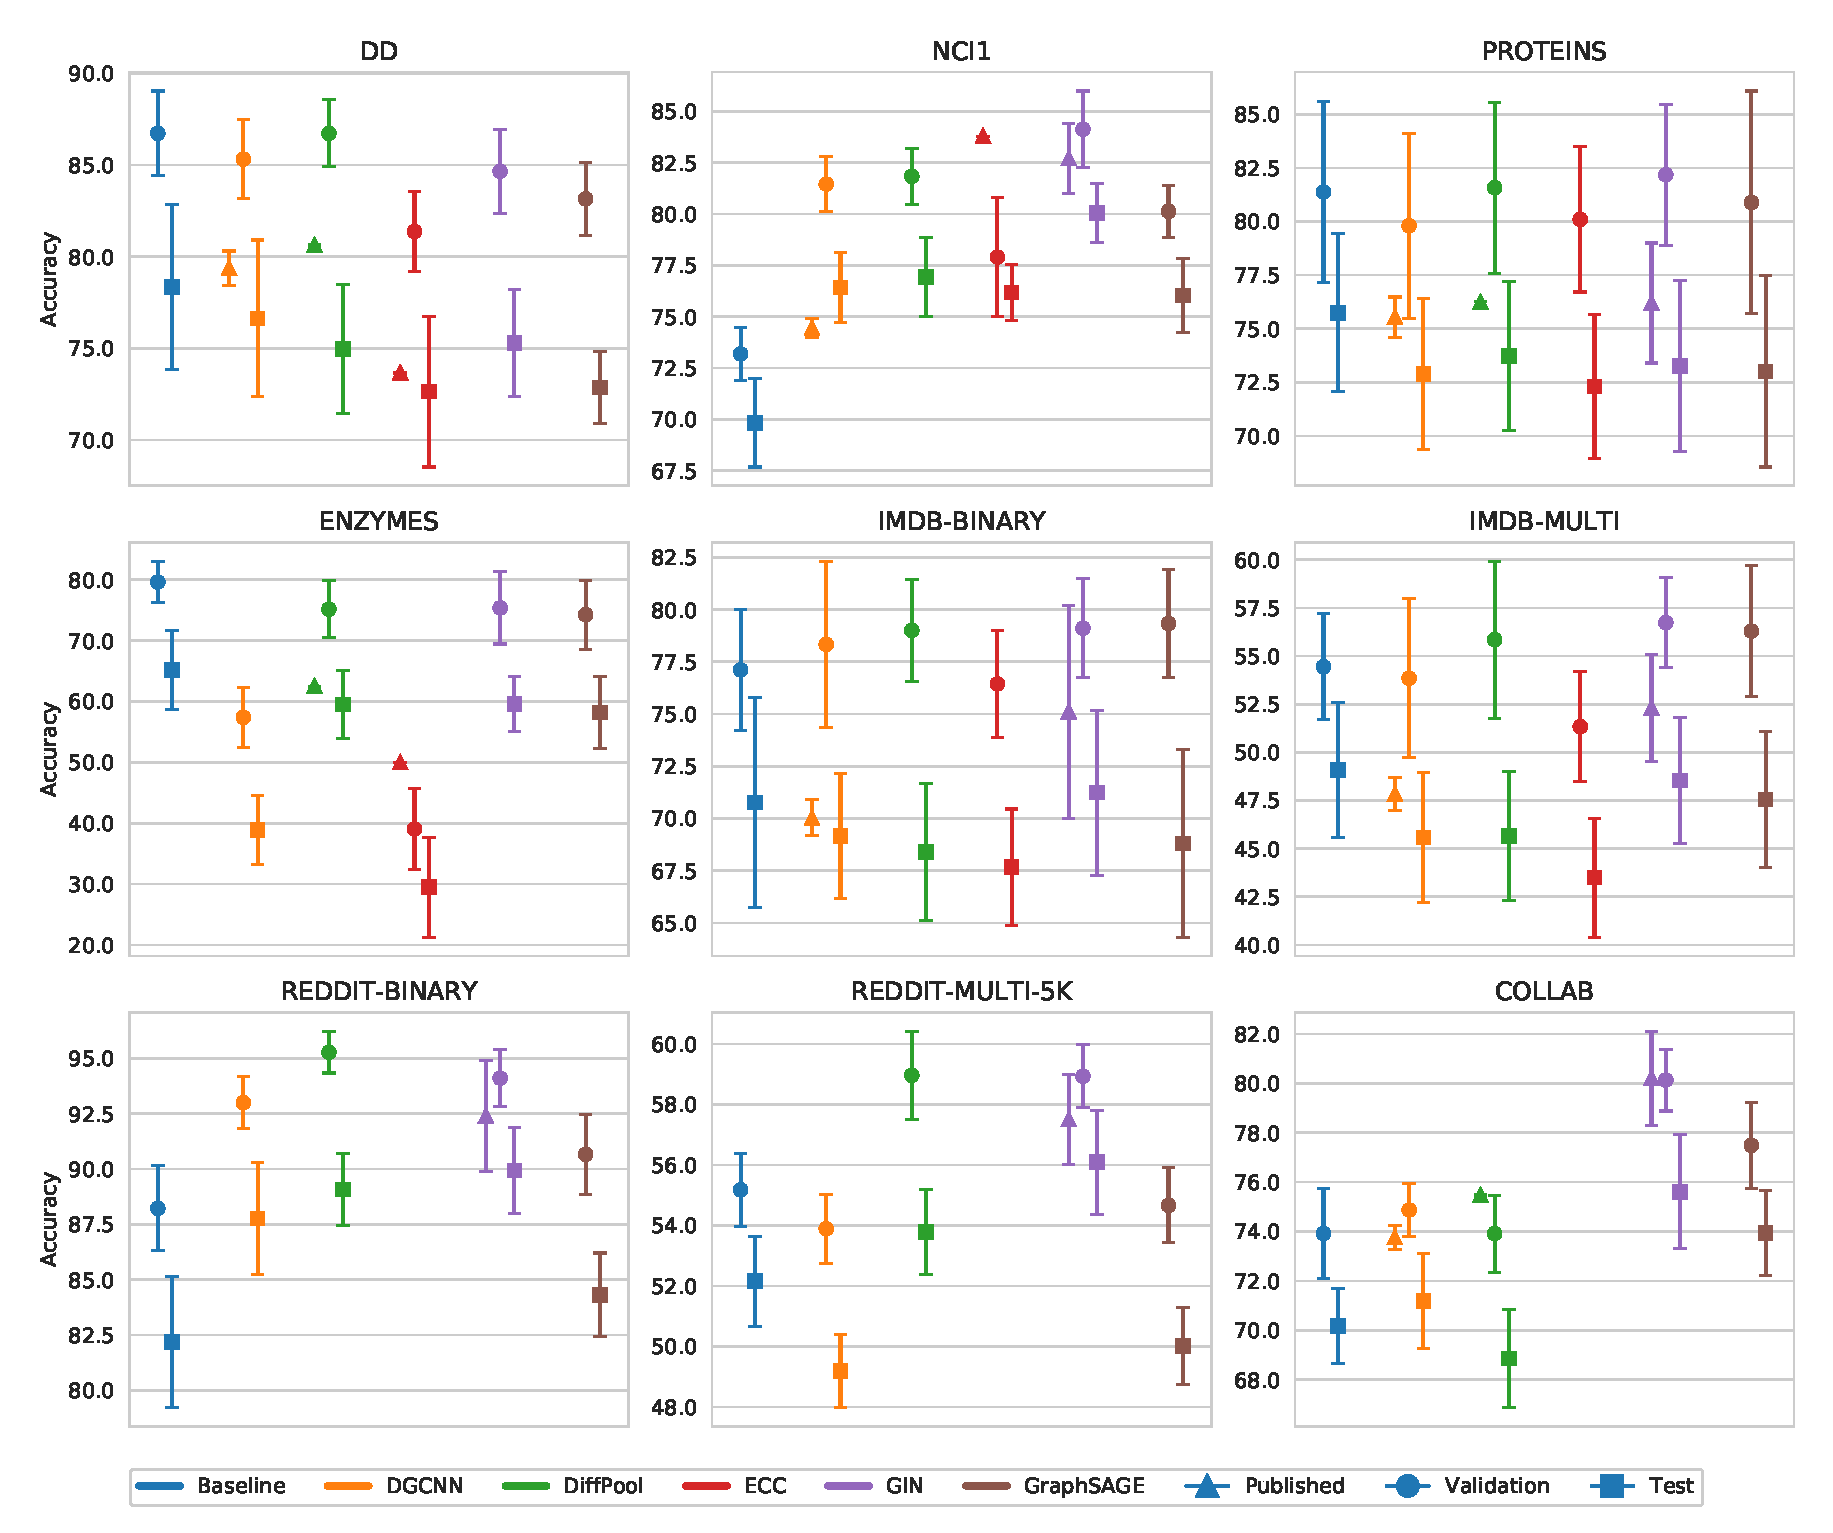
\includegraphics[width=\linewidth]{Figures/Chapter4/07-comparison-results.eps}
    \caption{Results.}
    \label{fig:comparison-plot}
\end{figure}

\subsection{Insights from Hyper-parameter Analysis}
As a follow-up study, we analyze how sensitive the \glspl{dgn} are to changes in the hyper-parameters. In other words, we study how drastically, and if at all, performances vary when varying some relevant hyper-parameters. This would give insights on several practical matters such as which network one can train in the initial phases of an experimental study, in order to get a sensible baseline to build from. To do so, we use validation accuracy as a proxy for test accuracy. First, we collect \emph{post-hoc} all the validation scores obtained by the different models; then, we group the model performances obtained with a fixed choice of a hyper-parameter. We focus on two hyper-parameters that are of relevance for \glspl{dgn}: number of \glspl{gcl}, and dimension of the representation obtained by the network. Figure \ref{fig:nci1-layer} shows a violin plot displaying how the validation performance changes while fixing the number of \glspl{gcl} and optimizing the rest of the hyper-parameters. It can be observed how the performances of GIN are relatively stable with respect to the change in number of layers, while obtaining the highest performances. The figure shows that GIN obtains better performances when the number of \glspl{gcl} is higher than one. The other model performances are fairly stable to the change in number of layers, but we notice an extreme variability in performances (such as with GraphSAGE) which indicates that proper hyper-parameter tuning is essential to get good performances. Figure \ref{fig:nci1-layer} displays the change in performance while fixing the embedding dimension.  From the figure, it appears that GIN performs better with a smaller embedding dimension. This might be partially explained by the theoretical power of GIN, which however makes it prone to overfitting.

\begin{figure}[h!]
    \centering
    \begin{subfigure}[b]{0.49\textwidth}
        \centering
        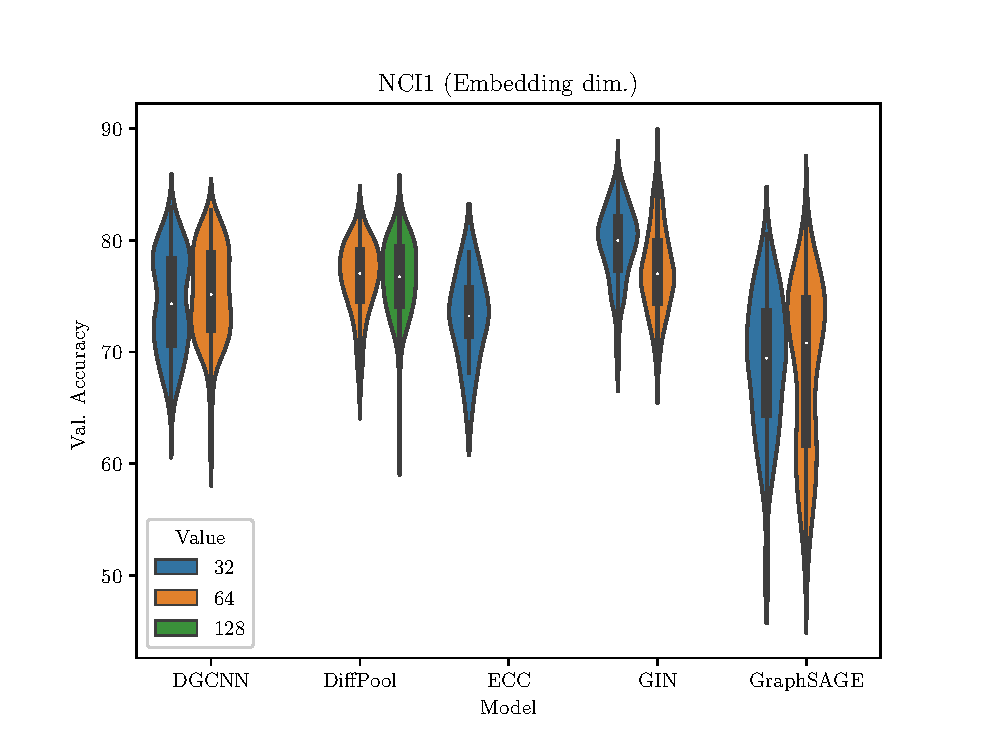
\includegraphics[width=\textwidth]{Figures/Chapter4/nci1-embedding.eps}
        \caption{Embedding dimension.}
        \label{fig:nci1-layer}
    \end{subfigure}
    \hfill
    \begin{subfigure}[b]{0.49\textwidth}
        \centering
        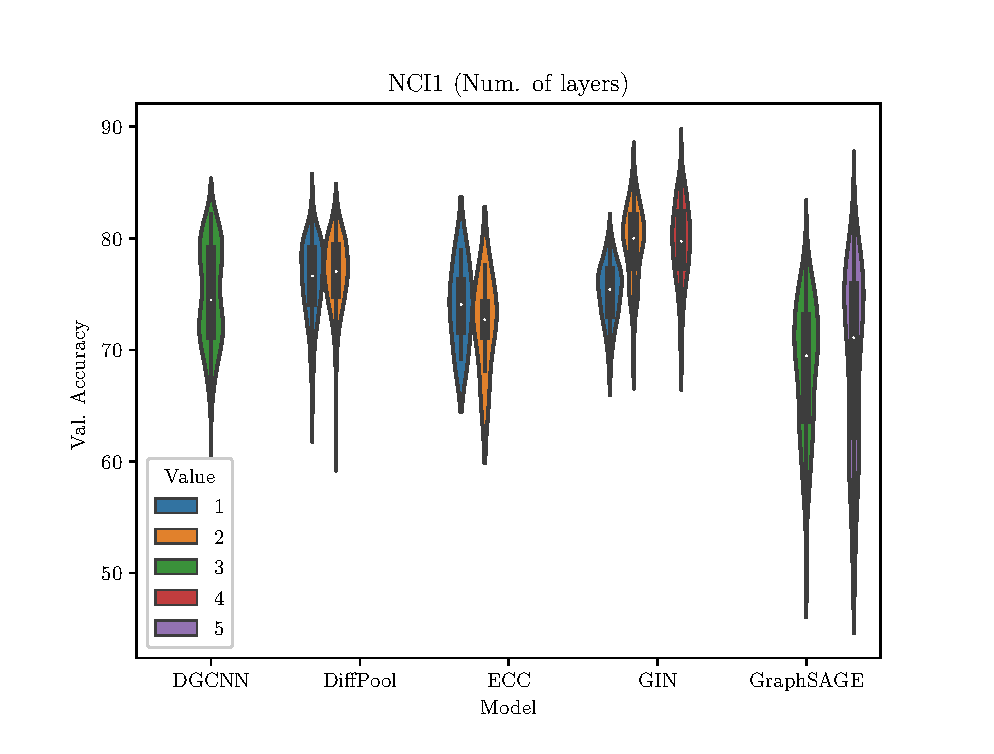
\includegraphics[width=\textwidth]{Figures/Chapter4/nci1-layers.eps}
        \caption{Number of layers.}
        \label{fig:nci1-emb}
    \end{subfigure}
       \caption{The change in validation performances observed on the NCI1 dataset, while optimizing with a fixed number of layers \textsc{(a)} or fixed graph embedding dimension.}
       \label{fig:nci1-posthoc}
\end{figure}

In Figure \ref{fig:collab-layer} and Figure \ref{fig:collab-layer}, we repeat a similar analysis on the COLLAB dataset without using degree information. We notice the same trend with GIN, which requires at least two \glspl{gcl} to obtain good performances. However, there seems not to be a relevant change in performance when using four instead of two \glspl{gcl}. On the contrary, increasing the number of DiffPool layers from one to two has the effect of boosting the accuracy by approximately 10 percentage points on average. However, we also notice from the elongation of the violin that DiffPool is extremely challenging to optimize on this dataset. In Figure \ref{fig:collab-emb}, we show the same analysis but focusing on the embedding dimension. Once again, the trend of Figure \ref{fig:nci1-emb} appears from GIN, where a larger embedding dimension results in a decreased performance. As regards the other models, it seems that there is no effect obtained by varying the embedding dimension, as the violin for the different choices look specular.

\begin{figure}[h!]
    \centering
    \begin{subfigure}[b]{0.49\textwidth}
        \centering
        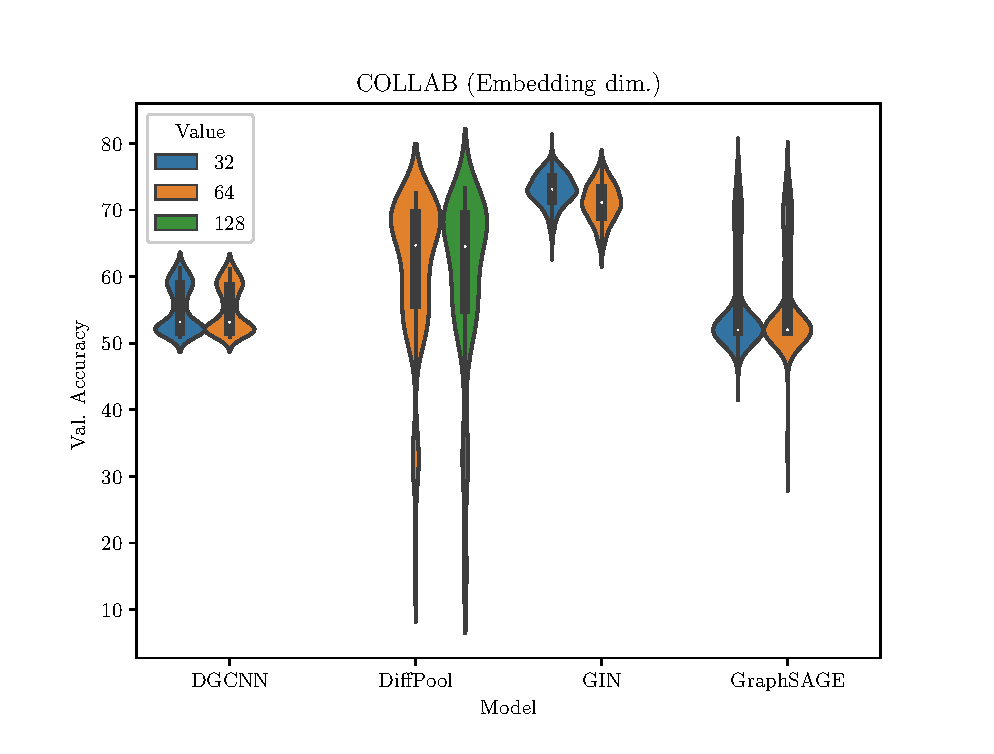
\includegraphics[width=\textwidth]{Figures/Chapter4/collab-embedding.eps}
        \caption{Embedding dimension.}
        \label{fig:collab-layer}
    \end{subfigure}
    \hfill
    \begin{subfigure}[b]{0.49\textwidth}
        \centering
        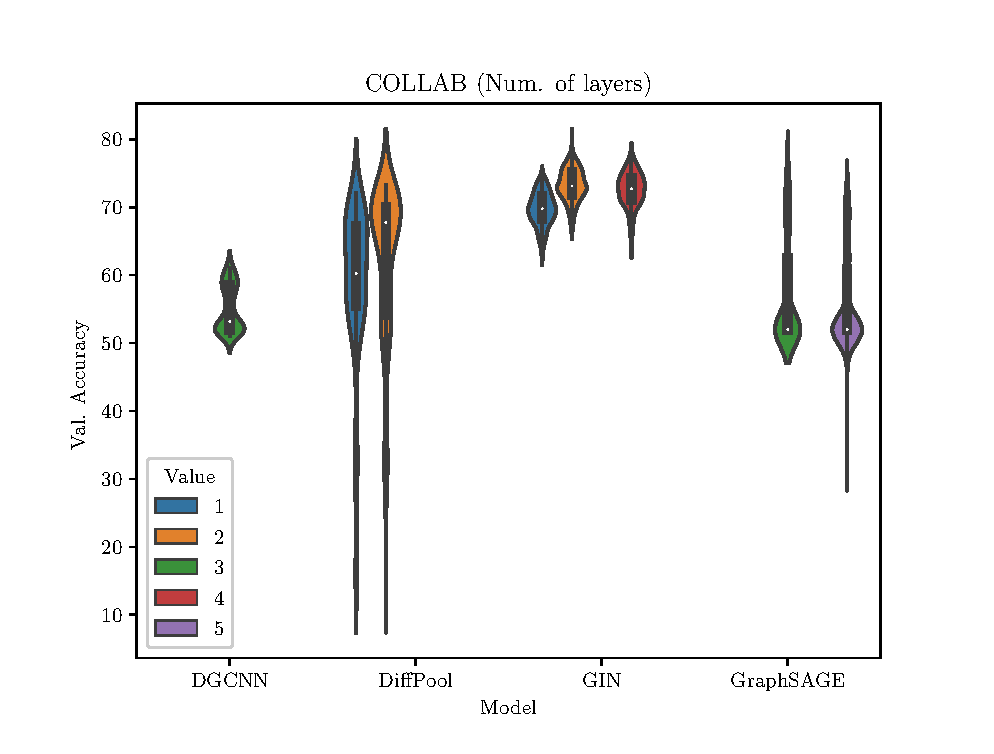
\includegraphics[width=\textwidth]{Figures/Chapter4/collab-layers.eps}
        \caption{Number of layers.}
        \label{fig:collab-emb}
    \end{subfigure}
       \caption{The change in validation performances observed on the COLLAB dataset, while optimizing with a fixed number of layers \textsc{(a)} or fixed graph embedding dimension.}
       \label{fig:collab-posthoc}
\end{figure}

Figure \ref{fig:collab-degree-layer} and Figure \ref{fig:collab-degree-emb} show the same results when the degree features is added to the training graphs. In particular, in Figure \ref{fig:collab-degree-layer} we see that adding the degree might allow GIN to use a higher number of layers to increase performance. For the other models, it appears like changing the number of layers does not provide and substantial change in performance.
Finally, the plot  of Figure \ref{fig:collab-degree-emb} looks very similar to that of Figure \ref{fig:collab-emb}, but the effect of the embedding dimension for GIN is less noticeable.

\begin{figure}[h!]
    \centering
    \begin{subfigure}[b]{0.49\textwidth}
        \centering
        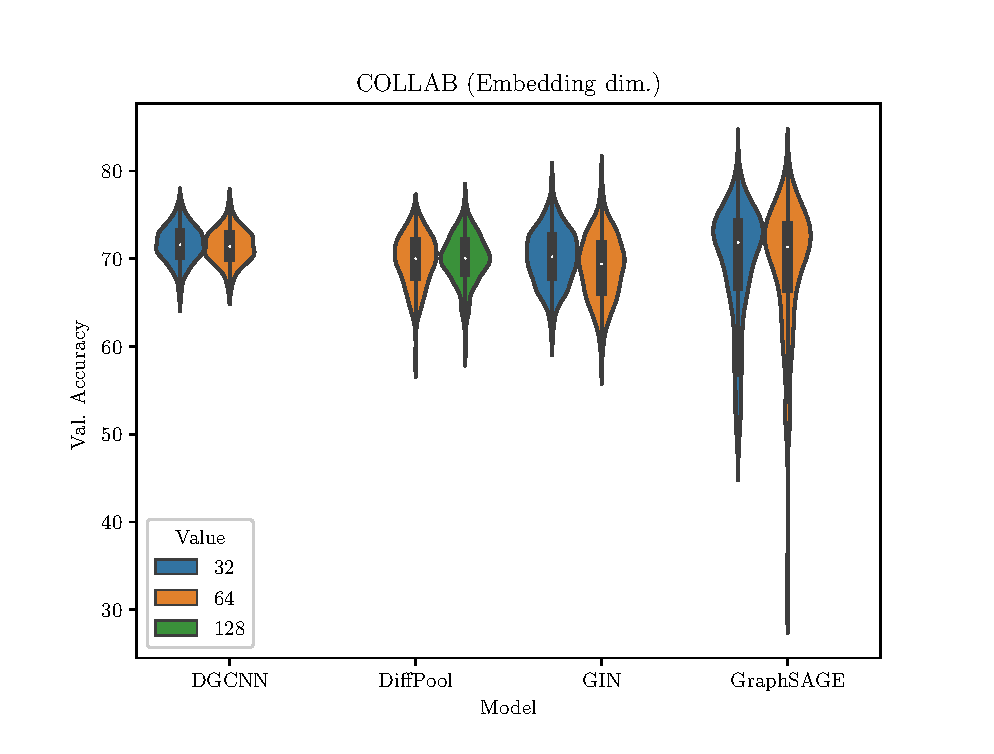
\includegraphics[width=\textwidth]{Figures/Chapter4/collab-degree-embedding.eps}
        \caption{Embedding dimension.}
        \label{fig:collab-degree-layer}
    \end{subfigure}
    \hfill
    \begin{subfigure}[b]{0.49\textwidth}
        \centering
        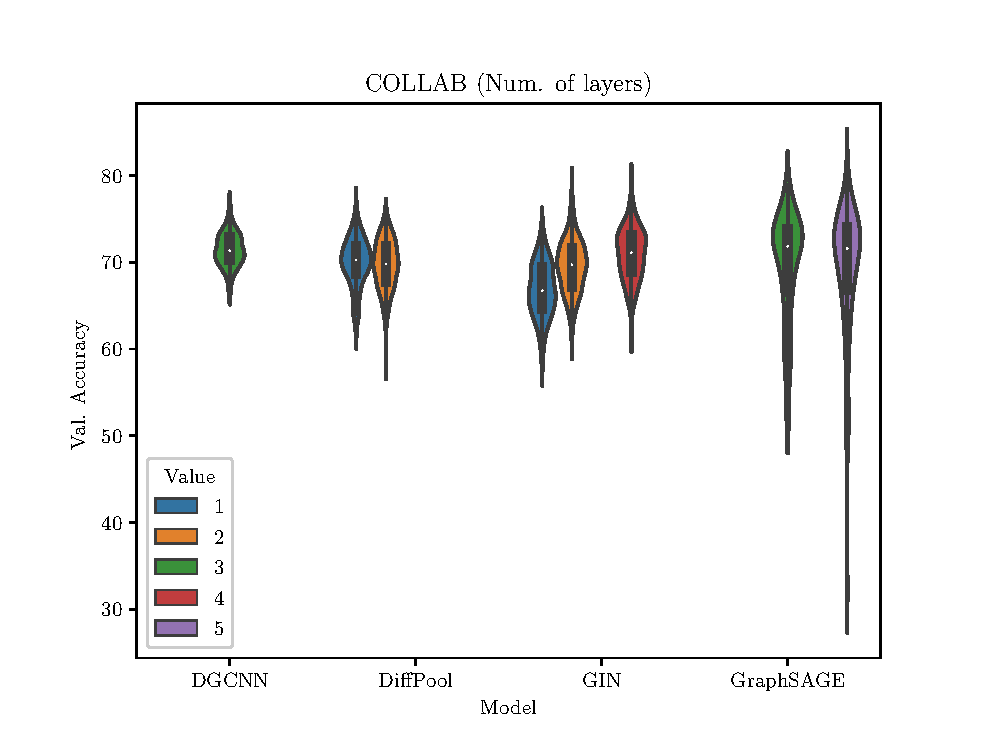
\includegraphics[width=\textwidth]{Figures/Chapter4/collab-degree-layers.eps}
        \caption{Number of layers.}
        \label{fig:collab-degree-emb}
    \end{subfigure}
       \caption{The change in validation performances observed on the COLLAB dataset (using the degree feature), while optimizing with a fixed number of layers \textsc{(a)} or fixed graph embedding dimension.}
       \label{fig:collab-degree-posthoc}
\end{figure}

These results show once again how it is easy to reason about the behavior of \glspl{dgn} once the experimental setup is transparent and the models are evaluated fairly.
\chapter{Case Study: Prediction of Dynamical Properties of Biochemical Pathways using Deep Graph Networks}\label{ch:prediction-biochemical-dgn}

In this chapter, we present an application of Deep Learning techniques on graphs to a life sciences problem related to computational biology. Specifically, we apply Deep Graph Networks to process biochemical pathways, \ie dynamical systems that model the complex interactions between molecules at the biochemical level. Biochemical pathways can be represented as a particular form of bipartite graphs known as Petri networks, which allow to study several properties of such systems. Here, we focus on the property of concentration robustness. To be measured, concentration robustness requires to perform time-expensive simulations. Here, we opt for an approximate but reliable solution, which is orders of magnitude faster to compute. Through processing of the Petri network associated to the biochemical pathway with Deep Graph Networks, we show experimentally that it is possible to build a model that predicts concentration robustness rapidly and with a satisfactory level of accuracy.

\section{Introduction and Motivation}
In order to understand the mechanisms underlying the functioning of living cells, it is necessary to analyze their activities at the biochemical level. Biochemical pathways (or pathways, in short) are complex dynamical systems in which molecules interact with each other through chemical reactions. In these reactions, molecules can take the role of reactant, product, promoter or inhibitor. The dynamics of a pathway are determined by the variation over time of the concentration of its molecules. To study these dynamics, two methodologies are traditionally employed. One consists in modelling the pathway as a system of \glspl{ode}, derived from the application of chemical kinetics laws such as the law of mass action. In cases where pathways involve molecules available in small concentrations, which make the dynamics of reactions sensitive to random events, stochastic modelling and simulation approaches are preferred. These are usually variants of the well-known Gillespie's simulation algorithm \cite{?}. The use of these modelling tools allows to investigate dynamical properties of biochemical pathways such as the reachability of steady states, the occurrence of oscillatory behaviors, causalities between molecular species, and robustness. However, quantitatively measuring these properties often requires to execute a large number of numerical or stochastic simulation, which in turn are time-consuming and computationally intensive.

Given their nature, one widely used formalism to represent biochemical pathways is that of graphs. Many different graphical notations of pathways exist in the literature (see, e.g., \citet{?}), most of which represent molecules as nodes, and reactions as multi-edges or as additional nodes. Using graphs to represent pathways is convenient for three main reasons. Firstly, they provide a quite natural visual representation of the reactions occurring in the pathway. Secondly, they enable the study of the pathway dynamics through methods such as network and structural analysis. Thirdly, graphs can easily be transformed into \glspl{ode} or stochastic models, to apply standard numerical simulation techniques.

In this study, we investigate whether predicting dynamical properties of biochemical pathways from the structure of their associated graphs is possible; and if so, to what extent. In other words, our main assumption is that the dynamics of the biological system modeled by the pathway can be correlated to the structural properties of the graph by which it is represented. If the assumption is correct, the positive implications are two-fold: on one hand, a good predictive model of desired biochemical properties could, in principle, replace numerical or stochastic simulations whenever time and computational budgets are limited. On the other hand, it could allow to predict the properties even in cases where the quantitative information is not available, for example whenever numerical or stochastic simulation methods cannot be applied.

The main idea behind this work is to use of Deep Graph Networks to learn structural features of pathways represented as Petri networks (or Petri nets, in short), which are used to predict a property of interest. Here, we focus on the assessment of the dynamical property of robustness, defined as the the ability of a pathway to preserve its dynamics despite the perturbation of some parameters or initial conditions. More specifically, given a pathway and a pair of molecular species (called \emph{input} and \emph{output} species), the robustness measures how much the concentration of the output species at the steady state is influenced by perturbations of the initial concentration of the input species. This is a notion of \emph{concentration robustness} \citep{?} which is to some extent correlated with the notion of global sensitivity \citep{?}. Robustness makes up for a perfect candidate to test our approach, as its assessment is time-consuming and computationally intensive, requiring a huge number of simulations to explore the parameters space.

The initial part of this work focuses on the creation of a dataset suited to train the \gls{dgn}. We start from collecting 706 curated pathway models in SBML format from the BioModels\footnote{BioModels: \url{https://www.ebi.ac.uk/biomodels/}} database \citep{?}, which were initially converted into Petri nets. For every pathway in this initial dataset, the robustness of every possible pair of input and output species has been computed through \gls{ode}-based simulations. Then, these robustness values have been transformed into binary indicators of whether robustness holds for a given pathway and input/output species. Lastly, for each pathway and for each input/output species in that pathway, the induced subgraphs containing the input and output nodes (as well as other nodes that influence the pathway dynamics) have been extracted. To summarize, the final dataset obtained with this preparatory phase consists of a set of subgraphs, each associated to a pair of input/output molecular species, and their respective robustness indicator. The predictive task is thus one of binary classification: specifically, given a subgraph and two nodes corresponding to the input and output species, the model should correctly classify them as robust or not.

We model the task with a \gls{dgn} to learn structural features from the subgraphs and compute a graph embedding that is passed to a \gls{mlp} classifier. The performances of the model are assessed according to a rigorous framework similar to the one developed in \ref{sec:comparison-exp-setup}. Our experimental results show that we are indeed able to predict robustness with reasonable accuracy. We also conduct a follow-up investigation of how the architectural choices, such as type of graph convolutional layer and number of layer, impact performances. The analysis suggests that the depth of the \gls{dgn}, in terms of number of layers, plays an important role in capturing the right features that correlate the subgraph structure to the robustness, and that deep \glspl{dgn} perform better at this task.

To our knowledge, this is the first work that addresses the problem of predicting dynamical, properties of pathways on a large scale using Deep Learning. In contrast, other approaches in the literature mainly focus on inferring the parameters of a single pathway, or the relationships between its species. We believe this work has great potential in helping understand the functioning of living cells, by serving as a fast, and computationally friendlier, alternative to performing expensive simulations in the assessment of pathway properties.

\section{Background}\label{sect:background}
In this section, we provide the necessary formal background to understand the modeling of biochemical pathways with Petri nets, and the dynamical property of concentration robustness.

\subsection{Pathway Petri Nets}\label{sec:ppn}
Biochemical pathways are essentially sets of chemical reactions of the form:
\[
c_1 S_1 + c_2 S_2 + \ldots
\xrightarrow{k}
c_1' P_1 + c_2' P_2 \ldots,
\]
where $S_i,P_i$ are molecules (\emph{reactants} and \emph{products}, respectively), $c_i, c_i' \in \Natural$ are \emph{stoichiometric coefficients} expressing the multiplicities of reactants and products involved in the reaction, and $k \in \Real_{\geq 0}$ is the \emph{kinetic constant}, used to compute the reaction rate according to standard chemical kinetic laws such as the law of mass action. Besides reactants and products, the reactions of a biochemical pathway often include in their description other molecules, called \emph{modifiers}. These are not consumed nor produced by the reaction, but act either as \emph{promoters} or as \emph{inhibitors}, meaning that they can increase or decrease the reaction rate, respectively. Although these molecules are not listed among reactants and products, they do have a role in the kinetic formula, which no longer follows the mass action principle in this case. For example, in the SBML language \citep{?}, a standard XML-based modeling language for biochemical pathways, reactions can be associated with a number of modifiers, whose concentration is used in the kinetic formula of the reaction. In Figure \ref{subfig:example-reactions} we show a table describing the set of reactions describing a biochemical pathway (first column), some of which include a modifier (second column), namely $A$ for the third reaction, and $F$ for the sixth. Each reaction is associated with its kinetic formula (third column), that, for simplicity, we reference through an alias of the form $\mathsf{r}i$ with $i = 1, \ldots, 7$. Using the kinetic formulas of the two reactions with modifiers as an example, it is clear that $A$ acts as a promoter (meaning that the reaction rate is proportional to the concentration of $A$) and that $F$ acts as inhibitor (meaning that the reaction rate is inversely proportional to the concentration of $F$). Kinetic formulas can then be used to construct a system of \glspl{ode} as shown in Figure \ref{subfig:example-odes}.

\begin{figure}
\begin{subfigure}[b]{0.49\linewidth}
    \[\def\arraystretch{1.2}
    \begin{array}{ccl}
      \mbox{Reaction } & \mbox{ Modifiers } & \mbox{ Kinetics}\\
      \hline
      \SF{A} + \SF{B} \rightarrow 2\SF{B} &      & \SF{r}1 = k_1\SF{AB}\\
      \SF{B} \rightarrow \SF{A}      &      & \SF{r}2 = k_2\SF{B}\\
      \SF{C} + \SF{D} \rightarrow \SF{E}  & \SF{A}    & \SF{r}3 = k_3\SF{CDA}\\
      \SF{E} \rightarrow \SF{F}      &      & \SF{r}4 = k_4\SF{E}\\
      \SF{F} \rightarrow \SF{E}      &      & \SF{r}5 = k_5\SF{F}\\
      \SF{G} \rightarrow \SF{H}      & \SF{F}    & \SF{r}6 = \frac{k_6\SF{G}}{1+2 \SF{F}}\\
      \SF{H} \rightarrow \SF{G}      &      & \SF{r}7 = k_7\SF{H}\\
    \end{array}
    \]
\caption{Reactions}\label{subfig:example-reactions}
\end{subfigure}
%
\begin{subfigure}[b]{0.49\linewidth}
\[\def\arraystretch{1.2}
\begin{array}{l}
    \frac{d\SF{A}}{dt} = -k_1\SF{A}B + k_2\SF{B}\\
    \frac{d\SF{B}}{dt} = k_1\SF{AB} - k_2\SF{B}\\
    \frac{d\SF{C}}{dt} = -k_3\SF{CDA}\\
    \frac{d\SF{D}}{dt} = -k_3\SF{CDA}\\
    \frac{d\SF{E}}{dt} = k_3\SF{CDA} - k_4\SF{E} + k_5\SF{F}\\
    \frac{d\SF{F}}{dt} = k_4\SF{E} - k_5\SF{F}\\
    \frac{d\SF{G}}{dt} = -\frac{k_6\SF{G}}{1+2 \SF{F}} + k_7\SF{H}\\
    \frac{d\SF{H}}{dt} = \frac{k_6\SF{G}}{1+2 \SF{F}} - k_7\SF{H}
\end{array}
\]
\caption{ODEs}\label{subfig:example-odes}
\end{subfigure}
%
\caption{An example of biochemical pathway. ({\scriptsize A}) list of reactions with information on modifiers and kinetic formulas. ({\scriptsize B}) the corresponding system of ODEs.}\label{fig:example-pathway}
\end{figure}

A common way to represent biochemical pathways is through Petri nets \cite{?}. The formalism of Petri nets have been originally proposed for the description and analysis of concurrent systems \cite{?}, but has been later adopted to model other kinds of systems, such as biological ones. Several variants of Petri nets have been proposed in the literature. In this work, we consider a version of \emph{continuous} Petri nets \cite{?} with promotion and inhibition edges and general kinetic functions. We call this biologically inspired variant \gls{ppn}. A \gls{ppn} is essentially a bipartite graph with two types of nodes and three types of labelled edges. According to standard Petri nets terminology, the two types of nodes are called \emph{places} and \emph{transitions}. The semantics of a \gls{ppn} in a continuous setting are described by a system of ODEs, with one equation for each place. In the case of pathways, such system corresponds exactly to the one obtained from the chemical reactions shown in Figure \ref{subfig:example-odes}. The state of a \gls{ppn} (called \emph{marking}) is then defined as an assignment of positive real values to the variables of the ODEs. We denote with $\Cal{M}$ the set of all possible markings.

More formally, a \gls{ppn} can be defined as a tuple $\wp = \Tuple{\Cal{P},\Cal{T},\Cal{A}_{S}, \Cal{A}_{P},\Cal{A}_{I},\vartheta,\varsigma,M_0}$ where:
\begin{itemize}
    \item $\Cal{P}$ and $\Cal{T}$ are finite, non empty disjoint sets of places and transitions, respectively;
    \item $\Cal{A}_{S} = ((\Cal{P}\times \Cal{T}) \cup (\Cal{T}\times \Cal{P})$ is a set of standard directed edges;
    \item $\Cal{A}_{P} \subseteq (\Cal{P} \times \Cal{T})$ is the set of promotion edges;
    \item $\Cal{A}_{I} \subseteq (\Cal{P} \times \Cal{T})$ is the set of inhibition edges;
    \item $\varsigma: \Cal{A}_{S} \shortrightarrow \mathbb{N}^{\geq 0}$ weights every standard edge by non-negative integer values;
    \item $\varsigma:\Cal{T} \shortrightarrow (\Cal{M} \rightarrow \mathbb{R}^{\geq 0})$,  is a function that assigns, to each transition, a function that computes a kinetic formula to every possible marking $M \in \Cal{M}$;
    \item $M_0 \in \Cal{M}$ is the initial marking.
\end{itemize}
A visual representation of the \gls{ppn} corresponding to the pathway in Figure \ref{subfig:example-reactions} is shown in Figure \ref{subfig:pathway-petri-net}. The sets of places $\Cal{P}$ and transitions $\Cal{T}$ of a pathway Petri net represent molecular species and reactants, and are displayed as circles and rectangles, respectively. In the figure, places are labeled with the name of the corresponding molecule. The directed edges, depicted as standard arrows, connect reactants to reactions and reactions to products. The weights of the edges (omitted if equal to one) correspond to the stoichiometric coefficients of reactant/product pairs. The sets of promotion and inhibition edges, $\Cal{A}_{P}$ and $\Cal{A}_{I}$, connect molecules to the reactions they promote or inhibit, respectively, and they are displayed as dotted or T-shaped arrows, respectively. The kinetic formulas of reactions (or rather, their aliases defined as in Figure \ref{subfig:pathway-petri-net}), are shown inside the rectangles of the corresponding transitions. As explained previously, molecules connected through promotion edges give a positive contribution to the value of the kinetic formula, while molecules connected through inhibition edges give a negative (inversely proportional) contribution. Finally, the initial marking $M_0$ is not shown in the figure, and it has to be described separately.
\begin{figure*}[h!]
    \centering
    \resizebox{.6\textwidth}{!}{

\tikzset{every picture/.style={line width=0.75pt}} %set default line width to 0.75pt        

\begin{tikzpicture}[x=0.75pt,y=0.75pt,yscale=-1,xscale=1]
%uncomment if require: \path (0,300); %set diagram left start at 0, and has height of 300

%Straight Lines [id:da3576438741903769] 
\draw    (388,210) -- (414.13,177.34) ;
\draw [shift={(416,175)}, rotate = 488.66] [fill={rgb, 255:red, 0; green, 0; blue, 0 }  ][line width=0.08]  [draw opacity=0] (8.93,-4.29) -- (0,0) -- (8.93,4.29) -- cycle    ;
%Straight Lines [id:da5206527388854192] 
\draw    (350,164) -- (376.13,196.66) ;
\draw [shift={(378,199)}, rotate = 231.34] [fill={rgb, 255:red, 0; green, 0; blue, 0 }  ][line width=0.08]  [draw opacity=0] (8.93,-4.29) -- (0,0) -- (8.93,4.29) -- cycle    ;
%Straight Lines [id:da9664135693242828] 
\draw    (388,110) -- (361.87,142.66) ;
\draw [shift={(360,145)}, rotate = 308.65999999999997] [fill={rgb, 255:red, 0; green, 0; blue, 0 }  ][line width=0.08]  [draw opacity=0] (8.93,-4.29) -- (0,0) -- (8.93,4.29) -- cycle    ;
%Straight Lines [id:da3150124855239005] 
\draw    (426,156) -- (399.87,123.34) ;
\draw [shift={(398,121)}, rotate = 411.34000000000003] [fill={rgb, 255:red, 0; green, 0; blue, 0 }  ][line width=0.08]  [draw opacity=0] (8.93,-4.29) -- (0,0) -- (8.93,4.29) -- cycle    ;
%Straight Lines [id:da2531638133399581] 
\draw    (295,160) -- (335,160) ;
%Straight Lines [id:da7978054588524539] 
\draw    (110,160) -- (157,160) ;
\draw [shift={(160,160)}, rotate = 180] [fill={rgb, 255:red, 0; green, 0; blue, 0 }  ][line width=0.08]  [draw opacity=0] (8.93,-4.29) -- (0,0) -- (8.93,4.29) -- cycle    ;
%Straight Lines [id:da5621074466789615] 
\draw    (235,125) -- (279.4,150.51) ;
\draw [shift={(282,152)}, rotate = 209.88] [fill={rgb, 255:red, 0; green, 0; blue, 0 }  ][line width=0.08]  [draw opacity=0] (8.93,-4.29) -- (0,0) -- (8.93,4.29) -- cycle    ;
%Straight Lines [id:da9432384230142636] 
\draw    (235,195) -- (190.6,169.49) ;
\draw [shift={(188,168)}, rotate = 389.88] [fill={rgb, 255:red, 0; green, 0; blue, 0 }  ][line width=0.08]  [draw opacity=0] (8.93,-4.29) -- (0,0) -- (8.93,4.29) -- cycle    ;
%Straight Lines [id:da2732887752012232] 
\draw    (295,160) -- (252.62,183.54) ;
\draw [shift={(250,185)}, rotate = 330.95] [fill={rgb, 255:red, 0; green, 0; blue, 0 }  ][line width=0.08]  [draw opacity=0] (8.93,-4.29) -- (0,0) -- (8.93,4.29) -- cycle    ;
%Straight Lines [id:da8361705783456022] 
\draw    (175,160) -- (217.38,136.46) ;
\draw [shift={(220,135)}, rotate = 510.95] [fill={rgb, 255:red, 0; green, 0; blue, 0 }  ][line width=0.08]  [draw opacity=0] (8.93,-4.29) -- (0,0) -- (8.93,4.29) -- cycle    ;
%Straight Lines [id:da26704871020062715] 
\draw    (110,90) -- (157.05,81.23) ;
\draw [shift={(160,80.68)}, rotate = 529.44] [fill={rgb, 255:red, 0; green, 0; blue, 0 }  ][line width=0.08]  [draw opacity=0] (8.93,-4.29) -- (0,0) -- (8.93,4.29) -- cycle    ;
%Straight Lines [id:da4846937260313433] 
\draw    (40,80.68) -- (87.05,89.45) ;
\draw [shift={(90,90)}, rotate = 190.56] [fill={rgb, 255:red, 0; green, 0; blue, 0 }  ][line width=0.08]  [draw opacity=0] (8.93,-4.29) -- (0,0) -- (8.93,4.29) -- cycle    ;
%Straight Lines [id:da271105016276878] 
\draw    (105,25) -- (157.47,58.39) ;
\draw [shift={(160,60)}, rotate = 212.47] [fill={rgb, 255:red, 0; green, 0; blue, 0 }  ][line width=0.08]  [draw opacity=0] (8.93,-4.29) -- (0,0) -- (8.93,4.29) -- cycle    ;
%Shape: Rectangle [id:dp9228181661849988] 
\draw  [fill={rgb, 255:red, 255; green, 255; blue, 255 }  ,fill opacity=1 ] (20,50) -- (50,50) -- (50,90) -- (20,90) -- cycle ;
%Straight Lines [id:da06467494297119436] 
\draw    (105,25) -- (52.53,58.39) ;
\draw [shift={(50,60)}, rotate = 327.53] [fill={rgb, 255:red, 0; green, 0; blue, 0 }  ][line width=0.08]  [draw opacity=0] (8.93,-4.29) -- (0,0) -- (8.93,4.29) -- cycle    ;
%Shape: Circle [id:dp49236484975772] 
\draw  [fill={rgb, 255:red, 255; green, 255; blue, 255 }  ,fill opacity=1 ] (90,25) .. controls (90,16.72) and (96.72,10) .. (105,10) .. controls (113.28,10) and (120,16.72) .. (120,25) .. controls (120,33.28) and (113.28,40) .. (105,40) .. controls (96.72,40) and (90,33.28) .. (90,25) -- cycle ;
%Shape: Rectangle [id:dp3146550401206405] 
\draw  [fill={rgb, 255:red, 255; green, 255; blue, 255 }  ,fill opacity=1 ] (160,50) -- (190,50) -- (190,90) -- (160,90) -- cycle ;
%Curve Lines [id:da9984566963389516] 
\draw    (190,70) .. controls (250.06,70.4) and (250.75,-32.96) .. (121.95,19.2) ;
\draw [shift={(120,20)}, rotate = 337.56] [fill={rgb, 255:red, 0; green, 0; blue, 0 }  ][line width=0.08]  [draw opacity=0] (8.93,-4.29) -- (0,0) -- (8.93,4.29) -- cycle    ;
%Shape: Circle [id:dp09345090103745823] 
\draw  [fill={rgb, 255:red, 255; green, 255; blue, 255 }  ,fill opacity=1 ] (90,95) .. controls (90,86.72) and (96.72,80) .. (105,80) .. controls (113.28,80) and (120,86.72) .. (120,95) .. controls (120,103.28) and (113.28,110) .. (105,110) .. controls (96.72,110) and (90,103.28) .. (90,95) -- cycle ;
%Straight Lines [id:da5223576478149881] 
\draw    (105,110) -- (105,131) ;
\draw [shift={(105,131)}, rotate = 90] [color={rgb, 255:red, 0; green, 0; blue, 0 }  ][fill={rgb, 255:red, 0; green, 0; blue, 0 }  ][line width=0.75]      (0, 0) circle [x radius= 3.35, y radius= 3.35]   ;
%Shape: Rectangle [id:dp25364205729175127] 
\draw  [fill={rgb, 255:red, 255; green, 255; blue, 255 }  ,fill opacity=1 ] (90,140) -- (120,140) -- (120,180) -- (90,180) -- cycle ;
%Straight Lines [id:da8084682726089965] 
\draw    (40,140.68) -- (87.05,149.45) ;
\draw [shift={(90,150)}, rotate = 190.56] [fill={rgb, 255:red, 0; green, 0; blue, 0 }  ][line width=0.08]  [draw opacity=0] (8.93,-4.29) -- (0,0) -- (8.93,4.29) -- cycle    ;
%Straight Lines [id:da8278541197200837] 
\draw    (40,180) -- (87.05,171.23) ;
\draw [shift={(90,170.68)}, rotate = 529.44] [fill={rgb, 255:red, 0; green, 0; blue, 0 }  ][line width=0.08]  [draw opacity=0] (8.93,-4.29) -- (0,0) -- (8.93,4.29) -- cycle    ;
%Shape: Circle [id:dp5697702501712039] 
\draw  [fill={rgb, 255:red, 255; green, 255; blue, 255 }  ,fill opacity=1 ] (20,137) .. controls (20,128.72) and (26.72,122) .. (35,122) .. controls (43.28,122) and (50,128.72) .. (50,137) .. controls (50,145.28) and (43.28,152) .. (35,152) .. controls (26.72,152) and (20,145.28) .. (20,137) -- cycle ;
%Shape: Circle [id:dp027027959729662543] 
\draw  [fill={rgb, 255:red, 255; green, 255; blue, 255 }  ,fill opacity=1 ] (20,183) .. controls (20,174.72) and (26.72,168) .. (35,168) .. controls (43.28,168) and (50,174.72) .. (50,183) .. controls (50,191.28) and (43.28,198) .. (35,198) .. controls (26.72,198) and (20,191.28) .. (20,183) -- cycle ;
%Shape: Circle [id:dp7929646959402241] 
\draw  [fill={rgb, 255:red, 255; green, 255; blue, 255 }  ,fill opacity=1 ] (160,160) .. controls (160,151.72) and (166.72,145) .. (175,145) .. controls (183.28,145) and (190,151.72) .. (190,160) .. controls (190,168.28) and (183.28,175) .. (175,175) .. controls (166.72,175) and (160,168.28) .. (160,160) -- cycle ;
%Shape: Rectangle [id:dp05655391624383377] 
\draw  [fill={rgb, 255:red, 255; green, 255; blue, 255 }  ,fill opacity=1 ] (220,115) -- (250,115) -- (250,155) -- (220,155) -- cycle ;
%Shape: Rectangle [id:dp05796590340987029] 
\draw  [fill={rgb, 255:red, 255; green, 255; blue, 255 }  ,fill opacity=1 ] (220,165) -- (250,165) -- (250,205) -- (220,205) -- cycle ;
%Shape: Circle [id:dp13273124949760895] 
\draw  [fill={rgb, 255:red, 255; green, 255; blue, 255 }  ,fill opacity=1 ] (280,160) .. controls (280,151.72) and (286.72,145) .. (295,145) .. controls (303.28,145) and (310,151.72) .. (310,160) .. controls (310,168.28) and (303.28,175) .. (295,175) .. controls (286.72,175) and (280,168.28) .. (280,160) -- cycle ;
%Straight Lines [id:da9347007050049654] 
\draw    (335.29,154.43) -- (335.26,165.81) ;
%Straight Lines [id:da20553639689795267] 
\draw    (336,154.43) -- (335.97,165.81) ;
%Shape: Rectangle [id:dp30165349356224813] 
\draw  [fill={rgb, 255:red, 255; green, 255; blue, 255 }  ,fill opacity=1 ] (380,145) -- (380,175) -- (340,175) -- (340,145) -- cycle ;
%Shape: Rectangle [id:dp05448702121100979] 
\draw  [fill={rgb, 255:red, 255; green, 255; blue, 255 }  ,fill opacity=1 ] (436,145) -- (436,175) -- (396,175) -- (396,145) -- cycle ;
%Shape: Circle [id:dp37659499504730287] 
\draw  [fill={rgb, 255:red, 255; green, 255; blue, 255 }  ,fill opacity=1 ] (373,110) .. controls (373,101.72) and (379.72,95) .. (388,95) .. controls (396.28,95) and (403,101.72) .. (403,110) .. controls (403,118.28) and (396.28,125) .. (388,125) .. controls (379.72,125) and (373,118.28) .. (373,110) -- cycle ;
%Shape: Circle [id:dp13055596917815526] 
\draw  [fill={rgb, 255:red, 255; green, 255; blue, 255 }  ,fill opacity=1 ] (373,210) .. controls (373,201.72) and (379.72,195) .. (388,195) .. controls (396.28,195) and (403,201.72) .. (403,210) .. controls (403,218.28) and (396.28,225) .. (388,225) .. controls (379.72,225) and (373,218.28) .. (373,210) -- cycle ;

% Text Node
\draw (26,62) node [anchor=north west][inner sep=0.75pt]   [align=left] {$\mathsf{r2}$};
% Text Node
\draw (168,62) node [anchor=north west][inner sep=0.75pt]   [align=left] {$\mathsf{r1}$};
% Text Node
\draw (97,153) node [anchor=north west][inner sep=0.75pt]   [align=left] {$\mathsf{r3}$};
% Text Node
\draw (227,127) node [anchor=north west][inner sep=0.75pt]   [align=left] {$\mathsf{r4}$};
% Text Node
\draw (227,178) node [anchor=north west][inner sep=0.75pt]   [align=left] {$\mathsf{r5}$};
% Text Node
\draw (352,154) node [anchor=north west][inner sep=0.75pt]   [align=left] {$\mathsf{r6}$};
% Text Node
\draw (409,154) node [anchor=north west][inner sep=0.75pt]   [align=left] {$\mathsf{r7}$};

% Text Node
\draw (98,18) node [anchor=north west][inner sep=0.75pt]   [align=left] {$\mathsf{B}$};
% Text Node
\draw (98,89) node [anchor=north west][inner sep=0.75pt]   [align=left] {$\mathsf{A}$};
% Text Node
\draw (28,130) node [anchor=north west][inner sep=0.75pt]   [align=left] {$\mathsf{C}$};
% Text Node
\draw (28,177) node [anchor=north west][inner sep=0.75pt]   [align=left] {$\mathsf{D}$};
% Text Node
\draw (168,153) node [anchor=north west][inner sep=0.75pt]   [align=left] {$\mathsf{E}$};
% Text Node
\draw (289,153) node [anchor=north west][inner sep=0.75pt]   [align=left] {$\mathsf{F}$};
% Text Node
\draw (381,103) node [anchor=north west][inner sep=0.75pt]   [align=left] {$\mathsf{G}$};
% Text Node
\draw (381,203) node [anchor=north west][inner sep=0.75pt]   [align=left] {$\mathsf{H}$};
% Text Node
\draw (232,24) node [anchor=north west][inner sep=0.75pt]   [align=left] {$\mathsf{2}$};


\end{tikzpicture}}
    \caption{The Pathway Petri Net corresponding to the reactions described in Figure \ref{subfig:example-reactions}}
    \label{subfig:pathway-petri-net}
\end{figure*}

In this work, we use a variant of \glspl{ppn} where all the information unrelated to the structure of the pathway is discarded. Specifically, we ignore information about:
\begin{itemize}
    \item kinetic formulas;
    \item multiplicities of reactants and products (\ie edge labels);
    \item the initial marking $M_0$.
\end{itemize}
Basically, for our purposes, a \gls{ppn} is a tuple $\wp = \Tuple{\Cal{P},\Cal{T},\Cal{A}_{S}, \Cal{A}_{P},\Cal{A}_{I}}$ where the irrelevant components have been omitted. We rewrite this object, according to the graph notation introduced in Section \ref{sec:graphs}, into a \keyword{pathway graph} $G = \Tuple{\Cal{V}_G, \Cal{E}_G}$. To do so, we first define the following nodes and edges subsets:
\begin{itemize}
    \item $\Cal{V}_{G}^{\Fun{mol}} = \Cal{P}$ is the set of molecules;
    \item $\Cal{V}_{G}^{\Fun{rx}} = \Cal{T}$ is the set of reactions;
    \item $\Cal{E}_{G}^{\Fun{std}} = \Cal{A}_S$ is the set of standard edges;
    \item $\Cal{E}_{G}^{\Fun{pro}} = \Cal{A}_P$ is the set of promoter edges;
    \item $\Cal{E}_{G}^{\Fun{inh}} = \Cal{A}_I$ is the set of inhibitor edges,
\end{itemize}
where $\Cal{V}_{G}^{\Fun{mol}} \Inter \Cal{V}_{G}^{\Fun{rx}} = \emptyset$ and $\Cal{E}_{G}^{\Fun{std}} \Inter \Cal{E}_{G}^{\Fun{pro}} \Inter \Cal{E}_{G}^{\Fun{inh}} = \emptyset$. Then, we simply set $\Cal{V}_G = \Cal{V}_G^{\Fun{mol}} \Union \Cal{V}_G^{\Fun{rx}}$ and $\Cal{E}_G = \Cal{E}_G^{\Fun{std}} \Union \Cal{E}_G^{\Fun{pro}} \Union \Cal{E}_G^{\Fun{inh}}$.
Using the biochemical pathway of Figure \ref{fig:example-pathway} as reference, its associated pathway graph is shown in Figure \ref{fig:pathway-graph}.
\begin{figure*}[h!]
    \centering
    \resizebox{.6\textwidth}{!}{

\tikzset{every picture/.style={line width=0.75pt}} %set default line width to 0.75pt

\begin{tikzpicture}[x=0.75pt,y=0.75pt,yscale=-1,xscale=1]
%uncomment if require: \path (0,300); %set diagram left start at 0, and has height of 300

%Straight Lines [id:da289255485986883]
\draw    (100,56) -- (135.62,83.18) ;
\draw [shift={(138,85)}, rotate = 217.35] [fill={rgb, 255:red, 0; green, 0; blue, 0 }  ][line width=0.08]  [draw opacity=0] (5.36,-2.57) -- (0,0) -- (5.36,2.57) -- cycle    ;

% Text Node
\draw  [fill={rgb, 255:red, 255; green, 255; blue, 255 }  ,fill opacity=1 ]  (38,78) -- (62,78) -- (62,112) -- (38,112) -- cycle  ;
\draw (50,95) node   [align=left] {\begin{minipage}[lt]{13.600000000000001pt}\setlength\topsep{0pt}
\begin{center}
\end{center}

\end{minipage}};
% Text Node
\draw  [fill={rgb, 255:red, 255; green, 255; blue, 255 }  ,fill opacity=1 ]  (100, 55.5) circle [x radius= 13.2, y radius= 13.2]   ;
\draw (100,55.5) node   [align=left] {\begin{minipage}[lt]{14.96pt}\setlength\topsep{0pt}
\begin{center}
\SF{B}
\end{center}

\end{minipage}};
% Text Node
\draw  [fill={rgb, 255:red, 255; green, 255; blue, 255 }  ,fill opacity=1 ]  (138,78) -- (162,78) -- (162,112) -- (138,112) -- cycle  ;
\draw (150,95) node   [align=left] {\begin{minipage}[lt]{13.600000000000001pt}\setlength\topsep{0pt}
\begin{center}
\end{center}

\end{minipage}};
% Text Node
\draw  [fill={rgb, 255:red, 255; green, 255; blue, 255 }  ,fill opacity=1 ]  (100, 135.5) circle [x radius= 13.2, y radius= 13.2]   ;
\draw (100,135.5) node   [align=left] {\begin{minipage}[lt]{14.96pt}\setlength\topsep{0pt}
\begin{center}
\SF{A}
\end{center}

\end{minipage}};
% Text Node
\draw  [fill={rgb, 255:red, 255; green, 255; blue, 255 }  ,fill opacity=1 ]  (39, 175.5) circle [x radius= 13.2, y radius= 13.2]   ;
\draw (39,175.5) node   [align=left] {\begin{minipage}[lt]{14.96pt}\setlength\topsep{0pt}
\begin{center}
\SF{C}
\end{center}

\end{minipage}};
% Text Node
\draw  [fill={rgb, 255:red, 255; green, 255; blue, 255 }  ,fill opacity=1 ]  (39, 215.5) circle [x radius= 13.2, y radius= 13.2]   ;
\draw (39,215.5) node   [align=left] {\begin{minipage}[lt]{14.96pt}\setlength\topsep{0pt}
\begin{center}
\SF{D}
\end{center}

\end{minipage}};
% Text Node
\draw  [fill={rgb, 255:red, 255; green, 255; blue, 255 }  ,fill opacity=1 ]  (88,178) -- (112,178) -- (112,212) -- (88,212) -- cycle  ;
\draw (100,195) node   [align=left] {\begin{minipage}[lt]{13.600000000000001pt}\setlength\topsep{0pt}
\begin{center}
\end{center}

\end{minipage}};
% Text Node
\draw  [fill={rgb, 255:red, 255; green, 255; blue, 255 }  ,fill opacity=1 ]  (159, 195.5) circle [x radius= 13.2, y radius= 13.2]   ;
\draw (159,195.5) node   [align=left] {\begin{minipage}[lt]{14.96pt}\setlength\topsep{0pt}
\begin{center}
\SF{E}
\end{center}

\end{minipage}};
% Text Node
\draw  [fill={rgb, 255:red, 255; green, 255; blue, 255 }  ,fill opacity=1 ]  (198,148) -- (222,148) -- (222,182) -- (198,182) -- cycle  ;
\draw (210,165) node   [align=left] {\begin{minipage}[lt]{13.600000000000001pt}\setlength\topsep{0pt}
\begin{center}
\end{center}

\end{minipage}};
% Text Node
\draw  [fill={rgb, 255:red, 255; green, 255; blue, 255 }  ,fill opacity=1 ]  (198,208) -- (222,208) -- (222,242) -- (198,242) -- cycle  ;
\draw (210,225) node   [align=left] {\begin{minipage}[lt]{13.600000000000001pt}\setlength\topsep{0pt}
\begin{center}
\end{center}

\end{minipage}};
% Text Node
\draw  [fill={rgb, 255:red, 255; green, 255; blue, 255 }  ,fill opacity=1 ]  (269, 195.5) circle [x radius= 13.2, y radius= 13.2]   ;
\draw (269,195.5) node   [align=left] {\begin{minipage}[lt]{14.96pt}\setlength\topsep{0pt}
\begin{center}
\SF{F}
\end{center}

\end{minipage}};
% Text Node
\draw  [fill={rgb, 255:red, 255; green, 255; blue, 255 }  ,fill opacity=1 ]  (318,183) -- (352,183) -- (352,207) -- (318,207) -- cycle  ;
\draw (335,195) node   [align=left] {\begin{minipage}[lt]{20.400000000000002pt}\setlength\topsep{0pt}
\begin{center}
\end{center}

\end{minipage}};
% Text Node
\draw  [fill={rgb, 255:red, 255; green, 255; blue, 255 }  ,fill opacity=1 ]  (398,183) -- (432,183) -- (432,207) -- (398,207) -- cycle  ;
\draw (415,195) node   [align=left] {\begin{minipage}[lt]{20.400000000000002pt}\setlength\topsep{0pt}
\begin{center}
\end{center}

\end{minipage}};
% Text Node
\draw  [fill={rgb, 255:red, 255; green, 255; blue, 255 }  ,fill opacity=1 ]  (374, 155.5) circle [x radius= 13.2, y radius= 13.2]   ;
\draw (374,155.5) node   [align=left] {\begin{minipage}[lt]{14.96pt}\setlength\topsep{0pt}
\begin{center}
\SF{G}
\end{center}

\end{minipage}};
% Text Node
\draw  [fill={rgb, 255:red, 255; green, 255; blue, 255 }  ,fill opacity=1 ]  (374, 234.5) circle [x radius= 13.2, y radius= 13.2]   ;
\draw (374,234.5) node   [align=left] {\begin{minipage}[lt]{14.96pt}\setlength\topsep{0pt}
\begin{center}
\SF{H}
\end{center}

\end{minipage}};
% Connection
\draw    (89.64,63.68) -- (64.35,83.66) ;
\draw [shift={(62,85.52)}, rotate = 321.69] [fill={rgb, 255:red, 0; green, 0; blue, 0 }  ][line width=0.08]  [draw opacity=0] (5.36,-2.57) -- (0,0) -- (5.36,2.57) -- cycle    ;
% Connection
\draw    (62,104.72) -- (87.41,125.3) ;
\draw [shift={(89.74,127.19)}, rotate = 219.01] [fill={rgb, 255:red, 0; green, 0; blue, 0 }  ][line width=0.08]  [draw opacity=0] (5.36,-2.57) -- (0,0) -- (5.36,2.57) -- cycle    ;
% Connection
\draw    (110.26,127.19) -- (135.67,106.61) ;
\draw [shift={(138,104.72)}, rotate = 500.99] [fill={rgb, 255:red, 0; green, 0; blue, 0 }  ][line width=0.08]  [draw opacity=0] (5.36,-2.57) -- (0,0) -- (5.36,2.57) -- cycle    ;
% Connection
\draw    (100,148.7) -- (100,173) ;
\draw [shift={(100,173)}, rotate = 90] [color={rgb, 255:red, 0; green, 0; blue, 0 }  ][fill={rgb, 255:red, 0; green, 0; blue, 0 }  ][line width=0.75]      (0, 0) circle [x radius= 3.35, y radius= 3.35]   ;
% Connection
\draw    (162,89.03) .. controls (203.8,73.44) and (164.07,35.95) .. (114.99,51.28) ;
\draw [shift={(112.74,52.02)}, rotate = 341.03] [fill={rgb, 255:red, 0; green, 0; blue, 0 }  ][line width=0.08]  [draw opacity=0] (5.36,-2.57) -- (0,0) -- (5.36,2.57) -- cycle    ;
% Connection
\draw    (51.58,179.52) -- (85.14,190.25) ;
\draw [shift={(88,191.16)}, rotate = 197.73] [fill={rgb, 255:red, 0; green, 0; blue, 0 }  ][line width=0.08]  [draw opacity=0] (5.36,-2.57) -- (0,0) -- (5.36,2.57) -- cycle    ;
% Connection
\draw    (51.52,211.29) -- (85.16,199.99) ;
\draw [shift={(88,199.03)}, rotate = 521.4200000000001] [fill={rgb, 255:red, 0; green, 0; blue, 0 }  ][line width=0.08]  [draw opacity=0] (5.36,-2.57) -- (0,0) -- (5.36,2.57) -- cycle    ;
% Connection
\draw    (112,195.1) -- (142.8,195.36) ;
\draw [shift={(145.8,195.39)}, rotate = 180.49] [fill={rgb, 255:red, 0; green, 0; blue, 0 }  ][line width=0.08]  [draw opacity=0] (5.36,-2.57) -- (0,0) -- (5.36,2.57) -- cycle    ;
% Connection
\draw    (170.33,188.72) -- (195.43,173.72) ;
\draw [shift={(198,172.18)}, rotate = 509.12] [fill={rgb, 255:red, 0; green, 0; blue, 0 }  ][line width=0.08]  [draw opacity=0] (5.36,-2.57) -- (0,0) -- (5.36,2.57) -- cycle    ;
% Connection
\draw    (222,171.2) -- (254.61,188.06) ;
\draw [shift={(257.27,189.44)}, rotate = 207.34] [fill={rgb, 255:red, 0; green, 0; blue, 0 }  ][line width=0.08]  [draw opacity=0] (5.36,-2.57) -- (0,0) -- (5.36,2.57) -- cycle    ;
% Connection
\draw    (257.19,201.4) -- (224.68,217.66) ;
\draw [shift={(222,219)}, rotate = 333.43] [fill={rgb, 255:red, 0; green, 0; blue, 0 }  ][line width=0.08]  [draw opacity=0] (5.36,-2.57) -- (0,0) -- (5.36,2.57) -- cycle    ;
% Connection
\draw    (198,218.06) -- (173.03,203.61) ;
\draw [shift={(170.43,202.11)}, rotate = 390.05] [fill={rgb, 255:red, 0; green, 0; blue, 0 }  ][line width=0.08]  [draw opacity=0] (5.36,-2.57) -- (0,0) -- (5.36,2.57) -- cycle    ;
% Connection
\draw    (282.2,195.4) -- (315,195.15) ;
\draw [shift={(315,195.15)}, rotate = 539.5699999999999] [color={rgb, 255:red, 0; green, 0; blue, 0 }  ][line width=0.75]    (0,5.59) -- (0,-5.59)   ;
% Connection
\draw    (346.85,207) -- (362.62,222.97) ;
\draw [shift={(364.73,225.11)}, rotate = 225.36] [fill={rgb, 255:red, 0; green, 0; blue, 0 }  ][line width=0.08]  [draw opacity=0] (5.36,-2.57) -- (0,0) -- (5.36,2.57) -- cycle    ;
% Connection
\draw    (383.51,225.34) -- (400.38,209.08) ;
\draw [shift={(402.54,207)}, rotate = 496.07] [fill={rgb, 255:red, 0; green, 0; blue, 0 }  ][line width=0.08]  [draw opacity=0] (5.36,-2.57) -- (0,0) -- (5.36,2.57) -- cycle    ;
% Connection
\draw    (402.54,183) -- (385.67,166.74) ;
\draw [shift={(383.51,164.66)}, rotate = 403.93] [fill={rgb, 255:red, 0; green, 0; blue, 0 }  ][line width=0.08]  [draw opacity=0] (5.36,-2.57) -- (0,0) -- (5.36,2.57) -- cycle    ;
% Connection
\draw    (364.73,164.89) -- (348.96,180.87) ;
\draw [shift={(346.85,183)}, rotate = 314.64] [fill={rgb, 255:red, 0; green, 0; blue, 0 }  ][line width=0.08]  [draw opacity=0] (5.36,-2.57) -- (0,0) -- (5.36,2.57) -- cycle    ;

\end{tikzpicture}}
    \caption{The pathway graph obtained by omitting kinetic formulas and edge labels from the one in Figure \ref{subfig:pathway-petri-net}. Notice that the names of the molecules are displayed for visual aid, but are not included of the pathway graph.}
    \label{fig:pathway-graph}
\end{figure*}
More explicitly, the set of nodes of the pathway graph contains both molecules and reactions. The set of edges of the graph contains an edge (of any type) from a molecule to a reaction if and only if a perturbation in the concentration of the molecule determines a change in the reaction rate (that could in principle be computed through the omitted kinetic formula). Similarly, it contains an edge from a reaction to a molecule if and only if a perturbation in the reaction rate determines a change in the dynamics of the concentration of that molecule. This is intuitive for those molecular species that are products, as the dynamics of the product accumulation is determined by the reaction rate. By construction, a pathway graph is bipartite.

\subsection{Concentration Robustness}\label{sec:robustness}
Robustness is defined as the ability of a system to maintain its functionalities again external and internal perturbations \cite{?}, a property observed in many biological systems. A general notion of robustness has been formalized by Kitano in \cite{?}. This formalization considers a specific functionality of a system and the \emph{viability} of such functionality, defined as the ability of the system (\eg a cell) to carry it out. This could be expressed, for instance, in terms of the synthesis/degradation rate or concentration level of some target substance, in terms of cell growth rate, or in terms of  other suitable quantitative indicators. More specifically, according to Kitano's definition, the robustness $R$ of a system $\mathbb{S}$, with respect to a specific functionality $a$ and against a set of perturbations $P$ is expressed as:
\[
 R^{\mathbb{S}}_{a,P} = \int_p \Psi(p) D_a^\mathbb{S}(p)dp
\]
In the above definition, $\Psi(p)$ is the probability a perturbation $p$, and $D_a(p)$ evaluates the functionality $a$ of the system $\mathbb{S}$ under the perturbation $p$. More precisely, function $D_a(p)$ gives the viability of $a$ under perturbation $p$, in relation to the viability of $a$ under normal conditions. In the absence of perturbations, $D_a(p)=1$, meaning that the functionality $a$ is assumed to be carried out in an optimal way, or equivalently, that perturbations have irrelevant or no influence; conversely, $D_a(p) = 0$ if perturbations cause the system to fail completely in performing $a$, and $0 < D_a(p) < 1$ in the case of relevant perturbations.

An improvement to Kitano's formulation of robustness has been proposed in \cite{?}, where functionalities to be maintained are described as linear temporal logic (LTL) formulas. In this formulation, the impact of perturbations is quantified through a notion of \emph{violation degree}, which measures the distance between the dynamics of the perturbed system and the LTL formula. Many more specific definitions exist, differing either in the class of biological systems they apply to, or in the way the functionality to be maintained is expressed \cite{?}.

In the case of biochemical pathways, a common formulation of robustness can be expressed in terms of maintenance of the concentration levels of some species. This definition can be reduced to both general formulations in \cite{?} and \cite{?}. In particular, the \emph{absolute concentration robustness} proposed in \cite{?} is based on the comparison of the concentration level of given species at the steady state, against perturbations (either in the kinetic parameters or in the initial concentrations) of some other species.

A generalization of absolute concentration robustness, called \emph{$\alpha$-robustness}, has been proposed in \cite{?}, where concentration intervals are introduced both for the perturbed molecules (input species) and for the molecules whose concentration is maintained (output species). Informally speaking, a biochemical pathway is $\alpha$-robust with respect to a given set of initial concentration intervals, if the concentration of a chosen output molecule at the steady state lies in the interval $[k-\alpha/2,k+\alpha/2]$ for some $k \in \mathbb{R}$. A relative version of $\alpha$-robustness can be obtained simply by dividing $\alpha$ by $k$. This notion of $\alpha$-robustness is related to the notion of global sensitivity \cite{?}, which typically measures the average effect of a set of perturbations. Hereafter, we use the term robustness to specifically refer to \emph{$\alpha$-robustness} for brevity.

The assessment of robustness usually requires to perform exhaustive numerical simulations in parameter space \cite{?,?} (where by parameters we intend mainly the kinetic parameters, or the initial concentrations). In some particular cases, one can exploit the biological network structure to avoid performing simulations altogether \cite{?}. Moreover, in cases where the dynamics of the network are monotonic, the number of such simulations can be significantly reduced \cite{?}.

\section{Methods}
Here, we provide details about how the raw biological pathways have been converted into the dataset of graphs on which the \gls{dgn} has been trained.

\subsection{Subgraphs Extraction}\label{sec:subgraphs-extraction}
As explained in Section \ref{sec:robustness}, concentration robustness is defined in terms of pathway, and a pair of input and output molecules. However, for a fixed choice of input and output, not all the nodes in a pathway graph contribute to the assessment, but only a specific subset corresponding to an induced subgraph. Given a pathway graph $G$ and an input/output node pair $\mathsf{I}, \mathsf{O} \in \Cal{V}_G^{\Fun{mol}}$ with $\mathsf{I} \neq \mathsf{O}$, we call this subgraph the \emph{subgraph of G induced by the input/output pair} ($\mathsf{I}, \mathsf{O}$). In practice, this induced subgraph allows to focus on the graph portion that is relevant for the assessment of the property, by removing the nodes irrelevant for its computation. Before delving into details, let us first introduce a helper data structure which we call \keyword{enriched pathway graph}. Given a pathway graph $G$, its enriched version $G'$ is defined as follows: initially, $\Cal{V}_{G'}=\Cal{V}_G$, $\Cal{E}_{G'}=\Cal{E}_G$. Then, for every standard edge $(u, v) \in \Cal{E}_{G}^{\Fun{std}}$ where $u \in \Cal{V}_{G}^{\Fun{mol}}$ and $v \in \Cal{E}_{G}^{\Fun{rx}}$, we update the standard edges of $G'$ with a reverse standard edge $(v,u)$, setting $\Cal{E}_{G'}^{\Fun{std}} = \Cal{E}_{G'}^{\Fun{std}} \Union (v, u)$. Note that we do not reverse neither standard edges from reactions to molecules, nor promotion and inhibition edges. The enriched pathway graph obtained from the pathway graph of Figure \ref{fig:pathway-graph} is shown in Figure \ref{fig:pathway-graph-enriched}, where the additional edges are drawn in solid black. Such graph represents influence relationships between molecules and reactions. The reversed edges encode the fact that a perturbation in the reaction rates determines a variation in the reactants consumption. Hence, the enriched pathway graph essentially corresponds to the \emph{influence graph} that could be computed from the Jacobian matrix containing the partial derivatives of the system of ODEs associated to the pathway \cite{?}.
\begin{figure*}[h!]
    \centering
    \resizebox{.6\textwidth}{!}{

\tikzset{every picture/.style={line width=0.75pt}} %set default line width to 0.75pt        

\begin{tikzpicture}[x=0.75pt,y=0.75pt,yscale=-1,xscale=1]
%uncomment if require: \path (0,300); %set diagram left start at 0, and has height of 300

%Straight Lines [id:da9814975397164354] 
\draw [color={rgb, 255:red, 155; green, 155; blue, 155 }  ,draw opacity=1 ]   (408,230) -- (434.13,197.34) ;
\draw [shift={(436,195)}, rotate = 488.66] [fill={rgb, 255:red, 155; green, 155; blue, 155 }  ,fill opacity=1 ][line width=0.08]  [draw opacity=0] (8.93,-4.29) -- (0,0) -- (8.93,4.29) -- cycle    ;
%Straight Lines [id:da9406459969344991] 
\draw [color={rgb, 255:red, 155; green, 155; blue, 155 }  ,draw opacity=1 ]   (370,184) -- (396.13,216.66) ;
\draw [shift={(398,219)}, rotate = 231.34] [fill={rgb, 255:red, 155; green, 155; blue, 155 }  ,fill opacity=1 ][line width=0.08]  [draw opacity=0] (8.93,-4.29) -- (0,0) -- (8.93,4.29) -- cycle    ;
%Straight Lines [id:da567762566187695] 
\draw [color={rgb, 255:red, 155; green, 155; blue, 155 }  ,draw opacity=1 ]   (408,130) -- (381.87,162.66) ;
\draw [shift={(380,165)}, rotate = 308.65999999999997] [fill={rgb, 255:red, 155; green, 155; blue, 155 }  ,fill opacity=1 ][line width=0.08]  [draw opacity=0] (8.93,-4.29) -- (0,0) -- (8.93,4.29) -- cycle    ;
%Straight Lines [id:da8407631771019597] 
\draw [color={rgb, 255:red, 155; green, 155; blue, 155 }  ,draw opacity=1 ]   (446,176) -- (419.87,143.34) ;
\draw [shift={(418,141)}, rotate = 411.34000000000003] [fill={rgb, 255:red, 155; green, 155; blue, 155 }  ,fill opacity=1 ][line width=0.08]  [draw opacity=0] (8.93,-4.29) -- (0,0) -- (8.93,4.29) -- cycle    ;
%Straight Lines [id:da18886988900572765] 
\draw [color={rgb, 255:red, 155; green, 155; blue, 155 }  ,draw opacity=1 ]   (315,180) -- (355,180) ;
%Straight Lines [id:da3931805508956303] 
\draw [color={rgb, 255:red, 155; green, 155; blue, 155 }  ,draw opacity=1 ]   (130,180) -- (177,180) ;
\draw [shift={(180,180)}, rotate = 180] [fill={rgb, 255:red, 155; green, 155; blue, 155 }  ,fill opacity=1 ][line width=0.08]  [draw opacity=0] (8.93,-4.29) -- (0,0) -- (8.93,4.29) -- cycle    ;
%Straight Lines [id:da8295871618343293] 
\draw [color={rgb, 255:red, 155; green, 155; blue, 155 }  ,draw opacity=1 ]   (255,145) -- (299.4,170.51) ;
\draw [shift={(302,172)}, rotate = 209.88] [fill={rgb, 255:red, 155; green, 155; blue, 155 }  ,fill opacity=1 ][line width=0.08]  [draw opacity=0] (8.93,-4.29) -- (0,0) -- (8.93,4.29) -- cycle    ;
%Straight Lines [id:da5331508184397238] 
\draw [color={rgb, 255:red, 155; green, 155; blue, 155 }  ,draw opacity=1 ]   (255,215) -- (210.6,189.49) ;
\draw [shift={(208,188)}, rotate = 389.88] [fill={rgb, 255:red, 155; green, 155; blue, 155 }  ,fill opacity=1 ][line width=0.08]  [draw opacity=0] (8.93,-4.29) -- (0,0) -- (8.93,4.29) -- cycle    ;
%Straight Lines [id:da9986006782985726] 
\draw [color={rgb, 255:red, 155; green, 155; blue, 155 }  ,draw opacity=1 ]   (315,180) -- (272.62,203.54) ;
\draw [shift={(270,205)}, rotate = 330.95] [fill={rgb, 255:red, 155; green, 155; blue, 155 }  ,fill opacity=1 ][line width=0.08]  [draw opacity=0] (8.93,-4.29) -- (0,0) -- (8.93,4.29) -- cycle    ;
%Straight Lines [id:da12348680583129257] 
\draw [color={rgb, 255:red, 155; green, 155; blue, 155 }  ,draw opacity=1 ]   (195,180) -- (237.38,156.46) ;
\draw [shift={(240,155)}, rotate = 510.95] [fill={rgb, 255:red, 155; green, 155; blue, 155 }  ,fill opacity=1 ][line width=0.08]  [draw opacity=0] (8.93,-4.29) -- (0,0) -- (8.93,4.29) -- cycle    ;
%Straight Lines [id:da9418451865861617] 
\draw [color={rgb, 255:red, 155; green, 155; blue, 155 }  ,draw opacity=1 ]   (130,110) -- (177.05,101.23) ;
\draw [shift={(180,100.68)}, rotate = 529.44] [fill={rgb, 255:red, 155; green, 155; blue, 155 }  ,fill opacity=1 ][line width=0.08]  [draw opacity=0] (8.93,-4.29) -- (0,0) -- (8.93,4.29) -- cycle    ;
%Straight Lines [id:da4404755375642728] 
\draw [color={rgb, 255:red, 155; green, 155; blue, 155 }  ,draw opacity=1 ]   (60,100.68) -- (107.05,109.45) ;
\draw [shift={(110,110)}, rotate = 190.56] [fill={rgb, 255:red, 155; green, 155; blue, 155 }  ,fill opacity=1 ][line width=0.08]  [draw opacity=0] (8.93,-4.29) -- (0,0) -- (8.93,4.29) -- cycle    ;
%Straight Lines [id:da30142710216357527] 
\draw [color={rgb, 255:red, 155; green, 155; blue, 155 }  ,draw opacity=1 ]   (125,45) -- (177.47,78.39) ;
\draw [shift={(180,80)}, rotate = 212.47] [fill={rgb, 255:red, 155; green, 155; blue, 155 }  ,fill opacity=1 ][line width=0.08]  [draw opacity=0] (8.93,-4.29) -- (0,0) -- (8.93,4.29) -- cycle    ;
%Shape: Rectangle [id:dp08787765148447635] 
\draw  [fill={rgb, 255:red, 255; green, 255; blue, 255 }  ,fill opacity=1 ] (40,70) -- (70,70) -- (70,110) -- (40,110) -- cycle ;
%Straight Lines [id:da003675026654497149] 
\draw [color={rgb, 255:red, 155; green, 155; blue, 155 }  ,draw opacity=1 ]   (125,45) -- (72.53,78.39) ;
\draw [shift={(70,80)}, rotate = 327.53] [fill={rgb, 255:red, 155; green, 155; blue, 155 }  ,fill opacity=1 ][line width=0.08]  [draw opacity=0] (8.93,-4.29) -- (0,0) -- (8.93,4.29) -- cycle    ;
%Shape: Circle [id:dp857493257636351] 
\draw  [fill={rgb, 255:red, 255; green, 255; blue, 255 }  ,fill opacity=1 ] (110,45) .. controls (110,36.72) and (116.72,30) .. (125,30) .. controls (133.28,30) and (140,36.72) .. (140,45) .. controls (140,53.28) and (133.28,60) .. (125,60) .. controls (116.72,60) and (110,53.28) .. (110,45) -- cycle ;
%Shape: Rectangle [id:dp06861100107998075] 
\draw  [fill={rgb, 255:red, 255; green, 255; blue, 255 }  ,fill opacity=1 ] (180,70) -- (210,70) -- (210,110) -- (180,110) -- cycle ;
%Curve Lines [id:da16899155142836797] 
\draw [color={rgb, 255:red, 155; green, 155; blue, 155 }  ,draw opacity=1 ]   (210,90) .. controls (270.06,90.4) and (270.75,-12.96) .. (141.95,39.2) ;
\draw [shift={(140,40)}, rotate = 337.56] [fill={rgb, 255:red, 155; green, 155; blue, 155 }  ,fill opacity=1 ][line width=0.08]  [draw opacity=0] (8.93,-4.29) -- (0,0) -- (8.93,4.29) -- cycle    ;
%Shape: Circle [id:dp6562288539389132] 
\draw  [fill={rgb, 255:red, 255; green, 255; blue, 255 }  ,fill opacity=1 ] (110,115) .. controls (110,106.72) and (116.72,100) .. (125,100) .. controls (133.28,100) and (140,106.72) .. (140,115) .. controls (140,123.28) and (133.28,130) .. (125,130) .. controls (116.72,130) and (110,123.28) .. (110,115) -- cycle ;
%Straight Lines [id:da5109350748561536] 
\draw [color={rgb, 255:red, 155; green, 155; blue, 155 }  ,draw opacity=1 ]   (125,130) -- (125,151) ;
\draw [shift={(125,151)}, rotate = 90] [color={rgb, 255:red, 155; green, 155; blue, 155 }  ,draw opacity=1 ][fill={rgb, 255:red, 155; green, 155; blue, 155 }  ,fill opacity=1 ][line width=0.75]      (0, 0) circle [x radius= 3.35, y radius= 3.35]   ;
%Shape: Rectangle [id:dp023984567760534814] 
\draw  [fill={rgb, 255:red, 255; green, 255; blue, 255 }  ,fill opacity=1 ] (110,160) -- (140,160) -- (140,200) -- (110,200) -- cycle ;
%Straight Lines [id:da035236663145903346] 
\draw [color={rgb, 255:red, 155; green, 155; blue, 155 }  ,draw opacity=1 ]   (60,160.68) -- (107.05,169.45) ;
\draw [shift={(110,170)}, rotate = 190.56] [fill={rgb, 255:red, 155; green, 155; blue, 155 }  ,fill opacity=1 ][line width=0.08]  [draw opacity=0] (8.93,-4.29) -- (0,0) -- (8.93,4.29) -- cycle    ;
%Straight Lines [id:da81539224069834] 
\draw [color={rgb, 255:red, 155; green, 155; blue, 155 }  ,draw opacity=1 ]   (60,200) -- (107.05,191.23) ;
\draw [shift={(110,190.68)}, rotate = 529.44] [fill={rgb, 255:red, 155; green, 155; blue, 155 }  ,fill opacity=1 ][line width=0.08]  [draw opacity=0] (8.93,-4.29) -- (0,0) -- (8.93,4.29) -- cycle    ;
%Shape: Circle [id:dp9606958833911112] 
\draw  [fill={rgb, 255:red, 255; green, 255; blue, 255 }  ,fill opacity=1 ] (40,157) .. controls (40,148.72) and (46.72,142) .. (55,142) .. controls (63.28,142) and (70,148.72) .. (70,157) .. controls (70,165.28) and (63.28,172) .. (55,172) .. controls (46.72,172) and (40,165.28) .. (40,157) -- cycle ;
%Shape: Circle [id:dp05257334197950425] 
\draw  [fill={rgb, 255:red, 255; green, 255; blue, 255 }  ,fill opacity=1 ] (40,203) .. controls (40,194.72) and (46.72,188) .. (55,188) .. controls (63.28,188) and (70,194.72) .. (70,203) .. controls (70,211.28) and (63.28,218) .. (55,218) .. controls (46.72,218) and (40,211.28) .. (40,203) -- cycle ;
%Shape: Circle [id:dp1512689330320689] 
\draw  [fill={rgb, 255:red, 255; green, 255; blue, 255 }  ,fill opacity=1 ] (180,180) .. controls (180,171.72) and (186.72,165) .. (195,165) .. controls (203.28,165) and (210,171.72) .. (210,180) .. controls (210,188.28) and (203.28,195) .. (195,195) .. controls (186.72,195) and (180,188.28) .. (180,180) -- cycle ;
%Shape: Rectangle [id:dp1719311079425654] 
\draw  [fill={rgb, 255:red, 255; green, 255; blue, 255 }  ,fill opacity=1 ] (240,135) -- (270,135) -- (270,175) -- (240,175) -- cycle ;
%Shape: Rectangle [id:dp029118782750540584] 
\draw  [fill={rgb, 255:red, 255; green, 255; blue, 255 }  ,fill opacity=1 ] (240,185) -- (270,185) -- (270,225) -- (240,225) -- cycle ;
%Shape: Circle [id:dp8904310206501505] 
\draw  [fill={rgb, 255:red, 255; green, 255; blue, 255 }  ,fill opacity=1 ] (300,180) .. controls (300,171.72) and (306.72,165) .. (315,165) .. controls (323.28,165) and (330,171.72) .. (330,180) .. controls (330,188.28) and (323.28,195) .. (315,195) .. controls (306.72,195) and (300,188.28) .. (300,180) -- cycle ;
%Straight Lines [id:da781554004447597] 
\draw [color={rgb, 255:red, 155; green, 155; blue, 155 }  ,draw opacity=1 ]   (355.29,174.43) -- (355.26,185.81) ;
%Straight Lines [id:da7582574980289809] 
\draw [color={rgb, 255:red, 155; green, 155; blue, 155 }  ,draw opacity=1 ]   (356,174.43) -- (355.97,185.81) ;
%Shape: Rectangle [id:dp3426485498076772] 
\draw  [fill={rgb, 255:red, 255; green, 255; blue, 255 }  ,fill opacity=1 ] (400,165) -- (400,195) -- (360,195) -- (360,165) -- cycle ;
%Shape: Rectangle [id:dp6338678858875948] 
\draw  [fill={rgb, 255:red, 255; green, 255; blue, 255 }  ,fill opacity=1 ] (456,165) -- (456,195) -- (416,195) -- (416,165) -- cycle ;
%Shape: Circle [id:dp12073790053942313] 
\draw  [fill={rgb, 255:red, 255; green, 255; blue, 255 }  ,fill opacity=1 ] (393,130) .. controls (393,121.72) and (399.72,115) .. (408,115) .. controls (416.28,115) and (423,121.72) .. (423,130) .. controls (423,138.28) and (416.28,145) .. (408,145) .. controls (399.72,145) and (393,138.28) .. (393,130) -- cycle ;
%Shape: Circle [id:dp533012533964861] 
\draw  [fill={rgb, 255:red, 255; green, 255; blue, 255 }  ,fill opacity=1 ] (393,230) .. controls (393,221.72) and (399.72,215) .. (408,215) .. controls (416.28,215) and (423,221.72) .. (423,230) .. controls (423,238.28) and (416.28,245) .. (408,245) .. controls (399.72,245) and (393,238.28) .. (393,230) -- cycle ;
%Curve Lines [id:da884601900599596] 
\draw    (70,90) .. controls (97.73,89.97) and (107.08,81.59) .. (123.22,62.16) ;
\draw [shift={(125,60)}, rotate = 489.47] [fill={rgb, 255:red, 0; green, 0; blue, 0 }  ][line width=0.08]  [draw opacity=0] (8.93,-4.29) -- (0,0) -- (8.93,4.29) -- cycle    ;
%Curve Lines [id:da47207162896041743] 
\draw    (180,90) .. controls (155.94,82.25) and (145.47,83.22) .. (127.04,98.3) ;
\draw [shift={(125,100)}, rotate = 319.76] [fill={rgb, 255:red, 0; green, 0; blue, 0 }  ][line width=0.08]  [draw opacity=0] (8.93,-4.29) -- (0,0) -- (8.93,4.29) -- cycle    ;
%Curve Lines [id:da6901431067530599] 
\draw    (115,160) .. controls (108.24,118.12) and (79.8,135.66) .. (67.49,143.44) ;
\draw [shift={(65,145)}, rotate = 328.53] [fill={rgb, 255:red, 0; green, 0; blue, 0 }  ][line width=0.08]  [draw opacity=0] (8.93,-4.29) -- (0,0) -- (8.93,4.29) -- cycle    ;
%Curve Lines [id:da5177921743405851] 
\draw    (115,200) .. controls (108.24,241.88) and (79.8,224.34) .. (67.49,216.56) ;
\draw [shift={(65,215)}, rotate = 391.47] [fill={rgb, 255:red, 0; green, 0; blue, 0 }  ][line width=0.08]  [draw opacity=0] (8.93,-4.29) -- (0,0) -- (8.93,4.29) -- cycle    ;
%Curve Lines [id:da5942699000639224] 
\draw    (240,145) .. controls (212.64,131.88) and (201.82,149.68) .. (196.12,162.43) ;
\draw [shift={(195,165)}, rotate = 293.04] [fill={rgb, 255:red, 0; green, 0; blue, 0 }  ][line width=0.08]  [draw opacity=0] (8.93,-4.29) -- (0,0) -- (8.93,4.29) -- cycle    ;
%Curve Lines [id:da15566992900671806] 
\draw    (270,215) .. controls (297.36,228.12) and (308.18,210.32) .. (313.88,197.57) ;
\draw [shift={(315,195)}, rotate = 473.04] [fill={rgb, 255:red, 0; green, 0; blue, 0 }  ][line width=0.08]  [draw opacity=0] (8.93,-4.29) -- (0,0) -- (8.93,4.29) -- cycle    ;
%Curve Lines [id:da15566992900671806] 
\draw [color={rgb, 255:red, 155; green, 155; blue, 155 }  ,draw opacity=1 ]   (370,165) .. controls (365.41,131.05) and (378.06,126.08) .. (391.07,123.54) ;
\draw [shift={(394,123)}, rotate = 529.8299999999999] [fill={rgb, 255:red, 155; green, 155; blue, 155 }  ,fill opacity=1 ][line width=0.08]  [draw opacity=0] (8.93,-4.29) -- (0,0) -- (8.93,4.29) -- cycle    ;
%Curve Lines [id:da21250749688448223] 
\draw [color={rgb, 255:red, 0; green, 0; blue, 0 }  ,draw opacity=1 ]   (446.04,195) .. controls (450.63,228.95) and (437.98,233.92) .. (424.97,236.46) ;
\draw [shift={(422.04,237)}, rotate = 349.83000000000004] [fill={rgb, 255:red, 0; green, 0; blue, 0 }  ,fill opacity=1 ][line width=0.08]  [draw opacity=0] (8.93,-4.29) -- (0,0) -- (8.93,4.29) -- cycle    ;
%Curve Lines [id:da8896510092620566] 
\draw [color={rgb, 255:red, 0; green, 0; blue, 0 }  ,draw opacity=1 ]   (370,165) .. controls (365.41,131.05) and (378.06,126.08) .. (391.07,123.54) ;
\draw [shift={(394,123)}, rotate = 529.8299999999999] [fill={rgb, 255:red, 0; green, 0; blue, 0 }  ,fill opacity=1 ][line width=0.08]  [draw opacity=0] (8.93,-4.29) -- (0,0) -- (8.93,4.29) -- cycle    ;


% Text Node
\draw (118.5,38) node [anchor=north west][inner sep=0.75pt]   [align=left] {$\mathsf{B}$};
% Text Node
\draw (118.5,108.5) node [anchor=north west][inner sep=0.75pt]   [align=left] {$\mathsf{A}$};
% Text Node
\draw (48.5,150) node [anchor=north west][inner sep=0.75pt]   [align=left] {$\mathsf{C}$};
% Text Node
\draw (48.5,197) node [anchor=north west][inner sep=0.75pt]   [align=left] {$\mathsf{D}$};
% Text Node
\draw (189,173.5) node [anchor=north west][inner sep=0.75pt]   [align=left] {$\mathsf{E}$};
% Text Node
\draw (310.5,173.5) node [anchor=north west][inner sep=0.75pt]   [align=left] {$\mathsf{F}$};
% Text Node
\draw (401.5,123) node [anchor=north west][inner sep=0.75pt]   [align=left] {$\mathsf{G}$};
% Text Node
\draw (401.5,223) node [anchor=north west][inner sep=0.75pt]   [align=left] {$\mathsf{H}$};


\end{tikzpicture}}
    \caption{The enriched pathway graph obtained from the pathway graph of Figure \ref{fig:pathway-graph}. The edges added with respect to the original graph are shown in black.}
    \label{fig:pathway-graph-enriched}
\end{figure*}
The purpose of the enriched pathway graph is to determine which portion of the associated pathway graph is relevant for the assessment of the robustness. With the help of the enriched graph $G'$, we can introduce the subgraph of $G$ induced by an input pair ($\mathsf{I},\mathsf{O}$) as a graph $S_{\mathsf{I},\mathsf{O}} = \Tuple{\Cal{V}_{S_{\mathsf{I},\mathsf{O}}}, \Cal{E}_{S_{\mathsf{I},\mathsf{O}}}}$, defined informally as follows: $S_{\mathsf{I},\mathsf{O}}$ is the smallest subgraph of $G$ whose node set contains $\mathsf{I}$, $\mathsf{O}$, as well as nodes in every possible oriented path from $\mathsf{I}$ to $\mathsf{O}$ in $G'$. We remark that $S_{\mathsf{I},\mathsf{O}}$ is a subgraph of $G$, although its node set is computed on the basis of the paths in $G'$. Figure \ref{fig:subgraphs} shows some examples of induced subgraphs extracted from the graph in Figure \ref{fig:pathway-graph}.
\begin{figure*}[h!]
    \begin{subfigure}[b]{0.24\linewidth}
        \centering
        \resizebox{.9\textwidth}{!}{

\tikzset{every picture/.style={line width=0.75pt}} %set default line width to 0.75pt

\begin{tikzpicture}[x=0.75pt,y=0.75pt,yscale=-1,xscale=1]
%uncomment if require: \path (0,200); %set diagram left start at 0, and has height of 200

%Straight Lines [id:da5988806727183245]
\draw    (120,76) -- (155.62,103.18) ;
\draw [shift={(158,105)}, rotate = 217.35] [fill={rgb, 255:red, 0; green, 0; blue, 0 }  ][line width=0.08]  [draw opacity=0] (5.36,-2.57) -- (0,0) -- (5.36,2.57) -- cycle    ;

% Text Node
\draw  [fill={rgb, 255:red, 255; green, 255; blue, 255 }  ,fill opacity=1 ]  (58,98) -- (82,98) -- (82,132) -- (58,132) -- cycle  ;
\draw (70,115) node   [align=left] {\begin{minipage}[lt]{13.600000000000001pt}\setlength\topsep{0pt}
\begin{center}
\end{center}

\end{minipage}};
% Text Node
\draw  [fill={rgb, 255:red, 255; green, 255; blue, 255 }  ,fill opacity=1 ]  (120, 75.5) circle [x radius= 13.2, y radius= 13.2]   ;
\draw (120,75.5) node   [align=left] {\begin{minipage}[lt]{14.96pt}\setlength\topsep{0pt}
\begin{center}
$\displaystyle v_{I}$
\end{center}

\end{minipage}};
% Text Node
\draw  [fill={rgb, 255:red, 255; green, 255; blue, 255 }  ,fill opacity=1 ]  (158,98) -- (182,98) -- (182,132) -- (158,132) -- cycle  ;
\draw (170,115) node   [align=left] {\begin{minipage}[lt]{13.600000000000001pt}\setlength\topsep{0pt}
\begin{center}
\end{center}

\end{minipage}};
% Text Node
\draw  [fill={rgb, 255:red, 255; green, 255; blue, 255 }  ,fill opacity=1 ]  (120, 155.5) circle [x radius= 13.2, y radius= 13.2]   ;
\draw (120,155.5) node   [align=left] {\begin{minipage}[lt]{14.96pt}\setlength\topsep{0pt}
\begin{center}
$\displaystyle v_{O}$
\end{center}

\end{minipage}};
% Connection
\draw    (109.64,83.68) -- (84.35,103.66) ;
\draw [shift={(82,105.52)}, rotate = 321.69] [fill={rgb, 255:red, 0; green, 0; blue, 0 }  ][line width=0.08]  [draw opacity=0] (5.36,-2.57) -- (0,0) -- (5.36,2.57) -- cycle    ;
% Connection
\draw    (82,124.72) -- (107.41,145.3) ;
\draw [shift={(109.74,147.19)}, rotate = 219.01] [fill={rgb, 255:red, 0; green, 0; blue, 0 }  ][line width=0.08]  [draw opacity=0] (5.36,-2.57) -- (0,0) -- (5.36,2.57) -- cycle    ;
% Connection
\draw    (130.26,147.19) -- (155.67,126.61) ;
\draw [shift={(158,124.72)}, rotate = 500.99] [fill={rgb, 255:red, 0; green, 0; blue, 0 }  ][line width=0.08]  [draw opacity=0] (5.36,-2.57) -- (0,0) -- (5.36,2.57) -- cycle    ;
% Connection
\draw    (182,109.03) .. controls (223.8,93.44) and (184.07,55.95) .. (134.99,71.28) ;
\draw [shift={(132.74,72.02)}, rotate = 341.03] [fill={rgb, 255:red, 0; green, 0; blue, 0 }  ][line width=0.08]  [draw opacity=0] (5.36,-2.57) -- (0,0) -- (5.36,2.57) -- cycle    ;

\end{tikzpicture}}
        \caption{$\mathsf{I}=\mathsf{B},\, \mathsf{O}=\mathsf{A}$}\label{subfig:subgraph1}
    \end{subfigure}
    %
    \begin{subfigure}[b]{0.29\linewidth}
        \centering
        \resizebox{.9\textwidth}{!}{

\tikzset{every picture/.style={line width=0.75pt}} %set default line width to 0.75pt

\begin{tikzpicture}[x=0.75pt,y=0.75pt,yscale=-1,xscale=1]
%uncomment if require: \path (0,128); %set diagram left start at 0, and has height of 128


% Text Node
\draw  [fill={rgb, 255:red, 255; green, 255; blue, 255 }  ,fill opacity=1 ]  (29, 41) circle [x radius= 13.2, y radius= 13.2]   ;
\draw (29,41) node   [align=left] {\begin{minipage}[lt]{14.96pt}\setlength\topsep{0pt}
\begin{center}
$\displaystyle v_{I}$
\end{center}

\end{minipage}};
% Text Node
\draw  [fill={rgb, 255:red, 255; green, 255; blue, 255 }  ,fill opacity=1 ]  (29, 81) circle [x radius= 13.2, y radius= 13.2]   ;
\draw (29,81) node   [align=left] {\begin{minipage}[lt]{14.96pt}\setlength\topsep{0pt}
\begin{center}
\end{center}

\end{minipage}};
% Text Node
\draw  [fill={rgb, 255:red, 255; green, 255; blue, 255 }  ,fill opacity=1 ]  (78,43.5) -- (102,43.5) -- (102,77.5) -- (78,77.5) -- cycle  ;
\draw (90,60.5) node   [align=left] {\begin{minipage}[lt]{13.600000000000001pt}\setlength\topsep{0pt}
\begin{center}
\end{center}

\end{minipage}};
% Text Node
\draw  [fill={rgb, 255:red, 255; green, 255; blue, 255 }  ,fill opacity=1 ]  (149, 61) circle [x radius= 13.2, y radius= 13.2]   ;
\draw (149,61) node   [align=left] {\begin{minipage}[lt]{14.96pt}\setlength\topsep{0pt}
\begin{center}
\end{center}

\end{minipage}};
% Text Node
\draw  [fill={rgb, 255:red, 255; green, 255; blue, 255 }  ,fill opacity=1 ]  (188,13.5) -- (212,13.5) -- (212,47.5) -- (188,47.5) -- cycle  ;
\draw (200,30.5) node   [align=left] {\begin{minipage}[lt]{13.600000000000001pt}\setlength\topsep{0pt}
\begin{center}
\end{center}

\end{minipage}};
% Text Node
\draw  [fill={rgb, 255:red, 255; green, 255; blue, 255 }  ,fill opacity=1 ]  (188,73.5) -- (212,73.5) -- (212,107.5) -- (188,107.5) -- cycle  ;
\draw (200,90.5) node   [align=left] {\begin{minipage}[lt]{13.600000000000001pt}\setlength\topsep{0pt}
\begin{center}
\end{center}

\end{minipage}};
% Text Node
\draw  [fill={rgb, 255:red, 255; green, 255; blue, 255 }  ,fill opacity=1 ]  (259, 61) circle [x radius= 13.2, y radius= 13.2]   ;
\draw (259,61) node   [align=left] {\begin{minipage}[lt]{14.96pt}\setlength\topsep{0pt}
\begin{center}
$\displaystyle v_{O}$
\end{center}

\end{minipage}};
% Connection
\draw    (41.58,45.02) -- (75.14,55.75) ;
\draw [shift={(78,56.66)}, rotate = 197.73] [fill={rgb, 255:red, 0; green, 0; blue, 0 }  ][line width=0.08]  [draw opacity=0] (5.36,-2.57) -- (0,0) -- (5.36,2.57) -- cycle    ;
% Connection
\draw    (41.52,76.79) -- (75.16,65.49) ;
\draw [shift={(78,64.53)}, rotate = 521.4200000000001] [fill={rgb, 255:red, 0; green, 0; blue, 0 }  ][line width=0.08]  [draw opacity=0] (5.36,-2.57) -- (0,0) -- (5.36,2.57) -- cycle    ;
% Connection
\draw    (102,60.6) -- (132.8,60.86) ;
\draw [shift={(135.8,60.89)}, rotate = 180.49] [fill={rgb, 255:red, 0; green, 0; blue, 0 }  ][line width=0.08]  [draw opacity=0] (5.36,-2.57) -- (0,0) -- (5.36,2.57) -- cycle    ;
% Connection
\draw    (160.33,54.22) -- (185.43,39.22) ;
\draw [shift={(188,37.68)}, rotate = 509.12] [fill={rgb, 255:red, 0; green, 0; blue, 0 }  ][line width=0.08]  [draw opacity=0] (5.36,-2.57) -- (0,0) -- (5.36,2.57) -- cycle    ;
% Connection
\draw    (212,36.7) -- (244.61,53.56) ;
\draw [shift={(247.27,54.94)}, rotate = 207.34] [fill={rgb, 255:red, 0; green, 0; blue, 0 }  ][line width=0.08]  [draw opacity=0] (5.36,-2.57) -- (0,0) -- (5.36,2.57) -- cycle    ;
% Connection
\draw    (247.19,66.9) -- (214.68,83.16) ;
\draw [shift={(212,84.5)}, rotate = 333.43] [fill={rgb, 255:red, 0; green, 0; blue, 0 }  ][line width=0.08]  [draw opacity=0] (5.36,-2.57) -- (0,0) -- (5.36,2.57) -- cycle    ;
% Connection
\draw    (188,83.56) -- (163.03,69.11) ;
\draw [shift={(160.43,67.61)}, rotate = 390.05] [fill={rgb, 255:red, 0; green, 0; blue, 0 }  ][line width=0.08]  [draw opacity=0] (5.36,-2.57) -- (0,0) -- (5.36,2.57) -- cycle    ;

\end{tikzpicture}}
        \caption{$\mathsf{I}=\mathsf{C},\, \mathsf{O}=\mathsf{F}$}\label{subfig:subgraph2}
    \end{subfigure}
    %
    \begin{subfigure}[b]{0.44\linewidth}
        \centering
        \resizebox{.9\textwidth}{!}{

\tikzset{every picture/.style={line width=0.75pt}} %set default line width to 0.75pt        

\begin{tikzpicture}[x=0.75pt,y=0.75pt,yscale=-1,xscale=1]
%uncomment if require: \path (0,263); %set diagram left start at 0, and has height of 263

%Straight Lines [id:da9076248721928286] 
\draw    (408,230) -- (434.13,197.34) ;
\draw [shift={(436,195)}, rotate = 488.66] [fill={rgb, 255:red, 0; green, 0; blue, 0 }  ][line width=0.08]  [draw opacity=0] (8.93,-4.29) -- (0,0) -- (8.93,4.29) -- cycle    ;
%Straight Lines [id:da8310282669133191] 
\draw    (370,184) -- (396.13,216.66) ;
\draw [shift={(398,219)}, rotate = 231.34] [fill={rgb, 255:red, 0; green, 0; blue, 0 }  ][line width=0.08]  [draw opacity=0] (8.93,-4.29) -- (0,0) -- (8.93,4.29) -- cycle    ;
%Straight Lines [id:da21056116046945594] 
\draw    (408,130) -- (381.87,162.66) ;
\draw [shift={(380,165)}, rotate = 308.65999999999997] [fill={rgb, 255:red, 0; green, 0; blue, 0 }  ][line width=0.08]  [draw opacity=0] (8.93,-4.29) -- (0,0) -- (8.93,4.29) -- cycle    ;
%Straight Lines [id:da5752373273055789] 
\draw    (446,176) -- (419.87,143.34) ;
\draw [shift={(418,141)}, rotate = 411.34000000000003] [fill={rgb, 255:red, 0; green, 0; blue, 0 }  ][line width=0.08]  [draw opacity=0] (8.93,-4.29) -- (0,0) -- (8.93,4.29) -- cycle    ;
%Straight Lines [id:da16579110027769128] 
\draw    (315,180) -- (355,180) ;
%Straight Lines [id:da4838109924037106] 
\draw    (130,180) -- (177,180) ;
\draw [shift={(180,180)}, rotate = 180] [fill={rgb, 255:red, 0; green, 0; blue, 0 }  ][line width=0.08]  [draw opacity=0] (8.93,-4.29) -- (0,0) -- (8.93,4.29) -- cycle    ;
%Straight Lines [id:da1725280869298207] 
\draw    (255,145) -- (299.4,170.51) ;
\draw [shift={(302,172)}, rotate = 209.88] [fill={rgb, 255:red, 0; green, 0; blue, 0 }  ][line width=0.08]  [draw opacity=0] (8.93,-4.29) -- (0,0) -- (8.93,4.29) -- cycle    ;
%Straight Lines [id:da34654117341962776] 
\draw    (255,215) -- (210.6,189.49) ;
\draw [shift={(208,188)}, rotate = 389.88] [fill={rgb, 255:red, 0; green, 0; blue, 0 }  ][line width=0.08]  [draw opacity=0] (8.93,-4.29) -- (0,0) -- (8.93,4.29) -- cycle    ;
%Straight Lines [id:da2572335252881772] 
\draw    (315,180) -- (272.62,203.54) ;
\draw [shift={(270,205)}, rotate = 330.95] [fill={rgb, 255:red, 0; green, 0; blue, 0 }  ][line width=0.08]  [draw opacity=0] (8.93,-4.29) -- (0,0) -- (8.93,4.29) -- cycle    ;
%Straight Lines [id:da9569901142124524] 
\draw    (195,180) -- (237.38,156.46) ;
\draw [shift={(240,155)}, rotate = 510.95] [fill={rgb, 255:red, 0; green, 0; blue, 0 }  ][line width=0.08]  [draw opacity=0] (8.93,-4.29) -- (0,0) -- (8.93,4.29) -- cycle    ;
%Straight Lines [id:da920112653947581] 
\draw    (130,110) -- (177.05,101.23) ;
\draw [shift={(180,100.68)}, rotate = 529.44] [fill={rgb, 255:red, 0; green, 0; blue, 0 }  ][line width=0.08]  [draw opacity=0] (8.93,-4.29) -- (0,0) -- (8.93,4.29) -- cycle    ;
%Straight Lines [id:da7419253152894756] 
\draw    (60,100.68) -- (107.05,109.45) ;
\draw [shift={(110,110)}, rotate = 190.56] [fill={rgb, 255:red, 0; green, 0; blue, 0 }  ][line width=0.08]  [draw opacity=0] (8.93,-4.29) -- (0,0) -- (8.93,4.29) -- cycle    ;
%Straight Lines [id:da9584629103768068] 
\draw    (125,45) -- (177.47,78.39) ;
\draw [shift={(180,80)}, rotate = 212.47] [fill={rgb, 255:red, 0; green, 0; blue, 0 }  ][line width=0.08]  [draw opacity=0] (8.93,-4.29) -- (0,0) -- (8.93,4.29) -- cycle    ;
%Shape: Rectangle [id:dp7470169028080813] 
\draw  [fill={rgb, 255:red, 255; green, 255; blue, 255 }  ,fill opacity=1 ] (40,70) -- (70,70) -- (70,110) -- (40,110) -- cycle ;
%Straight Lines [id:da7129571423389669] 
\draw    (125,45) -- (72.53,78.39) ;
\draw [shift={(70,80)}, rotate = 327.53] [fill={rgb, 255:red, 0; green, 0; blue, 0 }  ][line width=0.08]  [draw opacity=0] (8.93,-4.29) -- (0,0) -- (8.93,4.29) -- cycle    ;
%Shape: Circle [id:dp7911048844652653] 
\draw  [fill={rgb, 255:red, 255; green, 255; blue, 255 }  ,fill opacity=1 ] (110,45) .. controls (110,36.72) and (116.72,30) .. (125,30) .. controls (133.28,30) and (140,36.72) .. (140,45) .. controls (140,53.28) and (133.28,60) .. (125,60) .. controls (116.72,60) and (110,53.28) .. (110,45) -- cycle ;
%Shape: Rectangle [id:dp7683065667775133] 
\draw  [fill={rgb, 255:red, 255; green, 255; blue, 255 }  ,fill opacity=1 ] (180,70) -- (210,70) -- (210,110) -- (180,110) -- cycle ;
%Curve Lines [id:da44464433303214457] 
\draw    (210,90) .. controls (270.06,90.4) and (270.75,-12.96) .. (141.95,39.2) ;
\draw [shift={(140,40)}, rotate = 337.56] [fill={rgb, 255:red, 0; green, 0; blue, 0 }  ][line width=0.08]  [draw opacity=0] (8.93,-4.29) -- (0,0) -- (8.93,4.29) -- cycle    ;
%Shape: Circle [id:dp6369849547820912] 
\draw  [fill={rgb, 255:red, 255; green, 255; blue, 255 }  ,fill opacity=1 ] (110,115) .. controls (110,106.72) and (116.72,100) .. (125,100) .. controls (133.28,100) and (140,106.72) .. (140,115) .. controls (140,123.28) and (133.28,130) .. (125,130) .. controls (116.72,130) and (110,123.28) .. (110,115) -- cycle ;
%Straight Lines [id:da8558653638989671] 
\draw    (125,130) -- (125,151) ;
\draw [shift={(125,151)}, rotate = 90] [color={rgb, 255:red, 0; green, 0; blue, 0 }  ][fill={rgb, 255:red, 0; green, 0; blue, 0 }  ][line width=0.75]      (0, 0) circle [x radius= 3.35, y radius= 3.35]   ;
%Shape: Rectangle [id:dp2555616169207473] 
\draw  [fill={rgb, 255:red, 255; green, 255; blue, 255 }  ,fill opacity=1 ] (110,160) -- (140,160) -- (140,200) -- (110,200) -- cycle ;
%Straight Lines [id:da025173975162050777] 
\draw    (60,160.68) -- (107.05,169.45) ;
\draw [shift={(110,170)}, rotate = 190.56] [fill={rgb, 255:red, 0; green, 0; blue, 0 }  ][line width=0.08]  [draw opacity=0] (8.93,-4.29) -- (0,0) -- (8.93,4.29) -- cycle    ;
%Straight Lines [id:da2606365706970364] 
\draw    (60,200) -- (107.05,191.23) ;
\draw [shift={(110,190.68)}, rotate = 529.44] [fill={rgb, 255:red, 0; green, 0; blue, 0 }  ][line width=0.08]  [draw opacity=0] (8.93,-4.29) -- (0,0) -- (8.93,4.29) -- cycle    ;
%Shape: Circle [id:dp04449919596066709] 
\draw  [fill={rgb, 255:red, 255; green, 255; blue, 255 }  ,fill opacity=1 ] (40,157) .. controls (40,148.72) and (46.72,142) .. (55,142) .. controls (63.28,142) and (70,148.72) .. (70,157) .. controls (70,165.28) and (63.28,172) .. (55,172) .. controls (46.72,172) and (40,165.28) .. (40,157) -- cycle ;
%Shape: Circle [id:dp22634666421190697] 
\draw  [fill={rgb, 255:red, 255; green, 255; blue, 255 }  ,fill opacity=1 ] (40,203) .. controls (40,194.72) and (46.72,188) .. (55,188) .. controls (63.28,188) and (70,194.72) .. (70,203) .. controls (70,211.28) and (63.28,218) .. (55,218) .. controls (46.72,218) and (40,211.28) .. (40,203) -- cycle ;
%Shape: Circle [id:dp8370082251852078] 
\draw  [fill={rgb, 255:red, 255; green, 255; blue, 255 }  ,fill opacity=1 ] (180,180) .. controls (180,171.72) and (186.72,165) .. (195,165) .. controls (203.28,165) and (210,171.72) .. (210,180) .. controls (210,188.28) and (203.28,195) .. (195,195) .. controls (186.72,195) and (180,188.28) .. (180,180) -- cycle ;
%Shape: Rectangle [id:dp939444556732205] 
\draw  [fill={rgb, 255:red, 255; green, 255; blue, 255 }  ,fill opacity=1 ] (240,135) -- (270,135) -- (270,175) -- (240,175) -- cycle ;
%Shape: Rectangle [id:dp6023598592965531] 
\draw  [fill={rgb, 255:red, 255; green, 255; blue, 255 }  ,fill opacity=1 ] (240,185) -- (270,185) -- (270,225) -- (240,225) -- cycle ;
%Shape: Circle [id:dp39166844545870805] 
\draw  [fill={rgb, 255:red, 255; green, 255; blue, 255 }  ,fill opacity=1 ] (300,180) .. controls (300,171.72) and (306.72,165) .. (315,165) .. controls (323.28,165) and (330,171.72) .. (330,180) .. controls (330,188.28) and (323.28,195) .. (315,195) .. controls (306.72,195) and (300,188.28) .. (300,180) -- cycle ;
%Straight Lines [id:da6302251066776063] 
\draw    (355.29,174.43) -- (355.26,185.81) ;
%Straight Lines [id:da09616421048913337] 
\draw    (356,174.43) -- (355.97,185.81) ;
%Shape: Rectangle [id:dp49358854050629763] 
\draw  [fill={rgb, 255:red, 255; green, 255; blue, 255 }  ,fill opacity=1 ] (400,165) -- (400,195) -- (360,195) -- (360,165) -- cycle ;
%Shape: Rectangle [id:dp10449510627567582] 
\draw  [fill={rgb, 255:red, 255; green, 255; blue, 255 }  ,fill opacity=1 ] (456,165) -- (456,195) -- (416,195) -- (416,165) -- cycle ;
%Shape: Circle [id:dp5901019515208137] 
\draw  [fill={rgb, 255:red, 255; green, 255; blue, 255 }  ,fill opacity=1 ] (393,130) .. controls (393,121.72) and (399.72,115) .. (408,115) .. controls (416.28,115) and (423,121.72) .. (423,130) .. controls (423,138.28) and (416.28,145) .. (408,145) .. controls (399.72,145) and (393,138.28) .. (393,130) -- cycle ;
%Shape: Circle [id:dp23856981879081252] 
\draw  [fill={rgb, 255:red, 255; green, 255; blue, 255 }  ,fill opacity=1 ] (393,230) .. controls (393,221.72) and (399.72,215) .. (408,215) .. controls (416.28,215) and (423,221.72) .. (423,230) .. controls (423,238.28) and (416.28,245) .. (408,245) .. controls (399.72,245) and (393,238.28) .. (393,230) -- cycle ;

% Text Node
\draw (121.5,108) node [anchor=north west][inner sep=0.75pt]   [align=left] {$\mathsf{I}$};
% Text Node
\draw (401.5,223) node [anchor=north west][inner sep=0.75pt]   [align=left] {$\mathsf{O}$};


\end{tikzpicture}}
        \caption{$\mathsf{I}=\mathsf{A},\, \mathsf{O}=\mathsf{H}$}\label{subfig:subgraph3}
    \end{subfigure}
    \caption{Examples of subgraphs of the pathway graph in Figure \ref{fig:pathway-graph} induced by different input/output node pairs $(\mathsf{I},\mathsf{O})$.}\label{fig:subgraphs}
\end{figure*}

\subsection{Robustness Computation}\label{sec:robustness-computation}
The robustness values used to label the induced subgraphs are computed following the relative $\alpha$-robustness approach. The dynamics of each biochemical pathway has been simulated by applying a numerical solver (the \texttt{libRoadRunner} Python library) to its ODEs representation. Reference initial concentrations of involved molecules have been obtained from the original SBML model of each pathway. Moreover, 100 simulations have been performed for each molecule, by perturbing its initial concentration in the range $[-20\%,+20\%]$. The termination of each simulation has been set to the achievement of the steady state, with a timeout of 250 simulated time units.\footnote{The concentration values obtained at the end of the simulation are considered as steady state values also in the cases in which a timeout has been reached.} Given a subgraph $S_{\mathsf{I}, \mathsf{O}}$, we computed the width $\alpha$ of the range of concentrations reached by the output molecules $\mathsf{O}$ by varying the input $\mathsf{I}$ (as per definition of $\alpha$-robustness). A relative robustness $\overline{\alpha}$ has then been obtained by dividing $\alpha$ by the concentration reached by the output when the initial concentration of the input is the reference one (no perturbation). The final robustness value $r_{\mathsf{I}, \mathsf{O}} \in [0,1]$ has been computed by comparing $\overline{\alpha}$ (a relative representation of the output range) with $0.4$ (a relative representation of the initial input range, that is $40\%$) as follows:
\[
    r_{\mathsf{I}, \mathsf{O}} = 1 - min (1,\frac{\overline{\alpha}}{0.4})
\]

\subsection{Data Preprocessing}\label{subsec:data-collection}
Our initial data collection consisted of 706 SBML models of biochemical pathways, downloaded from the BioModels database \cite{?}. Specifically, the data correspond to the complete set of manually curated models present in the database at the time we started the construction of the dataset\footnote{May 2019.}. We removed empty models (not containing any node) and discarded duplicates, reducing the number of SBML models to 484. These models were first transformed into \glspl{ppn} representations and saved in DOT format\footnote{The DOT graph description language specification, available at: \url{https://graphviz.gitlab.io/_pages/doc/info/lang.html}}. For the translation of the SMBL models into \glspl{ppn}, we developed a Python script that, for each reaction in the SMBL model extracts reactants, products and modifiers. Furthermore, it also checks the kinetic formula in order to determine whether each modifier is either promoter or an inhibitor. With the conversion of each \gls{ppn} into a pathway graph, we obtained a collection $\Cal{G} = \Set{G_i}_{i=1}^{484}$ of pathway graphs. Each of these pathway graphs has been transformed into a set containing one induced subgraph (whose size does not exceed 100 nodes, for computational reasons) for every possible input/output combination of pathway graph nodes representing molecules, according to the procedure detailed in Section \ref{sec:subgraphs-extraction}. For each induced subgraph, the associated robustness has been calculated as explained in Section \ref{sec:robustness-computation}. The result of this preprocessing is a training dataset:
$$\mathbb{G} = \bigcup\limits_{G \in \Cal{G}} \Set{(S_{\mathsf{I},\mathsf{O}}, \overline{r}_{{\mathsf{I},\mathsf{O}}}) \mid \forall (\mathsf{I},\mathsf{O}) \in \Cal{V}_{G}^{\Fun{mol}}},$$
where $\overline{r}_{\mathsf{I}, \mathsf{O}} = \mathbb{I}[r_{\mathsf{I}, \mathsf{O}} > 0.5]$ are robustness indicators used as the labels for the associated binary classification task. The total number of subgraphs in the preprocessed dataset is 44928.

\subsection{Subgraph Features}
We encoded information such as node type, edge type, and input/output pair of the induced subgraphs in their node and feature vectors. Specifically, for each subgraph node, we associate a binary 3-dimensional feature vector which encodes whether the node is a molecule or a reaction, whether the node is an input node or not, and whether a node. Given an induced subgraph $S_{\mathsf{I},\mathsf{O}}$ and one of its nodes $v \in \Cal{V}_{S_{\mathsf{I},\mathsf{O}}}$, we define its 3-dimensional vector of node features $\Elem{x}{v} \in \Vector{x}_{S_{\mathsf{I},\mathsf{O}}}$ component by component as follows:
\begin{align*}
    \Elem{x}{v, 1} = \begin{cases}
        1  & \mathrm{if}\; v \in \Cal{V}_{G}^{\Fun{mol}}\\
        0  & \mathrm{if}\; v \in \Cal{V}_{G}^{\Fun{rx}},
    \end{cases}
    \hspace{1.5em}
    \Elem{x}{v, 2} = \begin{cases}
        1  & \mathrm{if}\; v = \mathsf{I}\\
        0  & \mathrm{otherwise},
    \end{cases}
    \hspace{1.5em}
    \Elem{x}{v, 3} = \begin{cases}
        1  & \mathrm{if}\; v = \mathsf{O}\\
        0  & \mathrm{otherwise},
    \end{cases}
\end{align*}
where the notation $\Elem{x}{v, i}$ indicates the $i$-th component of the node feature vector $\Elem{x}{v}$.
Similarly, for each subgraph edge, we encode its edge type as a one-hot vector out of the three possibilities (standard, promoter or inhibitor). Given an edge $(u,v) \in \Cal{E}_{S(\mathsf{I},\mathsf{O})}$, we define its 3-dimensional vector of edge features $\Elem{e}{u, v} \in \Vector{e}_{S_{\mathsf{I},\mathsf{O}}}$ component by component as follows:
\begin{align*}
    \Elem{e}{u, v, 1} = \mathbb{I}[(u,v) \in \Cal{E}_{G}^{\Fun{std}}], \quad
    \Elem{e}{u, v, 2} = \mathbb{I}[(u,v) \in \Cal{E}_{G}^{\Fun{pro}}], \quad
    \Elem{e}{u, v, 3} = \mathbb{I}[(u,v) \in \Cal{E}_{G}^{\Fun{inh}}],
\end{align*}
where $\mathbb{I}$ is the indicator function, and the notation $\Elem{e}{u, v, i}$ identifies the $i$-th component of the edge feature vector $\Elem{e}{u, v}$. In practice, the edge features encode the edge type as a one-hot vector. Figure \ref{fig:pathway-graph-features} shows the induced subgraph of Figure \ref{subfig:subgraph3} with the corresponding feature vectors in place of its nodes and edges.
\begin{figure*}[h!]
    \centering
    \resizebox{.8\textwidth}{!}{

\tikzset{every picture/.style={line width=0.75pt}} %set default line width to 0.75pt        

\begin{tikzpicture}[x=0.75pt,y=0.75pt,yscale=-1,xscale=1]
%uncomment if require: \path (0,300); %set diagram left start at 0, and has height of 300

%Straight Lines [id:da5482291659625731] 
\draw    (485,165) -- (438.77,140.92) ;
\draw [shift={(437,140)}, rotate = 387.51] [color={rgb, 255:red, 0; green, 0; blue, 0 }  ][line width=0.75]    (10.93,-3.29) .. controls (6.95,-1.4) and (3.31,-0.3) .. (0,0) .. controls (3.31,0.3) and (6.95,1.4) .. (10.93,3.29)   ;
%Straight Lines [id:da3558653268261338] 
\draw    (125,55) -- (78.77,79.08) ;
\draw [shift={(77,80)}, rotate = 332.49] [color={rgb, 255:red, 0; green, 0; blue, 0 }  ][line width=0.75]    (10.93,-3.29) .. controls (6.95,-1.4) and (3.31,-0.3) .. (0,0) .. controls (3.31,0.3) and (6.95,1.4) .. (10.93,3.29)   ;
%Straight Lines [id:da8145950972698188] 
\draw    (124,55) -- (170.23,79.08) ;
\draw [shift={(172,80)}, rotate = 207.51] [color={rgb, 255:red, 0; green, 0; blue, 0 }  ][line width=0.75]    (10.93,-3.29) .. controls (6.95,-1.4) and (3.31,-0.3) .. (0,0) .. controls (3.31,0.3) and (6.95,1.4) .. (10.93,3.29)   ;
%Curve Lines [id:da32133946156304494] 
\draw    (200,85) .. controls (246.69,65.62) and (232.66,40.97) .. (141.38,54.79) ;
\draw [shift={(140,55)}, rotate = 351.23] [color={rgb, 255:red, 0; green, 0; blue, 0 }  ][line width=0.75]    (10.93,-3.29) .. controls (6.95,-1.4) and (3.31,-0.3) .. (0,0) .. controls (3.31,0.3) and (6.95,1.4) .. (10.93,3.29)   ;
%Straight Lines [id:da041273036913917815] 
\draw    (65,85) -- (111.23,109.08) ;
\draw [shift={(113,110)}, rotate = 207.51] [color={rgb, 255:red, 0; green, 0; blue, 0 }  ][line width=0.75]    (10.93,-3.29) .. controls (6.95,-1.4) and (3.31,-0.3) .. (0,0) .. controls (3.31,0.3) and (6.95,1.4) .. (10.93,3.29)   ;
%Straight Lines [id:da8146569411368974] 
\draw    (125,115) -- (171.23,90.92) ;
\draw [shift={(173,90)}, rotate = 512.49] [color={rgb, 255:red, 0; green, 0; blue, 0 }  ][line width=0.75]    (10.93,-3.29) .. controls (6.95,-1.4) and (3.31,-0.3) .. (0,0) .. controls (3.31,0.3) and (6.95,1.4) .. (10.93,3.29)   ;
%Straight Lines [id:da3865035702712529] 
\draw    (125,115) -- (125,155) ;
\draw [shift={(125,155)}, rotate = 90] [color={rgb, 255:red, 0; green, 0; blue, 0 }  ][fill={rgb, 255:red, 0; green, 0; blue, 0 }  ][line width=0.75]      (0, 0) circle [x radius= 3.35, y radius= 3.35]   ;
%Straight Lines [id:da4717469304122126] 
\draw    (65,135) -- (111.23,159.08) ;
\draw [shift={(113,160)}, rotate = 207.51] [color={rgb, 255:red, 0; green, 0; blue, 0 }  ][line width=0.75]    (10.93,-3.29) .. controls (6.95,-1.4) and (3.31,-0.3) .. (0,0) .. controls (3.31,0.3) and (6.95,1.4) .. (10.93,3.29)   ;
%Straight Lines [id:da4798120333163296] 
\draw    (65,195) -- (111.23,170.92) ;
\draw [shift={(113,170)}, rotate = 512.49] [color={rgb, 255:red, 0; green, 0; blue, 0 }  ][line width=0.75]    (10.93,-3.29) .. controls (6.95,-1.4) and (3.31,-0.3) .. (0,0) .. controls (3.31,0.3) and (6.95,1.4) .. (10.93,3.29)   ;
%Straight Lines [id:da1936073846930204] 
\draw    (125,165) -- (168,165) ;
\draw [shift={(170,165)}, rotate = 180] [color={rgb, 255:red, 0; green, 0; blue, 0 }  ][line width=0.75]    (10.93,-3.29) .. controls (6.95,-1.4) and (3.31,-0.3) .. (0,0) .. controls (3.31,0.3) and (6.95,1.4) .. (10.93,3.29)   ;
%Straight Lines [id:da3160956298558728] 
\draw    (185,165) -- (231.23,140.92) ;
\draw [shift={(233,140)}, rotate = 512.49] [color={rgb, 255:red, 0; green, 0; blue, 0 }  ][line width=0.75]    (10.93,-3.29) .. controls (6.95,-1.4) and (3.31,-0.3) .. (0,0) .. controls (3.31,0.3) and (6.95,1.4) .. (10.93,3.29)   ;
%Straight Lines [id:da7125824842249591] 
\draw    (245,195) -- (198.77,170.92) ;
\draw [shift={(197,170)}, rotate = 387.51] [color={rgb, 255:red, 0; green, 0; blue, 0 }  ][line width=0.75]    (10.93,-3.29) .. controls (6.95,-1.4) and (3.31,-0.3) .. (0,0) .. controls (3.31,0.3) and (6.95,1.4) .. (10.93,3.29)   ;
%Straight Lines [id:da8854866739999274] 
\draw    (245,135) -- (291.23,159.08) ;
\draw [shift={(293,160)}, rotate = 207.51] [color={rgb, 255:red, 0; green, 0; blue, 0 }  ][line width=0.75]    (10.93,-3.29) .. controls (6.95,-1.4) and (3.31,-0.3) .. (0,0) .. controls (3.31,0.3) and (6.95,1.4) .. (10.93,3.29)   ;
%Straight Lines [id:da7803086702083197] 
\draw    (306,165) -- (259.77,189.08) ;
\draw [shift={(258,190)}, rotate = 332.49] [color={rgb, 255:red, 0; green, 0; blue, 0 }  ][line width=0.75]    (10.93,-3.29) .. controls (6.95,-1.4) and (3.31,-0.3) .. (0,0) .. controls (3.31,0.3) and (6.95,1.4) .. (10.93,3.29)   ;
%Straight Lines [id:da12899164332476598] 
\draw    (305,165) -- (347,165) ;
%Straight Lines [id:da7198750206752396] 
\draw    (425,135) -- (378.77,159.08) ;
\draw [shift={(377,160)}, rotate = 332.49] [color={rgb, 255:red, 0; green, 0; blue, 0 }  ][line width=0.75]    (10.93,-3.29) .. controls (6.95,-1.4) and (3.31,-0.3) .. (0,0) .. controls (3.31,0.3) and (6.95,1.4) .. (10.93,3.29)   ;
%Straight Lines [id:da9791465068682561] 
\draw    (364,165) -- (410.23,189.08) ;
\draw [shift={(412,190)}, rotate = 207.51] [color={rgb, 255:red, 0; green, 0; blue, 0 }  ][line width=0.75]    (10.93,-3.29) .. controls (6.95,-1.4) and (3.31,-0.3) .. (0,0) .. controls (3.31,0.3) and (6.95,1.4) .. (10.93,3.29)   ;
%Straight Lines [id:da6188188450953276] 
\draw    (425,195) -- (471.23,170.92) ;
\draw [shift={(473,170)}, rotate = 512.49] [color={rgb, 255:red, 0; green, 0; blue, 0 }  ][line width=0.75]    (10.93,-3.29) .. controls (6.95,-1.4) and (3.31,-0.3) .. (0,0) .. controls (3.31,0.3) and (6.95,1.4) .. (10.93,3.29)   ;
%Rounded Rect [id:dp8474040727349201] 
\draw  [fill={rgb, 255:red, 255; green, 255; blue, 255 }  ,fill opacity=1 ] (50,82) .. controls (50,80.9) and (50.9,80) .. (52,80) -- (78,80) .. controls (79.1,80) and (80,80.9) .. (80,82) -- (80,88) .. controls (80,89.1) and (79.1,90) .. (78,90) -- (52,90) .. controls (50.9,90) and (50,89.1) .. (50,88) -- cycle ;
%Straight Lines [id:da009868227811821173] 
\draw [fill={rgb, 255:red, 255; green, 255; blue, 255 }  ,fill opacity=1 ]   (60,80) -- (60,90) ;
%Straight Lines [id:da5531588010244222] 
\draw [fill={rgb, 255:red, 255; green, 255; blue, 255 }  ,fill opacity=1 ]   (70,80) -- (70,90) ;

%Rounded Rect [id:dp051842740859017855] 
\draw  [fill={rgb, 255:red, 255; green, 255; blue, 255 }  ,fill opacity=1 ] (110,52) .. controls (110,50.9) and (110.9,50) .. (112,50) -- (138,50) .. controls (139.1,50) and (140,50.9) .. (140,52) -- (140,58) .. controls (140,59.1) and (139.1,60) .. (138,60) -- (112,60) .. controls (110.9,60) and (110,59.1) .. (110,58) -- cycle ;
%Straight Lines [id:da9057225391135502] 
\draw [fill={rgb, 255:red, 255; green, 255; blue, 255 }  ,fill opacity=1 ]   (120,50) -- (120,60) ;
%Straight Lines [id:da6644491257645591] 
\draw [fill={rgb, 255:red, 255; green, 255; blue, 255 }  ,fill opacity=1 ]   (130,50) -- (130,60) ;

%Rounded Rect [id:dp6566561531995281] 
\draw  [fill={rgb, 255:red, 255; green, 255; blue, 255 }  ,fill opacity=1 ] (170,82) .. controls (170,80.9) and (170.9,80) .. (172,80) -- (198,80) .. controls (199.1,80) and (200,80.9) .. (200,82) -- (200,88) .. controls (200,89.1) and (199.1,90) .. (198,90) -- (172,90) .. controls (170.9,90) and (170,89.1) .. (170,88) -- cycle ;
%Straight Lines [id:da36189750423984623] 
\draw [fill={rgb, 255:red, 255; green, 255; blue, 255 }  ,fill opacity=1 ]   (180,80) -- (180,90) ;
%Straight Lines [id:da18569956496814277] 
\draw [fill={rgb, 255:red, 255; green, 255; blue, 255 }  ,fill opacity=1 ]   (190,80) -- (190,90) ;

%Rounded Rect [id:dp9774949153925689] 
\draw  [fill={rgb, 255:red, 255; green, 255; blue, 255 }  ,fill opacity=1 ] (110,112) .. controls (110,110.9) and (110.9,110) .. (112,110) -- (138,110) .. controls (139.1,110) and (140,110.9) .. (140,112) -- (140,118) .. controls (140,119.1) and (139.1,120) .. (138,120) -- (112,120) .. controls (110.9,120) and (110,119.1) .. (110,118) -- cycle ;
%Straight Lines [id:da8835613843611245] 
\draw [fill={rgb, 255:red, 255; green, 255; blue, 255 }  ,fill opacity=1 ]   (120,110) -- (120,120) ;
%Straight Lines [id:da046921024126330035] 
\draw [fill={rgb, 255:red, 255; green, 255; blue, 255 }  ,fill opacity=1 ]   (130,110) -- (130,120) ;

%Rounded Rect [id:dp9110792228160389] 
\draw  [fill={rgb, 255:red, 255; green, 255; blue, 255 }  ,fill opacity=1 ] (110,162) .. controls (110,160.9) and (110.9,160) .. (112,160) -- (138,160) .. controls (139.1,160) and (140,160.9) .. (140,162) -- (140,168) .. controls (140,169.1) and (139.1,170) .. (138,170) -- (112,170) .. controls (110.9,170) and (110,169.1) .. (110,168) -- cycle ;
%Straight Lines [id:da9579570207903243] 
\draw [fill={rgb, 255:red, 255; green, 255; blue, 255 }  ,fill opacity=1 ]   (120,160) -- (120,170) ;
%Straight Lines [id:da12487673944125555] 
\draw [fill={rgb, 255:red, 255; green, 255; blue, 255 }  ,fill opacity=1 ]   (130,160) -- (130,170) ;

%Rounded Rect [id:dp6019071628472181] 
\draw  [fill={rgb, 255:red, 255; green, 255; blue, 255 }  ,fill opacity=1 ] (50,132) .. controls (50,130.9) and (50.9,130) .. (52,130) -- (78,130) .. controls (79.1,130) and (80,130.9) .. (80,132) -- (80,138) .. controls (80,139.1) and (79.1,140) .. (78,140) -- (52,140) .. controls (50.9,140) and (50,139.1) .. (50,138) -- cycle ;
%Straight Lines [id:da07709686395947624] 
\draw [fill={rgb, 255:red, 255; green, 255; blue, 255 }  ,fill opacity=1 ]   (60,130) -- (60,140) ;
%Straight Lines [id:da4386719436852351] 
\draw [fill={rgb, 255:red, 255; green, 255; blue, 255 }  ,fill opacity=1 ]   (70,130) -- (70,140) ;

%Rounded Rect [id:dp7005531294638312] 
\draw  [fill={rgb, 255:red, 255; green, 255; blue, 255 }  ,fill opacity=1 ] (50,192) .. controls (50,190.9) and (50.9,190) .. (52,190) -- (78,190) .. controls (79.1,190) and (80,190.9) .. (80,192) -- (80,198) .. controls (80,199.1) and (79.1,200) .. (78,200) -- (52,200) .. controls (50.9,200) and (50,199.1) .. (50,198) -- cycle ;
%Straight Lines [id:da5611530770018562] 
\draw [fill={rgb, 255:red, 255; green, 255; blue, 255 }  ,fill opacity=1 ]   (60,190) -- (60,200) ;
%Straight Lines [id:da017232921254101363] 
\draw [fill={rgb, 255:red, 255; green, 255; blue, 255 }  ,fill opacity=1 ]   (70,190) -- (70,200) ;

%Rounded Rect [id:dp4827173759682435] 
\draw  [fill={rgb, 255:red, 255; green, 255; blue, 255 }  ,fill opacity=1 ] (170,162) .. controls (170,160.9) and (170.9,160) .. (172,160) -- (198,160) .. controls (199.1,160) and (200,160.9) .. (200,162) -- (200,168) .. controls (200,169.1) and (199.1,170) .. (198,170) -- (172,170) .. controls (170.9,170) and (170,169.1) .. (170,168) -- cycle ;
%Straight Lines [id:da9642172775022364] 
\draw [fill={rgb, 255:red, 255; green, 255; blue, 255 }  ,fill opacity=1 ]   (180,160) -- (180,170) ;
%Straight Lines [id:da7596136700374254] 
\draw [fill={rgb, 255:red, 255; green, 255; blue, 255 }  ,fill opacity=1 ]   (190,160) -- (190,170) ;

%Rounded Rect [id:dp6674528307093845] 
\draw  [fill={rgb, 255:red, 255; green, 255; blue, 255 }  ,fill opacity=1 ] (230,132) .. controls (230,130.9) and (230.9,130) .. (232,130) -- (258,130) .. controls (259.1,130) and (260,130.9) .. (260,132) -- (260,138) .. controls (260,139.1) and (259.1,140) .. (258,140) -- (232,140) .. controls (230.9,140) and (230,139.1) .. (230,138) -- cycle ;
%Straight Lines [id:da2821204278394096] 
\draw [fill={rgb, 255:red, 255; green, 255; blue, 255 }  ,fill opacity=1 ]   (240,130) -- (240,140) ;
%Straight Lines [id:da12264275434933958] 
\draw [fill={rgb, 255:red, 255; green, 255; blue, 255 }  ,fill opacity=1 ]   (250,130) -- (250,140) ;

%Rounded Rect [id:dp35957703897594406] 
\draw  [fill={rgb, 255:red, 255; green, 255; blue, 255 }  ,fill opacity=1 ] (290,162) .. controls (290,160.9) and (290.9,160) .. (292,160) -- (318,160) .. controls (319.1,160) and (320,160.9) .. (320,162) -- (320,168) .. controls (320,169.1) and (319.1,170) .. (318,170) -- (292,170) .. controls (290.9,170) and (290,169.1) .. (290,168) -- cycle ;
%Straight Lines [id:da523669754182625] 
\draw [fill={rgb, 255:red, 255; green, 255; blue, 255 }  ,fill opacity=1 ]   (300,160) -- (300,170) ;
%Straight Lines [id:da3829127214939474] 
\draw [fill={rgb, 255:red, 255; green, 255; blue, 255 }  ,fill opacity=1 ]   (310,160) -- (310,170) ;

%Rounded Rect [id:dp42701231482854474] 
\draw  [fill={rgb, 255:red, 255; green, 255; blue, 255 }  ,fill opacity=1 ] (230,192) .. controls (230,190.9) and (230.9,190) .. (232,190) -- (258,190) .. controls (259.1,190) and (260,190.9) .. (260,192) -- (260,198) .. controls (260,199.1) and (259.1,200) .. (258,200) -- (232,200) .. controls (230.9,200) and (230,199.1) .. (230,198) -- cycle ;
%Straight Lines [id:da42410503561121105] 
\draw [fill={rgb, 255:red, 255; green, 255; blue, 255 }  ,fill opacity=1 ]   (240,190) -- (240,200) ;
%Straight Lines [id:da3684047905504595] 
\draw [fill={rgb, 255:red, 255; green, 255; blue, 255 }  ,fill opacity=1 ]   (250,190) -- (250,200) ;

%Rounded Rect [id:dp11445404510516877] 
\draw  [fill={rgb, 255:red, 255; green, 255; blue, 255 }  ,fill opacity=1 ] (350,162) .. controls (350,160.9) and (350.9,160) .. (352,160) -- (378,160) .. controls (379.1,160) and (380,160.9) .. (380,162) -- (380,168) .. controls (380,169.1) and (379.1,170) .. (378,170) -- (352,170) .. controls (350.9,170) and (350,169.1) .. (350,168) -- cycle ;
%Straight Lines [id:da43972531825515127] 
\draw [fill={rgb, 255:red, 255; green, 255; blue, 255 }  ,fill opacity=1 ]   (360,160) -- (360,170) ;
%Straight Lines [id:da5041547924292167] 
\draw [fill={rgb, 255:red, 255; green, 255; blue, 255 }  ,fill opacity=1 ]   (370,160) -- (370,170) ;

%Rounded Rect [id:dp4489618141059677] 
\draw  [fill={rgb, 255:red, 255; green, 255; blue, 255 }  ,fill opacity=1 ] (410,132) .. controls (410,130.9) and (410.9,130) .. (412,130) -- (438,130) .. controls (439.1,130) and (440,130.9) .. (440,132) -- (440,138) .. controls (440,139.1) and (439.1,140) .. (438,140) -- (412,140) .. controls (410.9,140) and (410,139.1) .. (410,138) -- cycle ;
%Straight Lines [id:da13613343685552803] 
\draw [fill={rgb, 255:red, 255; green, 255; blue, 255 }  ,fill opacity=1 ]   (420,130) -- (420,140) ;
%Straight Lines [id:da1649141879778826] 
\draw [fill={rgb, 255:red, 255; green, 255; blue, 255 }  ,fill opacity=1 ]   (430,130) -- (430,140) ;

%Rounded Rect [id:dp085382714873663] 
\draw  [fill={rgb, 255:red, 255; green, 255; blue, 255 }  ,fill opacity=1 ] (470,162) .. controls (470,160.9) and (470.9,160) .. (472,160) -- (498,160) .. controls (499.1,160) and (500,160.9) .. (500,162) -- (500,168) .. controls (500,169.1) and (499.1,170) .. (498,170) -- (472,170) .. controls (470.9,170) and (470,169.1) .. (470,168) -- cycle ;
%Straight Lines [id:da7027806909135705] 
\draw [fill={rgb, 255:red, 255; green, 255; blue, 255 }  ,fill opacity=1 ]   (480,160) -- (480,170) ;
%Straight Lines [id:da6677143633674809] 
\draw [fill={rgb, 255:red, 255; green, 255; blue, 255 }  ,fill opacity=1 ]   (490,160) -- (490,170) ;

%Rounded Rect [id:dp23601106803709837] 
\draw  [fill={rgb, 255:red, 255; green, 255; blue, 255 }  ,fill opacity=1 ] (410,192) .. controls (410,190.9) and (410.9,190) .. (412,190) -- (438,190) .. controls (439.1,190) and (440,190.9) .. (440,192) -- (440,198) .. controls (440,199.1) and (439.1,200) .. (438,200) -- (412,200) .. controls (410.9,200) and (410,199.1) .. (410,198) -- cycle ;
%Straight Lines [id:da7303797329340842] 
\draw [fill={rgb, 255:red, 255; green, 255; blue, 255 }  ,fill opacity=1 ]   (420,190) -- (420,200) ;
%Straight Lines [id:da7412443437267568] 
\draw [fill={rgb, 255:red, 255; green, 255; blue, 255 }  ,fill opacity=1 ]   (430,190) -- (430,200) ;

%Straight Lines [id:da011003964046166548] 
\draw    (347,160) -- (347,170) ;
%Straight Lines [id:da9806624892870546] 
\draw    (348,160) -- (348,170) ;

%Rounded Same Side Corner Rect [id:dp3768094591748803] 
\draw  [fill={rgb, 255:red, 128; green, 128; blue, 128 }  ,fill opacity=1 ] (112,120) .. controls (110.9,120) and (110,119.1) .. (110,118) -- (110,112) .. controls (110,110.9) and (110.9,110) .. (112,110) -- (120,110) .. controls (120,110) and (120,110) .. (120,110) -- (120,120) .. controls (120,120) and (120,120) .. (120,120) -- cycle ;
%Rounded Same Side Corner Rect [id:dp9234675571457911] 
\draw  [fill={rgb, 255:red, 128; green, 128; blue, 128 }  ,fill opacity=1 ] (52,140) .. controls (50.9,140) and (50,139.1) .. (50,138) -- (50,132) .. controls (50,130.9) and (50.9,130) .. (52,130) -- (60,130) .. controls (60,130) and (60,130) .. (60,130) -- (60,140) .. controls (60,140) and (60,140) .. (60,140) -- cycle ;
%Rounded Same Side Corner Rect [id:dp5054471322165766] 
\draw  [fill={rgb, 255:red, 128; green, 128; blue, 128 }  ,fill opacity=1 ] (52,200) .. controls (50.9,200) and (50,199.1) .. (50,198) -- (50,192) .. controls (50,190.9) and (50.9,190) .. (52,190) -- (60,190) .. controls (60,190) and (60,190) .. (60,190) -- (60,200) .. controls (60,200) and (60,200) .. (60,200) -- cycle ;
%Rounded Same Side Corner Rect [id:dp3931764941128213] 
\draw  [fill={rgb, 255:red, 128; green, 128; blue, 128 }  ,fill opacity=1 ] (112,60) .. controls (110.9,60) and (110,59.1) .. (110,58) -- (110,52) .. controls (110,50.9) and (110.9,50) .. (112,50) -- (120,50) .. controls (120,50) and (120,50) .. (120,50) -- (120,60) .. controls (120,60) and (120,60) .. (120,60) -- cycle ;
%Rounded Same Side Corner Rect [id:dp2835639273199655] 
\draw  [fill={rgb, 255:red, 128; green, 128; blue, 128 }  ,fill opacity=1 ] (172,170) .. controls (170.9,170) and (170,169.1) .. (170,168) -- (170,162) .. controls (170,160.9) and (170.9,160) .. (172,160) -- (180,160) .. controls (180,160) and (180,160) .. (180,160) -- (180,170) .. controls (180,170) and (180,170) .. (180,170) -- cycle ;
%Rounded Same Side Corner Rect [id:dp9984840474478471] 
\draw  [fill={rgb, 255:red, 128; green, 128; blue, 128 }  ,fill opacity=1 ] (292,170) .. controls (290.9,170) and (290,169.1) .. (290,168) -- (290,162) .. controls (290,160.9) and (290.9,160) .. (292,160) -- (300,160) .. controls (300,160) and (300,160) .. (300,160) -- (300,170) .. controls (300,170) and (300,170) .. (300,170) -- cycle ;
%Rounded Same Side Corner Rect [id:dp9874301673779244] 
\draw  [fill={rgb, 255:red, 128; green, 128; blue, 128 }  ,fill opacity=1 ] (412,140) .. controls (410.9,140) and (410,139.1) .. (410,138) -- (410,132) .. controls (410,130.9) and (410.9,130) .. (412,130) -- (420,130) .. controls (420,130) and (420,130) .. (420,130) -- (420,140) .. controls (420,140) and (420,140) .. (420,140) -- cycle ;
%Rounded Same Side Corner Rect [id:dp17981279327281907] 
\draw  [fill={rgb, 255:red, 128; green, 128; blue, 128 }  ,fill opacity=1 ] (412,200) .. controls (410.9,200) and (410,199.1) .. (410,198) -- (410,192) .. controls (410,190.9) and (410.9,190) .. (412,190) -- (420,190) .. controls (420,190) and (420,190) .. (420,190) -- (420,200) .. controls (420,200) and (420,200) .. (420,200) -- cycle ;
%Shape: Rectangle [id:dp9896265723760629] 
\draw  [fill={rgb, 255:red, 128; green, 128; blue, 128 }  ,fill opacity=1 ] (120,110) -- (130,110) -- (130,120) -- (120,120) -- cycle ;
%Rounded Same Side Corner Rect [id:dp6704577445807436] 
\draw  [fill={rgb, 255:red, 128; green, 128; blue, 128 }  ,fill opacity=1 ] (438,190) .. controls (439.1,190) and (440,190.9) .. (440,192) -- (440,198) .. controls (440,199.1) and (439.1,200) .. (438,200) -- (430,200) .. controls (430,200) and (430,200) .. (430,200) -- (430,190) .. controls (430,190) and (430,190) .. (430,190) -- cycle ;
%Rounded Rect [id:dp11409130649511323] 
\draw  [fill={rgb, 255:red, 255; green, 255; blue, 255 }  ,fill opacity=1 ] (288,60) .. controls (289.1,60) and (290,60.9) .. (290,62) -- (290,88) .. controls (290,89.1) and (289.1,90) .. (288,90) -- (282,90) .. controls (280.9,90) and (280,89.1) .. (280,88) -- (280,62) .. controls (280,60.9) and (280.9,60) .. (282,60) -- cycle ;
%Straight Lines [id:da8566613339394187] 
\draw [fill={rgb, 255:red, 255; green, 255; blue, 255 }  ,fill opacity=1 ]   (290,70) -- (280,70) ;
%Straight Lines [id:da6431189043654337] 
\draw [fill={rgb, 255:red, 255; green, 255; blue, 255 }  ,fill opacity=1 ]   (290,80) -- (280,80) ;

%Curve Lines [id:da9261031951036094] 
\draw [color={rgb, 255:red, 155; green, 155; blue, 155 }  ,draw opacity=1 ]   (260,75) .. controls (193.53,87.09) and (227.36,135.17) .. (126.53,135.01) ;
\draw [shift={(125,135)}, rotate = 360.36] [fill={rgb, 255:red, 155; green, 155; blue, 155 }  ,fill opacity=1 ][line width=0.08]  [draw opacity=0] (8.93,-4.29) -- (0,0) -- (8.93,4.29) -- cycle    ;
%Shape: Circle [id:dp642495337158681] 
\draw  [color={rgb, 255:red, 155; green, 155; blue, 155 }  ,draw opacity=1 ][dash pattern={on 4.5pt off 4.5pt}] (260,75) .. controls (260,61.19) and (271.19,50) .. (285,50) .. controls (298.81,50) and (310,61.19) .. (310,75) .. controls (310,88.81) and (298.81,100) .. (285,100) .. controls (271.19,100) and (260,88.81) .. (260,75) -- cycle ;
%Rounded Rect [id:dp7279380411207359] 
\draw  [fill={rgb, 255:red, 255; green, 255; blue, 255 }  ,fill opacity=1 ] (358,60) .. controls (359.1,60) and (360,60.9) .. (360,62) -- (360,88) .. controls (360,89.1) and (359.1,90) .. (358,90) -- (352,90) .. controls (350.9,90) and (350,89.1) .. (350,88) -- (350,62) .. controls (350,60.9) and (350.9,60) .. (352,60) -- cycle ;
%Straight Lines [id:da643323388211388] 
\draw [fill={rgb, 255:red, 255; green, 255; blue, 255 }  ,fill opacity=1 ]   (360,70) -- (350,70) ;
%Straight Lines [id:da9235014852609569] 
\draw [fill={rgb, 255:red, 255; green, 255; blue, 255 }  ,fill opacity=1 ]   (360,80) -- (350,80) ;

%Shape: Circle [id:dp14795654137945813] 
\draw  [color={rgb, 255:red, 155; green, 155; blue, 155 }  ,draw opacity=1 ][dash pattern={on 4.5pt off 4.5pt}] (330,75) .. controls (330,61.19) and (341.19,50) .. (355,50) .. controls (368.81,50) and (380,61.19) .. (380,75) .. controls (380,88.81) and (368.81,100) .. (355,100) .. controls (341.19,100) and (330,88.81) .. (330,75) -- cycle ;
%Curve Lines [id:da714596365164035] 
\draw [color={rgb, 255:red, 155; green, 155; blue, 155 }  ,draw opacity=1 ]   (355,100) .. controls (354.49,138.16) and (337.75,124.67) .. (334.24,162.02) ;
\draw [shift={(334,165)}, rotate = 274.01] [fill={rgb, 255:red, 155; green, 155; blue, 155 }  ,fill opacity=1 ][line width=0.08]  [draw opacity=0] (8.93,-4.29) -- (0,0) -- (8.93,4.29) -- cycle    ;
%Rounded Rect [id:dp7787064930154233] 
\draw  [fill={rgb, 255:red, 255; green, 255; blue, 255 }  ,fill opacity=1 ] (428,60) .. controls (429.1,60) and (430,60.9) .. (430,62) -- (430,88) .. controls (430,89.1) and (429.1,90) .. (428,90) -- (422,90) .. controls (420.9,90) and (420,89.1) .. (420,88) -- (420,62) .. controls (420,60.9) and (420.9,60) .. (422,60) -- cycle ;
%Straight Lines [id:da6888394852686113] 
\draw [fill={rgb, 255:red, 255; green, 255; blue, 255 }  ,fill opacity=1 ]   (430,70) -- (420,70) ;
%Straight Lines [id:da5007706839755712] 
\draw [fill={rgb, 255:red, 255; green, 255; blue, 255 }  ,fill opacity=1 ]   (430,80) -- (420,80) ;

%Shape: Circle [id:dp9185294933885089] 
\draw  [color={rgb, 255:red, 155; green, 155; blue, 155 }  ,draw opacity=1 ][dash pattern={on 4.5pt off 4.5pt}] (400,75) .. controls (400,61.19) and (411.19,50) .. (425,50) .. controls (438.81,50) and (450,61.19) .. (450,75) .. controls (450,88.81) and (438.81,100) .. (425,100) .. controls (411.19,100) and (400,88.81) .. (400,75) -- cycle ;
%Curve Lines [id:da2587793508415681] 
\draw [color={rgb, 255:red, 155; green, 155; blue, 155 }  ,draw opacity=1 ]   (450,80) .. controls (482.54,81.72) and (461.1,106.72) .. (460.04,149.37) ;
\draw [shift={(460,152)}, rotate = 270.26] [fill={rgb, 255:red, 155; green, 155; blue, 155 }  ,fill opacity=1 ][line width=0.08]  [draw opacity=0] (8.93,-4.29) -- (0,0) -- (8.93,4.29) -- cycle    ;
%Rounded Same Side Corner Rect [id:dp9448859813691737] 
\draw  [fill={rgb, 255:red, 128; green, 128; blue, 128 }  ,fill opacity=1 ] (360,88) .. controls (360,89.1) and (359.1,90) .. (358,90) -- (352,90) .. controls (350.9,90) and (350,89.1) .. (350,88) -- (350,80) .. controls (350,80) and (350,80) .. (350,80) -- (360,80) .. controls (360,80) and (360,80) .. (360,80) -- cycle ;
%Rounded Same Side Corner Rect [id:dp22917183902440952] 
\draw  [fill={rgb, 255:red, 128; green, 128; blue, 128 }  ,fill opacity=1 ] (420,62) .. controls (420,60.9) and (420.9,60) .. (422,60) -- (428,60) .. controls (429.1,60) and (430,60.9) .. (430,62) -- (430,70) .. controls (430,70) and (430,70) .. (430,70) -- (420,70) .. controls (420,70) and (420,70) .. (420,70) -- cycle ;
%Shape: Rectangle [id:dp6259213163981312] 
\draw  [fill={rgb, 255:red, 128; green, 128; blue, 128 }  ,fill opacity=1 ] (280,70) -- (290,70) -- (290,80) -- (280,80) -- cycle ;




\end{tikzpicture}}
    \caption{A representation of the node and edge feature vectors of the induced subgraph shown in Figure \ref{subfig:subgraph3}. Each node is represented as a 3-dimensional binary vector, where 1 is indicated with dark grey and 0 with white. To avoid visual cluttering, we only show one example of edge feature vector per edge type (the column vectors inside the dashed circles).}
    \label{fig:pathway-graph-features}
\end{figure*}

\section{Experiments}\label{sec:pathway-experiments}
In this section, we provide all the necessary details concerning our experimental procedures. In particular, we describe the architecture of the \gls{dgn} in detail, and discuss the assessment protocol by which we evaluated the proposed model on the predictive task.

The proposed \gls{dgn} architecture for robustness prediction, shown at a high level in Figure \ref{fig:architecture}, consists in a series of $L$ graph convolutional layers, followed by a node readout that aggregates the hidden states at each layer into node representations by concatenation, a graph readout that aggregates the node representations into a graph representation, and a downstream \gls{mlp} classifier which uses the graph representation to compute a probability of whether the graph is robust or not.
\begin{figure*}[h!]
    \centering
    \resizebox{.95\textwidth}{!}{

\tikzset{every picture/.style={line width=0.75pt}} %set default line width to 0.75pt

\begin{tikzpicture}[x=0.75pt,y=0.75pt,yscale=-1,xscale=1]
%uncomment if require: \path (0,222); %set diagram left start at 0, and has height of 222

%Straight Lines [id:da10249777348922673]
\draw    (105,55) -- (58.77,79.08) ;
\draw [shift={(57,80)}, rotate = 332.49] [color={rgb, 255:red, 0; green, 0; blue, 0 }  ][line width=0.75]    (10.93,-3.29) .. controls (6.95,-1.4) and (3.31,-0.3) .. (0,0) .. controls (3.31,0.3) and (6.95,1.4) .. (10.93,3.29)   ;
%Straight Lines [id:da8543699837088969]
\draw    (104,55) -- (150.23,79.08) ;
\draw [shift={(152,80)}, rotate = 207.51] [color={rgb, 255:red, 0; green, 0; blue, 0 }  ][line width=0.75]    (10.93,-3.29) .. controls (6.95,-1.4) and (3.31,-0.3) .. (0,0) .. controls (3.31,0.3) and (6.95,1.4) .. (10.93,3.29)   ;
%Curve Lines [id:da718018348959689]
\draw    (180,85) .. controls (226.69,65.62) and (212.66,40.97) .. (121.38,54.79) ;
\draw [shift={(120,55)}, rotate = 351.23] [color={rgb, 255:red, 0; green, 0; blue, 0 }  ][line width=0.75]    (10.93,-3.29) .. controls (6.95,-1.4) and (3.31,-0.3) .. (0,0) .. controls (3.31,0.3) and (6.95,1.4) .. (10.93,3.29)   ;
%Straight Lines [id:da40161395618619355]
\draw    (45,85) -- (91.23,109.08) ;
\draw [shift={(93,110)}, rotate = 207.51] [color={rgb, 255:red, 0; green, 0; blue, 0 }  ][line width=0.75]    (10.93,-3.29) .. controls (6.95,-1.4) and (3.31,-0.3) .. (0,0) .. controls (3.31,0.3) and (6.95,1.4) .. (10.93,3.29)   ;
%Straight Lines [id:da9404547371703709]
\draw    (105,115) -- (151.23,90.92) ;
\draw [shift={(153,90)}, rotate = 512.49] [color={rgb, 255:red, 0; green, 0; blue, 0 }  ][line width=0.75]    (10.93,-3.29) .. controls (6.95,-1.4) and (3.31,-0.3) .. (0,0) .. controls (3.31,0.3) and (6.95,1.4) .. (10.93,3.29)   ;
%Rounded Rect [id:dp8918717737625625]
\draw  [fill={rgb, 255:red, 255; green, 255; blue, 255 }  ,fill opacity=1 ] (30,82) .. controls (30,80.9) and (30.9,80) .. (32,80) -- (58,80) .. controls (59.1,80) and (60,80.9) .. (60,82) -- (60,88) .. controls (60,89.1) and (59.1,90) .. (58,90) -- (32,90) .. controls (30.9,90) and (30,89.1) .. (30,88) -- cycle ;
%Straight Lines [id:da2840220975641643]
\draw [fill={rgb, 255:red, 255; green, 255; blue, 255 }  ,fill opacity=1 ]   (40,80) -- (40,90) ;
%Straight Lines [id:da9928129104895596]
\draw [fill={rgb, 255:red, 255; green, 255; blue, 255 }  ,fill opacity=1 ]   (50,80) -- (50,90) ;

%Rounded Rect [id:dp657055048085913]
\draw  [fill={rgb, 255:red, 255; green, 255; blue, 255 }  ,fill opacity=1 ] (90,52) .. controls (90,50.9) and (90.9,50) .. (92,50) -- (118,50) .. controls (119.1,50) and (120,50.9) .. (120,52) -- (120,58) .. controls (120,59.1) and (119.1,60) .. (118,60) -- (92,60) .. controls (90.9,60) and (90,59.1) .. (90,58) -- cycle ;
%Straight Lines [id:da38800902985878216]
\draw [fill={rgb, 255:red, 255; green, 255; blue, 255 }  ,fill opacity=1 ]   (100,50) -- (100,60) ;
%Straight Lines [id:da35157806490529486]
\draw [fill={rgb, 255:red, 255; green, 255; blue, 255 }  ,fill opacity=1 ]   (110,50) -- (110,60) ;

%Rounded Rect [id:dp8042816045609678]
\draw  [fill={rgb, 255:red, 255; green, 255; blue, 255 }  ,fill opacity=1 ] (150,82) .. controls (150,80.9) and (150.9,80) .. (152,80) -- (178,80) .. controls (179.1,80) and (180,80.9) .. (180,82) -- (180,88) .. controls (180,89.1) and (179.1,90) .. (178,90) -- (152,90) .. controls (150.9,90) and (150,89.1) .. (150,88) -- cycle ;
%Straight Lines [id:da6303967094544072]
\draw [fill={rgb, 255:red, 255; green, 255; blue, 255 }  ,fill opacity=1 ]   (160,80) -- (160,90) ;
%Straight Lines [id:da38699794541515686]
\draw [fill={rgb, 255:red, 255; green, 255; blue, 255 }  ,fill opacity=1 ]   (170,80) -- (170,90) ;

%Rounded Rect [id:dp30617610846254983]
\draw  [fill={rgb, 255:red, 255; green, 255; blue, 255 }  ,fill opacity=1 ] (90,112) .. controls (90,110.9) and (90.9,110) .. (92,110) -- (118,110) .. controls (119.1,110) and (120,110.9) .. (120,112) -- (120,118) .. controls (120,119.1) and (119.1,120) .. (118,120) -- (92,120) .. controls (90.9,120) and (90,119.1) .. (90,118) -- cycle ;
%Straight Lines [id:da5849892704416262]
\draw [fill={rgb, 255:red, 255; green, 255; blue, 255 }  ,fill opacity=1 ]   (100,110) -- (100,120) ;
%Straight Lines [id:da5154765063607318]
\draw [fill={rgb, 255:red, 255; green, 255; blue, 255 }  ,fill opacity=1 ]   (110,110) -- (110,120) ;

%Rounded Same Side Corner Rect [id:dp16054859719249248]
\draw  [fill={rgb, 255:red, 128; green, 128; blue, 128 }  ,fill opacity=1 ] (92,120) .. controls (90.9,120) and (90,119.1) .. (90,118) -- (90,112) .. controls (90,110.9) and (90.9,110) .. (92,110) -- (100,110) .. controls (100,110) and (100,110) .. (100,110) -- (100,120) .. controls (100,120) and (100,120) .. (100,120) -- cycle ;
%Rounded Same Side Corner Rect [id:dp4777662533474829]
\draw  [fill={rgb, 255:red, 128; green, 128; blue, 128 }  ,fill opacity=1 ] (92,60) .. controls (90.9,60) and (90,59.1) .. (90,58) -- (90,52) .. controls (90,50.9) and (90.9,50) .. (92,50) -- (100,50) .. controls (100,50) and (100,50) .. (100,50) -- (100,60) .. controls (100,60) and (100,60) .. (100,60) -- cycle ;
%Rounded Rect [id:dp2612266462776953]
\draw   (220,46) .. controls (220,42.69) and (222.69,40) .. (226,40) -- (244,40) .. controls (247.31,40) and (250,42.69) .. (250,46) -- (250,124) .. controls (250,127.31) and (247.31,130) .. (244,130) -- (226,130) .. controls (222.69,130) and (220,127.31) .. (220,124) -- cycle ;
%Rounded Rect [id:dp6049233789003581]
\draw   (270,46) .. controls (270,42.69) and (272.69,40) .. (276,40) -- (294,40) .. controls (297.31,40) and (300,42.69) .. (300,46) -- (300,124) .. controls (300,127.31) and (297.31,130) .. (294,130) -- (276,130) .. controls (272.69,130) and (270,127.31) .. (270,124) -- cycle ;
%Rounded Rect [id:dp9219708545047745]
\draw   (360,46) .. controls (360,42.69) and (362.69,40) .. (366,40) -- (384,40) .. controls (387.31,40) and (390,42.69) .. (390,46) -- (390,124) .. controls (390,127.31) and (387.31,130) .. (384,130) -- (366,130) .. controls (362.69,130) and (360,127.31) .. (360,124) -- cycle ;
%Rounded Rect [id:dp06877784323777258]
\draw   (410,46) .. controls (410,42.69) and (412.69,40) .. (416,40) -- (434,40) .. controls (437.31,40) and (440,42.69) .. (440,46) -- (440,124) .. controls (440,127.31) and (437.31,130) .. (434,130) -- (416,130) .. controls (412.69,130) and (410,127.31) .. (410,124) -- cycle ;
%Straight Lines [id:da3242474162330802]
\draw    (105,20) -- (105,40) ;
%Straight Lines [id:da3678823594719134]
\draw    (105,20) -- (375,20) ;
%Straight Lines [id:da48488761692333315]
\draw    (200,85) -- (218,85) ;
\draw [shift={(220,85)}, rotate = 180] [color={rgb, 255:red, 0; green, 0; blue, 0 }  ][line width=0.75]    (10.93,-3.29) .. controls (6.95,-1.4) and (3.31,-0.3) .. (0,0) .. controls (3.31,0.3) and (6.95,1.4) .. (10.93,3.29)   ;
%Straight Lines [id:da7353824116605796]
\draw    (250,85) -- (268,85) ;
\draw [shift={(270,85)}, rotate = 180] [color={rgb, 255:red, 0; green, 0; blue, 0 }  ][line width=0.75]    (10.93,-3.29) .. controls (6.95,-1.4) and (3.31,-0.3) .. (0,0) .. controls (3.31,0.3) and (6.95,1.4) .. (10.93,3.29)   ;
%Straight Lines [id:da621667250955845]
\draw    (300,85) -- (318,85) ;
\draw [shift={(320,85)}, rotate = 180] [color={rgb, 255:red, 0; green, 0; blue, 0 }  ][line width=0.75]    (10.93,-3.29) .. controls (6.95,-1.4) and (3.31,-0.3) .. (0,0) .. controls (3.31,0.3) and (6.95,1.4) .. (10.93,3.29)   ;
%Straight Lines [id:da0389620564663371]
\draw    (340,85) -- (358,85) ;
\draw [shift={(360,85)}, rotate = 180] [color={rgb, 255:red, 0; green, 0; blue, 0 }  ][line width=0.75]    (10.93,-3.29) .. controls (6.95,-1.4) and (3.31,-0.3) .. (0,0) .. controls (3.31,0.3) and (6.95,1.4) .. (10.93,3.29)   ;
%Straight Lines [id:da49854406681907104]
\draw    (235,20) -- (235,38) ;
\draw [shift={(235,40)}, rotate = 270] [color={rgb, 255:red, 0; green, 0; blue, 0 }  ][line width=0.75]    (10.93,-3.29) .. controls (6.95,-1.4) and (3.31,-0.3) .. (0,0) .. controls (3.31,0.3) and (6.95,1.4) .. (10.93,3.29)   ;
%Straight Lines [id:da3320143976606864]
\draw    (285,20) -- (285,38) ;
\draw [shift={(285,40)}, rotate = 270] [color={rgb, 255:red, 0; green, 0; blue, 0 }  ][line width=0.75]    (10.93,-3.29) .. controls (6.95,-1.4) and (3.31,-0.3) .. (0,0) .. controls (3.31,0.3) and (6.95,1.4) .. (10.93,3.29)   ;
%Straight Lines [id:da0031583922795141994]
\draw    (375,20) -- (375,38) ;
\draw [shift={(375,40)}, rotate = 270] [color={rgb, 255:red, 0; green, 0; blue, 0 }  ][line width=0.75]    (10.93,-3.29) .. controls (6.95,-1.4) and (3.31,-0.3) .. (0,0) .. controls (3.31,0.3) and (6.95,1.4) .. (10.93,3.29)   ;
%Straight Lines [id:da6752204950269405]
\draw    (440,85) -- (458,85) ;
\draw [shift={(460,85)}, rotate = 180] [color={rgb, 255:red, 0; green, 0; blue, 0 }  ][line width=0.75]    (10.93,-3.29) .. controls (6.95,-1.4) and (3.31,-0.3) .. (0,0) .. controls (3.31,0.3) and (6.95,1.4) .. (10.93,3.29)   ;
%Rounded Rect [id:dp17194220548550754]
\draw   (460,46) .. controls (460,42.69) and (462.69,40) .. (466,40) -- (484,40) .. controls (487.31,40) and (490,42.69) .. (490,46) -- (490,124) .. controls (490,127.31) and (487.31,130) .. (484,130) -- (466,130) .. controls (462.69,130) and (460,127.31) .. (460,124) -- cycle ;
%Straight Lines [id:da6487892442997589]
\draw    (490,85) -- (508,85) ;
\draw [shift={(510,85)}, rotate = 180] [color={rgb, 255:red, 0; green, 0; blue, 0 }  ][line width=0.75]    (10.93,-3.29) .. controls (6.95,-1.4) and (3.31,-0.3) .. (0,0) .. controls (3.31,0.3) and (6.95,1.4) .. (10.93,3.29)   ;
%Straight Lines [id:da05300848730559804]
\draw    (235,130) -- (235,150) ;
%Straight Lines [id:da3909014389203407]
\draw    (285,130) -- (285,150) ;
%Straight Lines [id:da6126666581003337]
\draw    (375,130) -- (375,150) ;
%Straight Lines [id:da02140734221954288]
\draw    (425,150) -- (425,132) ;
\draw [shift={(425,130)}, rotate = 450] [color={rgb, 255:red, 0; green, 0; blue, 0 }  ][line width=0.75]    (10.93,-3.29) .. controls (6.95,-1.4) and (3.31,-0.3) .. (0,0) .. controls (3.31,0.3) and (6.95,1.4) .. (10.93,3.29)   ;
%Straight Lines [id:da951914950788185]
\draw    (235,150) -- (425,150) ;
%Rounded Rect [id:dp02585435349200571]
\draw   (510,46) .. controls (510,42.69) and (512.69,40) .. (516,40) -- (534,40) .. controls (537.31,40) and (540,42.69) .. (540,46) -- (540,124) .. controls (540,127.31) and (537.31,130) .. (534,130) -- (516,130) .. controls (512.69,130) and (510,127.31) .. (510,124) -- cycle ;
%Straight Lines [id:da6345268220344737]
\draw    (540,85) -- (568.46,108.72) ;
\draw [shift={(570,110)}, rotate = 219.81] [color={rgb, 255:red, 0; green, 0; blue, 0 }  ][line width=0.75]    (10.93,-3.29) .. controls (6.95,-1.4) and (3.31,-0.3) .. (0,0) .. controls (3.31,0.3) and (6.95,1.4) .. (10.93,3.29)   ;
%Straight Lines [id:da603900144364321]
\draw    (540,85) -- (568.46,61.28) ;
\draw [shift={(570,60)}, rotate = 500.19] [color={rgb, 255:red, 0; green, 0; blue, 0 }  ][line width=0.75]    (10.93,-3.29) .. controls (6.95,-1.4) and (3.31,-0.3) .. (0,0) .. controls (3.31,0.3) and (6.95,1.4) .. (10.93,3.29)   ;
%Shape: Rectangle [id:dp46978661229215835]
\draw  [fill={rgb, 255:red, 128; green, 128; blue, 128 }  ,fill opacity=1 ] (100,50) -- (110,50) -- (110,60) -- (100,60) -- cycle ;
%Rounded Same Side Corner Rect [id:dp24282480800994288]
\draw  [fill={rgb, 255:red, 128; green, 128; blue, 128 }  ,fill opacity=1 ] (118,110) .. controls (119.1,110) and (120,110.9) .. (120,112) -- (120,118) .. controls (120,119.1) and (119.1,120) .. (118,120) -- (110,120) .. controls (110,120) and (110,120) .. (110,120) -- (110,110) .. controls (110,110) and (110,110) .. (110,110) -- cycle ;

% Text Node
\draw (228.5,105) node [anchor=north west][inner sep=0.75pt]  [font=\footnotesize,rotate=-270] [align=left] {GCL 1};
% Text Node
\draw (278.5,105) node [anchor=north west][inner sep=0.75pt]  [font=\footnotesize,rotate=-270] [align=left] {GCL 2};
% Text Node
\draw (322,83) node [anchor=north west][inner sep=0.75pt]  [align=left] {...};
% Text Node
\draw (368.5,105) node [anchor=north west][inner sep=0.75pt]  [font=\footnotesize,rotate=-270] [align=left] {GCL $\displaystyle L$};
% Text Node
\draw (418.5,125) node [anchor=north west][inner sep=0.75pt]  [font=\footnotesize,rotate=-270] [align=left] {Node Readout};
% Text Node
\draw (468.5,128) node [anchor=north west][inner sep=0.75pt]  [font=\footnotesize,rotate=-270] [align=left] {Graph Readout};
% Text Node
\draw (518.5,112) node [anchor=north west][inner sep=0.75pt]  [font=\footnotesize,rotate=-270] [align=left] {Classifier};
% Text Node
\draw (571,52) node [anchor=north west][inner sep=0.75pt]  [font=\footnotesize] [align=left] {Robust};
% Text Node
\draw (571,104) node [anchor=north west][inner sep=0.75pt]  [font=\footnotesize] [align=left] {Not Robust};


\end{tikzpicture}}
    \caption{Model Architecture.}
    \label{fig:architecture}
\end{figure*}
Some hyper-parameters of the network are fixed before-hand: the downstream MLP used for classification has two hidden layers of size 128 and 64, respectively, interleaved by ReLU non-linearities. As output layer, since our interest is to compute robustness probabilities, we used a sigmoid function that maps its input to the $(0, 1)$ range. All models are trained with \gls{mle} using \gls{sgd}, by minimizing the \gls{bce} loss function as usual in binary classification tasks. For the minimization, we used the Adam optimizer, with a learning rate of 0.001 and scheduled learning rate annealing with a shrinking factor of 0.6 every 50 epochs. To prevent overfitting, we use two strategies: the hidden layers are regularized via Dropout, with drop probability of 0.1; and we used early stopping with a maximum number of epochs of 500, and patience parameter of 100 epochs.

Since this is the first time \glspl{dgn} are applied to this task, we also report a baseline, which is simply a model that always predict the most frequent class (robust, in this case). Its purpose is to serve as reference point to understand whether the task is being learned to some extent or not.

Our experiments are divided in two sequential phases. The experimental protocol is detailed at a high level as follows:
\begin{itemize}
    \item in a first phase, which we abbreviate as \textbf{E1}, we performed model assessment on a smaller dataset of induced subgraphs. The rationale of this phase is to get a sense of which architectural choices, \eg with respect to the type of \gls{gcl}, are most promising to carry out the full-fledged evaluation on the entire dataset;
    \item in the second phase, termed \textbf{E2}, we perform a final evaluation of the architecture on the full dataset, fixing some architectural components guided by the results obtained in \textbf{E1}.
\end{itemize}
In both experiments, the evaluation procedure consists of an external 5-fold \gls{cv} for model evaluation, with an internal hold-out split of 90\% training and 10\% validation for model selection. After a set of hyper-parameters is selected by the inner model selection, the winning configuration is trained and evaluated 3 times in the corresponding test fold, to mitigate the effect of random initialization. The score of the model for that fold is given by the average of these 3 trials. Following, we detail about the hyper-parameters and the evaluation metrics used in both experiments.

\subsection{E1 Setup}
As explained before, the first evaluation of the model is carried out a subset of induced subgraphs, speficially those with number of nodes $<= 40$. This resulted in a dataset with a total of 7036 induced subgraphs, which we term $\mathbb{G}_{\Fun{small}}$. In this phase, we evaluate the model selecting among the following hyper-parameters:
\begin{itemize}
    \item number of \gls{gcl} layers $L$, choosing between 1 and 8;
    \item hidden state size $h$, which once chosen remains fixed across all the $L$ layers, choosing between 128 and 64;
    \item type of \gls{gcl};
    \item whether the \gls{gcl} handles the contribution of the different edge types or not;
    \item type of graph readout function, choosing between sum, mean and max.
\end{itemize}
Specifically to the third point, we evaluate the following \gls{gcl} variants:
\begin{itemize}
    \item Graph Convolutional Network (GCN), as described in Section \ref{sec:graph-conv-layers};
    \item Graph Isomorphism Network (GIN), as described in Section \ref{sec:comparison-architectures};
    \item Weifeiler Lehman Graph Convolution (WLGCN), \ie the \gls{gcl} layer presented in \cite{?}, whose implementation is the following:
    $$\Elem{h}{v}^{\ell} = \Fun{ReLU}\Paren{\Matrix{W}_{\ell}^{\Transpose} \Elem{h}{v}^{\ell-1} + \Matrix{U}_{\ell}^{\Transpose} \sum_{u \in \Cal{N}(v)} e_{uv}\, \Elem{h}{u}^{\ell-1}},$$
    where $e_{uv} \in \Real$ is a learned scalar that weighs the connections between the current node and its neighbors.
\end{itemize}
For each considered \gls{gcl}, we evaluate a vanilla variant, which does not take into account the different edge types, as well as an edge-aware variant as described in Section \ref{sec:graph-conv-layers}, using three different weight matrices (one for each edge type) for the neighborhood aggregation. More specifically, given an induced subgraph $G$\footnote{For consistency, we slightly change notation and refer to induced subgraphs with the letter $G$ instead of $S$ from now on.} and one of its nodes $v \in \Cal{V}_G$, the edge-aware neighborhood function used to select neighbors of a certain type is the following:
$$\Cal{N}_c(v) = \Set{u \in \Cal{N}(v) \mid \mathbb{I}[ (u,v) \in \Cal{E}_{G}^c]},$$
where $c \in \Cal{C} = \Set{\Fun{std}, \Fun{pro}, \Fun{inh}}$.

\paragraph{Evaluation Metrics} As performances metric, we used accuracy on the predictions, defined as usual as the number of correct predictions out of the total number of predictions. We remark that the model outputs probabilities; hence, we round the prediction to the nearest integer (which is either 0 or 1) to compute a \quotes{hard} prediction, which is used in the accuracy calculations. Formally, if: \begin{itemize}
    \item $TP$ is the number of true positives, \ie the number of correctly predicted robust subgraphs;
    \item $TN$ is the number of true negatives, \ie the number of correctly predicted not robust subgraphs;
    \item $FP$ is the number of false positive, \ie the number of subgraphs wrongly predicted as robust;
    \item $FN$ is the number of false negatives, \ie the number of subgraphs wrongly predicted as not robust,
\end{itemize}
the accuracy is defined as:
$$ \Fun{ACC} = \frac{TP + TN}{TP + TN + FP + FN}.$$

\subsection{E2 Setup}
In the second experiment, we fix the \gls{gcl} (and the fact that it handles edge types or not) to the one that obtains the best evaluation score in \textbf{E1}.
The other hyper-parameters evaluated are the same as in \textbf{E1}, though the selection is now performed on the full dataset $\mathbb{G}$.

\paragraph{Evaluation Metrics} In this experiments, there is a high imbalance in favor of the positive class ($\approx 90\%$) with respect to the negative class in the dataset, which is not so dramatic for the small dataset ($\approx 70\%$ in favor of the positive class). When the disproportion is so high, in fact, the accuracy can be misleading. Thus, besides accuracy, we evaluate the performances of the model using other metrics related to the accuracy such as:
\begin{itemize}
    \item Sensitivity, also known as True Positive Rate (TPR), defined as $\Frac{TP}{TP + FN}$, which intuitively measures how good is the classifier to detect the positive (robust) class;
    \item Specificity, defined as $\Frac{TN}{TN + FP}$, which intuitively measures how good is the classifier to detect the negative (not robust) class.
\end{itemize}
Another metric we evaluated, which is not related to the accuracy, is the Area under the Receiver Operating Characteristics curve (AUROC), which quantifies the ability of the classifier to discriminate between negative and positive examples. The AUROC is computed as the integral of a ROC curve, which measures how the TPR and the False Positive Rate $\Fun{FPR} = 1 - \Fun{TPR}$ vary as one moves a threshold parameter $\beta$. It is drawn as a curve plot where the x-axis represents the false positive rate, and the y-axis represents the true positive rate, both with values between 0 and 1. A point of the curve has thus coordinates ($\Fun{FPR}(\beta), \Fun{TPR}(\beta))$, for a fixed value of $\beta$, with point (0; 0) being associated with $\beta = 1$ and point (1; 1) being associated with $\beta = 0$. The point (0; 1) is the optimum of the curve, since the false positive rate is minimized and the true positive rate is maximized. An example of ROC curve is shown in Figure \ref{fig:roc}.

\begin{figure}[h!]
    \centering
    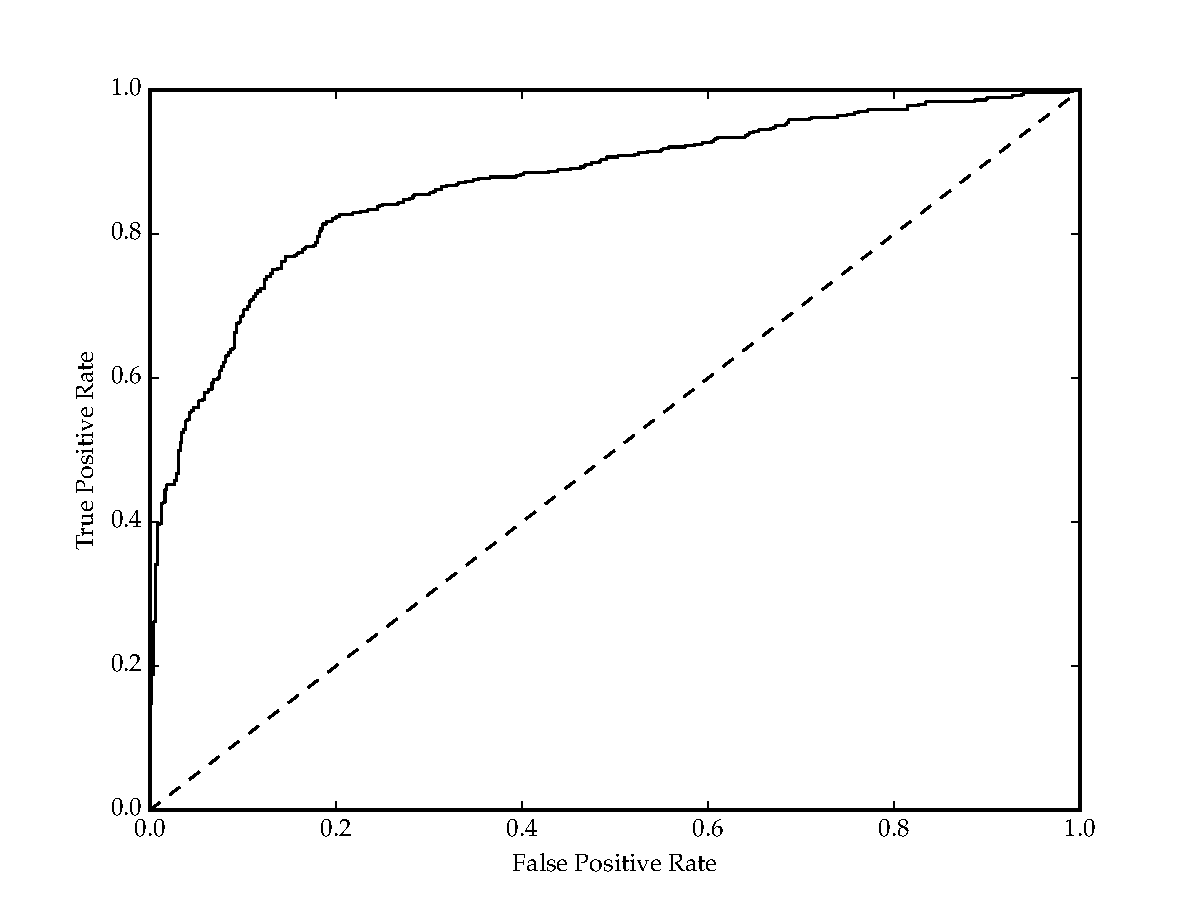
\includegraphics[width=.8\textwidth]{Figures/Chapter5/roc}
    \caption{An example of ROC curve. The dashed line is the ROC curve of a random classifier.}
    \label{fig:roc}
\end{figure}
To illustrate the behavior of the curve, it is useful to consider three extreme cases:
\begin{enumerate}
\item for a perfect classifier, which makes no errors, the curve goes from point $(0;0)$, to point $(1;0)$, to point $(1;1)$;
\item for a completely random classifier, which whatever the threshold always produces the same number of false positives and true positives, the curve created is the line segment bounded by the points $(0;0)$ and $\,(1;1)$;
\item no reasonable classifier is assumed to produce a ROC curve whose points are located under the $(0;0)$, $\,(1;1)$ segment.
\end{enumerate}
An AUROC value of 0.5 describes a completely random classifier (since it is equal to the area of the triangle described by the extreme case 2), while an AUROC of 1 describes a perfect classifier (since it is equal to the area of the square described by the extreme case 1). Good classifiers have an AUROC score generally equal or higher than 0.8. Besides being a metric independent of class proportions, the AUROC also offers a probabilistic interpretation of its value, since it is equals to the probability that the classifier will rank a randomly chosen positive example higher than a randomly chosen negative example. For an extensive survey of ROC curves, see for example \cite{?}.

\section{Results}
Here, we present the results obtained on the two experiments, \textbf{E1} and \textbf{E2}. Subsequently, we present an analysis of the performances obtained by the model on two use cases: one on synthetic data, and one on a real-world pathway.

\subsection{Results on the E1 Experiment}
Table \ref{tab:e1-results} shows the average accuracy on the 5 test folds obtained by each of the examined architectures on the \textbf{E1} experiment. Even though these results are obtained on a dataset approximately 15\% the size of the original one (consisting of 7036 induced subgraphs), we can already make some interesting observations about the task and the models:
\begin{itemize}
    \item the task can be learned, as evidenced by the gap between the baseline and all the examined models, which is approximately 13\% on average. This result verifies our initial assumption that it is indeed possible to predict robustness using only pathway structure;
    \item the comparison between the various \glspl{gcl} highlights the fact that there is no clear winner between the three tested architectures, which obtain very similar results when assessed on the same experimental conditions (\ie all models with/withour edge handling capabilities);
    \item as expected, adding edge handling to the \glspl{gcl} is beneficial to improve performances. On average, the models obtain a 1.8\% improvement in accuracy when edge handling is used.
\end{itemize}


\begin{table}[h!]
    \renewcommand\arraystretch{1.1}
    \caption{Results of the 5-fold CV evaluation of different \gls{dgn} architectures on the \textbf{E1} experiment, as explained in Section \ref{sec:pathway-experiments}. The suffix \quotes{-vanilla} indicates that the corresponding graph convolutional layer does not handle different edge contributions.}\label{tab:e1-results}
    \centering
    \begin{tabular}{lc}
        \toprule
            \Thead{Model}&  \Thead{Test Accuracy}\\
        \midrule
            Baseline & $0.7322\pm0.0000$\\
        \midrule
            GCN-vanilla & $0.8573\pm0.0087$ \\
            GIN-vanilla & $0.8567\pm0.0137$\\
            WLGCN-vanilla & $0.8624\pm0.0088$\\
        \midrule
            GCN & $0.8692\pm0.0140$\\
            GIN & $0.8684\pm0.0078$\\
            WLGCN & $0.8687\pm0.0117$\\
        \bottomrule
    \end{tabular}

\end{table}

In a second experiment, we assess whether depth (intendended as number of \gls{dgn} layers) is a good inductive for this task.To do so, we perform a \posthoc study the validation scores, to see how they relate to number of \gls{dgn} layers. Specifically, for each model, and for each number of layers from 1 to 8, we compute the average validation score obtained by all hyper-parameters configurations with an identical number of layers. Note that, although validation accuracy is in general an over-estimate of the true accuracy, the relative difference in performance as the number of layers change stays proportional independently of which specific data is used. In other words, we are not interested in the score by itself, but rather to the trend (increase or decrease) in performance in relation to the number of \gls{dgn} layers. Figure \ref{fig:e1-layering} clearly shows that, in all cases, increasing the number of layers improves accuracy, up to a certain depth (around 4-5 layers on average) where performances start to plateau. This provides evidence that depth is a good inductive bias for \glspl{dgn} on this task, up to some extent.

\begin{figure}[h!]
    \centering
    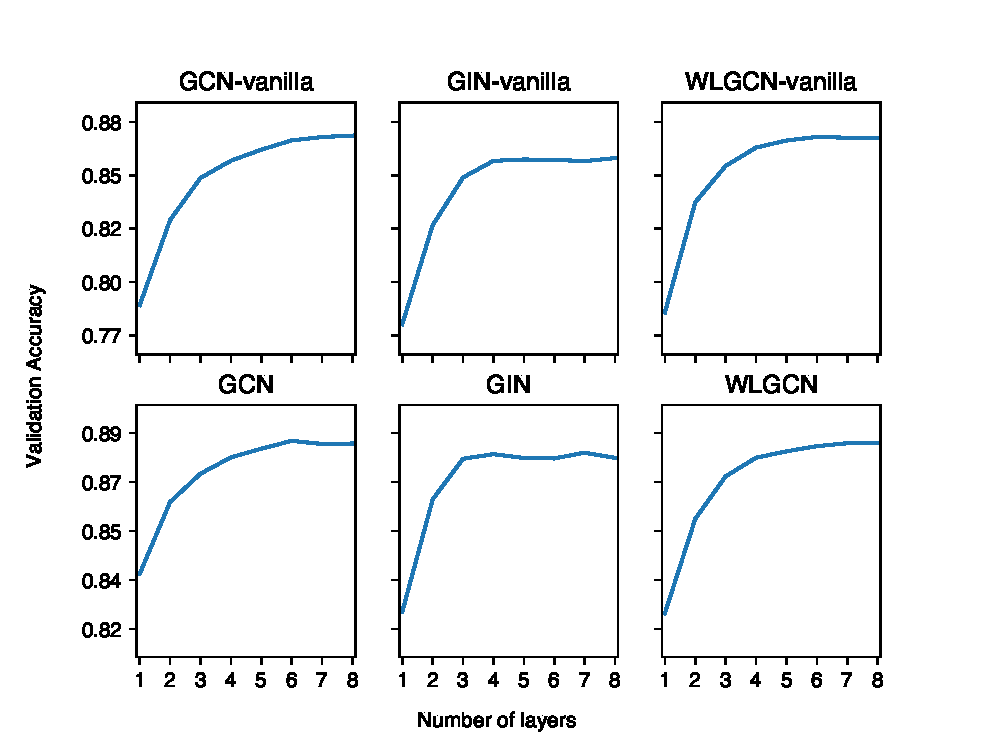
\includegraphics[width=.8\textwidth]{Figures/Chapter5/e1-layering}
    \caption{The effect of the number of \gls{dgn} layers to the performances of the models.}
    \label{fig:e1-layering}
\end{figure}

\subsection{Results on the E2 Experiments}\label{sec:e2-results}
For the second round of experiments, we fix the \gls{gcl} to the \gls{gcn} model with edge-handling capabilities, since it is the model that obtains the highest accuracy in \textbf{E1}.
The results of our experiments are reported in Table \ref{tab:e2-results}, where we average the computed metrics across the 5 test folds as usual.
\begin{table}[h!]
    \caption{Results of the 5-fold CV evaluation on various performance metrics. We report the global results (on the last row) as well as the results stratified by number of nodes per subgraph. For each stratification, we also report the related support (\ie the average number of graphs in the strata).}\label{tab:e2-results}
    \centering
    \footnotesize
    \renewcommand{\arraystretch}{1.2}
    \setlength{\tabcolsep}{0.7em}
    \begin{tabular}{lccccc}
      \toprule
      \Thead{Strata} & \Thead{Support} & \Thead{Accuracy} & \Thead{Sensitivity} & \Thead{Specificity} & \Thead{AUROC} \\
      \midrule
         1-10  & $243 (19)$ & $0.729 (0.020)$ & $0.851 (0.073)$ & $0.526 (0.113)$ & $0.820 (0.034)$\\
        11-20  & $711 (30)$ & $0.843 (0.006)$ & $0.919 (0.021)$ & $0.629 (0.050)$ & $0.892 (0.008)$\\
        21-30  & $526 (19)$ & $0.921 (0.008)$ & $0.969 (0.010)$ & $0.740 (0.052)$ & $0.954 (0.015)$\\
        31-40  & $967 (27)$ & $0.889 (0.012)$ & $0.937 (0.005)$ & $0.757 (0.040)$ & $0.950 (0.009)$\\
        41-50  & $1512 (21)$ & $0.928 (0.004)$ & $0.970 (0.008)$ & $0.635 (0.064)$ & $0.944 (0.011)$\\
        51-60  & $1679 (28)$ & $0.921 (0.004)$ & $0.971 (0.006)$ & $0.588 (0.038)$ & $0.950 (0.005)$\\
        61-70  & $1439 (23)$ & $0.947 (0.005)$ & $0.982 (0.006)$ & $0.644 (0.058)$ & $0.967 (0.005)$\\
        71-80  & $1159 (28)$ & $0.941 (0.006)$ & $0.980 (0.010)$ & $0.712 (0.087)$ & $0.972 (0.007)$\\
        81-90  & $372 (20)$ & $0.957 (0.008)$ & $0.998 (0.002)$ & $0.037 (0.075)$ & $0.925 (0.010)$\\
        91-100 & $378 (14)$ & $0.850 (0.017)$ & $0.964 (0.024)$ & $0.536 (0.061)$ & $0.888 (0.026)$\\
        \midrule
        \textbf{Overall} & $\mathbf{8985} (1)$ & $\mathbf{0.913} (0.003)$ & $\mathbf{0.965} (0.006)$ & $\mathbf{0.646} (0.042)$ & $\mathbf{0.948} (0.004)$\\
      \bottomrule
    \end{tabular}
\end{table}
In this case, we stratify the performances by number of nodes, in order to also analyze the model performances in relation to the size of the input subgraph. From the results, one can immediately see, by looking at the last row, how the model accurately predicts robustness better than all models tested in the \textbf{E1} phase by a large margin: this is probably caused by the largest size of the dataset, which usually results in major improvements with any \gls{ml} model, and in particular with \gls{dl} models. Specifically, we report an overall accuracy of $0.913 \pm 0.003$, as well as an AUROC of $0.948 \pm 0.004$. The model shows very high sensitivity ($0.965 \pm 0.006$) but a low specificity in comparison ($0.646 \pm 0.042$); this indicates that it is \quotes{harder} for the model to predict induced subgraphs that are not robust. This effect is a probable consequence of the class misproportion between negative and positive examples, which is around 86\% in favor of the positive class for this data sample. One result that is consistent across all measurements are the the very narrow standard deviations of the estimates, which indicate stable predictions regardless of the specific folds on which they are computed. To display this trend visually, we plot in Figure \ref{fig:e2-rolling-acc} the ROC curves obtained on the 5 test folds. Their similarity strongly indicates that the model performances are consistent across different test samples.
\begin{figure}
    \centering
    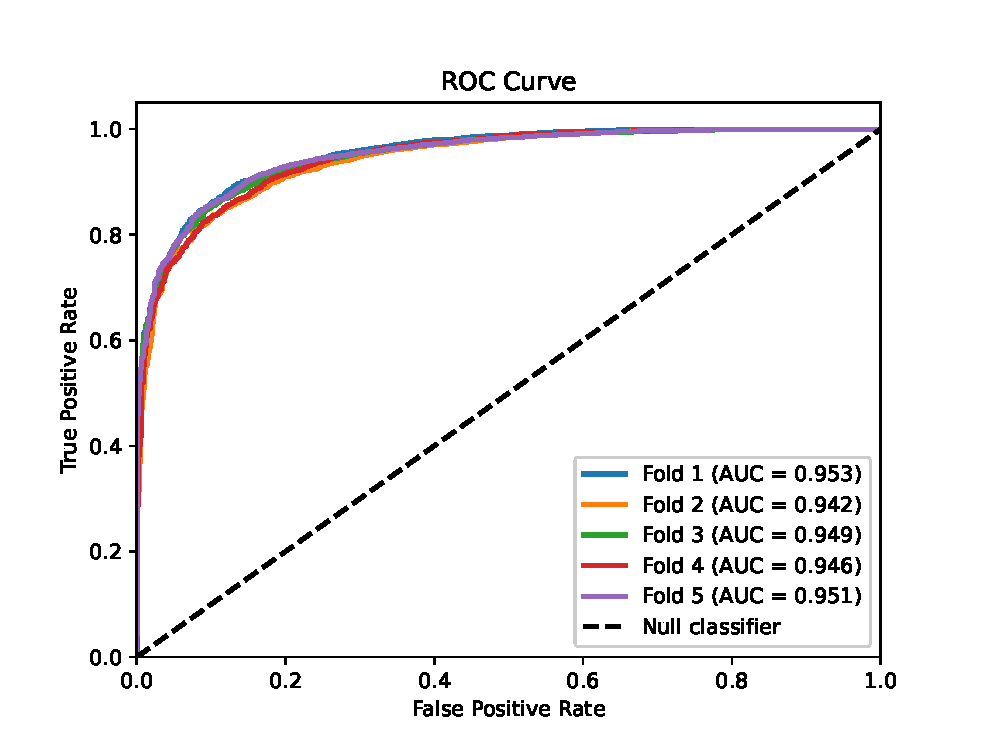
\includegraphics[width=.65\textwidth]{Figures/Chapter5/e2-roc-curve.eps}
    \caption{ROC curves for each of the five test folds. The black dashed line shows the performance of a baseline (\quotes{Null}) classifier that always predicts one class.}\label{fig:e2-roc-curve}
\end{figure}
The results of Table \ref{tab:e2-results} show a good performance of the model under the several stratifications tested. In particular, it performs better when dealing on subgraphs with 21-80 nodes, reaching an average in that strata AUROC of over 0.955. To better visualize this trend, we plot in Figure \ref{fig:e2-roc-curve} the rolling accuracy of the model, using a window size of 20, and averaging across the 5 test folds as usual. The plot clearly shows the improvement in accuracy as the number of nodes increases. Interestingly, when the size of the graph exceeds 80 nodes, the model performances start to decrease. This might be a consequence of the smaller sample sizes of subgraph with 81-100 nodes which occur in the dataset 3 times less on average than subgraphs with 21-80 nodes. The same trend can be noticed for smaller subgraphs, with up to 20 nodes. Finally, Figure \ref{fig:e2-conf-matrix} shows the confusion matrix of the predictions computed by the model, where the entries are the averages computed across the five test folds. In the plot, we can visualize the good performances of the model as regards the number of correctly predicted subgraphs (on the diagonal) with respect to the cases where the model makes wrong predictions. Looking at the anti-diagonal the confusion matrix, we can also see that the model has a higher rate of false positives than false negative. Again, this is expected behaviour due to class misproportion in the dataset.
\begin{figure}[h!]
    \begin{subfigure}[b]{0.48\linewidth}
    \centering
        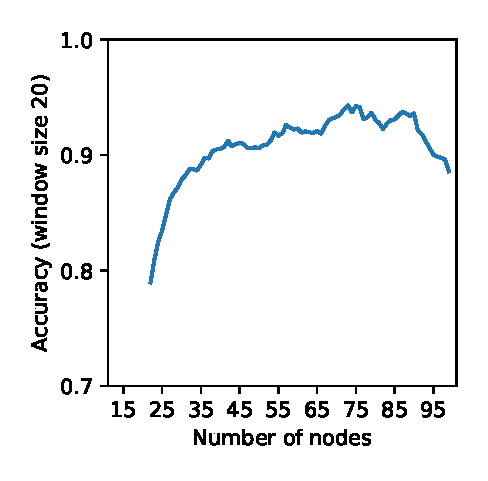
\includegraphics[height=130px]{Figures/Chapter5/e2-rolling-acc.eps}
        \subcaption{}\label{fig:e2-rolling-acc}
    \end{subfigure}
    %
    \begin{subfigure}[b]{0.48\linewidth}
        \centering
        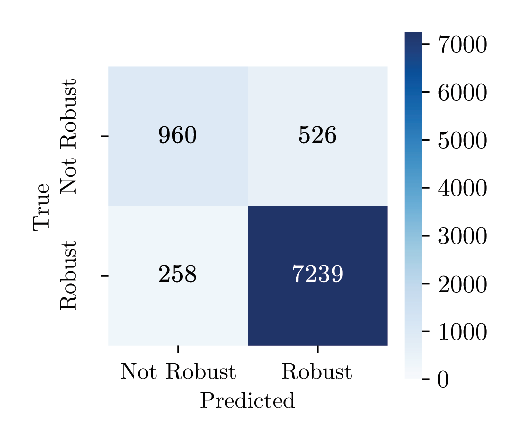
\includegraphics[height=130px]{Figures/Chapter5/e2-conf-matrix.eps}
        \subcaption{}\label{fig:e2-conf-matrix}
    \end{subfigure}
    \caption{({\scriptsize A}) Rolling mean accuracy (with a window of size 20), averaged over the 5 test folds, showing an increasing trend in performance as the number of graph nodes grows. ({\scriptsize B}) Confusion Matrix of the predictions computed by the model. Each entry of the matrix is the average of the corresponding entries in the five different confusion matrices of the test folds.}
\end{figure}

\subsection{Use Case on Synthetic Data}
The lower prediction accuracy in the case of small graphs (1-10 nodes) can be put into perspective, in light of the fact the fact we trained the model with subgraphs in which kinetic, stoichiometric and initial concentration parameters have been omitted (as explained in Section \ref{sec:ppn}). In general, the smaller the graph, the higher the influence on its dynamics these parameters exert. As an example, let us consider the synthetic example of biochemical pathway introduced in Figure \ref{fig:example-pathway} and the corresponding pathway graph of Figure \ref{fig:pathway-graph}. Let us now consider the following kinetic and initial concentration (marking) parameters:
\begin{gather*}
  k1 = 1.0 \quad
  k3 = 0.01 \quad
  k5 = 0.01 \quad
  k7 = 0.3  \quad
  k2 = 5.0  \quad
  k4 = 0.1  \quad
  k6 = 5.0 \\
  m_0(A) = 50\quad
  m_0(B) = 50\quad
  m_0(C) = 100\quad
  m_0(D) = 100\\
  m_0(E) = 0\quad
  m_0(F) = 0\quad
  m_0(G) = 100\quad
  m_0(H) = 0.
\end{gather*}
We used these parameters to simulate the ODEs of Figure \ref{subfig:example-odes}, calculating the corresponding robustness by varying the initial concentration of each molecule in the interval $[-20\%,+20\%]$. The robustness values obtained with the simulations are displayed in Table \ref{tab:uc1-odes}. Analogously, in Table \ref{tab:uc1-predictions} we list the average and standard deviations obtained by the 5 different models evaluated in Section \ref{sec:e2-results} (one trained on the respective CV fold), when tasked to predict the robustness probabilities of some input/output pairs of interest.
\begin{table}[h!]
    % \scriptsize
    \centering
    \caption{({\scriptsize A}) Robustness values computed by numerical simulation of the ODEs in Figure \ref{fig:example-pathway}. Input molecules with initial concentration equal to 0 are omitted. Output molecules with identical robustness values are merged. ({\scriptsize B}) Probabilities of robustness obtained from the model for some relevant input/output combinations.}
    \begin{subtable}[b]{.59\linewidth}
      \centering
        \begin{tabular}{cccccc}
            \toprule
            \multirow{2}{*}{\textbf{Input}} & \multicolumn{5}{c}{\textbf{Output}}\\
             & \SF{A} & \SF{B} & \SF{C/D} & \SF{E/F} & \SF{G/H}\\
            \midrule
              \SF{A} & 1.00 & 0.73 & 0.99 & 1.00  & 1.00  \\
              \SF{B} & 1.00 & 0.73 & 0.99 & 1.00  & 1.00  \\
              \SF{C} & 1.00 & 1.00  & 0.00  & 0.99 & 0.99 \\
              \SF{D} & 1.00 & 1.00  & 0.00  & 0.99 & 0.99 \\
              \SF{G} & 1.00 & 1.00  & 1.00  & 1.00  & 0.50  \\
            \bottomrule
        \end{tabular}
        \caption{}\label{tab:uc1-odes}
    \end{subtable}%
    \begin{subtable}[b]{.39\linewidth}
        \centering
        \begin{tabular}{cc}
            \toprule
            \Thead{In/Out} & \Thead{Probability}\\
            \midrule
                $\SF{B}/\SF{A}$ & $0.3798 \pm 0.12$\\
                $\SF{A}/\SF{F}$ & $0.7254 \pm 0.18$\\
                $\SF{A}/\SF{H}$ & $0.8835 \pm 0.05$\\
                $\SF{C}/\SF{F}$ & $0.0793 \pm 0.11$\\
                $\SF{G}/\SF{H}$ & $0.2351 \pm 0.01$\\
            \bottomrule
        \end{tabular}
        \caption{}\label{tab:uc1-predictions}
    \end{subtable}
\end{table}
We remark that values in these two tables are not directly comparable: those in Table \ref{tab:uc1-odes} are exact robustness values, while those in Table \ref{tab:uc1-predictions} are probabilities of the robustness values to be greater than 0.5. In this specific case, the prediction turns out to be accurate in the case of input/output pairs corresponding to big induced subgraphs. This happens in the cases of the input/output pairs $A/F$ and $A/H$, whose induced subgraphs are among the largest ones. In contrast, the prediction is incorrect for $C/F$: in this case, the models predicts a small robustness probability, while the simulations give 0.99. We observe that the robustness value of this input/output combination is sensitive to the perturbation of parameters that have been discarded when constructing the dataset. In particular, if the initial (omitted) concentration of $C$ was $80$ instead of $100$, the robustness value of the pair $C/F$ would become $0.5$ rather than $0.99$. Another case when the model prediction is wrong is that of the pair The prediction turns out to be wrong also in the case of input $B/A$. In this case, the probability given by the network is under $0.50$, which contrasts to a value of $1$ obtained by the ODEs simulation. Even in this case, we notice that the parameters that have been omitted in the dataset might have a strong influence on the robustness, such as kinetic formulas and the multiplicity of the edge directed to node $B$. Finally, in the case of the pair $G/H$, the prediction gives a small probability of robustness and indeed the actual measured value is borderline ($0.50$). More in general, we observe that smaller subgraphs are less frequent than medium-sized subgraphs in the dataset. Thus, it is possible that the model has learned to be more accurate on the latter subgraphs (to maximize the accuracy), at the expense of making more errors when predicting the former.
\part{Deep Generative Learning on Graphs with Applications to Computational Chemistry}

%----------------------------------------------------------------------------------------
%	THESIS CONTENT - APPENDICES
%----------------------------------------------------------------------------------------

\appendix % Cue to tell LaTeX that the following "chapters" are Appendices

% Include the appendices of the thesis as separate files from the Appendices folder
% Uncomment the lines as you write the Appendices

% Appendix A

\chapter{Frequently Asked Questions} % Main appendix title

\label{AppendixA} % For referencing this appendix elsewhere, use \ref{AppendixA}

\section{How do I change the colors of links?}

The color of links can be changed to your liking using:

{\small\verb!\hypersetup{urlcolor=red}!}, or

{\small\verb!\hypersetup{citecolor=green}!}, or

{\small\verb!\hypersetup{allcolor=blue}!}.

\noindent If you want to completely hide the links, you can use:

{\small\verb!\hypersetup{allcolors=.}!}, or even better: 

{\small\verb!\hypersetup{hidelinks}!}.

\noindent If you want to have obvious links in the PDF but not the printed text, use:

{\small\verb!\hypersetup{colorlinks=false}!}.

%\chapter{List of Publications}\label{AppendixB}

\begin{itemize}
\item F. Errica, M. Podda, D. Bacciu, A. Micheli. "A Fair Comparison of Graph Neural Networks for Graph Classification".
\textit{8th International Conference on Learning Representations (ICLR)}. (2020)
\item M. Podda, D. Bacciu, A. Micheli. "A Deep Generative Model for Fragment-Based Molecule Generation". \textit{Proceedings of the Twenty Third International Conference on Artificial Intelligence and Statistics (AISTATS)}. Vol. 108, pages 2240-2250. (2020)
\item D. Bacciu, F. Errica, A. Micheli, M. Podda. "A Gentle Introduction to Deep Learning for Graphs". \textit{Neural Networks}. Volume 129, Pages 203-221. ISSN 0893-6080, doi:10.1016/j.neunet.2020.06.006. (2020)
\item P. Bove, P. Milazzo, A. Micheli, M. Podda.
"Prediction of dynamical properties of biochemical pathways with Graph Neural Networks". \textit{Proceedings of the 13th International Joint Conference on Biomedical Engineering Systems and Technologies - Volume 3: BIOINFORMATICS}. ISBN 978-989-758-398-8, pages 32-43. doi:10.5220/0008964700320043 (2020)
\item M. Podda, D. Bacciu, A. Micheli, P. Milazzo. "Biochemical Pathway Robustness Prediction with Graph Neural Networks". \textit{To appear in: ESANN 2020 Proceedings} (2020)
\item D. Bacciu, A. Micheli, M. Podda. "Edge-based sequential graph generation with recurrent neural networks". \textit{Neurocomputing},
Volume 416, pages 177-189, ISSN 0925-2312. doi:10.1016/j.neucom.2019.11.112. (2020)
\item D. Bacciu, A. Micheli, M. Podda. "Graph generation by sequential edge prediction". \textit{ESANN 2019 Proceedings}, pages 95-100, ISBN 978-287-587-065-0. (2019)
\item M. Podda, D. Bacciu, A. Micheli, R. Bellù, G. Placidi, L. Gagliardi. "A machine learning approach to estimating preterm infants survival: development of the Preterm Infants Survival Assessment (PISA) predictor". \textit{Sci Rep} 8, 13743. doi:10.1038/s41598-018-31920-6 (2018)
\end{itemize}
%\chapter{Contributed Code}\label{AppendixC}

\begin{itemize}
    \item Code for the article: M. Podda, D. Bacciu, A. Micheli, R. Bellù, G. Placidi, L. Gagliardi. "A machine learning approach to estimating preterm infants survival: development of the Preterm Infants Survival Assessment (PISA) predictor". \textit{Sci Rep} 8, 13743. doi:10.1038/s41598-018-31920-6 (2018)\\
    URL: \url{https://github.com/marcopodda/inn}
    \item Code for the article: D. Bacciu, A. Micheli, M. Podda. "Edge-based sequential graph generation with recurrent neural networks". \textit{Neurocomputing},
    Volume 416, pages 177-189, ISSN 0925-2312. doi:10.1016/j.neucom.2019.11.112. (2020)\\
    URL: \url{https://github.com/marcopodda/grapher}
    \item Code for the conference paper: M. Podda, D. Bacciu, A. Micheli. "A Deep Generative Model for Fragment-Based Molecule Generation". \textit{Proceedings of the Twenty Third International Conference on Artificial Intelligence and Statistics (AISTATS)}. Vol. 108, pages 2240-2250. (2020)\\
    URL: \url{https://github.com/marcopodda/fragment-based-dgm}
    \item Code for the conference paper: F. Errica, M. Podda, D. Bacciu, A. Micheli. "A Fair Comparison of Graph Neural Networks for Graph Classification".
    \textit{8th International Conference on Learning Representations (ICLR)}. (2020)\\
    URL: \url{https://github.com/diningphil/gnn-comparison}
\end{itemize}

%----------------------------------------------------------------------------------------
%	BIBLIOGRAPHY
%----------------------------------------------------------------------------------------

\printbibliography[heading=bibintoc]

%----------------------------------------------------------------------------------------

\end{document}  
